\documentclass{dissertation}
%\documentclass[print]{dissertation}
%\documentclass[print,draft]{dissertation}
\usepackage{fontspec}
\usepackage{fontawesome}

\hyphenation{TestRoots WatchDog proj-ect proj-ects Ec-lipse two-fold clie-nts Mo-cki-to wide-spread pro-vers Bent-kamp}
\newcommand{\sparkline}[1]{$\vcenter{\hbox{\includegraphics[scale=0.04]{#1}}}$}


\makeglossaries

\newcommand*{\origrightarrow}{}
\let\oldarrow\textrightarrow
\renewcommand*{\textrightarrow}{\fontfamily{cmr}\selectfont\origrightarrow}
\loadglsentries[main]{glossary}

\usepackage{enumitem}



\usepackage{xspace}

\newcommand{\eq}{\approx}
\newcommand{\noteq}{\napprox}

\newcommand\cst[1]{\mathsf{#1}}
\newcommand\imp{\ensuremath{\rightarrow}}
\newcommand\lequiv{\ensuremath{\leftrightarrow}}

\newcommand{\lland}{\mathrel\land}
\newcommand{\llor}{\mathrel\lor}
\newcommand{\newehoh}{\ensuremath{\lambda}E}

\newcommand{\tuple}[2]{\overline{#1}_{#2}}
\newcommand{\tuplen}[1]{\overline{#1}_{n}}

\newcommand{\lam}[2]{\ensuremath{\lambda #1.\> #2}}
\newcommand{\lamx}[1]{\lam{x}{#1}}

\newcommand{\ifalse}{\pmb\bot}
\newcommand{\itrue}{\pmb\top}
\newcommand{\inot}{\pmb{\neg\,}}
\newcommand{\iand}{\pmb\land}
\newcommand{\ior}{\pmb\lor}
\newcommand{\iimplies}{\pmb\rightarrow}
\newcommand{\iequiv}{\pmb\leftrightarrow}
\newcommand{\iforall}{\pmb\forall}
\newcommand{\iexists}{\pmb\exists}
\newcommand{\ieq}{\pmb\approx}
\newcommand{\ineq}{\pmb{\not\approx}}
\newcommand{\equi}{\leftrightarrow^*_{\alpha\beta\eta}}


\newcommand{\neglit}[1]{\ensuremath{#1 \noteq \itrue}}
\newcommand{\poslit}[1]{\ensuremath{#1 \eq \itrue}}

\newcommand{\substterm}[2]{\ensuremath{#1(#2)}}
\newcommand{\sigmaterm}[1]{\ensuremath{\substterm{\sigma}{#1}}}

\newcommand{\substcl}[2]{\ensuremath{#2#1}}
\newcommand{\sigmacl}[1]{\ensuremath{\substcl{\sigma}{#1}}}

\newcommand\unif{\mathrel{\smash{\stackrel{\lower.1ex\hbox{\ensuremath{\scriptscriptstyle ?}}}{=}}}}


\newcommand\infname[1]{\textsc{#1}}
% Inference rule
\newcommand{\namedinference}[3]{\prftree[r]{\relax{\infname{#1}}}{\strut#2}{\strut#3}}
\newcommand{\inference}[2]{\namedinference{}{\strut#1}{\strut#2}}

% Simplification rule
\newcommand{\namedsimp}[3]{\prftree[d][r]{\relax{\infname{#1}}}{\strut#2}{\strut#3}}
\newcommand{\simp}[2]{\namedinference{}{\strut#1}{\strut#2}}
\newcommand{\ourmodel}{\ensuremath{\mathscr{J}}}
\newcommand{\NumberOK}[1]{#1}

\newcommand{\lfhol}[0]{$\lambda$fHOL}
\newcommand{\appvar}[0]{\ensuremath{\mathsf{@}}}


\begin{document}

%% Specify the title and author of the thesis. This information will be used on
%% the title page (in title/title.tex) and in the metadata of the final PDF.
\title{Implementation of Higher-Order Superposition}
\author{Petar}{Vukmirović}

%% Use Roman numerals for the page numbers of the title pages and table of
%% contents.
\frontmatter

% For VSCode
% !TEX root = ../dissertation.tex
\begin{titlepage}

% \begin{center}

% %% Extra whitespace at the top.
% \vspace*{2\bigskipamount}

% %% Print the title.
% {\makeatletter
% \titlestyle\bfseries\LARGE\@title
% \makeatother}

% %% Print the optional subtitle.
% {\makeatletter
% \ifx\@subtitle\undefined\else
%     \bigskip
%     \titlefont\titleshape\Large\@subtitle
% \fi
% \makeatother}

% \end{center}

\cleardoublepage
\thispagestyle{empty}

\begin{center}

%% The following lines repeat the previous page exactly.

\vspace*{2\bigskipamount}

%% Print the title.
{\makeatletter
\titlestyle\bfseries\LARGE\@title
\makeatother}

%% Print the optional subtitle.
{\makeatletter
\ifx\@subtitle\undefined\else
    \bigskip
    \titlefont\titleshape\Large\@subtitle
\fi
\makeatother}

%% Uncomment the following lines to insert a vertically centered picture into
%% the title page.
%\vfill
%\includegraphics{title}
\vfill

%% Apart from the names and dates, the following text is dictated by the
%% promotieregelement.

{\Large\titlefont\bfseries Proefschrift}

\bigskip
\bigskip

ter verkrijging van de graad van doctor

aan Vrije Universiteit Amsterdam,

op gezag van de Rector Magnificus prof.dr.~J.J.G.~Geurts,

voorzitter van het College voor Promoties,

in het openbaar te verdedigen

op [onbekend]

\bigskip
\bigskip

door

\bigskip
\bigskip

%% Print the full name of the author.
\makeatletter
{\Large\titlefont\bfseries\@firstname\ \titleshape{\MakeUppercase{\@lastname}}}
\makeatother

\bigskip
\bigskip

Master of Science in Computer Science, \\
Vrije Universiteit Amsterdam, Nederland,

geboren te Belgrado, Servi\"e.

%% Extra whitespace at the bottom.
\vspace*{2\bigskipamount}

\end{center}

\clearpage
\thispagestyle{empty}

%% The following line is dictated by the promotieregelement.
\noindent Dit proefschrift is goedgekeurd door de

%% List the promotors (supervisors).
\medskip\noindent
\begin{tabular}{ll}
    promotor: & prof.$\,$dr. W. J. Fokkink \\
    copromotoren: & dr. J. C. Blanchette \\
                  & prof.$\,$dr. S. Schulz
\end{tabular}

\bigskip
\noindent Samenstelling promotiecommissie:

%% List the committee members, starting with the Rector Magnificus and the
%% promotor(s) and ending with the reserve members.
\medskip\noindent
\begin{tabular}{p{4.5cm}l}

prof.$\,$dr. M. Hoogendoorn & Vrije Universiteit Amsterdam \\
dr. K. Korovin & The University of Manchester \\
dr. R. Piskac & Yale University \\
dr. A. Steen & University of Greifswald \\
dr. M. Suda & Czech Technical University in Prague \\
prof.$\,$dr. G. Sutcliffe & University of Miami \\

\end{tabular}

%% Include the following disclaimer for committee members who have contributed
%% to this dissertation. Its formulation is again dictated by the
%% promotieregelement.
%\medskip
%\noindent  %Prof.\ Dr.\ D.\ Spinellis has contributed to the creation of this thesis.

\medskip
\medskip
% TODO Include http://www.win.tue.nl/ipa/?page_id=309
\noindent The work in the thesis has been carried out under the auspices of the research school IPA
(Institute for Programming research and Algorithmics).

\medskip
%% Here you can include the logos of any institute that contributed financially
%% to this dissertation.
\vfill
\begin{center}
    
\includegraphics[height=0.5in]{title/logos/vulogo}
    \hspace{2em}
    %\includegraphics[height=0.5in]{title/logos/casimir} \\
    
\includegraphics[height=0.5in]{title/logos/erclogo}
    \\ \vspace{0.5cm}
    \includegraphics[height=0.5in]{title/logos/ipa}
\end{center}
\vfill

\noindent
\begin{tabular}{@{}p{0.2\textwidth}@{}p{0.8\textwidth}}
  \textit{Keywords:} &  \\[\medskipamount]
      \textit{Printed by:} &  \\[\medskipamount]
      \textit{Cover:} &  Marina Abramović, Rhythm 10 (The Biography), Cibachrome Print,
                         1997, © Marina Abramović,
                         Courtesy of the Marina Abramović Archives \\[\medskipamount]
      \textit{Style:} & TU Delft House Style, with modifications by Moritz Beller \\& \url{https://github.com/Inventitech/phd-thesis-template} \\[\medskipamount]
\end{tabular}

\medskip
\medskip
\noindent The author set this thesis in \LaTeX\xspace using the Libertinus Serif, Inter and Inconsolata fonts.

\vspace{\bigskipamount}

% Copyrighting this is stupid, questionable, and probably illegal, because large parts of the
% thesis have already been published with the copyright resigning with the publisher.
%\noindent Copyright \textcopyright\ 2015 by A.~Einstein

%% Uncomment the following lines if this dissertation is part of the Casimir PhD
%% Series, or a similar research school.
%\medskip
%\noindent Casimir PhD Series, Delft-Leiden 2015-01

%\medskip
\noindent ISBN \ldots

\medskip
% \noindent An electronic version of this dissertation is available at \\
% \url{http://repository.tudelft.nl/}.

\end{titlepage}



% %% The (optional) dedication can be used to thank someone or display a
% %% significant quotation.
% \dedication{\epigraph{I [...] like to give the maximum in everything I do. The maximum I have. The
%     maximum I can give. I am not perfect. But if I do something, I do it [as best I can].
%     %And many people are not made like this. There are only few. But I like these few.
%   }{Reinhold Messner}}

\tableofcontents

\chapter*{Summary}
\addcontentsline{toc}{chapter}{Summary}
\setheader{Summary}

\looseness=-1
In the last decades, proof assistants were immeasurably useful in formally
proving validity of hard mathematical theories and correctness of
safety-critical software. These tools provide a formal language that allows one
to describe a problem and prove statements about it which are later
automatically checked. To make the checking phase efficient and trustworthy,
proof steps need to be of high granularity. As a consequence, seemingly
simple statements must be proven in minute detail, making the use of proof
assistants very tedious.

In an attempt to automate significant parts of this proving process, assistants
can invoke automatic theorem provers to finish the proof. However, most
assistants are based on higher-order logic, while most automatic theorem provers
are based on first-order logic. This means that the two systems must communicate
through translations, which obfuscate the problem and likely make it more
difficult than it originally was.

In this thesis, we try to bridge this translation gap. We start from E, one of the best
first-order proof assistants backends, based on the superposition calculus, and
gradually extend it to higher-order logic. As this approach is large in scope,
we split it in three parts.

The first part extends E to support a fragment of higher-order logic devoid of
$\lambda$-abstra\-ction, yielding a prover called Ehoh. Even though this extension
is arguably conservative, Ehoh shows stronger performance on proof assistant
benchmarks than E.

The second part concerns adding support for $\lambda$-abstraction. The most
important challenge we faced during this extension is that of higher-order
unification. At the time we started, state-of-the-art procedure
for full higher-order unification was developed in 1970s. We designed a new
procedure inspired by this one that enumerates less redundant unifiers, has many
modern optimizations built-in, and can easily be customized to trade its
completeness for performance. It is implemented in a
prototype prover Zipperposition, a less efficient, but more easily extendible
prover compared to E. Our evaluation shows that our
procedure substantially improves on state-of-the-art.

The last part concerns adding support for
first-class Boolean terms. For this part we took inspiration from traditional
automatic higher-order provers, based on tableaux. We fitted those techniques in
superposition context and implemented them in Zipperposition. They
made Zipperposition the best prover in the higher-order division of the annual CASC
theorem prover competition for two consecutive years.

After testing out our ideas in Zipperposition, we decided to go back to Ehoh and
extend it to full higher-order logic, obtaining a prover called \ehohii{}. We
choose the most successful approaches implemented in Zipperposition that can
easily be ported to \ehohii{}. The results were once again positive: Our
evaluation shows that \ehohii{} is the best prover on proof assistant
benchmarks, and second only to Zipperposition on a standard benchmark set.

We took our idea of porting techniques from weaker to stronger logics one step
back: We explored SAT simplification techniques that can be implemented in the
superposition context. We discovered that while some of them can be used during proving,
most of them work best as preprocessors.


\chapter*{Samenvatting}
\addcontentsline{toc}{chapter}{Samenvatting}
\setheader{Samenvatting}

{\selectlanguage{dutch}


}




\chapter*{Preface}
\addcontentsline{toc}{chapter}{Preface}
\setheader{Preface}

When I downloaded the \LaTeX{} template to write this thesis, the following
sentence was present as a placeholder:
\begin{quote}
    Without a doubt, the acknowledgments are the most widely and most eagerly
    read part of any thesis.
\end{quote}
\noindent
I do not know if that is true in general, but I have to admit I am guilty of
spending quite some time reading acknowledgments. I find that the reason why we
spend so much time reading acknowledgments is that we want to peek behind the
rigorous, formal shape that a PhD thesis is required to take. We also want to
see what PhD candidates have to say about their personal experiences of
finishing a PhD.

After reading many preface or acknowledgments chapters I realized that there
is a discrepancy between what research shows candidate's experience of finishing
a PhD is and what is actually written in these parts of theses. An
article by Levecque et al. \cite{labhg-17-phdstudents} states that one in two
PhD students experiences psychological distress, while one in three is at risk
of a common psychiatric disorder. In the light of this fact, I want to write
this chapter not only to the people whose help and work indebted me, but also to
(future) PhD students that, after looking up a detail in this thesis,
voyeuristically read this chapter (like I did many times for other theses).

In my first year of PhD, I was overwhelmed with fear and doubts. Did I make the
right choice by starting a PhD? Am I performing up to expectations? How many
papers should I publish? Should I read more papers? Did I \emph{actually} learn
anything? I could go on an on like this.

The fact that I was surrounded by very successful postdocs and PhD students on
later years of their studies made me feel like I was the only one having this
problem. To the students reading this chapter, I would very much like to assure
you that you are not. 

What helped me go out of the self-doubting loop was actually taking action. From
the simplest ones, like saying ``I don't understand'' out loud instead of
silently nodding when I have a trouble following scientific discussion, to the
ones with more impact on my career like actively looking for projects I could
join while I did not have much work on my plate. As the years went on I felt
that I could more openly talk about my insecurities and I found out that many
people in my situation have them as well.

What made my PhD journey more enjoyable are undoubtedly the people I worked
with. I want to thank the whole Theoretical Computer Science group at the VU
which was there with me from the early days of my master studies. They helped me
organize my master programme so that I follow more theory courses which most
likely lead  me to start an academic career. I also want to thank other postdocs
and PhDs that studied during my PhD or are still studying. Most notably, I would
like to thank Alexander Bentkamp, one of the most gifted mathematicians I know.
I coauthored many of my papers with him, each of which was a pleasure to work
on. I would also like to thank all of my collaborators and people that suggested
improvements to the articles I wrote.

I want to thank my daily supervisor, Jasmin Blanchette. He always says that the
main product of a PhD is not a thesis but a person you come out as after four
years. With his guidance, I learned to approach things more rigorously, slower,
and with more attention. He also helped me tremendously  with my writing and
presentation skills. Even though he tried very hard, he did not teach me to use
articles (i.e., English articles ``the'', ``a'', or ``an'') though, and
capitulated by adding them to many of the articles I wrote.

My other two supervisors also helped me greatly. Wan Fokkink read the thesis
very carefully and provided very valuable comments. For the last four years he
made my PhD a smooth sail by solving all the administrative issues on time and
provided a very nice work environment. Stephan Schulz is a real programming and
logic wizard. His deep understanding of all things superposition and low-level
Linux programming helped me not only with my PhD, but I also learned a lot of
new skills that are undoubtedly useful for my future career.

Predrag Jani\v{c}i\'{c}, my professor from University of Belgrade who 
inspired me to deepen my knowledge in various areas of computer science, suggested
many improvements to the text of this thesis. I thank him as well.

Lastly, I would like to thank Martijn. He was besides me for the last four years
and helped me overcome many of the doubts and issues I mentioned. He also always
patiently waits until my medication or second glass of Grüner Veltliner kick in
(not at the same time). I also want to thank Jelisaveta and Tara, which
sometimes had to deal with me when medication or wine did not kick in. All my other friends,
in Serbia or the Netherlands, thank you for your support.

 

\begin{flushright}
{\makeatletter\itshape
    Petar \\
    Amsterdam, April 2022
\makeatother}
\end{flushright}




%% Use Arabic numerals for the page numbers of the chapters.
\mainmatter

%% Turn on thumb indices.
\thumbtrue

\chapter{Introduction}
\setheader{Introduction}
\label{ch:intro}

Half sleeping, half playing Fruit Ninja on my smartphone at one of the
philosophy lectures in my high school I heard my professor exclaim with
excitement: “Mathematical truth is the highest form of truth!”.
Unbothered and uninterested, I continued playing Fruit Ninja.

Many years later I started studying various formal methods in computer science.
There I learned the value of formal, mathematical language and finally
understood him. Not only does using a rigorous mathematical language avoid the
ambiguity of the natural one, it allows us to use the formal rules of reasoning
to make conclusions from initial arguments in a trustworthy manner. 

Though the interest for rigorous and formal reasoning dates back to Aristotle,
it intensified at the end of 19th and the beginning of 20th century
\cite{jf-01-modern-logic}. Researchers in that time were mostly interested in
finding a formal language that is expressive enough to describe complex
mathematical theories, yet intuitive and understandable enough to allow
reasonably simple formal reasoning systems. First-order logic seemed to satisfy
both requirements.  This formalism does not only allow one to model simple
logical relations such as ``if it rains, the road is muddy'' (or formally
$\cst{rains} \imp \cst{muddy}$), but also to quantify over objects as in ``all
people are mortal'' ($\forall x.\, \cst{human}(x) \imp \cst{mortal}(x)$).

\paragraph{Automatic Theorem Proving}The initial study of first-order logic and the rules to reason about statements in
it was very prolific. In 1930 G\"odel \cite{kg-30-completeness-theorem} showed
that there is a system of inference rules (calculus) such that for any valid
statement a proof of validity can be constructed in this system. Around the same
time, the first computers were leaving the imagination of the engineers and
began automating many complicated processes.  Naturally, the question as to
whether a computer can decide if a first-order statement is valid (i.e., a
theorem) arose. Church \cite{ac-36-fol-undecidable} and Turing
\cite{tm-37-undecidable} answered this question negatively in 1936.

Despite this negative result, the prospect of automatically proving theorems of
first-order logic remained too enticing. In 1960, Davis and Putnam
\cite{dp-1960-dpll} described a procedure for checking validity of a
first-order formula. As first-order logic is undecidable, this procedure
terminated only on valid formulas. Even though it was efficient enough to prove
only simple formulas, it was an impressive achievement for the time.

A bigger breakthrough happened in 1965 when Robinson introduced a calculus that
would shape the future of automatic reasoning --- the resolution calculus
\cite{ar-65-resolution}. Consisting of a single inference rule it was simple and
elegant. It was also \emph{complete}: each theorem could be proven using this
system. Furthermore, it was less explosive than Davis and Putnam's algorithm
since it introduced unification as an inference filter.

Since its introduction, resolution was improved in many ways. Strategies and
heuristics~\cite{lw-65-sos} to curb the explosion of the search space were
introduced, as well as complete, but less explosive variants of the calculus
\cite{cc-73-resolution-book}. Despite this progress, reasoning about equality of
objects was still hard for these methods. This changed with introduction of
superposition~\cite{bg-94-superposition} in the early 1990s.

Superposition is a complete calculus for first-order logic loosely based on
resolution, featuring support for equality on the calculus level. This support
is further optimized by use of term orders and selection functions to prune the
search space. Thanks to efficient implementation, this calculus was used to
prove long-standing open problem known as ``Robbins conjecture''
\cite{mccune-97-robbins}. Provers based on this calculus have been
winning the first-order division of CASC theorem proving competition since its
inception in the 1990s \cite{ss-96-casc}.

Even though the successes of proving Robbins conjecture showed that it is
possible, automatically proving hard mathematical problems is still out of reach
for theorem provers. However, there are other ways in which humans and computers can work together to construct formal
proofs.

\paragraph{Proof Assistants and Hammers} Proof assistants (or interactive
theorem provers) are programs which allow users to describe a theory formally
and to write proofs of the statements about this theory using inference 
rules of the proof assistant. These programs can then check if the given proof
is correct. As their core is usually small and well-tested, proofs that pass the
checking phase are considered trustworthy.

Proof assistants showed indispensible in proving very complex mathematical theorems in a
trustworthy manner. For example, four-color theorem \cite{gg-2008-four-color}
and Kepler conjecture \cite{th-2015-kepler} were proven inside proof assistants,
ending the need to trust hundreds of pages of hard mathematical proofs. Proof
assistants are also used to show correctness of complex software such as
compilers \cite{xl-09-compcert} or operating systems kernels \cite{gk-09-sel4}.
This verified software can be used in safety-critical scenarios such as nuclear
plants or autonomous vehicles.

The proofs need to be spelled out in minute detail to be accepted by a proof assistant.
Even though many proof assistants offer some sort of automation, seemingly simple
statements cannot be automatically proved. This is one of the reasons why large
verification projects can take years to finish.

Integrating proof automation right into the proof assistant is not an easy task.
Most proof assistants are based on variants of higher-order logic, which is more
expressive than first-order logic, but harder to automate as in general it does not even allow complete
proof calculi. To provide some level of automation, proof assistant developers
use the efficient first-order provers as follows. First, the proof goal is
translated from higher-order to first-order logic. Then the first-order prover
is run on the translated problem. If the first-order prover finds the proof, the
proof is reconstructed in the proof assistant. This approach is implemented in
modern assistants such as Coq \cite{bc-04-coq}, HOL Light \cite{jh-09-hol-light}
and Isabelle \cite{lc-88-isabelle} using \emph{hammers} CoqHammer
\cite{ck-18-coqhammer}, HOL(y)Hammer \cite{ku-15-holyhammer} and Sledgehammer
\cite{bn-10-sh}, respectively. 

The approach proved useful: around 76\% of the simple proof goals can be
discharged automatically using Sledgehammer \cite{bgkku-16-larning-fact-selector}. However, there is
clearly some untapped potential in the approach as it communicates with
automatic theorem provers through a translation. To bridge this translation gap,
attempts were made to use higher-order automatic theorem provers instead of
first-order ones \cite{ns-13-leo2sh}. This proved unfruitful as state-of-the-art
higher-order theorem provers of the time were primarily designed for small and
tricky problems. On the other hand, problems coming from hammers consist of
mostly first-order formulas, are rather large, and mostly require simple
higher-order proof steps. Thus, from a standpoint of proof assistant ideal
automatic theorem prover fulfills the following wishlist:
\begin{enumerate}
  \item\label{it:fo} Performs as best first-order provers on first-order problems
  \item\label{it:size} Scales well with the size of the problem
  \item\label{it:ho} Supports higher-order logic and scales with the amount of higher-order axioms
\end{enumerate}
This brings us to the topic of this thesis: \emph{How to develop a prover fulfilling this wishlist?}

\paragraph{Our Approach} To improve the automatic reasoning for higher-order
logic we decided not to start from a blank slate and build a new theorem prover.
Rather, we start from a position of strength --- from state-of-the-art
first-order superposition theorem prover E \cite{scv-19-e23} --- and extend this
prover to higher-order logic. In this way, the points \ref{it:fo} and
\ref{it:size} from the above wishlist are already fulfilled, as E is very
efficient and deals well with large problems.

We do not extend E to higher-order logic in one atomic step. Instead, we extend
it by adding support for features of higher-order logic one by one,
which gradually increase its reasoning capabilities. With this gradual
approach we make sure that after every extension, E's
efficiency on first-order problems did not decrease. Thus, while trying
to fulfill the point \ref{it:ho} from the wishlist we make sure that points
\ref{it:fo} and \ref{it:size} are not affected.

We have split the road to full higher-order logic in three stages. A
distinguished feature of higher-order logic is that it not only supports
quantification over objects, but also over functions that manipulate these
objects. Thus, higher-order logic allows us to make a statement ``all functions
with arguments $0$ and $1$ result in $2$" ($\forall x. \,  x (\cst{0}, \cst{1}) \eq
\cst{2}$). Replacing $x$ with addition function ($\cst{+}$) is enough to
disprove this statement. The first stage is to extend E to support
quantification over functions that are already present in the theory.

Higher-order logic also supports expressing functions that are not explicitly
present in the theory. Suppose we want to prove that there is a
function that returns 4 when given 2 and 5 when given 3 ($\exists x. x(\cst{2})
\eq \cst{4} \lland x (\cst{3}) \eq \cst{5} $). An example of such function is
the function that adds 2 to its argument. In higher-order logic such unnamed
function can be represented using $\lambda$-abstractions as $\lambda y.\, y \,
\cst{+} \, \cst{2}$. This term suffices to prove the original statement. The
second stage is to support automatically synthesizing such functions.

In higher-order logic we can make statements about statements. More precisely,
it treats Boolean terms (formulas) as first-class citizens, enabling us to
model some concepts in more natural manner. For example, we can naturally
represent statements such as ``what Jasmin says is true'' as $\forall x. \,
\cst{says}(\cst{jasmin}, x) \imp x$. The last stage is to support Boolean terms
as first-class citizens.
\pagebreak[2]

\section{Contributions}

The biggest contribution of this thesis is the extension of two theorem provers,
E and Zipperposition \cite{sc-15-simon-phd}, to full higher-order logic. To
extend those provers, we faced many challenges. Some of them were of engineering
nature, some of them were algorithmic, while others concerned fine-tuning the
heuristics to achieve best possible performance. We discuss those challenges in more detail:
\begin{itemize}
  \item We implemented the complete superposition calculus for $\lambda$-free
  higher-order logic \cite{bbcw-21-lfho} in E, obtaining a prover we call Ehoh.
  We had to modify internal term representation of Ehoh to support $\lambda$-free
  higher-order terms, implement new unification and matching algorithms, extend
  term indexing data structures to work with higher-order terms, and to improve the
  performance of heuristics on higher-order problems.
  \item Together with Alexander Bentkamp and other colleagues we developed
  a complete superposition calculus for the second stage described above
  \cite{bbtvw-21-sup-lam}. Due to the complexity of the calculus and many design
  decisions that had to be evaluated in short amount of time we decided to
  implement the calculus in Zipperposition. This prover is less efficient than
  E, but it is implemented in OCaml and it was designed to make prototyping
  ideas and experimenting with calculi much easier. In 2019 we entered the
  higher-order division of CASC theorem proving competition with Zipperposition
  \cite{gs-19-casc27}. It took third place, closely behind (1 percent
  point) Leo-III \cite{sb-21-leo3}  and far behind (12 percent points) Satallax \cite{cb-12-satallax}.
  \item Through this experience we identified one of the bottlenecks of
  Zipperposition: its unification algorithm. To remove this bottleneck we
  developed a complete higher-order unification algorithm that was more
  efficient and less redundant than current state of the art. 
  \item We also noticed that Zipperposition's support for first-class Booleans
  was lacking compared to competition. We have closely studied the problems on
  which Zipperposition fails, but are easily solved by other provers and created
  a set of incomplete rules that enhance Zipperposition's Boolean support.
  Zipperposition 2 implemented these rules together with the new unification
  algorithm. In 2020, Zipperposition 2 was the winner of higher-order division
  of CASC \cite{gs-21-cascj10}. This time it was 20 percent points better than the second best
  prover, Satallax.
  \item Inspired by this success we implemented the complete superposition
  calculus for higher-order logic with Booleans (i.e., the third stage) that we developed with Bentkamp and other
  colleagues \cite{bbtv-21-full-ho-sup}. Developing this calculus helped us understand in which
  ways our pragmatic extension was too weak to prove hard theorems of
  higher-order logic. We further tuned the heuristics and implemented new ways
  to tame the search space explosion. In 2021 we released Zipperposition 2.1
  which implemented these new features. It again won
  CASC, outperforming Zipperposition 2. It was 16 percent points ahead of the
  runner-up, Vampire 4.5 \cite{lkav-13-vampire}. 
  \item Taking all the experience we gathered while working on Zipperposition,
  we further extended Ehoh to full higher-order logic, obtaining a prover we call
  \newehoh{}. We again modified the term representation, implemented new unification and
  matching algorithms, extended indexing data structures, and tweaked
  heuristics. Even though this extension has larger scope than the original
  extension from E to Ehoh, strong basis that we have earlier built made it
  manageable.

  \item Following our approach of lifting efficient provers from
  first-order to higher-order logic, we went a step back in an effort to improve
  first-order provers. In particular, we looked at the most efficient approaches
  to simplify problems in propositional logic, a simpler, decidable logic that disallows quantification. 
  We lifted some of these approaches to first-order logic
  and implemented them in Zipperposition. 
\end{itemize}

\section{Thesis Structure and Publications}

This thesis is cumulative: chapters~\ref{ch:ehoh}~-~\ref{ch:satfol}  are
directly taken from previous publications (or drafts in case of
Chapter~\ref{ch:ehoh2}) where I was the main author. Use
of publications in this thesis was authorized by the coauthors. 

Chapter~\ref{ch:pre} introduces the background material necessary for following this thesis,
while Chapter~\ref{ch:conclusion} gives a brief summary of the work and describes alleys for future work.
Other six chapters discuss previously described contributions in detail:

\vspace{0.5em}
\noindent\textbf{Chapter~\ref{ch:ehoh}} discusses the steps we have taken to extend first-order
  prover E to $\lambda$-free higher-order logic, obtaining Ehoh. It is mostly based on the journal publication
  \begin{enumerate}
    \item Petar Vukmirović, Jasmin Blanchette, Simon Cruanes, and Stephan Schulz.
    Extending a Brainiac Prover to Lambda-Free Higher-Order Logic.
    In \emph{International Journal on Software Tools for Technology Transfer}. Springer, 2021.  
  \end{enumerate}
\vspace{-0.3em}
while parts of the chapter were previously published in the conference publication
\vspace{-0.3em}
  \begin{enumerate}[resume]
    \item Petar Vukmirović, Jasmin Blanchette, Simon Cruanes, and Stephan Schulz.
    Extending a Brainiac Prover to Lambda-Free Higher-Order Logic.
    In  In Vojnar, T., Zhang, L. (eds.) \emph{TACAS 2019}, LNCS 11427, pp. 192--210, Springer, 2019.
  \end{enumerate}
\noindent\textbf{Chapter~\ref{ch:unif}} discusses the higher-order unification algorithm we designed to be used
inside efficient theorem provers. It is mostly based on the journal publication
  \begin{enumerate}[resume]
    \item Petar Vukmirović, Alexander Bentkamp, and Visa Nummelin. Efficient Full Hi\-gher-Order Unification. 
    In \emph{Logical Methods in Computer Science} 17(4): 18:1--18:31, 2021.
  \end{enumerate}
\vspace{-0.3em}
while parts of the chapter were previously published in the conference
publication, which won the best paper by junior researcher award:
\vspace{-0.3em}
\begin{enumerate}[resume]
  \item Petar Vukmirović, Alexander Bentkamp, and Visa Nummelin. Efficient Full Hi\-gher-Order Unification. 
  In Ariola, Z.M. (ed.) \emph{FSCD 2020} LIPIcs 167, pp. 5:1--5:17, Schloss Dagstuhl--Leibniz-Zentrum für Informatik, 2020. 
\end{enumerate}
\noindent\textbf{Chapter~\ref{ch:bools}} discusses the pragmatic extensions of
the complete calculus for superposition with lambdas to support first-class
Booleans. It is based on the publication
    \begin{enumerate}[resume]
      \item Petar Vukmirović and Visa Nummelin. Boolean Reasoning in a Higher-Order
      Superposition Prover. In P. Fontaine, K. Korovin, I.S. Kotsireas, P.
      R\"ummer, S. Tourret (eds.) \emph{PAAR-2020}, CEUR Workshop Proceedings, vol.
      2752, pp. 148--166. CEUR-WS.org (2020)
    \end{enumerate}
\noindent\textbf{Chapter~\ref{ch:ho-techniques}} discusses the approach we took to
control explosion of the search space inherent to higher-order superposition. It is mostly based on the journal publication
  \begin{enumerate}[resume]
    \item Petar Vukmirović, Alexander Bentkamp, Jasmin Blanchette, Simon Cruanes, Visa Nummelin, and Sophie Tourret.
    Making Higher-Order Superposition Work. In \emph{Journal of Automated Reasoning}. Springer, 2022.
  \end{enumerate}
\vspace{-0.3em}
  while parts of the chapter were previously published in the conference publication, which won the best paper by a student award:
\vspace{-0.3em}
\begin{enumerate}[resume]
  \item Petar Vukmirović, Alexander Bentkamp, Jasmin Blanchette, Simon Cruanes, Visa Nummelin, and Sophie Tourret.
  Making Higher-Order Superposition Work. In Platzer, A., Sutcliffe, G. (eds.) \emph{CADE-28},
  LNCS 12699, pp. 415--432, Springer, 2021.
\end{enumerate}
\noindent\textbf{Chapter~\ref{ch:ehoh2}} discusses the extension of Ehoh to
support full higher-order logic. We call the obtained prover \newehoh.
It is based on the draft 
\begin{enumerate}[resume]
  \item Petar Vukmirović, Jasmin Blanchette, Stephan Schulz.  Extending a
  High-Performance Prover to Higher-Order Logic. 2022.
\end{enumerate}

\noindent\textbf{Chapter~\ref{ch:satfol}} discusses lifting some of the techniques used to
simplify formulas in propositional logic to first-order logic. It is based on the extended, report version of the publication:
  \begin{enumerate}[resume]
    \item Petar Vukmirović, Jasmin Blanchette, and Marijn J.H. Heule. 
    SAT-Inspired Eliminations for Superposition. In Piskac, R., Whalen, M. (eds.) \emph{FMCAD 2021}, pp. 231--240, IEEE, 2021. 
  \end{enumerate}

As a PhD candidate, I coauthored the following articles and papers, which are not included in this thesis:

\begin{enumerate}[resume]
  \item Martin Desharnais, Petar Vukmirović, Jasmin Blanchette, and Makarius Wenzel. Seventeen Provers Under the Hammer.
  Draft paper.
  \item Alexander Bentkamp, Jasmin Blanchette, Sophie Tourret, and Petar Vukmirović. Superposition for Higher-Order Logic.
  Draft article.
  \item Alexander Bentkamp, Jasmin Blanchette, Sophie Tourret, Petar Vukmirović, and Uwe Waldmann.  Superposition with Lambdas.
  \emph{Journal of Automated Reasoning} 65(7): 893--940, 2021. 
  \item Visa Nummelin, Alexander Bentkamp, Sophie Tourret, and Petar Vukmirović. Superposition with First-Class Booleans and Inprocessing Clausification.
  In Platzer, A., Sutcliffe, G. (eds.) \emph{CADE-28}, LNCS 12699, pp. 378--395, Springer, 2021.
  \item Alexander Bentkamp, Jasmin Blanchette, Sophie Tourret, and Petar Vukmirović. Superposition for Full Higher-Order Logic.
  In Platzer, A., Sutcliffe, G. (eds.) \emph{CADE-28}, LNCS 12699, pp. 396--412, Springer, 2021.
  \item Stephan Schulz, Simon Cruanes, and Petar Vukmirović. Faster, Higher, Stronger: E 2.3.
  In Fontaine, P. (ed.) \emph{CADE-27},  LNCS 11716, pp. 495--507, Springer, 2019.
  \item Alexander Bentkamp, Jasmin Blanchette, Sophie Tourret, Petar Vukmirović, and Uwe Waldmann.  Superposition with Lambdas.
  In Fontaine, P. (ed.) \emph{CADE-27}, LNCS 11716, pp. 55--73, Springer, 2019. 
\end{enumerate}

\section{Related Work}

The earliest attempts to automate higher-order logic can be traced back to
Robinson~\cite{ar-70-hol}. His approach was based on translating higher-order
logic to first-order logic using combinators, similar to the approach taken by
hammers. Huet~\cite{gh-73-hol} and Andrews~\cite{pa-71-type-theory} designed
calculi that are directly applied to higher-order formulas.

These attempts resulted in early higher-order theorem provers. Andrews and
collegaues developed TPS~\cite{abinpx-96-tps}: an automatic prover which
allows user to specify proof outlines, based on expansion proofs. Benzm\"uller
and colleageues developed LEO \cite{cbmk-98-leo}, a prover based on higher-order
resolution which introduced cooperative paradigm. Provers of this paradigm
invoke first-order back-ends in regular intervals to finish the proof. Latest
iteration in LEO family of provers is Leo-III \cite{sb-21-leo3}. Satallax
\cite{cb-12-satallax} is based on higher-order analytic tableau and uses SAT solver
to close tableau branches. It won higher-order division of CASC on 7 ocassions:
in 2011 and every year from 2013 to 2019.

Various reserachers also experimented with the idea of extending a first-order
prover to higher-order logic. Beeson \cite{mb-04-lam-logic} implemented second-order
unification and added $\lambda$-terms to one of the best superposition
provers at the time, Otter~\cite{mcc-03-otter}. Cruanes extended Zipperposition
\cite{sc-15-simon-phd} with arithmetic, induction, and rudimentary support for
higher-order logic. Bhayat and Reger implemented a complete superposition
calculus  for higher-order logic, based on combinators  in Vampire
\cite{br-20-full-sup-w-combs}. Authors of SMT solvers followed a similar path:
they extended cvc4~\cite{cbetal-11-cvc4} and veriT~\cite{bodf-09-veriT} to
support higher-order logic \cite{brotb-19-ho-smt}.

Higher-order unification is one of the central procedures in a higher-order
prover. Jensen and Pietrzykowski introduced a complete procedure for enumerating
elements unifiers for higher-order terms \cite{jp-76-unif}. Huet noticed that
some calculi remaing complete if solving a difficult subproblem of higher-order
unification (``flex-flex'' pairs) is delayed. He described procedure to solve
this easier problem in a more efficient way \cite{gh-75-unification}. Dougherty
desgined a procedure to enumerate higher-order unifiers using higher-order
combinators~\cite{dd-93-comb-unif}. To make unification more efficient, Bhayat
and Reger implemented efficient term indexing in their extension of Vampire
\cite{br-20-full-sup-w-combs}. Libal and Steen designed efficient term indexing
based on substitution trees \cite{ls-16-indexing}.

There have been many studies on the performance of algorithms or success rate of
heuristics in first-order theorem proving. For example, Hoder and Voronkov
evaluate different unification algorithms \cite{hv-09-unifalgs}, while Reger and
Voronkov evaluate different parameters of AVATAR architecture
\cite{rsv-15-playing-with-avatar}. Other authors evaluated different proof
search heuristics for superposition provers \cite{gs-20-clausesel,
hrsv-16-selsel, sm-16-clausesel}. Evaluation of many prover parameters has been
done for higher-order provers as well
\cite{benzmueller-et-al-05-can-ho-fo-coop,fb-2016-internal-guidance-satallax,sb-15-beta,wskb-16-effective-norm}.

\chapter{Preliminaries}
\setheader{Preliminaries}
\label{ch:preliminatires}

\chapter{Extending a Brainiac Prover to Lambda-Free Higher-Order Logic}
\setheader{Extending a Brainiac Prover to Lambda-Free Higher-Order Logic}
\label{ch:ehoh}

\DeclareMathAlphabet{\mathcalx}{OT1}{pzc}{m}{it}
\renewcommand{\confrep}[2]{#2}
\includeversion{rep}
\excludeversion{conf}

\blfootnote{In this work I designed, implemented and evaluated all changes to
term representation, algorithms and indexing data structures. Jasmin Blanchette
came up with the extension of fingerprinting indexing. Stephan Schulz provided
the necessary E expertise.}

\authors{Joint work with\\
Jasmin~Blanchette, Simon~Cruanes and Stephan~Schulz}


\begin{abstract}
Decades of work have gone into developing efficient proof calculi, data
structures, algorithms, and heuristics for first-order automatic theorem
proving. Higher-order provers lag behind in terms of efficiency. Instead of
developing a new higher-order prover from the ground up, we propose to start
with the state-of-the-art superposition prover E and gradually enrich it with
higher-order features. We explain how to extend the prover's data structures,
algorithms, and heuristics to $\lambda$-free higher-order logic, a formalism
that supports partial application and applied variables. Our extension
outperforms the traditional encoding and forms a stepping stone
toward full higher-order logic.    
\end{abstract}

\newpage

\section{Introduction}
\label{sec:ehoh:introduction}

\begin{sloppypar}
Superposition provers such as E~\cite{scv-19-e23}, SPASS \cite{wdfksw-09-spass},
and Vampire \cite{lkav-13-vampire} are among the most successful first-order
reasoning systems. They serve as backends in various frameworks, including
software verifiers (e.g., Why3 \cite{fp-13-why3}),
%
% \pagebreak[2]%
automatic higher-order theorem provers (e.g., \hbox{Leo-III} \cite{sb-21-leo3},
Satallax \cite{cb-12-satallax}), and \begin{rep}one-click \end{rep}``hammers'' in proof assistants
(e.g., HOLyHammer in HOL Light \cite{ku-15-holyhammer}, Sledgehammer in
Isabelle \cite{pb-12-sh}).


Dec\-ades of research have gone
into refining calculi, devising efficient data structures and algorithms,
and developing heuristics to guide proof search\begin{rep}
  \cite{ss-17-arcade}\end{rep}.
This work has mostly focused on first-order logic with equality.
\end{sloppypar}

Research on higher-order automatic provers has resulted
in systems such as LEO \cite{cbmk-98-leo}, \textsc{Leo}-II
\cite{bspt-15-leo2}, and Leo-III \cite{sb-21-leo3},
based on resolution and paramodulation, and Satallax \cite{cb-12-satallax},
based on \confrep{tableaux}{tableaux and SAT solving}. They
feature a ``cooperative'' architecture, pioneered by LEO: They
are full-fledged higher-order provers that regularly invoke an
external first-order prover \confrep{}{with a low time limit as a terminal
procedure, }in an attempt to finish the proof quickly using only
first-order reasoning. However, the first-order backend will succeed
only
if all the necessary higher-order reasoning has been performed,
meaning that much of the first-order reasoning is carried out by the
slower higher-order prover. As a result, this architecture leads to
suboptimal performance on largely first-order problems,
such as those that often arise
in interactive verification \cite{ns-13-leo2sh}. For example,
at the 2017 installment of the CADE ATP System Competition (CASC)
\cite{gs-17-casc}, Leo-III, which uses E as a backend, proved
652 out of 2000 first-order problems in the Sledgehammer division, compared
with 1185 for E on its own and 1433 for Vampire.

\looseness=-1
To obtain better performance, we propose to start with a competitive
first-order prover and extend it to full higher-order logic one
feature at a time.  Our goal is a \emph{graceful} extension, so that
the system behaves as before on first-order problems, performs mostly
like a first-order prover on typical, mildly higher-order problems,
and scales up to arbitrary higher-order problems, in keeping with the
zero-overhead principle: \emph{What you don't use, you
  don't pay for.}

As a stepping stone toward full higher-order logic, we initially restrict our
focus to a higher-order logic without \hbox{$\lambda$-expressions}
(Sect.~\ref{sec:ehoh:logic}). Compared with first-order logic, its distinguishing
features are partial application and applied variables. It
is rich enough to express the recursive equations of higher-order
combinators, such as $\cst{map}$ on lists:
%
\begin{align*}
\cst{map} \> f \> \cst{nil} & \eq \cst{nil}
&
\cst{map} \> f \> (\cst{cons} \; x \; \mathit{xs}) & \eq
\cst{cons} \; (f \> x) \; (\cst{map} \> f \> \mathit{xs})
\end{align*}

Our vehicle is E\begin{rep} \cite{ss-02-brainiac,scv-19-e23}\end{rep},
a prover developed primarily by Schulz. It is written in C and offers
good performance, with more emphasis on ``brainiac''
heuristics than on raw speed. E regularly scores among the top
systems at CASC and is usually the strongest open-source prover in
the relevant divisions. It also serves as a backend for
competitive higher-order provers. We refer to our extended version of
E as Ehoh. It corresponds to a prerelease version of E~2.5 configured with the
option \verb|--enable-ho|.%
\footnote{\url{https://github.com/eprover/eprover/commit/80946ac}}
%We plan to include the new higher-order inferences in the E 2.5 release.

The main challenges we faced involved the
representation of types and terms
(Sect.~\ref{sec:ehoh:types-and-terms}), the unification
\confrep{algorithm}{and matching algorithms}
(Sect.~\ref{sec:ehoh:unif-match}), and the indexing data structures
(Sect. \ref{sec:ehoh:indexing}). We also adapted the
inference rules (Sect.~\ref{sec:ehoh:inferences})\confrep{ and}{,} the
heuristics (Sect.~\ref{sec:ehoh:heuristics})\confrep{}{, and the
  preprocessor (Sect. \ref{sec:ehoh:preprocessing})}.

\looseness=-1
A central aspect of our work is a set of techniques we call
\emph{prefix optimization}. Taking a traditional look at higher-order terms, they contain twice as many proper
subterms as first-order terms; for example,
$\cst{f}\;(\cst{g}\;\cst{a})\;\cst{b}$ contains not only the ``argument'' subterms
$\cst{g}\;\cst{a}$, $\cst{a}$, $\cst{b}$ but also the ``prefix'' subterms
$\cst{f}$, $\cst{f}\;(\cst{g}\;\cst{a})$, $\cst{g}$.
\begin{rep}Many operations, including superposition and rewriting, require
traversing all subterms of a term.\end{rep}
Using the optimization, the prover traverses subterms recursively in a
first-order fashion, considering all the prefixes of a given subterm
together. %, at little additional cost.
%
Our experiments (Sect.~\ref{sec:ehoh:evaluation}) show that Ehoh is
almost as fast as E on first-order problems and can also prove
higher-order problems that do not require synthesizing
$\lambda$-terms. In Chapter~\ref{ch:ehoh2} we show how to add support for
$\lambda$-terms and higher-order unification.

\section{Logic}
\label{sec:ehoh:logic}

\looseness=-1
Our logic is a variant of the intensional $\lambda$-free Boolean-free
higher-order logic (\lfhol{}) described by Bentkamp et al.\
%, Blanchette, Cruanes, and Waldmann
\cite[Sect.~2]{bbcw-21-lfho}, which could also be called ``applicative
first-order logic.'' In the spirit of FOOL \cite{kotelnikov-16-fool}, we
%% kotelnikov-15-fool
extend the syntax of this logic by making formulas a special case of terms (without adding logical symbols to the signature),
and its semantics by interpreting the Boolean type $o$ as a domain of
cardinality~2. Functional extensionality can be obtained by adding suitable
axioms \cite[Sect.~3.1]{bbcw-21-lfho}.

\looseness=-1

This logic differs from the higher-order logic described in
Sect.~\ref{sec:pre:hol} in three ways. First, $\lambda$-abstraction is disallowed.
Second, logical connectives are not part of the set of symbols. Instead, there
is a special inductive case in the definition of terms that defines formulas.
Third, subterms are defined in a more traditional way, as defined below. 

\looseness=-1
For reference, we provide the definition of terms. Terms, ranged over by $s,t,u,v$, are either
\emph{variables} $x, y, z, \dots$, (\emph{function}) \emph{symbols} $\cst{a},
\cst{b}, \cst{c}, \cst{d},\allowbreak \cst{f},\allowbreak \cst{g}, \ldots{}$
(often called ``constants'' in the higher-order literature), binary applications
$s \; t$, or Boolean terms $\itrue$, $\ifalse$, $\inot s$, $s \mathbin{\iand}
t$, $s \mathbin{\ior} t$, $s \mathbin{\iimplies} t$, $s \mathbin{\iequiv} t$,
$\iforall x.\> s$, $\iexists x.\> s$, $s \mathrel{\ieq} t$. E and Ehoh clausify
the input as a preprocessing step, producing a clause set in which the only
proper Boolean subterms are variables, $\itrue$, and $\ifalse$. Note that we use
lowercase letters for free variables as bound variables do not appear in
clauses. A term's \emph{arity} is the number of extra arguments it can take. If
$\iota$ is a base type, $\cst{f}$ has type $\iota \to \iota \to \iota$, and
$\cst{a}$ has type $\iota$, then $\cst{f}$ is binary, $\cst{f}\;\cst{a}$ is
unary, and $\cst{f}\;\cst{a}\;\cst{a}$ is nullary. Subterms are defined in the
traditional higher-order way; for example, $s \; t$ has all subterms of $s$ and
$t$ as subterms, in addition to $s \; t$ itself; as a consequence
$\cst{f} \; \cst{a}$ is a subterm of $\cst{f} \; \cst{a} \;\cst{a}$. With $\Var(x)$
we denote the set of free variables of $x$ where $x$ ranges over terms, clauses,
set of clauses, or any other objects that contain terms.


In this chapter, substitutions $\sigma$ are partial
functions of finite domain from variables to terms, written $\{ x_1 \mapsto s_1,
\ldots, x_m \mapsto s_m \}$, where each $s_i$ has the same type as $x_i$. The
substitution $\sigma[x \mapsto s]$ maps $x$ to $s$ and otherwise coincides with
$\sigma$. Applying $\sigma$ to a variable beyond $\sigma$'s domain is the
identity. We deviated from the view of substitutions in Section \ref{sec:pre:hol}
as it made proofs in Sections \ref{sec:ehoh:unif-match} and \ref{sec:ehoh:indexing}
easier. It is easy to check that both views are equivalent. We also consider unification 
constraints $s \unif t$ as \emph{ordered} pairs.
%Applying a substitution to a term~$t$ applies it homomorphically to $t$'s
%variables. 

A well-known technique to support \lfhol{} %in first-order reasoning systems
is to use the \emph{applicative encoding}:
Every $n$-ary symbol is mapped to a nullary symbol, and
application is represented by a distinguished binary symbol $\cst{@}.$ Thus,
the \lfhol{} term $\cst{f} \; (x\; \cst{a}) \; \cst{b}$ is
encoded as the first-order term $\cst{@}(\cst{@}(\cst{f}, \cst{@}(x,
\cst{a})), \cst{b}).$ However, this representation is not graceful, since it
also introduces $\cst{@}$'s for terms within \lfhol's first-order fragment. By
doubling the size and depth of terms, the encoding clutters data
structures and slows down term traversals.
%By changing the root symbol of terms,
%it impacts proof search heuristics in subtle ways.
In our empirical evaluation, we find that the applicative encoding can
decrease the success rate by up to \NumberOK{15\%} (Sect.~\ref{sec:ehoh:evaluation}).
For these and further reasons, it
is not ideal (Sect.~\ref{sec:ehoh:discussion-and-related-work}).



\section{Types and Terms}
\label{sec:ehoh:types-and-terms}

\looseness=-1
The term representation is a central concern when building a theorem
prover. Delicate changes to E's representation were needed to support
partial application and especially applied variables. In contrast, the
introduction of a higher-order type system had a less dramatic impact on the
prover's code.
%In this section we
%describe changes we made to generalize E's term representation and how
%we completely replaced FOL many-sorted type system with simple types
%needed for \lfhol{}.

\ourpara{Types} For most of its history, E supported only untyped first-order logic. Cruanes
implemented support for atomic types for E 2.0
\cite[p.\,117]{sc-15-simon-phd}. Symbols are declared
with a type signature:
$\cst{f} : (\tau_1, \ldots, \tau_{n}) \rightarrow \tau.$
Atomic types are represented by integers, leading to efficient type comparisons.

\looseness=-1
In \lfhol{}, a type signature is simply a type~$\tau$, in which the
type constructor $\to$ can be nested---e.g., $(\iota \to \iota)\allowbreak
\to \iota.$
%
A natural way to represent such types is to mimic their recursive
structure using a tagged union. However, this leads to memory fragmentation;
a simple operation such as querying the type of a function's $i$th
argument would require dereferencing $i$ pointers. We prefer a
flattened representation, in
which a type $\tau_1 \rightarrow \cdots \rightarrow \tau_n \rightarrow \iota$
is represented by a single node labeled with ${\rightarrow}$ and pointing to
the array $(\tau_1,\dots,\tau_n,\iota).$

Ehoh stores all types in a shared bank and
implements perfect sharing, ensuring that types that are structurally the same
are represented by the same object in memory. Type equality can then be
implemented as a pointer comparison.

\ourpara{Terms}

In E, terms are stored as perfectly shared directed acyclic graphs\begin{rep}
\cite{ls-01-shared}\end{rep}.
%
%\begin{rep}
%-- or kill completely
%Even though we could implement applicative encoding as a preprocessor outside of E
%and feature full support for \lfhol{} in that way, we decided to generalize existing
%data structures and algorithms and relax existing invariants that are valid
%only for FOL terms. These generalizations and relaxations are largely dependent
%on the way E deals with term representation.
%\end{rep}
%
Each node, or \emph{cell}, contains 11~fields, including
\verb|f_code|, an integer that identifies the term's head symbol (if ${\ge}\;0$)
or variable (if ${<}\;0$); \verb|arity|, an integer corresponding to the number
of arguments passed to the head; \verb|args|, an array of size
\verb|arity| consisting of pointers to arguments; and \verb|binding|,
which may store a substitution for a variable\begin{rep} (if
\verb|f_code|$\;{<}\;0$)\end{rep}, used for unification and matching.

In first-order logic, the arity of a variable is always 0, and the arity of a
symbol is given by its type signature.
In higher-order logic, variables may have function type and be applied, and
symbols can be applied to fewer arguments than specified by their type
signatures. A natural representation of \lfhol{} terms as tagged unions
would distinguish between variables~$x$, symbols~$\cst{f}$, and binary
applications $s \; t.$ However, this scheme suffers from memory
fragmentation and linear-time access, as with the representation of types,
affecting performance on purely or mostly first-order problems. Instead, we
propose a flattened representation, as a generalization of E's existing data
structures: Allow arguments to variables, for symbols let \verb|arity| be
the number of \begin{conf}\emph{actual} arguments\end{conf}\begin{rep}actual
arguments, %as opposed to the declared arity,
and rename the field \verb|num_args|\end{rep}. This representation, often called
``spine notation,'' % \cite{cervesato-pfenning-2003},
is isomorphic to the standard definition of higher-order terms with binary
application. It is employed in various higher-order reasoning systems,
including Leo-III \cite{sb-21-leo3} and
Zipperposition \cite{sc-15-simon-phd,sc-supind-17}.

%\begin{rep} This approach parallels our representation of types.\end{rep}

\looseness=-1
A side effect of the flattened representation is that prefix subterms are not
shared. For example, the terms $\cst{f}\;\cst{a}$ and $\cst{f}\;\cst{a}\;\cst{b}$
correspond to the flattened cells $\cst{f}(\cst{a})$ and
$\cst{f}(\cst{a}, \cst{b}).$ The argument subterm $\cst{a}$ is shared, but not
the prefix $\cst{f}\;\cst{a}.$ Similarly,
$x$ and $x\;\cst{b}$ are represented by two distinct cells, $x()$ and
$x(\cst{b})$, and there is no connection between the two occurrences of~$x$.
%
In particular,
despite perfect sharing, their \verb|binding| fields are unconnected, leading
to inconsistencies.

A potential solution would be to systematically traverse a
clause and set the \verb|binding| fields of all cells of the form $x(\overline{s})$
whenever a variable~$x$ is bound, but this would be inefficient and inelegant.
Instead, we implemented a hybrid approach: Variables are applied by an
explicit application operator
\appvar{}, to ensure that they are always perfectly shared. Thus, $x\;\cst{b}\;\cst{c}$
is represented by the cell $\appvar(x, \cst{b}, \cst{c})$, where $x$ is a shared
subcell. This is graceful, since variables never occur applied in first-order
terms.
%
The main drawback is that some normalization is necessary
after substitution: Whenever a variable is instantiated by a symbol-headed term,
the $\appvar$ symbol must be eliminated.
Applying the substitution $\{x \mapsto \cst{f} \; \cst{a}\}$ to the cell
$\appvar(x, \cst{b}, \cst{c})$ must produce $\cst{f}(\cst{a}, \cst{b}, \cst{c})$ and
not $\appvar(\cst{f}(\cst{a}), \cst{b}, \cst{c})$, for consistency with other
occurrences of $\cst{f} \; \cst{a} \; \cst{b} \; \cst{c}.$

There is one more complication related to the \verb|binding| field. In E, it
is easy and useful to traverse a term as if a substitution has been applied,
by following all set \verb|binding| fields. In Ehoh, this is not enough,
because cells must also be normalized. To avoid repeatedly creating the
same normalized cells, we introduced a \verb|binding_cache| field
that connects a $\appvar(x, \overline{s})$ cell with its substitution.
%
However, this cache can easily become stale when $x$'s \verb|binding| pointer is
updated. To detect this situation, we store $x$'s \verb|binding|
value in the $\appvar(x, \overline{s})$ cell's \verb|binding|
field (which is otherwise unused).
To find out whether the cache is valid, it suffices to check that the
\verb|binding| fields of $x$ and $\appvar(x, \overline{s})$ are equal.

\ourpara{Term Orders} Superposition provers rely on term orders to prune the search
space. The order must be a reduction order
%can be extended to a simplification order that
% That's true but pointless. It's equivalent to saying that you need a
% simplification order and the prover may underapproximate it. -JB
(Sect.~\ref{sec:pre:order}). E implements both the Knuth--Bendix order (KBO) and the lexicographic path order
(LPO). KBO is widely regarded as the more
robust option for superposition.
%
In earlier work, Blanchette and colleagues have shown that only KBO can be
generalized gracefully while preserving the necessary properties for
superposition \cite{bbww-17-kbo,bww-17-rpo}. For this
reason, we focus on KBO.

E implements L\"ochner's linear-time algorithm for KBO
\cite{bl-06-kbo}, which relies on the \relax{tupling} method to store
intermediate results. % , avoiding repeated computations.
It is straightforward to generalize the algorithm to compute the
graceful \lfhol{} version of KBO \cite{bbww-17-kbo}.
The main difference is that when comparing two terms $\cst{f} \; \tuple{s}{m}$
and $\cst{f} \; \tuple{t}{n}$, because of partial application we may now
have $m \not= n$; this required changing the implementation to
perform a length-lexicographic comparison of the tuples $\tuple{s}{m}$ and
$\tuple{t}{n}.$

\ourpara{Input and Output Syntax} 
E implements the TPTP \cite{gs-17-tptp} formats FOF and TF0, corresponding to
untyped and mono\-morphic first-order logic, for both input and output. In
Ehoh, we added support for the \lfhol{} fragment of TPTP TH0, which provides
mono\-morphic higher-order logic. Thanks to the use of a standard format,
Ehoh's proofs can immediately be parsed by Sledgehammer
\cite{pb-12-sh}, which reconstructs them using a variety of
techniques.
There is ongoing work on increasing the level of detail of E's proofs, to
facilitate proof interchange and independent proof checking
\cite{rs-17-checkable};
this will also benefit Ehoh.

\section{Unification and Matching}
\label{sec:ehoh:unif-match}

Syntactic unification of \lfhol{} terms has a first-order flavor.
It is decidable, and most general unifiers (MGUs) are unique up to variable
renaming. For example, the unification constraint $\cst{f} \; (x \;
\cst{a}) \unif x \; (\cst{f} \; \cst{a})$, used to illustrate an infinite set of 
independent unifiers in full higher-order logic (Sect.~\ref{sec:pre:unif}), has the MGU 
$\{x \mapsto \cst{f}\}$ in \lfhol{}.
% in \lfhol{} the unification constraint $\cst{f} \; (y \;
% \cst{a}) \unif y \; (\cst{f} \; \cst{a})$ has the MGU $\{y \mapsto \cst{f}\}$,
% while in full higher-order logic infinitely many independent solutions exist as
% described in Sect.~\ref{sec:pre:unif}. 
Matching is a special case of unification
where only the variables on the left-hand side can be instantiated.

An easy but inefficient way to implement unification and matching for \lfhol{}
is to apply the applicative encoding (Sect.~\ref{sec:ehoh:logic}), perform
first-order unification or matching, and decode the resulting
substitution. To avoid overhead, we generalize the first-order unification
and matching procedures to operate directly on \lfhol{} terms.

\subsection{Unification}
We present our unification procedure as a \begin{rep}nondeterministic \end{rep}transition system
that generalizes Baader and Nipkow \cite{bn-98-tr-and-all-that}.
A unification problem consists of a finite set~$\mathit{S}$ of unification constraints $s_i
\unif t_i$, where $s_i$ and $t_i$ are of the same type.
A problem is in \emph{solved form} if it has the form $\{ x_1 \unif t_1,\allowbreak
\ldots, x_n \unif t_n \}$, where the $x_i$'s are distinct and do not occur in
the $t_j$'s. The corresponding unifier is
$\{ x_1 \mapsto t_1,\allowbreak \ldots, x_n \mapsto t_n \}.$
%
The transition rules attempt to bring the input constraints into solved form.
\begin{rep}They can be applied in any order and eventually reach a normal form, which is
either an idempotent MGU expressed in solved form or the special
value $\bot$, denoting unsatisfiability of the constraints.\end{rep}

The first group of rules\confrep{ }{---the \emph{positive} rules---}consists
of operations that focus on a single constraint and replace it with a new
(possibly empty) set of constraints:

\vskip2\jot
\noindent
\begin{tabular}{ll}
  \textsf{Delete} & $\{ t \unif t \} \uplus \mathit{S} \Unifarrow \mathit{S}$ \\[\jot]
  \textsf{Decompose} & $\{ \cst{f} \; \tuple{s}{m} \unif \cst{f} \; \tuple{t}{m} \} \uplus \mathit{S} \Unifarrow {} 
                        \mathit{S} \cup \{ s_1 \unif t_1, \ldots, s_m \unif t_m \}$ \\[\jot]
  \textsf{DecomposeX} & $\{ x \; \tuple{s}{{m}} \unif u \; \tuple{t}{{m}} \} \uplus \mathit{S} \Unifarrow {} 
                         \mathit{S} \cup \{ x \unif u{,}\; s_1 \unif t_1, \ldots, s_{m} \unif t_{m} \}$  \\
                      & if $x$ and $u$ have the same type and $m > 0$ \\[\jot]
  \textsf{Orient}     & $\{ \cst{f} \; \overline{s} \unif x \; \overline{t} \} \allowbreak \uplus \mathit{S}
                         \Unifarrow \mathit{S} \cup \{ x \; \overline{t} \unif \cst{f} \; \overline{s} \}$ \\[\jot]
  \textsf{OrientXY}   &  $\{ x \; \tuple{s}{m} \unif y \; \tuple{t}{n} \} \allowbreak \uplus \mathit{S}
                         \Unifarrow \mathit{S} \cup \{ y \; \tuple{t}{n} \unif x \; \tuple{s}{m} \}$  \\
                      &   if $m > n$ \\[\jot]
  \textsf{Eliminate}  & $\{ x \unif t \} \uplus \mathit{S} \Unifarrow \{ x \unif t \} \cup \{ x \mapsto t \}(\mathit{S})$ \\
                      &   if $x \in \Var(\mathit{S}) \setminus \Var(t)$
\end{tabular}
\vskip2\jot

The \textsf{Delete}, \textsf{Decompose}, and \textsf{Eliminate} rules are
essentially as for first-order terms. The \textsf{Orient} rule is generalized
to allow applied variables and complemented by a new \textsf{Orient\-XY} rule.
\textsf{DecomposeX}, also a new rule, can be seen as a variant of
\textsf{Decompose} that analyzes applied variables; the term $u$ may be an
application.

The rules of the second group\confrep{ }{---the \emph{negative}
rules---}detect unsolvable constraints:
%
% \begin{description}[labelwidth=\widthof{\rm\textsf{OccursCheck}}]
% \item[\rm\textsf{Clash}]
%   $\{ \cst{f} \; \overline{s} \unif \cst{g} \; \overline{t} \} \uplus \mathit{S} \Unifarrow \bot$%
%   \quad if $\cst{f} \not= \cst{g}$

% \smallskip
% \item[\rm\textsf{ClashTypeX}]
%   \begin{tabular}[t]{@{}l@{}}
%     $\{ x \; \tuple{s}{m} \unif u \; \tuple{t}{m} \} \allowbreak \uplus \mathit{S} \Unifarrow \bot$ \\
%     if $x$ and $u$ have different types
%   \end{tabular}

% \smallskip
% \item[\rm\textsf{ClashLenXF}]
%   $\{ x \; \tuple{s}{m} \unif \cst{f} \; \tuple{t}{n} \} \allowbreak \uplus \mathit{S} \Unifarrow \bot$%
%   \quad if $m > n$

% \smallskip
% \item[\rm\textsf{OccursCheck}]
%   $\{ x \unif t \} \uplus \mathit{S} \Unifarrow \bot$%
%   \quad if $x \in \Var(t)$ and $x \not= t$
% \end{description}
%

\vskip2\jot
\noindent
\begin{tabular}{ll}
  \textsf{Clash} &   $\{ \cst{f} \; \overline{s} \unif \cst{g} \; \overline{t} \} \uplus \mathit{S} \Unifarrow \bot$; if $\cst{f} \not= \cst{g}$ \\[\jot]
  \textsf{ClashTypeX} & $\{ x \; \tuple{s}{m} \unif u \; \tuple{t}{m} \} \allowbreak \uplus \mathit{S} \Unifarrow \bot$ ; if $x$ and $u$ have different types \\[\jot]
  \textsf{ClashLenXF} & $\{ x \; \tuple{s}{m} \unif \cst{f} \; \tuple{t}{n} \} \allowbreak \uplus \mathit{S} \Unifarrow \bot$; if $m > n$ \\[\jot]
  \textsf{OccursCheck}     & $\{ x \unif t \} \uplus \mathit{S} \Unifarrow \bot$;  if $x \in \Var(t)$ and $x \not= t$
\end{tabular}
\vskip2\jot

\begin{rep}\textsf{Clash} and \textsf{OccursCheck} are essentially as in
Baader and Nipkow. \textsf{ClashTypeX} and \textsf{ClashLenXF}
are variants of \textsf{Clash} for applied variables.\end{rep}

\newcommand\unifARROW[1]{\rlap{\ensuremath{\Unifarrow_{#1}\;}}\phantom{\Unifarrow_\textsf{DecomposeX}\;}}

The derivation below demonstrates the computation of MGUs for the
unification problem
$\{x \> (z \> \cst{b} \> \cst{c}) \unif \cst{g} \> \cst{a} \> (y \> \cst{c})\}$:
%
\begin{align*}
& \{ \relax{x \> (z \> \cst{b} \> \cst{c})  \unif  \cst{g} \>  \cst{a} \>  (y \> \cst{c})}\}
\\[-1\jot]
\unifARROW{\textsf{DecomposeX}}
& \{ \relax{x \unif \cst{g} \> \cst{a}}{,}\; z \> \cst{b} \> \cst{c} \unif y \> \cst{c} \}
\\[-1\jot]
\unifARROW{\textsf{OrientXY}}
& \{ x \unif \cst{g} \> \cst{a}{,}\; \relax{y \> \cst{c} \unif z \> \cst{b} \> \cst{c}} \}
\\[-1\jot]
\unifARROW{\textsf{DecomposeX}}
& \{ x \unif \cst{g} \> \cst{a}{,}\; \relax{y  \unif z \> \cst{b}}{,}\;  \cst{c} \unif  \cst{c} \}
\\[-1\jot]
\unifARROW{\textsf{Delete}}
& \{ x \unif \cst{g} \> \cst{a}{,}\; y  \unif z \> \cst{b} \}
\end{align*}

E stores open constraints in a double-ended
queue. Constraints are processed from the front. New constraints are
added at the front if they involve complex
terms that can be dealt with swiftly by \textsf{Decompose} or
\textsf{Clash}, or to the back if one side is a variable. \begin{rep}This
delays instantiation of variables %(with a possible increase in term size)
and allows E to detect structural clashes early. \end{rep}%

During proof search, E repeatedly needs to test a term~$s$ for unifiability
not only with some other term $t$ but also with $t$'s subterms.
Prefix optimization speeds up this test: The subterms of $t$ are
traversed in a first-order fashion; for each such subterm $\zeta \;
\tuple{t}{n}$, at most one prefix $\zeta \;
\tuple{t}{k}$, with $k \le n$, is possibly unifiable with $s$, by virtue
of their having the same arity. \begin{rep}For first-order problems, we can only have $k =
n$, since all functions are fully applied. \end{rep}Using this technique, Ehoh
is virtually as efficient as E on first-order terms.

\looseness=-1
  The transition system introduced above always terminates with a correct
  answer. Our proofs follow the lines of Baader and Nipkow.
  The metavariable $\mathcalx{R}$ is used to range over constraint sets $\mathit{S}$
  and the special value $\bot.$
  The set of all unifiers of $\mathit{S}$ is denoted by $\Unifier(\mathit{S}).$
  Note that $\Unifier(\mathit{S} \cup \mathit{S}') = \Unifier(\mathit{S}) \cap \Unifier(\mathit{S}').$
  We let $\Unifier(\bot) = \emptyset.$
  The notation $\mathit{S} \Unifarrow^{!} \mathit{S}'$ indicates that $\mathit{S}
  \Unifarrow^{*} \mathit{S}'$ and $\mathit{S}'$ is a normal form (i.e., there exists no
  $\mathit{S}''$ such that $\mathit{S}' \Unifarrow \mathit{S}''$).
  A variable $x$ is \emph{solved} in $\mathit{S}$
  if it occurs exactly once in $\mathit{S}$, in a constraint of the form $x \unif t.$

  \begin{lemma}\label{lemma:ehoh:unif-preserve}
    If $\mathit{S} \Unifarrow \mathcalx{R}$, then $\Unifier(\mathit{S}) = \Unifier(\mathcalx{R}).$
  \end{lemma}
  \begin{proof}
    The rules \textsf{Delete}, \textsf{Decompose}, \textsf{Orient}, and
    \textsf{Eliminate} are proved as in Baader and Nipkow.
    \textsf{OrientXY} trivially preserves unifiers.
    For \textsf{DecomposeX}, the core of the argument is as follows:
    %
    \begin{align*}
    & \sigma \in \Unifier(\{ x \; \tuple{s}{{m}} \unif u \; \tuple{t}{{m}} \}) \\[-.5\jot]
      \text{iff}\quad
    & \sigma(x \; \tuple{s}{{m}}) = \sigma(u \; \tuple{t}{{m}}) \\[-.5\jot]
      \text{iff}\quad
    & \sigma(x) \; \sigma(s_1) \, \ldots \, \sigma(s_m)
        = \sigma(u) \; \sigma(t_1) \, \ldots \, \sigma(t_m) \\[-.5\jot]
      \text{iff}\quad
    & \sigma(x) = \sigma(u){,}~ \sigma(s_1) = \sigma(t_1){,}\; \ldots{,}~ \text{and}~ \sigma(s_m) = \sigma(t_m) \\[-.5\jot]
      \text{iff}\quad
    & \sigma \in \Unifier(\{ x \unif u{,}\; s_1 \unif t_1, \ldots, s_{m} \unif t_{m}\})
    \end{align*}

    The proof of the problem's unsolvability if rule \textsf{Clash} or
    \textsf{OccursCheck} is applicable carries over from Baader and Nipkow.
    For \textsf{ClashTypeX}, the justification is that $\sigma(x \;
    \tuple{s}{m}) = \sigma(u \; \tuple{t}{m})$ is possible only if
    $\sigma(x) = \sigma(u)$, which requires $x$ and $u$ to have the same
    type. Similarly, for \textsf{ClashLenXF}, if
    $\sigma(x \; \tuple{s}{m}) = \sigma(\cst{f} \; \tuple{t}{n})$ with
    $m > n$, we must have $\sigma(x \; \tuple{s}{{m-n}}) =
    \sigma(x) \; \sigma(s_1) \, \dots \, \sigma(s_{m-n}) = \cst{f}$,
    which is impossible.
  \end{proof}
\newpage
  \begin{lemma}\label{lemma:ehoh:unif-normal-imp-solved}
    If $\mathit{S}$ is a normal form, then $\mathit{S}$ is in solved form.
  \end{lemma}
  \begin{proof}
    Consider an arbitrary unification constraint $s \unif t \in \mathit{S}.$ We show
    that in all but one cases, a rule is applicable, contradicting the
    hypothesis that $\mathit{S}$ is a normal form. In the remaining case, $s$ is a
    solved variable in $\mathit{S}$.

    \medskip
    \noindent
    \textsc{Case} $s = x$:
    \begin{itemize}
    \item \textsc{Subcase} $t = x$:
      \textsf{Delete} is applicable.

%      \smallskip
    \item \textsc{Subcase} $t \neq x$ and $x \in \Var(t)$:
      \textsf{OccursCheck} is applicable.

%      \smallskip
    \item \textsc{Subcase} $t \neq x$, $x \not \in \Var(t)$, and $x \in
      \Var(\mathit{S} \setminus \{ s \unif t \})$:
      \textsf{Eliminate} is applicable.

%      \smallskip
    \item \textsc{Subcase} $t \neq x$, $x \not \in \Var(t)$,
          and $x \notin \Var(\mathit{S} \setminus \{ s \unif t \})$:
      The variable $x$ is solved in $\mathit{S}$.
    \end{itemize}

    \noindent
    \textsc{Case} $s = x \; \tuple{s}{m}$ for $m > 0$:
    \begin{itemize}
    \item \textsc{Subcase} $t = \eta \; \tuple{t}{n}$ for $n \ge m$:
      \textsf{DecomposeX} or \textsf{Clash\-TypeX} is applicable, depending on
      whether $x$ and $\eta \; \tuple{t}{{n-m}}$ have the same type.

%      \smallskip
    \item \textsc{Subcase} $t = y \; \tuple{t}{n}$ for $n < m$:
      \textsf{OrientXY} is applicable.

%      \smallskip
    \item \textsc{Subcase} $t = \cst{f} \; \tuple{t}{n}$ for $n < m$:
      \textsf{ClashLenXF} is applicable.
    \end{itemize}

    \noindent
    \textsc{Case} $s = \cst{f} \; \tuple{s}{m}$:
    \begin{itemize}
    \item \textsc{Subcase} $t = x \; \tuple{t}{n}$:
      \textsf{Orient} is applicable.

%      \smallskip
    \item \textsc{Subcase} $t = \cst{f} \; \tuple{t}{n}$:
      Due to well-typedness, $m = n$. \textsf{Decompose} is
      applicable.

%      \smallskip
    \item \textsc{Subcase} $t = \cst{g} \; \tuple{t}{n}$:
      \textsf{Clash} is applicable.
    \end{itemize}

    \noindent
    Since each constraint is of the form $x \unif t$ where $x$ is solved in
    $\mathit{S}$, the problem $\mathit{S}$ is in solved form.
  \end{proof}

  \begin{lemma}\label{lemma:ehoh:unif-idempotent-mgu}
    If the constraint set $\mathit{S}$ is in solved form, then the associated
    substitution is an idempotent MGU of $\mathit{S}.$
  \end{lemma}
  \begin{proof}
    This lemma corresponds to Lemma~4.6.3 of Baader and Nipkow. Their proof
    carries over to \lfhol{}.
  \end{proof}

  \begin{theorem}[Partial Correctness]\label{thm:ehoh:unif-partial-correctness}\,%
    If $\mathit{S} \Unifarrow^{!} \bot$, then $\mathit{S}$ has no solutions.
    If $\mathit{S} \Unifarrow^{!} \mathit{S}'\!$, then $\mathit{S}'$ is in solved form and the
    associated substitution is an idempotent MGU of $\mathit{S}$.
    \end{theorem}

    \begin{proof}
    The first part follows from Lemma~\ref{lemma:ehoh:unif-preserve}.
    %applied transitively
    The second part follows from Lemma \ref{lemma:ehoh:unif-preserve}
    %applied transitively
    and Lemmas
    \ref{lemma:ehoh:unif-normal-imp-solved}~and~\ref{lemma:ehoh:unif-idempotent-mgu}.
    \end{proof}

      \newpage
      \begin{theorem}[Termination]\label{thm:ehoh:unif-termination}\,%
      The relation $\Unifarrow$ is well founded.
      \end{theorem}
    
      \begin{proof}
      We define an auxiliary notion of weight:
      $\mathcalx{W}(\zeta \; \tuple{s}{m}) =
        \allowbreak m + 1 + \sum_{i=1}^{m} \mathcalx{W}(s_i)$.
      Well-foundedness is proved by exhibiting a measure function from
      constraint sets to quadruples of natural numbers $(n_1, n_2, n_3, n_4)$,
      where
      $n_1$ is the number of unsolved variables in $\mathit{S}$;
      $n_2$ is the sum of all term weights,
      $\sum_{s \unif t \in \mathit{S}} \mathcalx{W}(s) + \mathcalx{W}(t)$;
      $n_3$ is the number of right-hand sides with variable heads,
      $|\{ s \unif x \; \overline{t} \in \mathit{S} \} |$; and
      $n_4$ is the number of arguments to left-hand side variable heads,
        $\sum_{x \> \tuple{s}{m} \unif t  \in \mathit{S}} m$.
  
      The following table shows that the application of each positive rule
      lexicographically decreases the quadruple:
  
        \begin{center}
          \begin{tabular}{l@{\qquad}l@{\quad}l@{\quad}l@{\quad}l@{\quad}}
                              & $n_1$  & $n_2$ & $n_3$ & $n_4$ \\[\jot]
          \textsf{Delete}     & $\geq$ & $>$   &       &       \\
          \textsf{Decompose}  & $\geq$ & $>$   &       &       \\
          \textsf{DecomposeX} & $\geq$ & $>$   &       &       \\
          \textsf{Orient}     & $\geq$ & $=$   & $>$   &       \\
          \textsf{OrientXY}   & $\geq$ & $=$   & $=$   & $>$   \\
          \textsf{Eliminate}  & $>$    &       &       &
          \end{tabular}
        \end{center}
  %
  %    \noindent
  %    \textsf{Eliminate}, by solving one variable, decreases $n_1.$
  %    \textsf{Delete} removes a constraint from~$\mathit{S}$, decreasing the
  %    weight.
  %    \textsf{Decompose} reduces the weight by at least~2.
  %    \textsf{Prefix} reduces the set weight by at least $m>0$, thanks to the
  %    presence of $m$ in the definition of $\mathcalx{W}$.
      The negative rules, which produce the special value $\bot$, cannot
      contribute to an infinite $\Unifarrow$ chain.
      %For example, the quadruples corresponding to the derivation
      %starting from $\{x \> (z \> \cst{b} \> \cst{c}) \unif \cst{g} \> \cst{a} \> (y \> \cst{c})\}$
      %given above are $(3,14,0,1) > (2,12,1,2) > (2, 12, 1, 1) > (1, 10, 1, 0) > (1, 8, 1, 0)$.
  %    where $>$ denotes the lexicographic extension of $>$ on natural numbers.
      \end{proof}
  
  A unification algorithm for \lfhol{} can be derived from the above transition
  system, by committing to a strategy for applying the rules.
  %
  This algorithm closely follows the Ehoh implementation, abstracting away from
  complications such as prefix optimization. We assume a flattened
  representation of terms; as in Ehoh, each variable stores the term it is bound
  to in its \textit{binding} field (Sect.~\ref{sec:ehoh:types-and-terms}).
  We also rely on a \textsc{ApplySubst} function, which applies the
  binding to the top-level variable. The algorithm assumes that the terms
  to be unified have the same type. The pseudocode is as follows:

  \begin{quotex}
    \MyFunction{SwapNeeded}{Term $\mathit{s}$, Term $\mathit{t}$}
    \q \MyReturn $\begin{aligned}[t]
      & t.\mathit{head}.\mathit{isVar}() \\[-\jot]
      & {\mathrel\land}\; (\lnot\, s.\mathit{head}.\mathit{isVar}()
      \mathrel\lor s.\mathit{num\_args} > t.\mathit{num\_args})
      \end{aligned}$
    
    \vskip 1.5\jot
    
    \MyFunction{Deref}{Term $\mathit{s}$}
    \q \MyWhile{$s.\mathit{head}.\mathit{isVar}() \mathrel\land s.\mathit{head}.\mathit{binding} \neq \mathit{Null}$}
    \qq $s \gets \textsc{ApplySubst}(s{,}\; s.\mathit{head}.\mathit{binding})$ \\
    \q \MyReturn $s$
    
    \vskip 1.5\jot
    
    \MyFunction{GobblePrefix}{Term $x$, Term $t$}
    \q $\mathit{res} \gets \mathit{Null}$ \\
    \q \MyIf{$x.\mathit{type}.\mathit{args}$ is suffix of
          $\mathit{t}.\mathit{head}.\mathit{type}.\mathit{args}$}
    \qq $\mathit{pref\_len} \gets \mathit{t}.\mathit{head}.\mathit{type}.\mathit{arity} - x.\mathit{type}.\mathit{arity}$ \\
    \qq \MyIf{$\mathit{pref\_len} \leq t.\mathit{num\_args}$}
    \qqq $\mathit{res} \gets $
                \textsc{Term}$(t.\mathit{head}$, $t.\mathit{args}[1 \,.\,.\, \mathit{pref\_len}])$ \\
    \q \MyReturn $\mathit{res}$
    
    \vskip 1.5\jot
    
    \MyFunction{Unify}{Term $\mathit{s}$, Term $\mathit{t}$}
    \q $\mathit{constraints} \gets \textsc{DoubleEndedQueue}()$ \\
    \q $\mathit{constraints}.\mathit{prepend(s)}$ \\
    \q $\mathit{constraints}.\mathit{prepend(t)}$
    \\[\jot]
    \q \MyWhile{$\lnot\, \mathit{constraints}.\mathit{isEmpty}()$}
    \qq $t \gets \textsc{Deref}(\mathit{constraints}.\mathit{dequeue}())$ \\
    \qq $s \gets \textsc{Deref}(\mathit{constraints}.\mathit{dequeue}())$
    \\[\jot]
    \qq \MyIf{$s \neq t$}
    \qqq \MyIf{\textsc{SwapNeeded}$(s,t)$}
    \qqqq $(t, s) \gets (s, t)$
    \\[\jot]
    \qqq \MyIf{$s.\mathit{head}.\mathit{isVar}()$}
    \qqqq $x \gets s.\mathit{head}$ \\
    \qqqq $\mathit{prefix} \gets \textsc{GobblePrefix}(x,t)$ \\
    \qqqq \MyIf{$\mathit{prefix} \neq \mathit{Null}$}
    \qqqqq $\mathit{start\_idx} \gets \mathit{prefix}.\mathit{num\_args} + 1$ \\
    \qqqqq \MyIf{$x$ occurs in $\mathit{prefix}$}
    \qqqqqq \MyReturn $\textit{False}$ \\
    \qqqqq \MyElse
    \qqqqqq $x.\mathit{binding} \gets \mathit{prefix}$ \\
    \qqqq \MyElse
    \qqqqq \MyReturn $\textit{False}$ \\
    \qqq \MyElsIf{$s.\mathit{head} = t.\mathit{head}$}
    \qqqq  $\mathit{start\_idx} \gets 1$ \\
    \qqq \MyElse
    \qqqq \MyReturn $\textit{False}$
    \\[\jot]
    \qqq \MyForTo{$i \gets \mathit{start\_idx}$}{$t.\mathit{num\_args}$}
    \qqqq $\mathit{s\_arg} \gets s.\mathit{args}[i-\mathit{start\_idx}+1]$ \\
    \qqqq $\mathit{t\_arg} \gets t.\mathit{args}[i]$ \\
    \qqqq \MyIf{$(\mathit{s\_arg}.\mathit{head}.\mathit{isVar}() \lor \mathit{t\_arg}.\mathit{head}.\mathit{isVar}())$}
    \qqqqq $\mathit{constraints}.\mathit{append}(t\_\mathit{arg})$ \\
    \qqqqq $\mathit{constraints}.\mathit{append}(s\_\mathit{arg})$ \\
    \qqqq \MyElse
    \qqqqq $\mathit{constraints}.\mathit{prepend}(s\_\mathit{arg})$ \\
    \qqqqq $\mathit{constraints}.\mathit{prepend}(t\_\mathit{arg})$
    \\[\jot]
    \q \MyReturn $\textit{True}$
    \end{quotex}

\subsection{Matching}

Given $s$ and $t$, the matching problem consists of finding a
substitution $\sigma$ such that $\sigma(s) = t.$
We then write that ``$t$ is an instance of $s$'' or
``$s$~generalizes~$t$.'' %and call $\sigma$ a \emph{generalizing substitution}.
We are interested in most general generalizations (MGGs).
Matching can be reduced to unification by treating variables in $t$ as
nullary symbols \cite{bn-98-tr-and-all-that}, but E implements it
separately.

Matching can be specified abstractly as a transition system on matching constraints
$s_i \MATCH t_i$ consisting of the
unification rules \textsf{Decompose},
\textsf{DecomposeX},
\textsf{Clash},
\textsf{ClashTypeX},
\textsf{ClashLenXF}
(with $\MATCH$ instead of $\unif$)
and augmented with

\noindent
\begin{tabular}{ll}
  \textsf{Double} &   $\{ x \MATCH t{,}\; x \MATCH t' \} \uplus \mathit{S} \Matcharrow \bot$; if $t \not= t'$  \\[\jot]
  \textsf{ClashLenXY} & $\{ x \; \tuple{s}{m} \MATCH y \; \tuple{t}{n} \} \allowbreak \uplus \mathit{S} \Matcharrow \bot$; if $x \not= y$ and $m > n$ \\[\jot]
  \textsf{ClashFX} & $\{ \cst{f} \; \overline{s} \MATCH x \; \overline{t} \} \uplus \mathit{S} \Matcharrow \bot$
\end{tabular}


The matching relation is sound, complete, and well founded. Interestingly, a
\textsf{Delete} rule would be unsound for matching. Consider the problem
$\{ x \MATCH x, x \MATCH \cst{g} \; x \}$. Applying \textsf{Delete} to the
first constraint would yield the solution $\{ x \MATCH \cst{g} \; x \}$, even
though the original problem is clearly unsolvable.

\section{Indexing Data Structures}
\label{sec:ehoh:indexing}

Superposition provers like E work by saturation. Their main loop
heuristically selects a clause and searches for potential inference
partners among a possibly large set of other clauses. Mechanisms such
as simplification and subsumption also require locating terms in a
large clause set. For example, when E derives a new equation
$s \eq t$, if $s$ is larger than $t$ according to the term order, it
will rewrite all instances $\sigma(s)$ of $s$ to $\sigma(t)$ in
existing clauses.

To avoid iterating over all terms (including subterms) in large clause
sets, superposition provers store the potential inference partners in
indexing data structures. A term index stores a set of terms $\mathit{S}.$
Given a \emph{query term}
%
$t$, a query returns all terms $s \in \mathit{S}$ that satisfy a given
\emph{retrieval condition}:\ $\sigma(s) = \sigma(t)$ ($s$~and $t$ are
unifiable), $\sigma(s) = t$ ($s$ generalizes~$t$), or $s = \sigma(t)$
($s$ is an instance of $t$), for some substitution~$\sigma.$
\emph{Perfect} indices return exactly the subset of terms satisfying
the retrieval condition. In contrast, \emph{imperfect} indices return
a superset of eligible terms, and the retrieval condition needs to be
checked for each candidate.

E relies on two term indexing data structures, perfect discrimination
trees \cite{mcc-92-pdts} and fingerprint indices
\cite{ss-12-fp-indexing}, that needed to be generalized to
\lfhol. It also uses feature vector indices
\cite{ss-2013-feature-vector} to speed up subsumption and
related techniques, but these require no changes to work
with \lfhol{}.

\subsection{Discrimination Trees}

\looseness=-1
Discrimination trees \cite{mcc-92-pdts} are tries in which every
node is labeled with a symbol or a variable. A path from the root to
a leaf corresponds to a ``serialized term''---a term expressed without
parentheses and commas. Consider the following discrimination trees $D_1$ and
$D_2$:
%
\begin{align*}
 & \vcenter{\hbox{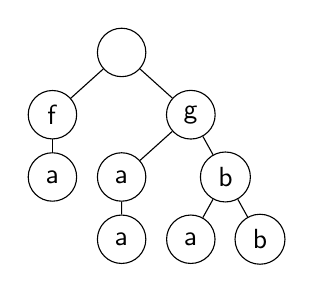
\begin{tikzpicture}[level distance=2.25em, sibling distance=5em,
%  edge from parent path={(\tikzparentnode.south) -- ++(0,-0.5em)
%   -| (\tikzchildnode.north)},
  every node/.style = {shape=circle, minimum size=1.75em, draw, align=center}]
  \node {\phantom{x}}
    child { node {$\cst{f}$}
      child { node %[fill=verylightgray]
        {$\cst{a}$} }
    }
    child { node % [fill=verylightgray]
      {$\cst{g}$}
      child { node {$\cst{a}$}
        child { node % [fill=verylightgray]
          {$\cst{a}$} }
      }
      child[sibling distance=2.5em] { node {$\cst{b}$}
        child { node %[fill=verylightgray]
          {$\cst{a}$} }
        child { node %[fill=verylightgray]
          {$\cst{b}$} }
      }
    }
    ;
\end{tikzpicture}
}}
&&
  \vcenter{\hbox{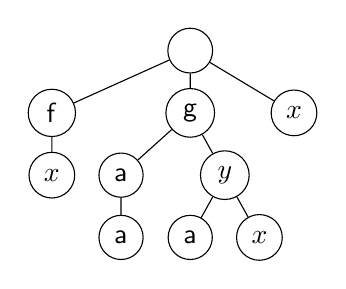
\begin{tikzpicture}[level distance=2.25em, sibling distance=5em,
%  edge from parent path={(\tikzparentnode.south) -- ++(0,-0.5em)
%   -| (\tikzchildnode.north)},
  every node/.style = {shape=circle,
    draw, align=center}]
  \node {\phantom{x}}
    child { node {$\cst{f}$}
      child { node %[fill=verylightgray]
        {$x$} }
    }
    child { node % [fill=verylightgray]
      {$\cst{g}$}
      child { node {$\cst{a}$}
        child { node % [fill=verylightgray]
          {$\cst{a}$} }
      }
      child[sibling distance=2.5em] { node {$y$}
        child { node %[fill=verylightgray]
          {$\cst{a}$} }
        child { node %[fill=verylightgray]
          {$x$} }
      }
    }
    child[sibling distance=3.75em] { node {$x$} }
    ;
\end{tikzpicture}
}}
\end{align*}
%
Assuming $\cst{a}, \cst{b}, x, y : \iota$, $\cst{f} : \iota \to \iota$,
and $\cst{g} : \iota^2 \to \iota$,
$D_1$ represents the term set
$\{
\cst{f}(\cst{a})
{,}\allowbreak\;
\cst{g}(\cst{a}, \cst{a})
{,}\allowbreak\;
\cst{g}(\cst{b}, \cst{a})
{,}\allowbreak\;
\cst{g}(\cst{b}, \cst{b})
\}$,
and $D_2$ represents the term set
$\{
\cst{f}(x)
{,}\allowbreak\;
\cst{g}(\cst{a}, \cst{a})
{,}\allowbreak\;
\cst{g}(y, \cst{a})
{,}\allowbreak\;
\cst{g}(y, x)
{,}\;
x
\}$.
%
E uses perfect discrimination trees for finding generalizations of
query terms. Thus, if the query term is
$\cst{g}(\cst{a}, \cst{a})$, it would follow the path $\cst{g}.\cst{a}.\cst{a}$
in~$D_1$ and return $\{\cst{g}(\cst{a}, \cst{a})\}.$
For~$D_2$, it would also explore paths labeled with
variables, binding them as it proceeds, and return $\{
\cst{g}(\cst{a}, \cst{a}){,}\allowbreak\; \cst{g}(y, \cst{a}){,}\allowbreak\; \cst{g}(y, x){,}\; x \}.$

It is crucial for this data structure that distinct terms always give rise to
distinct serialized terms. Conveniently, this property also holds for \lfhol{}
terms. Suppose that two distinct \lfhol{} terms yield the same serialization.
Clearly, they must disagree on parentheses; one will have the subterm $s\; t\;
u$ where the other has $s\; (t\; u).$ However, these two subterms cannot both
be well typed.

\looseness=-1
When generalizing the data structure to \lfhol, we face a complication
due to partial application. First-order terms can only be stored in leaf nodes,
but in Ehoh we must also be able to represent partially applied terms,
such as $\cst{f}$, $\cst{g}$, or $\cst{g}\;\cst{a}$ (assuming, as above, that
$\cst{f}$ is unary and $\cst{g}$ is binary). Conceptually, this can be solved
by storing a Boolean on each node indicating whether it is an accepting state.
In the implementation, the change is more subtle, because several parts of E's
code implicitly assume that only leaf nodes are accepting.

\newcommand\TermStack{\ensuremath{T}}
\newcommand\BTStack{\ensuremath{P}}

The main difficulty specific to \lfhol{} concerns applied variables. To
enumerate all generalizing terms, E needs to backtrack from child to
parent nodes. This is achieved using two stacks that store subterms of
the query term:
\TermStack{} %(\texttt{term\_\allowbreak stack})
stores the terms that
must be matched in turn against the
current subtree, and
\BTStack{} %(\texttt{term\_\allowbreak proc})
stores, for each node from
the root to the current subtree, the corresponding processed term.

Let $[a_1, \dots, a_n]$ denote an $n$-item stack with $a_1$ on top. Given a
query term $t$, the matching procedure starts at the root with $\sigma =
\emptyset$, $\TermStack{} = [t]$, and $\BTStack = []$.
%
The procedure advances by repeatedly moving to a suitable child node:
%
\begin{enumerate}
\item[A.] If the node is labeled with a symbol $\cst{f}$ and the top item
  $t$ of \TermStack{} is \confrep{}{of the form }$\cst{f}(\tuple{t}{n})$,
  replace $t$ by $n$~new items $t_1,\dots,t_n$, and push $t$ onto \BTStack.

\smallskip
\item[B.] If the node is labeled with a variable $x$, there are two subcases.
  If $x$ is already bound, check that $\sigma(x) = t$;
  otherwise, extend $\sigma$ so that $\sigma(x) = t.$ Next, pop the term $t$
  from \TermStack{} and push it onto \BTStack.
\end{enumerate}

%
The goal is to reach an accepting node. If the query term and all the terms
stored in the tree are first-order, \TermStack{} will then be empty, and the
entire query term will have been matched.
%
Backtracking works in reverse: Pop a term $t$ from \BTStack; if the current
node is labeled with an $n$-ary symbol, discard \TermStack{}'s topmost
$n$~items; push $t$ onto \TermStack. Undo any variable bindings.

As an example, looking up $\cst{g}(\cst{b}, \cst{a})$ in the tree $D_1$
would result in the following succession of stack states, starting from the
root $\varepsilon$ along the path $\cst{g}.\cst{b}.\cst{a}$:
%
\[\begin{array}{@{}l@{\kern1.5em}l@{\kern1em}l@{\kern1em}l@{\kern1em}l@{}}
& \varepsilon & \cst{g} & \cst{g}.\cst{b} & \cst{g}.\cst{b}.\cst{a} \\[.5\jot]
\sigma{:} & \emptyset & \emptyset & \emptyset & \emptyset \\
\TermStack{:} & [\cst{g}(\cst{b}, \cst{a})] & [\cst{b}, \cst{a}] & [\cst{a}] & [\,] \\
\BTStack{:} & [\,] & [\cst{g}(\cst{b}{,}\; \cst{a})] & [\cst{b}{,}\; \cst{g}(\cst{b}{,}\; \cst{a})] & [\cst{a}{,}\; \cst{b}{,}\; \cst{g}(\cst{b}, \cst{a})]
\end{array}\]
%
Backtracking amounts to moving leftward:
To get back from $\cst{g}$ to the root, we pop $\cst{g}(\cst{b}, \cst{a})$
from \BTStack, we discard two items from \TermStack{}, and we push
$\cst{g}(\cst{b}, \cst{a})$ onto \TermStack{}.

To adapt the procedure to \lfhol{}, the key idea is that an applied variable
is not very different from an applied symbol. A node labeled with an $n$-ary
head~$\zeta$ matches a prefix~$t'$ of the $k$-ary term $t$
popped from \TermStack{} and leaves $n - k$ arguments $\overline{u}$ to be
pushed back, with $t = t' \; \overline{u}.$ If $\zeta$ is a variable, it must
be bound to the prefix~$t'$ assuming $\zeta$ and $t'$ are of same type.
%
Backtracking works analogously: Given the arity $n$ of the node label $\zeta$
and the arity $k$ of the term $t$ popped from \BTStack{}, we discard the
topmost $n - k$ items $\overline{u}$ from \BTStack.

\looseness=-1
To illustrate the procedure, we consider the tree $D_2$ but change $y$'s type
to $\iota \to \iota.$ This tree stores
$\{
\cst{f}\; x
{,}\allowbreak\;
\cst{g}\; \cst{a}\; \cst{a}
{,}\allowbreak\;
\cst{g}\; (y\; \cst{a})
{,}\allowbreak\;
\cst{g}\; (y\; x)
{,}\allowbreak\;
x
\}.$
Let $\cst{g}\; (\cst{g}\;\cst{a}\;\cst{b})$ be the query term.
We have the following sequence of substitutions $\sigma$ and stacks
$\TermStack, \BTStack$:
%
\[\begin{array}{@{}l@{\kern1em}l@{\kern1em}l@{\kern1em}l@{}}
\varepsilon & \cst{g} & \cst{g}.y & \cst{g}.y.x \\[.5\jot]
\emptyset & \emptyset & \{y \mapsto \cst{g}\> \cst{a}\} & \{y \mapsto \cst{g}\> \cst{a}{,}\; x \mapsto \cst{b}\} \\[0pt]
[\cst{g}\> (\cst{g}\> \cst{a}\> \cst{b})] & [\cst{g}\> \cst{a}\> \cst{b}] & [\cst{b}] & [\,] \\[0pt]
[\,] & [\cst{g}\> (\cst{g}\> \cst{a}\> \cst{b})] & [\cst{g}\> \cst{a}\> \cst{b}{,}\;\cst{g}\> (\cst{g}\> \cst{a}\> \cst{b})] & [\cst{b}{,}\;\cst{g}\> \cst{a}\> \cst{b}{,}\;\cst{g}\> (\cst{g}\> \cst{a}\> \cst{b})]
\end{array}\]

\confrep{}{When backtracking from $\cst{g}.y$ to $\cst{g}$, by comparing
$y$'s arity of $n = 1$ with $\cst{g}\; \cst{a}\; \cst{b}$'s arity of $k = 0$,
we determine that one~item must be discarded from \TermStack{}. }%
Finally, to avoid traversing twice as many subterms as in the first-order
case, we can optimize prefixes: Given a
query term $\zeta\;\tuple{t}{n}$, we can also match prefixes
$\zeta\;\tuple{t}{k}$, where $k < n$, by allowing \TermStack{} to be nonempty when we reach an accepting node.
%If accepting nodes correspond to legal prefixes, the stack will then contain
%exactly the remaining arguments: $[t_{k+1},\dots,t_n].$

\newcommand\quadruple{\mathcalx{Q}}
Similarly to unification and matching, we present finding generalizations
in a perfect discrimination tree as a transition system. States
are quadruples $\quadruple = (\overline{t}, \overline{b}, \mathit{D}, \sigma)$, where
$\overline{t}$ is a list of terms, $\overline{b}$ is a list of tuples storing
backtracking information, $\mathit{D}$ is a discrimination
(sub)tree, and $\sigma$ is a substitution.

%With $+$ we denote list append operation, and with
%$::$ we denote operation of prepending single element to list.

Let $D$ be a perfect discrimination tree. $\Term(D)$ denotes the set of terms
stored in $D$. The function $D|_\zeta$ returns the child of $D$ labeled with
$\zeta$, if it exists. Child nodes are themselves perfect discrimination
(sub)trees. Given any node $D$, if the node is accepting, then the value stored
on that node is defined as $\mathit{val}(D) = (s, d)$, where $s$ is the
accepted term and $d$ is some arbitrary data;
%(typically, an equation whose one side is~$s$)
otherwise, $\mathit{val}(D)$ is undefined.

%We label the tree nodes using BFS, starting with 0 as label for
%root node.

%With $\mathcalx{R}$ we denote $(\overline{t}, \overline{b}, D, \sigma)$ or
%$(\mathit{v}, \sigma)$ or $\bot$.

Starting from an initial state $([t], [\,], D, \emptyset)$, where $t$ is the query
term and $D$ is an entire discrimination tree, the following transitions are
possible:
% \begin{description}[labelwidth=\widthof{\rm\textsf{AdvanceX}}]
%   \item[\rm\textsf{AdvanceF}]
%     $ ( \cst{f} \> \tuple{s}{m} \mathrel{\cdot} \overline{t}{,}\; \overline{b}{,}\; D{,}\; \sigma )
%         \Pdtarrow
%         (\tuple{s}{m} \cdot \overline{t}{,}\;
%         (\cst{f} \> \tuple{s}{m}, D, \sigma) \cdot \overline{b}{,}\; D{|}_\cst{f}{,}\; \sigma)
%       $\quad
%       if $D{|}_\cst{f}$ is defined
  
%   \smallskip
%   \item[\rm\textsf{AdvanceX}]
%     $ ( s \; \tuple{s}{m} \mathrel{\cdot} \overline{t}{,}\; \overline{b}{,}\; D{,}\; \sigma )
%         \Pdtarrow {}$ \\
%     $(\tuple{s}{m} \cdot \overline{t}{,}\; (s \; \tuple{s}{m}, D, \sigma) \cdot \overline{b}{,}\; D{|}_x{,}\; \sigma[x \mapsto s])
%       $\\
%       if $D{|}_x$ is defined, $x$ and $s$ have the same type, and
%       $\sigma(x)$ is either undefined or equal to $s$
  
%   \smallskip
%   \item[\rm\textsf{Backtrack}]
%     $ ( \tuple{s}{m} \cdot \overline{t}{,}\; (s, D_0, \sigma_0) \cdot \overline{b}{,}\; D{,}\; \sigma)
%         \Pdtarrow %\\\hphantom{\rm\textsf{AdvanceX}}%
%       (s \mathrel{\cdot} \overline{t}{,}\; \overline{b}{,}\; D_0{,}\; \sigma_0)$ \\
%       if $D_0{|}_\zeta = D$ and $m = \textit{arity}(\zeta) - \textit{arity}(s)$
  
%   \smallskip
%   \item[\rm\textsf{Success}]
%     $ ( [\,]{,}\; \overline{b}{,}\; D{,}\; \sigma )
%         \Pdtarrow (\mathit{val}(D){,}\; \sigma)$ \\
%     if~$\mathit{val}(D)$ is defined
% \end{description}

\noindent
\begin{tabular}{ll}
  \textsf{AdvanceF} & $ ( \cst{f} \> \tuple{s}{m} \mathrel{\cdot} \overline{t}{,}\; \overline{b}{,}\; D{,}\; \sigma )
           \Pdtarrow
           (\tuple{s}{m} \cdot \overline{t}{,}\;
           (\cst{f} \> \tuple{s}{m}, D, \sigma) \cdot \overline{b}{,}\; D{|}_\cst{f}{,}\; \sigma)
         $ \\
                   & if $D{|}_\cst{f}$ is defined \\[\jot]
  \textsf{AdvanceX} & $( s \; \tuple{s}{m} \mathrel{\cdot} \overline{t}{,}\; \overline{b}{,}\; D{,}\; \sigma ) 
                      \Pdtarrow {} 
                      (\tuple{s}{m} \cdot \overline{t}{,}\; (s \; \tuple{s}{m}, D, \sigma) \cdot \overline{b}{,}\; D{|}_x{,}\; \sigma[x \mapsto s])$ \\
                    & if $D{|}_x$ is defined, $x$ and $s$ have the same type,\\ & and
                    $\sigma(x)$ is either undefined or equal to $s$ \\[\jot]
  \textsf{Backtrack} & $ ( \tuple{s}{m} \cdot \overline{t}{,}\; (s, D_0, \sigma_0) \cdot \overline{b}{,}\; D{,}\; \sigma)
                      \Pdtarrow
                      (s \mathrel{\cdot} \overline{t}{,}\; \overline{b}{,}\; D_0{,}\; \sigma_0)$  \\
                      & if $D_0{|}_\zeta = D$ and $m = \textit{arity}(\zeta) - \textit{arity}(s)$ \\[\jot]
  \textsf{Success}    & $ ( [\,]{,}\; \overline{b}{,}\; D{,}\; \sigma ) \Pdtarrow (\mathit{val}(D){,}\; \sigma)$ \\
                      & if~$\mathit{val}(D)$ is defined
\end{tabular}

Above, $\cdot$ denotes prepending an element or a list to a list.
%
Intuitively, \textsf{AdvanceF} and \textsf{AdvanceX} move deeper in
the tree, generalizing cases A and B above to \lfhol{} terms.
\textsf{Backtrack} can be used to return to a previous state.
\textsf{Success} extracts the term~$t$ and data~$d$ stored in
an accepting node.

\newcommand\BDTARROW[1]{\rlap{\ensuremath{\Pdtarrow_{#1}\;}}\phantom{\Pdtarrow_\textsf{AdvanceX}\;}}

The following derivation illustrates how to locate a generalization of
$\cst{g}\; (\cst{g}\;\cst{a}\;\cst{b})$ in the tree $D_2$:\pagebreak[2]
%
\begin{align*}
 & ([\cst{g} \; (\cst{g} \; \cst{a} \; \cst{b})]{,}\;  [\,]{,}\;  D{,}\;  \emptyset) \\[-1\jot]
 \BDTARROW{\textsf{AdvanceF}}&
 ([\cst{g} \; \cst{a} \; \cst{b}]{,}\;  [(\cst{g} \; (\cst{g} \; \cst{a} \; \cst{b}), D, \emptyset)]{,}\;  D{|}_{\cst{g}}{,}\;  \emptyset)\\[-1\jot]
 \BDTARROW{\textsf{AdvanceX}}&
 ([\cst{b}]{,}\;  [(\cst{g} \; \cst{a} \; \cst{b}, D{|}_{\cst{g}}, \emptyset), \ldots]{,}\;  D{|}_{\cst{g}.y}{,}\;  \{y \mapsto \cst{g} \; \cst{a} \}) \\[-1\jot]
 \BDTARROW{\textsf{AdvanceX}}&
 ([\,]{,}\;  [(\cst{b}, D{|}_{\cst{g}.y}, \{y \mapsto \cst{g} \; \cst{a} \}), \ldots]{,}\; D{|}_{\cst{g}.y.x}{,}\; \{ y \mapsto \cst{g} \; \cst{a}{,}\; x \mapsto \cst{b} \}) \\[-1\jot]
 \BDTARROW{\textsf{Success}}& ((\cst{g} \; (y \; x), d){,}\; \{ y \mapsto \cst{g} \; \cst{a}{,}\; x \mapsto \cst{b} \})
\end{align*}

Let ${\Pdtarrow_{\mathsf{Advance}}} = {\Pdtarrow_{\mathsf{AdvanceF}}} \cup
{\Pdtarrow_{\mathsf{AdvanceX}}}$.
%and ${\Pdtarrow_{\mathsf{NoBacktrack}}} = {\Pdtarrow_{\mathsf{Advance}}} \cup
%{\Pdtarrow_{\mathsf{Success}}}$.
It is easy to show that \textsf{Backtrack} undoes an \textsf{Advance}
transition: % and can be avoided when starting from an initial state.

\begin{lemma}\label{lemma:ehoh:backtrack-inverses-advance} If $\quadruple \Pdtarrow_{\mathsf{Advance}} \quadruple'$, then
  $\quadruple' \Pdtarrow_{\mathsf{Backtrack}} \quadruple$.
  \end{lemma}
\begin{proof}
For both \textsf{Advance} steps, we show that \textsf{Backtrack} restores the state
properly. If \textsf{AdvanceF} was applied, we have
%
\begin{align*}
  ( \cst{f} \> \tuple{s}{m} \mathrel{\cdot} \overline{t}{,}\; \overline{b}{,}\; D{,}\; \sigma )
& \Pdtarrow_{\mathsf{AdvanceF}}
  (\tuple{s}{m} \cdot \overline{t}{,}\;
      (\cst{f} \> \tuple{s}{m}, D, \sigma) \cdot \overline{b}{,}\; D{|}_\cst{f}{,}\; \sigma)
\\[-\jot]
& \Pdtarrow_{\mathsf{Backtrack}}
  ( \overline{t'}{,}\; \overline{b}{,}\; D{,}\; \sigma )
\end{align*}
We must show that $\overline{t'} = \cst{f} \> \tuple{s}{m} \mathrel{\cdot} \overline{t}$.
Let $k = \textit{arity}(\cst{f})$ and $l = \textit{arity}(\cst{f} \> \tuple{s}{m})$.
By definition of $k$, we have $m = k - l$, as in \textsf{Backtrack}'s side
condition. Thus, $\overline{t'} = \cst{f} \> \tuple{s}{m} \mathrel{\cdot}
\overline{t}$. The other case is
\begin{align*}
  ( s \; \tuple{s}{m} \mathrel{\cdot} \overline{t}{,}\; \overline{b}{,}\; D{,}\; \sigma )
& \Pdtarrow_{\mathsf{AdvanceX}}
  (\tuple{s}{m} \cdot \overline{t}{,}\; (s \; \tuple{s}{m}, D, \sigma) \cdot \overline{b}{,}\; D{|}_x{,}\; \sigma')
\\[-\jot]
& \Pdtarrow_{\mathsf{Backtrack}}
  ( \overline{t'}{,}\; \overline{b}{,}\; D{,}\; \sigma )
\end{align*}
where $\sigma' = \sigma[x \mapsto s]$.
Again, we must show that $\overline{t'} = s \; \tuple{s}{m} \mathrel{\cdot} \overline{t}$. Terms
$x$ and $s$ must have the same type for \textsf{AdvanceX} to be applicable; therefore, they have the same arity. Then, we conclude $m=
\textit{arity}(s) - \textit{arity}(s \; \tuple{s}{m} ) =  \textit{arity}(x) - \textit{arity}(s \; \tuple{s}{m} )$, as in \textsf{Backtrack}'s
side condition. Thus, $\overline{t'} = s \; \tuple{s}{m} \mathrel{\cdot} \overline{t}$.
\end{proof}

\begin{lemma}\label{lemma:ehoh:advance-inverses-backtrack}
  If $\quadruple \Pdtarrow_{\mathsf{Advance}} \quadruple'
  \Pdtarrow_{\mathsf{Backtrack}} \quadruple''$, then
  $\quadruple'' = \quadruple$.
  \end{lemma}
\begin{proof}
  By Lemma~\ref{lemma:ehoh:backtrack-inverses-advance}, $\quadruple'
  \Pdtarrow_{\mathsf{Backtrack}} \quadruple$. Furthermore, \textsf{Backtrack} is
  clearly functional. Thus, $\quadruple'' = \quadruple$.
\end{proof}

\begin{lemma}\label{lemma:ehoh:backtrack-remove}
  Let $\quadruple = ([t], [\,], D, \emptyset)$. If $\quadruple
  \Pdtarrow^* \quadruple'$, then $\quadruple \Pdtarrow_{\mathsf{Advance}}^*\allowbreak
  \quadruple'$.
\end{lemma}
  
\begin{proof}
  \looseness=-1
  Let $\quadruple = \quadruple{}_{\,\,0} \Pdtarrow \cdots \Pdtarrow \quadruple{}_{\,\,n} = \quadruple'$.
  Let $i$ be the index of the first transition of the form $\quadruple{}_{\,\,i} \Pdtarrow_{\mathsf{Backtrack}}
  \quadruple{}_{\,\,i+1}$. Since $\quadruple{}_{\,\,0}$'s backtracking stack is empty, we must
  have $i \not= 0$. Hence, we have $\quadruple{}_{\,\,i-1} \Pdtarrow_{\mathsf{Advance}}
  \quadruple{}_{\,\,i} \Pdtarrow_{\mathsf{Backtrack}} \quadruple{}_{\,\,i+1}$. By
  Lemma~\ref{lemma:ehoh:advance-inverses-backtrack}, $\quadruple{}_{\,\,i-1} =
  \quadruple{}_{\,\,i+1}$. Thus, we can shorten the derivation to $\quadruple{}_{\,\,0}
  \Pdtarrow \cdots \Pdtarrow \quadruple{}_{\,\,i-1} = \quadruple{}_{\,\,i+1} \Pdtarrow
  \cdots \Pdtarrow \quadruple{}_{\,\,n}$,
  thereby eliminating one \textsf{Backtrack} transition. By repeating this
  process, we eliminate all \textsf{Backtrack} transitions.
\end{proof}

\begin{lemma}\label{lemma:ehoh:termination-pdt}
  There exist no infinite chains of the form
  $\quadruple{}_{\,\,0} \Pdtarrow_\mathsf{Advance}\allowbreak \quadruple{}_{\,\,1} \Pdtarrow_\mathsf{Advance}
  \cdots$.
\end{lemma}
\begin{proof}
  With each \textsf{Advance} transition, the height of the discrimination tree
  decreases by at least one.
\end{proof}


Perfect discrimination trees match a single term against a set of terms. To
prove them correct, we will connect them to the transition system
$\Matcharrow$ for matching (Sect.~\ref{sec:ehoh:unif-match}). This connection\pagebreak[2] will
help us show that whenever a discrimination tree stores a generalization of a
query term, this generalization can be found.
%
To express the refinement, we introduce an intermediate transition
system, $\Matchiiarrow$, that focuses on a single pair of terms (like
$\Matcharrow$) but that solves the constraints in a depth-first, left-to-right
fashion and builds the substitution incrementally (like $\Pdtarrow$).
Its initial states are of the form $([s \MATCH t], \emptyset)$. Its transitions
are as follows:

\vskip\abovedisplayskip
\noindent
\begin{tabular}{ll}
  \textsf{Decompose} & $ (\cst{f} \; \tuple{s}{m} \MATCH \cst{f} \; \tuple{t}{m} \mathrel{\cdot} \overline{c}, \, \sigma) \Matchiiarrow {} ( (s_1 \MATCH t_1, \ldots, s_m \MATCH t_m) \cdot \overline{c}, \sigma ) $ \\[\jot]
  \textsf{DecomposeX} & $(x \; \tuple{s}{{m}} \MATCH u \; \tuple{t}{{m}} \mathrel{\cdot} \overline{c}, \, \sigma) \Matchiiarrow {} ( (s_1 \MATCH t_1, \ldots, s_m \MATCH t_m) \cdot \overline{c}, \sigma[x \mapsto u] )$ \\
                    & if $x$ and $u$ have the same type and either $\sigma(x)$ is undefined or $\sigma(x)=u$ \\[\jot]
  \textsf{Success} & $ ([\,], \, \sigma) \Matchiiarrow  \sigma $ \\[\jot]
  \textsf{Clash}    & $ (\cst{f} \; \tuple{s}{m} \MATCH \cst{g} \; \tuple{t}{n} \mathrel{\cdot} \overline{c}, \, \sigma) \Matchiiarrow \bot $ \\[\jot]
  \textsf{ClashTypeX}    & $(x \; \tuple{s}{{m}} \MATCH u \; \tuple{t}{{m}} \mathrel{\cdot} \overline{c}, \, \sigma) \Matchiiarrow \bot$ \\
                         & if~$x$ and $u$ have different types  \\[\jot]
  \textsf{ClashLenXF}    & $(x \; \tuple{s}{{m}} \MATCH \cst{f} \; \tuple{t}{{n}} \mathrel{\cdot} \overline{c}, \, \sigma) \Matchiiarrow \bot$ \\
                         & if~$m > n$  \\[\jot]
  \textsf{ClashLenXY}    & $(x \; \tuple{s}{{m}} \MATCH y \; \tuple{t}{{n}} \mathrel{\cdot} \overline{c}, \, \sigma) \Matchiiarrow \bot$ \\
                         & if~$x \neq y$ and $m > n$ \\[\jot]
  \textsf{ClashFX}    & $(\cst{f} \; \overline{s} \MATCH x \; \overline{t}  \mathrel{\cdot} \overline{c}, \, \sigma) \Matchiiarrow \bot$ \\[\jot]
  \textsf{Double}    & $(x \; \tuple{s}{{m}} \MATCH u \; \tuple{t}{{m}}  \mathrel{\cdot} \overline{c}, \, \sigma) \Matchiiarrow \bot$ \\
                     & if $x$ and $u$ have the same type, $\sigma(x)$ is defined, and $\sigma(x) \neq u$ \\[\jot]
\end{tabular}
\vskip\belowdisplayskip
\newcommand\AlphaMatch[1]{\alpha(#1)}
We need an auxiliary function to convert $\Matchiiarrow$ states to
$\Matcharrow$ states.
Let
$\AlphaMatch{\{ x_1 \mapsto s_1,\allowbreak \ldots, x_m \mapsto s_m \}}
 = \{ x_1 \MATCH s_1,\ldots,\,\allowbreak x_m \MATCH s_m \}$,
$\AlphaMatch{\overline{c}, \sigma} =
\{ c \mid c \in \overline{c} \} \mathrel\cup \AlphaMatch{\sigma}$, and
$\AlphaMatch{\bot} = \bot$.
%
Moreover, let $\mathcal{S}$ range over states of the form $(\overline{c}, \sigma)$ and
$\mathcalx{R}$ additionally range over special states of the form $\sigma$ or
$\bot$.


\begin{lemma}\label{lemma:ehoh:match-refinement}
  If $\mathcal{S} \Matchiiarrow \mathcalx{R}$,
  then $\AlphaMatch{\mathcal{S}} \Matcharrow^* \AlphaMatch{\mathcalx{R}}$.
\end{lemma}
\begin{proof}
By case distinction on $\mathcalx{R}$. Let $\mathcal{S} = (\overline{c}, \sigma)$.

\medskip

\begin{sloppypar}%
  \noindent
  \textsc{Case} $\mathcalx{R} = (\overline{c'}, \sigma')$:\enskip
  Only $\Matchiiarrow_{\mathsf{Decompose}}$ and
  $\Matchiiarrow_{\mathsf{DecomposeX}}$ are possible.
  If $\Matchiiarrow_{\mathsf{Decompose}}$ is applied, then $\Matcharrow_{\mathsf{Decompose}}$
  is applicable and results in $\AlphaMatch{\mathcalx{R}}$.
  If $\Matchiiarrow_{\mathsf{DecomposeX}}$ is applied,
  we have either $m>0$, and $\Matcharrow_{\mathsf{DecomposeX}}$ is applicable,
  or $m = 0$, and $\AlphaMatch{\overline{c'},\sigma'} = \AlphaMatch{\mathcal{S}}$,
  which implies that the two states are connected by an idle transition of
  $\Matcharrow^*$.
  \end{sloppypar}
  
  \medskip
  
  \noindent
  \textsc{Case} $\mathcalx{R} = \bot$:\enskip
  All the $\Matchiiarrow$ rules resulting in $\bot$ except for \textsf{Double}
  have the same side conditions as the corresponding $\Matcharrow$ rules.
  $\Matchiiarrow_{\mathsf{Double}}$ corresponds to
  $\Matcharrow_{\mathsf{Double}}$ if $m=0$. If $m \neq 0$, we need
  an intermediate $\Matcharrow_{\mathsf{DecomposeX}}$ step before
  $\Matcharrow_{\mathsf{Double}}$ can be applied to derive $\bot$. Since
  $\Matchiiarrow_{\mathsf{Double}}$ is applicable, $\sigma(x) = u'
  \neq u$. Hence, $x \MATCH u'$ must be present in $\AlphaMatch{\overline{c},
  \sigma}$. $\Matcharrow_{\mathsf{DecomposeX}}$ will augment this set with
  $x \MATCH u$, enabling $\Matcharrow_{\mathsf{Double}}$.
  
  \medskip
  
  \noindent
  \textsc{Case} $\mathcalx{R} = \sigma$:\enskip
  The only possible rule is $\Matchiiarrow_{\mathsf{Success}}$,
  with $\overline{c}=[\,]$. Since $\AlphaMatch{\mathcal{S}} = \AlphaMatch{\sigma}$,
  this transition corresponds to an idle transition of $\Matcharrow^*$.
\end{proof}

\begin{lemma}\label{lemma:ehoh:refined-match-partial-correctness}\,%
  If $\mathcal{S} \Matchiiarrow^{!} \mathcalx{R}$, then $\mathcalx{R}$ is either
  some substitution $\sigma'$ or $\bot$.
  If $\mathcal{S} \Matchiiarrow^{!} \sigma'$, then $\sigma'$ is the MGG
  of~$\AlphaMatch{\mathcal{S}}$.
  If $\mathcal{S} \Matchiiarrow^{!} \bot$, then $\AlphaMatch{\mathcal{S}}$ has
  no solutions.
  \end{lemma}
\begin{proof}
  %Let $\mathcal{S} = (\overline{c}, \sigma)$.
  
  First, we show that states $\mathcal{S}' = (\overline{c'}, \sigma')$ cannot be
  normal forms, by exhibiting transitions from such states. If $\overline{c'} =
  [\,]$, the $\Matchiiarrow_{\mathsf{Success}}$ rule would apply. Otherwise, let
  $\overline{c'} = c_1 \cdot \overline{c''}$ and consider the matching problem
  $\{c_1\} \cup \AlphaMatch{\sigma'}$. If this problem is in solved form, $c_1$
  is a constraint corresponding to a solved variable, and we can apply
  $\Matchiiarrow_{\mathsf{DecomposeX}}$ to move the constraint into the
  substitution. Otherwise, some $\Matcharrow$ rule can be applied. It
  necessarily focuses on $c_1$, since the constraints from
  $\AlphaMatch{\sigma'}$ correspond to solved variables. In all cases except for
  $\Matcharrow_{\mathsf{DecomposeX}}$, a homologous
  $\Matchiiarrow$ rule  can be applied to $\mathcal{S}'$. If $\Matcharrow_{\mathsf{DecomposeX}}$
  would make $\Matcharrow_{\mathsf{Double}}$ applicable, then we can apply $\Matchiiarrow_{\mathsf{Double}}$ to $\mathcal{S}'$;
  otherwise, $\Matchiiarrow_{\mathsf{DecomposeX}}$ is applicable.
  
  Second, by Lemma \ref{lemma:ehoh:match-refinement},
  if $\mathcal{S} \Matchiiarrow^{!} \sigma'$, then
  $\AlphaMatch{\mathcal{S}} \Matcharrow^* \AlphaMatch{\sigma'}$.
  By construction, $\AlphaMatch{\sigma'}$ is in solved form.
  Therefore, $\AlphaMatch{\mathcal{S}} \Matcharrow^{!} \AlphaMatch{\sigma'}$.
  By completeness of $\Matcharrow$, the substitution corresponding to
  $\AlphaMatch{\sigma'}$---that is, $\sigma'$---is the MGG of~$\AlphaMatch{\mathcal{S}}$.
  
  Third, by Lemma~\ref{lemma:ehoh:match-refinement}, if $\mathcal{S}
  \Matchiiarrow^{!} \bot$, then $\AlphaMatch{\mathcal{S}} \Matcharrow^{!} \bot$.
  By soundness of $\Matcharrow$, $\AlphaMatch{\mathcal{S}}$ has
  no solutions.
\end{proof}


\begin{lemma}\label{lemma:ehoh:refined-match-termination}\,%
  The relation $\Matchiiarrow$ is well founded.
  \end{lemma}
\begin{proof}
  By Lemma \ref{lemma:ehoh:match-refinement}, every $\Matchiiarrow$ transition
  corresponds to zero or more $\Matcharrow$ transitions.
  Since $\Matcharrow$ is well founded,
  the only transitions that can violate well-foundedness of $\Matchiiarrow$ are
  the ones that take idle $\Matcharrow^*$ transitions:
  $\Matchiiarrow_{\mathsf{DecomposeX}}$ for $m=0$ and
  $\Matchiiarrow_{\mathsf{Success}}$. The latter is terminal, so it cannot
  contribute to infinite chains.
  As for $\Matchiiarrow_{\mathsf{DecomposeX}}$, with $m=0$,
  it decreases the following measure~$\mu$, which the other rules nonstrictly
  decrease, with respect to the multiset extension of $<$ on natural numbers:
  $\mu([s_1 \MATCH t_1, \ldots, s_m \MATCH t_m], \sigma) =
    \{\left|s_1\right|, \ldots \left|s_m\right|\}$,
  where $\left|s\right|$ denotes the syntactic size of $s$.
\end{proof}
  
\begin{lemma}\label{lemma:ehoh:refined-matching-solution}
  If term $s$ generalizes $t$, then $([s \MATCH t], \emptyset) \Matchiiarrow^! \sigma$,
  where $\sigma$ is the MGG of $s \MATCH t$.
\end{lemma}
\begin{proof}
By Lemma \ref{lemma:ehoh:refined-match-termination}, there exists a normal form
$\mathcalx{R}$ starting from $\mathcal{S} = ([s \MATCH t],\allowbreak \emptyset)$. Since $s
\MATCH t$ is solvable, by Lemma~\ref{lemma:ehoh:refined-match-partial-correctness},
and soundness of $\Matchiiarrow$ (a consequence of Lemma \ref{lemma:ehoh:match-refinement}
and soundness of $\Matcharrow$),
$\mathcalx{R}$ must be the MGG for $s$ and~$t$.
\end{proof}


\begin{lemma}\label{lemma:ehoh:pdt-complete-help}
  If there exists a term $s \in \Term(D)$ that generalizes the query term~$t$,
  then there exists a derivation $([t], [\,],\allowbreak D,\allowbreak \emptyset) \Pdtarrow^! ((s, d),
  \sigma)$. %, where $\sigma$ is the MGG for $s$ and $t$.
  \end{lemma}
  \begin{proof}
    By Lemma \ref{lemma:ehoh:refined-matching-solution}, we know that $(s \MATCH t,
    \emptyset) \Matchiiarrow^! \sigma$ for each $s \in \Term(D)$ generalizing $t$.
    This means that there exists a derivation
    $([s \MATCH t], \emptyset) = (\overline{c_0}, \sigma_0) \Matchiiarrow \cdots \Matchiiarrow (\overline{c_n}, \sigma_n)\allowbreak \Matchiiarrow \sigma$.
    The $n$ first transitions must be \textsf{Decompose} or \textsf{DecomposeX},
    and the last transition must be \textsf{Success}.

    We show that there exists a derivation of the form
    $([t], [\,],\allowbreak D, \emptyset) = \quadruple{}_{\,\,0}\allowbreak \Pdtarrow \cdots
    \Pdtarrow \quadruple{}_{\,\,n} \Pdtarrow ((s, d),\sigma)$, where $\quadruple{}_{\,\,i} =
    (\overline{t_i}, \overline{b_i}, \allowbreak D_i, \sigma_i)$ for each $i$.
  %
    We define $\overline{t_i}$, $\overline{b_i}$, and $D_i$ as follows, for $i > 0$.
    The list $\overline{t_i}$ consists of the right-hand sides of the
    constraints~$\overline{c_i}$, in the same order.
    %todo:
    Let $\mathit{hd}$ be the function that extracts the head of a list. We set
          $b_i = (\mathit{hd}(\overline{t_{i-1}}),\allowbreak D_{i-1}, \sigma_{i-1})$. We know that $\overline{c_{i-1}}$ is
          nonempty, since there exists a transition $(\overline{c_{i-1}}, \sigma_{i-1}) \Matchiiarrow (\overline{c_i}, \sigma_i)$%
          ; thus, $\overline{t_{i-1}}$ is nonempty.
    If an accepting node storing~$s$ was reached in $n$~steps, the
      serialization of $s$ must be of the form $\zeta_1.\cdots.\zeta_n$. Take $D_i
      = D_{i-1}{|}_{\zeta_i}$.
  
    The sequence of states $\quadruple{}_{\,\,i}$ forms a
    derivation:
    If $(\overline{c_i},\allowbreak \sigma_i)\allowbreak \Matchiiarrow_\textsf{Decompose}
    (\tuple{c}{{i+1}},\allowbreak \sigma_{i+1})$, then $\quadruple{}_{\,\,i}
    \Pdtarrow_\textsf{AdvanceF} \allowbreak \quadruple{}_{\,\,i+1}$.
    If $(\overline{c_i},\allowbreak \sigma_i) \Matchiiarrow_\textsf{DecomposeX}
    (\tuple{c}{{i+1}},\allowbreak \sigma_{i+1})$, then $\quadruple{}_{\,\,i}
    \Pdtarrow_\textsf{AdvanceX} \quadruple{}_{\,\,i+1}$.
    If $(\overline{c_n},\allowbreak \sigma_n) \Matchiiarrow_\textsf{Success} \sigma$, then
    $\quadruple{}_{\,\,n} \Pdtarrow_\textsf{Success} ((s, d),\allowbreak \sigma)$.
\end{proof}
  
\begin{lemma}\label{lemma:ehoh:pdt-soundi}
  If $([t], [\,], D, \emptyset) \Pdtarrow^+ ((s, d), \sigma)$, then $s \in \Term(D)$
  and $\sigma$ is the MGG of $s \MATCH t$.
  \end{lemma}
  
  \begin{proof}
  Let $([t], [\,], D, \emptyset) =
  \quadruple{}_{\,\,0} \Pdtarrow \cdots \Pdtarrow \quadruple{}_{\,\,n}
  \Pdtarrow ((s, d), \sigma)$ be a derivation, where $\quadruple{}_{\,\,i} =
  (\overline{t_i}, \overline{b_i},\allowbreak D_i, \sigma_i)$ for each $i$. Without loss of
  generality, by Lemma \ref{lemma:ehoh:backtrack-remove}, we can assume that the
  derivation contains no \textsf{Backtrack} transitions.
  
  The first conjunct, $s \in \Term(D)$, clearly holds
  %by definition --- some invariant must be needed here
  for any term found
  from an initial state. To prove the second conjunct, we first introduce a
  function $\mathit{preord}$ that defines the preorder decomposition of a list
  of terms:
  $\mathit{preord}([\,]) = [\,]$ and
  $\mathit{preord}(\zeta \; \tuple{s}{n} \cdot \overline{xs}) =
  (\zeta{,}\; \tuple{s}{n} \cdot \overline{xs}) \cdot \mathit{preord}(\tuple{s}{n} \cdot \overline{xs})$.
  %
  Given a term~$s$, $\mathit{preord}([s])$ gives a sequence
  $(\zeta_1, \tuple{u}{1}), \dots, \allowbreak
  (\zeta_n, \tuple{u}{n})$.
  Since $s \in \Term(D)$,
  the sequence $D_0, \ldots, D_n$ follows the preorder serialization of $s$:
  $D_i = D_{i-1}|_{\zeta_i}$ for $i > 0$.
  
  Next, we show that there exists a derivation of the form
  $([s \MATCH t], \emptyset) = \mathcal{S}_0 \Matchiiarrow
  \cdots \Matchiiarrow \mathcal{S}_n \Matchiiarrow \sigma$, where
  $\mathcal{S}_i = (\overline{c_i}, \sigma_i)$. We define $\overline{c_i}$, for $i>0$,
  as the list of constraints whose left-hand sides are the elements of $\overline{u_i}$
  and right-hand sides are the elements of $\overline{t_i}$, in the order they appear in the respective lists.
  By inspecting the definition of $\mathit{preord}$
  and the changes each \textsf{Advance} step makes
  to the head of $\overline{t_i}$, we can see that $\overline{u_i}$ and $\overline{t_i}$  have the same length.
  The sequence of states $\mathcal{S}_i$ forms a derivation:
  %
  If $\quadruple{}_{\,\,i} \Pdtarrow_\textsf{AdvanceF} \quadruple{}_{\,\,i+1}$, then $\mathcal{S}_i \Matchiiarrow_\textsf{Decompose} \mathcal{S}_{i+1}$.
  If $\quadruple{}_{\,\,i} \Pdtarrow_\textsf{AdvanceX} \quadruple{}_{\,\,i+1}$, then $\mathcal{S}_i\allowbreak \Matchiiarrow_\textsf{DecomposeX} \mathcal{S}_{i+1}$.
  If $\quadruple{}_{\,\,n} \Pdtarrow_\textsf{Success} \sigma$, then
  $\mathcal{S}_n\allowbreak \Matchiiarrow_\textsf{Success} \sigma$.
\end{proof}
  
\begin{theorem}[Total Correctness]\label{theorem:ehoh:pdt-complete}\,%
  Let $D$ be a perfect discrimination tree and $t$ be a term.
  The sets $\{ s \in \Term(D) \mid \exists \sigma.\; \sigma(s) = t \}$
  and $\{ s \mid \exists d, \sigma.\; ([t], [\,], D, \emptyset) \allowbreak
  \Pdtarrow^! ((s, d), \sigma) \}$ are equal.
\end{theorem}
\begin{proof}
  This follows from Lemmas \ref{lemma:ehoh:pdt-complete-help} and \ref{lemma:ehoh:pdt-soundi}.
\end{proof}

The theorem tells us that given a term~$t$, all generalizations $s$ stored
in the perfect discrimination tree can be found, but it does not exclude
nondeterminism. Often, both \textsf{AdvanceF} and \textsf{AdvanceX} are
applicable. To find all generalizations, we need to follow both transitions.
But for some applications, it is enough to find a single generalization.

To cater for both types of applications, E provides iterators that store the
state of a traversal. After an iterator is initialized
with the root node $D$ and the query term $t$, each call to
\textsc{FindNextVal} will move the iterator to the next node that generalizes
the query term and stores a value, indicating an accepting node. After all
such nodes have been traversed, the iterator is set to point to
$\mathit{Null}$.

The following definitions constitute the high-level interface for
iterating through values incrementally or for obtaining all values of nodes that
store generalizations of the query term in $D$.


\begin{quotex}
  \MyFunction{InitIter}{PDTNode $D$, Term $t$}
  \q $i \gets \textsc{Iterator}()$ \\
  \q $(i.\mathit{node}, i.\mathit{t\_stack}, i.\mathit{t\_proc}, i.\mathit{c\_iter}) \gets (D, [t], [\,], \textit{Start})$ \\
  \q \MyReturn $i$
  
  \vskip 1.5\jot
  
  \MyProcedure{FindNextVal}{Iterator $i$}
  \q \MyDo
  \qq \textsc{FindNextNode}($i$) \\
  \q \MyWhileOfDo{$i.\mathit{node} \not= \mathit{Null} \mathrel\land
    \\ \qqq  (\lnot\, i.\mathit{t\_stack}.\mathit{isEmpty}()
    \mathrel\lor \lnot\, i.\mathit{node}.\mathit{has\_val}())$}
  
  \vskip 1.5\jot
  
  \MyFunction{AllVals}{PDTNode $D$, Term $t$}
  \q $\mathit{i} \gets \textsc{InitIter}(D, t)$ \\
  \q $\textsc{FindNextVal}(i)$ \\
  \q $\mathit{res} \gets \emptyset$ \\
  \q \MyWhile{$\mathit{i.node} \neq \mathit{Null}$}
  \qq $\mathit{res} \gets \mathit{res} \cup \{ \mathit{i.node.val()} \}$ \\
  \qq $\textsc{FindNextVal}(i)$
  \\[\jot]
  \q \MyReturn $\mathit{res}$
  \end{quotex}
  
  The core functionality is implemented in \textsc{FindNext\-Node}, presented below. This
  procedure moves the iterator to the next node that has not been explored in the
  search for generalization, or \textit{Null} if the entire tree has been
  traversed. It first goes through all child nodes labeled with a variable before
  possibly visiting the child node labeled with a function symbol. We assume that
  we can iterate through the children of a node using a function
  \textsc{NextVarChild} that, given a tree node and iterator through children,
  advances the iterator to the child representing the next variable. Furthermore, we
  assume that the iterator can also be in the distinguished states \textit{Start}
  and \textit{End}.
  \textit{Start} indicates that no child has been visited yet; \textit{End}
  indicates that we have visited all children. Finally, the expression
  $n.\mathit{child}(\zeta)$ returns a child of the node $n$ labeled $\zeta$ if
  such a child exists or $\mathit{Null}$ otherwise.
  
  \begin{quotex}
  \MyProcedure{FindNextNode}{Iterator $i$}
  \q \MyIf{$i.\mathit{t\_stack.isEmpty}()$}
  \qq \textsc{BacktrackToVar}($i$)
  \\[\jot]
  \q $\mathit{advanced} \gets \mathit{False}$ \\
  \q \MyWhile{$i.\mathit{node} \neq \mathit{Null} \mathrel\land \lnot\, \mathit{advanced}$}
  %\qq \MyIf{$i.\mathit{c\_iter} < \textit{End}$}
  \qq \MyWhile{$i.\mathit{c\_iter} \neq \textit{End} \mathrel\land \lnot\, \mathit{advanced}$}
  \qqq $i.\mathit{c\_iter} \gets \textsc{NextVarChild}(i.\mathit{node}, i.\mathit{c\_iter})$ \\
  \qqq \MyIf{$i.\mathit{c\_iter} \neq \textit{End}$}
  \qqqq $x \gets i.\mathit{c\_iter}.\mathit{var}()$ \\
  \qqqq $t \gets i.\mathit{t\_stack}.\mathit{top}()$ \\
  \qqqq $\mathit{s} \gets \textsc{GobblePrefix}(x, t)$ \\
  \qqqq \MyIf{$\mathit{s} \neq \mathit{Null} \mathrel\land \\ \qqqqqq
                (x.\mathit{binding} = \mathit{Null} \mathrel\lor x.\mathit{binding} = \mathit{s})$}
  \qqqqq $i.\mathit{t\_stack}.\mathit{pop}()$ \\
  \qqqqq \MyForDownto{$j \gets t.\mathit{num\_args}$\\\qqqqqqq\ignorespaces}{$\mathit{s}.\mathit{num\_args}+1$}
  \qqqqqq $i.\mathit{t\_stack}.\mathit{push}(t.\mathit{args}[j])$ \\
  \qqqqq \MyIf{$x.\mathit{binding} = \mathit{Null}$}
  \qqqqqq $x.\mathit{binding} \gets \mathit{s}$ \\
  \qqqqqq $i.\mathit{t\_proc}.\mathit{push}
                      ( (t, i.\mathit{node}, i.\mathit{c\_iter}, \mathit{True} ) )$ \\
  \qqqqq \MyElse
  \qqqqqq $i.\mathit{t\_proc}.\mathit{push}
                      ( (t, i.\mathit{node}, i.\mathit{c\_iter}, \mathit{False}) )$
  \\[\jot]
  \qqqqq $ \mathit{i.\mathit{node}} \gets i.\mathit{node}.child(x)$ \\
  \qqqqq $ \mathit{advanced} \gets \mathit{True}$
  \\[\jot]
  \qq $t \gets i.\mathit{t\_stack}.\mathit{top}()$ \\
  \qq \MyIf{$i.\mathit{c\_iter} = \textit{End} \mathrel\land
          \lnot\, t.\mathit{head}.\mathit{isVar}()  \\ \qqq \mathrel\land
          D.\mathit{child}(t.\mathit{head}) \neq \mathit{Null}$}
  \qqq $i.\mathit{t\_stack}.\mathit{pop}()$ \\
  \qqq \MyForDownto{$j \gets t.\mathit{num\_args}$}{$1$}
  \qqqq $i.\mathit{t\_stack}.\mathit{push}(t.\mathit{args}[j])$ \\
  \qqq $i.\mathit{t\_proc}.\mathit{push}
              ( (t, i.\mathit{node}, \mathit{End}, \mathit{False}) )$ \\
  \qqq $\mathit{i.\mathit{node}} \gets i.\mathit{node}.\mathit{child}(t.\mathit{head})$ \\
  \qqq $\mathit{advanced} \gets \mathit{True}$
  \\[\jot]
  \qq \MyIf{$\lnot\, \mathit{advanced}$}
  \qqq \textsc{BacktrackToVar}$(i)$ \\
  \qq \MyElse
  \qqq $i.\mathit{c\_iter} \gets \textit{Start}$
  
  \vskip 2\jot
  
  \MyProcedure{BacktrackToVar}{Iterator $i$}
  \q \MyForever
  \qq \MyIf{$i.\mathit{t\_proc}.\mathit{isEmpty}()$}
  \qqq $i.\mathit{node} \gets \mathit{Null}$ \\
  \qqq \MyReturn \\
  \qq \MyElse
  \qqq $(t, D, \mathit{c\_iter}, \mathit{var\_unbound}) \gets i.\mathit{t\_proc}.\mathit{pop}()$ \\
  \qqq $\mathit{label\_arity} \gets i.\mathit{node}.\mathit{label}.\mathit{type}.\mathit{arity}$ \\
  \qqq $\mathit{t\_arity} \gets t.\mathit{type}.\mathit{arity}$
  \\[\jot]
  \qqq \MyForTo{$i \gets 1$}{$\mathit{label\_arity} - \mathit{t\_arity}$}
  \qqqq $i.\mathit{t\_stack}.\mathit{pop}()$
  \\[\jot]
  \qqq $i.\mathit{t\_stack}.\mathit{push}(t)$ \\
  \qqq $i.\mathit{node} \gets D$ \\
  \qqq $i.\mathit{c\_iter} \gets \mathit{c\_iter}$
  \\[\jot]
  \qqq \MyIf{$\mathit{var\_unbound}$}
  \qqqq $i.\mathit{node}.\mathit{label}.\mathit{binding} \gets \mathit{Null}$
  \\[\jot]
  \qqq \MyIf{$\mathit{c\_iter} \neq\textit{End}$}
  \qqqq \MyReturn
  \end{quotex}
  
The pseudocode uses a slightly different representation of backtracking tuples
than ${\Pdtarrow}$. In the \textsf{AdvanceX} rule,
$\sigma$ changes only if the variable~$x$ was previously not bound.
Instead of creating and storing substitutions explicitly, we simply remember
whether the variable was bound in this step or not, in the
$\mathit{var\_unbound}$ tuple component. Then we rely on the label~$x$ of the
current node and its \textit{binding} field to carry the substitutions.
Similarly, since our strategy is to traverse the tree by first visiting the
variable-labeled child nodes, we need to remember how far we have come with
this traversal. We store this information in the $\mathit{c\_iter}$ tuple
component.

\subsection{Fingerprint Indices}
\looseness=-1
Fingerprint indices \cite{ss-12-fp-indexing} trade perfect indexing for
a compact memory representation and more flexible retrieval conditions.
The basic idea is to compare terms by looking only at a few
predefined sample positions. If we know that term $s$ has
symbol $\cst{f}$ at the head of the subterm at~2.1 and term $t$ has
$\cst{g}$ at the same position, we can immediately conclude that $s$ and $t$
are not unifiable.

% They are
% based on the idea that when one samples a term position only the following
% situations may happen: position corresponds to
% a variable or a complex term; position is invalid---but under some substitution it
% can become valid; position is invalid and no substitution makes it valid.

Let $\AA$ (``at a variable''),
$\BB$ (``below a variable''), and
$\NN$ (``nonexistent'') be distinguished symbols\begin{rep}
not present in the signature, and let $q < p$ denote that position $q$ is a proper prefix of $p$\end{rep}
(e.g., $\varepsilon < 2 < 2.1$). Given a term $t$ and a position~$p$, the
\emph{fingerprint function} $\Gfpf$ is defined as
\[
  \Gfpf(t,p) =
  \begin{cases}
    \cst{f} & \text{if $t|_p$ has a symbol head $\cst{f}$} \\[-\jot]
    \AA & \text{if $t|_p$ is a variable} \\[-\jot]
    \BB & \text{if $t|_q$ is a variable for some $q < p$} \\[-\jot]
    \NN & \text{otherwise}
  \end{cases}
\]

Based on a fixed tuple of positions $\tuple{p}{n}$,
the \emph{fingerprint} of a term $t$ is defined as
$\mathit\Fp(t) = \bigl(\Gfpf(t, p_1), \ldots, \Gfpf(t, p_n)\bigr).$ To compare
two terms $s$ and $t$, it suffices to check that their fingerprints are
componentwise compatible using the following unification and matching
matrices, respectively:
%
\newcolumntype{L}[1]{>{\raggedright\let\newline\\\arraybackslash\hspace{0pt}}m{#1}}
\newcolumntype{C}[1]{>{\centering\let\newline\\\arraybackslash\hspace{0pt}}m{#1}}
\newcolumntype{R}[1]{>{\raggedleft\let\newline\\\arraybackslash\hspace{0pt}}m{#1}}

\confrep{
\begin{align*}
& \hbox{\begin{tabular}{@{}C{0.75em}|C{0.75em}C{0.75em}C{0.75em}C{0.75em}C{0.75em}@{}}
& $\cst{f}_1$ & $\cst{f}_2$ & \AA & \BB & \NN \\
\hline
$\cst{f}_1\vphantom{^{()}}$ & & \xmark & & & \xmark \\
\AA & & & & & \xmark \\
\BB & & & & & \\
\NN & \xmark & \xmark & \xmark & &
\end{tabular}}
&
& \hbox{\begin{tabular}{@{}C{0.75em}|C{0.75em}C{0.75em}C{0.75em}C{0.75em}C{0.75em}@{}}
& $\cst{f}_1$ & $\cst{f}_2$ & \AA & \BB & \NN \\
\hline
$\cst{f}_1\vphantom{^{()}}$ & & \xmark & \xmark & \xmark & \xmark \\
\AA & & & & \xmark & \xmark \\
\BB & & & & & \\
\NN & \xmark & \xmark & \xmark & \xmark &
\end{tabular}}
\end{align*}
}{
\begin{align*}
& \hbox{\begin{tabular}{@{}C{0.75em}|C{0.75em}C{0.75em}C{0.75em}C{0.75em}C{0.75em}@{}}
& $\cst{f}_1$ & $\cst{f}_2$ & \AA & \BB & \NN \\
\hline
$\cst{f}_1\vphantom{^{()}}$ & & \xmark & & & \xmark \\
$\cst{f}_2$ & \xmark & & & & \xmark \\
\AA & & & & & \xmark \\
\BB & & & & & \\
\NN & \xmark & \xmark & \xmark & &
\end{tabular}}
&
& \hbox{\begin{tabular}{@{}C{0.75em}|C{0.75em}C{0.75em}C{0.75em}C{0.75em}C{0.75em}@{}}
& $\cst{f}_1$ & $\cst{f}_2$ & \AA & \BB & \NN \\
\hline
$\cst{f}_1\vphantom{^{()}}$ & & \xmark & \xmark & \xmark & \xmark \\
$\cst{f}_2$ & \xmark & & \xmark & \xmark & \xmark \\
\AA & & & & \xmark & \xmark \\
\BB & & & & & \\
\NN & \xmark & \xmark & \xmark & \xmark &
\end{tabular}}
\end{align*}
}%
%
The rows and columns correspond to $s$ and $t$, respectively. The
metavariables $\cst{f}_1$~and~$\cst{f}_2$ represent arbitrary distinct symbols.
Incompatibility is indicated by $\xmark{}$.

\newcommand\fpok{\text{--}}

As an example,
let $(\varepsilon, 1,\allowbreak 2,\allowbreak 1.1,\allowbreak 1.2,\allowbreak 2.1, 2.2)$
be the sample positions,
and let $s = \cst{f}(\cst{a}, x)$ and $t = \cst{f}(\cst{g}(x), \cst{g}(\cst{a}))$
be the terms to unify. Their fingerprints are
$\Fp(s) = (\cst{f}, \cst{a}, \AA, \NN, \NN,\allowbreak \BB, \BB)$
and
$\Fp(t) = (\cst{f}, \cst{g}, \cst{g}, \AA, \NN, \cst{a}, \NN)$.
%
Using the left matrix, we compute the compatibility vector
%
$(\fpok, \xmark, \fpok, \xmark, \fpok, \fpok, \fpok).$
%
The mismatches at positions 1 and 1.1 indicate that $s$ and $t$ are not unifiable.

A fingerprint index is a trie that stores a term set $T$ keyed by fingerprint.
The term $\cst{f}(\cst{g}(x), \cst{g}(\cst{a}))$ above would
be stored in the node addressed by
$\cst{f}.\cst{g}.\cst{g}.\AA.\NN.\cst{a}.\NN$, together with other
terms that share the same fingerprint.
This scheme makes it possible to unify or match a query term $s$
against all the terms $T$ in one traversal. Once a node storing the terms $U
\subseteq T$ has been reached, due to overapproximation we must apply
unification or matching on $s$ and each $u \in U.$ % to obtain correct results.

When adapting this data structure to \lfhol{}, we must first choose a
suitable notion of position in a term. Conventionally, higher-order
positions are strings over $\{1, 2\}$, but this is not graceful.
% indicating, for each binary
% application $t_1\;t_2$, which term $t_i$ to follow.
Instead, it is preferable to generalize the first-order notion to
flattened \lfhol{} terms---e.g.,
$x\> \cst{a} \> \cst{b} \> |_{1} = \cst{a}$
and $x\> \cst{a} \> \cst{b} \> |_{2} = \cst{b}.$
%
However, this approach fails on applied variables. For example,
although $x \> \cst{b}$ and $\cst{f} \> \cst{a} \> \cst{b}$ are
unifiable (using $\{ x \mapsto \cst{f} \> \cst{a} \}$), sampling position 1
would yield a clash between
$\cst{b}$~and~$\cst{a}.$ To ensure that positions remain stable under
substitution, we propose to number arguments in reverse:
$t {|}^\varepsilon = t$ and
$\zeta \> t_n \, \ldots \, t_1  |^{i.p} = t_{i} |^p$
if $1 \le i \le n$.
We use a nonstandard notation, $t|^p$, for this nonstandard
notion. The operation is undefined for out-of-bound indices.

\begin{lemma}\label{lemma:fpindex-aux}
  Let $s$ and $t$ be unifiable terms, and let $p$ be a position such that the
  subterms $s|^{p}$ and $t|^{p}$ are defined. Then $s|^{p}$ and $t|^{p}$ are
  unifiable.
\end{lemma}
\begin{proof}
  By structural induction on $p$. The case $p = \varepsilon$ is trivial.

  \medskip

  \noindent
  \textsc{Case $p = q.i$}:\enskip
  Let $s|^{q} = \zeta \; s_m \, \ldots \, s_1$ and $t|^{q} = \eta \; t_n \, \ldots \, t_1$.
  Since $p$ is defined in both $s$ and $t$, we have
   $s|^{p} = s_i$ and $t|^{p} = t_i$.
  By the induction hypothesis, $s|^{q}$ and $t|^{q}$ are
  unifiable, meaning that there exists a substitution $\sigma$
  such that $\sigma(\zeta \; s_m \, \ldots \, s_1) = \sigma(\eta \; t_n \, \ldots \, t_1)$.
  Hence, $\sigma(s_1) = \sigma(t_1)$, \ldots, $\sigma(s_i) = \sigma(t_i)$---i.e.,
  $\sigma(s|^{p}) = \sigma(t|^{p})$.
\end{proof}

Let $t{\langle}{}^p$ denote the subterm $t{|}^q$ such that $q$ is the longest
prefix of $p$ for which $t{|}^q$ is defined.
%
The \lfhol{} version of the fingerprint function is defined as follows:
%
\[
  \GfpfRTL(t,p) =
  \begin{cases}
    \cst{f} & \text{if $t|^p$ has a symbol head $\cst{f}$} \\
    \AA & \text{if $t|^p$ has a variable head} \\
    \BB & \text{if $t|^p$ is undefined} \\[-\jot]
        & \text{but $t{\langle}{}^p$ has a variable head} \\
    \NN & \text{otherwise}
  \end{cases}
\]
%
Except for the reversed numbering scheme,
$\GfpfRTL$ coincides with $\Gfpf$ on first-order terms.
The fingerprint $\FpRTL(t)$ of a term $t$ is defined analogously as before,
and the same compatibility matrices can be used.

The key difference between $\Gfpf$ and $\GfpfRTL$ concerns applied variables.
Given the sample positions $(\varepsilon, 2, 1)$,
the fingerprint of $x$ is $(\AA, \BB, \BB)$ as before, whereas
the fingerprint of $x \; \cst{c}$ is $(\AA, \BB, \cst{c}).$
%
As another example,
let $(\varepsilon, 2,\allowbreak 1,\allowbreak 2.2,\allowbreak 2.1,\allowbreak 1.2, 1.1)$
be the sample positions,
and let $s = x \; (\cst{f} \; \cst{b} \; \cst{c})$ and $t = \cst{g}\; \cst{a}\; (y \; \cst{d}).$
Their fingerprints are
$\FpRTL(s) = (\AA, \BB, \cst{f}, \BB, \BB, \cst{b}, \cst{c})$ and
$\FpRTL(t) = (\cst{g}, \cst{a}, \AA, \NN, \NN, \BB, \cst{d})$.
%
The terms are not unifiable due to the incompatibility at position 1.1
($\cst{c}$ vs.~$\cst{d}$).

We can easily support prefix optimization for both terms $s$ and $t$ being
compared: We simply add enough fresh variables as arguments to ensure that $s$
and $t$ are fully applied before computing their fingerprints.

\begin{lemma}\label{lemma:ehoh:fpindex-gfpf-sound-unif}
  If terms $s$ and $t$ are unifiable, then $\GfpfRTL(s, p)$ and $\GfpfRTL(t,
  p)$ are compatible according to the unification matrix.
  If $s$ generalizes $t$, then $\GfpfRTL(s, p)$ and $\GfpfRTL(t, p)$ are
  compatible according to the matching matrix.
\end{lemma}
\begin{proof}
  We focus on the case of unification. By contraposition, it suffices to
  consider the eight blank cells in the unification matrix, where the rows
  correspond to $\GfpfRTL(s, p)$ and the columns correspond to $\GfpfRTL(t,
  p)$. Since unifiability is a symmetric relation, we can rule out four cases.

\medskip

\noindent
\textsc{Case} $\cst{f}_1$--$\cst{f}_2$:\enskip
By definition of $\GfpfRTL$, $s|^{p}$ and $t|^{p}$ must be of the forms
$\cst{f}_1 \; \overline{s}$ and $\cst{f}_2 \; \overline{t}$, respectively.
Clearly, $s|^{p}$ and $t|^{p}$ are not unifiable. By Lemma
\ref{lemma:fpindex-aux}, $s$ and $t$ are not unifiable.

\medskip

\noindent
\textsc{Case} $\cst{f}_1$--$\NN$, $\cst{f}_2$--$\NN$, \textsc{or} $\AA$--$\NN$:\enskip
From $\GfpfRTL(t, p) = \NN$, we deduce that
$p \neq \varepsilon$.
Let $p = q.i.r$, where $q$ is the longest prefix such that $\GfpfRTL(t, q) \neq \NN$.
Since $\GfpfRTL(t, q.i) = \NN$, the head of $t|^{q}$ must be some symbol $\cst{g}$.
(For a variable head, we would have $\GfpfRTL(t, q.i) = \BB$.)
Hence, $t|^{q}$ has the form $\cst{g} \; t_n \, \ldots \, t_1$, for $n < i$.
Since $q.i$ is a legal position in $s$, $s|^{q}$ has the form
$\zeta \; s_m \, \ldots \, s_1$, with $i \le m$. A necessary condition for
$\sigma(s|^{q}) = \sigma(t|^{q})$ is that
$\sigma(\zeta \; s_m \, \ldots \, s_{n+1}) = \sigma(\cst{g})$,
but this is impossible because the left-hand side is an application (since
$n < m$), whereas the right-hand side is the symbol $\cst{g}$.
By Lemma \ref{lemma:fpindex-aux}, $s$ and $t$ are not unifiable.
\end{proof}

\begin{corollary}[Overapproximation]\,%
  If $s$ and $t$ are unifiable terms, then $\FpRTL(s)$ and $\FpRTL(t)$ are
  compatible according to the unification matrix.
  If $s$ generalizes $t$, then $\FpRTL(s)$ and $\FpRTL(t)$ are
  compatible according to the matching matrix.
\end{corollary}
%\begin{proof}
%This follows from Lemma~\ref{lemma:ehoh:fpindex-gfpf-sound-unif}.\qed
%\end{proof}

% \subsection{Feature Vector Indices}

% A clause $C$
% subsumes a clause $D$ if there exists a substitution $\sigma$ such that
% $\sigma(C) \subseteq D.$
% Subsumption is a crucial operation to prune the search space.
%  Feature-vector indices
% \cite{ss-2013-feature-vector} are an imperfect indexing data structure
% that can be used to retrieve clauses that subsume a query clause
% % (forward subsumption)
% or that are subsumed by the query clause.\
% %
% Unlike for discrimination trees and fingerprint indices, no changes were
% necessary to adapt feature vectors indices to \lfhol{}. All the predefined
% features make sense in \lfhol{}. % and are compatible with subsumption.


\section{Inference Rules}
\label{sec:ehoh:inferences}

Saturating provers show the unsatisfiability of a clause set
by systematically adding logical consequences,
% (up to simplification and redundancy),
eventually deriving the empty clause
as a witness of unsatisfiability. They implement two kinds of
inference rules: \emph{Generating rules} produce new clauses and are
needed for completeness, whereas \emph{simplification rules} delete
existing clauses or replace them by simpler clauses. This
simplification is crucial for success, and most modern provers spend a
large part of their time on simplification. E's main loop, which applies the
rules, implements the \relax{given clause} procedure, as described in
Sect.~\ref{sec:pre:saturation}. 

% The proof state is represented by two disjoint
% subsets of clauses, the set of \emph{processed} clauses $P$ and the set of
% \emph{unprocessed} clauses $U$. Initially, all clauses are unprocessed. At each
% iteration of the loop, the prover heuristically selects a \emph{given clause}
% from $U$, adds it to $P$, and performs all generating inferences between this
% clause and all clauses in $P$. Resulting new clauses are added to $U$. This
% maintains the invariant that all direct consequences between clauses in $P$ have
% been performed. Simplification is performed on the given clause (using clauses
% in $P$ as side premises), on clauses in $P$ (using the given clause), and on
% newly generated clauses (again, using $P$).

Ehoh is based on the same logical calculus as E, except that it is
generalized to \lfhol{} terms. The standard inference rules and completeness
proof of superposition with respect to intensional Boolean-free \lfhol{} fragment of our
logic can be reused verbatim; the only changes concern the basic definitions of
terms and substitutions \cite[Sect.~1]{bbcw-21-lfho}.
\begin{rep}Refutational completeness of superposition for \lfhol{} terms has
been formally proved by Peltier \cite{np-2016-sup-formalisation} using Isabelle.\end{rep}
%
We introduced support for first-class Boolean terms in Ehoh by extending the
preprocessor, as explained in Sect.~\ref{sec:ehoh:preprocessing}.

\ourpara{The Generating Rules}


The superposition rules were introduced in Sect.~\ref{sec:pre:rules}. For completeness,
we repeat them with slightly simplified notation, as we do not repeat side conditions:

% \vskip\abovedisplayskip
\hbox{}\hfill
\begin{tabular}{ll}
  \namedinference{SN}
  {s \eq t \mathrel\vee C \qquad u[s'] \noteq v \mathrel\vee D}
  {\sigma(u[t] \mathbin{\noteq} v \mathrel\vee C \mathrel\vee D)}
  &
  \namedinference{ER}{s \noteq s' \mathrel\vee C}{\sigma(C)} \\[2\jot]
  \namedinference{SP}
    {s \eq t \mathrel\vee C \qquad u[s'] \eq v \mathrel\vee D}
    {\sigma(u[t] \mathbin{\eq} v \mathrel\vee C \mathrel\vee D)}
  &
  \namedinference{EF}{s \eq t \mathrel\vee  s' \eq u \mathrel\vee C}{\sigma(t \noteq u \mathrel\vee  s \eq u \mathrel\vee C)}
\end{tabular}
\hfill\hbox{}
\vskip\belowdisplayskip

\noindent
In each rule, $\sigma$ denotes the MGU of $s$ and $s'$.


Equality resolution (ER) and equality factoring (EF) \begin{rep}are single-premise rules
that \end{rep}work on the entire left- or right-hand side of a literal of
the given clause. To generalize them, it suffices to disable prefix
optimization for unification.
\confrep{By contrast, t}{\par T}%
he rules for superposition into negative and positive literals (SN~and~SP) are more
complex. As two-premise rules, they require the prover to find a partner
for the given clause. There are two cases to consider\confrep{.}{, depending on whether
the given clause acts as the first or second premise in an inference.
Moreover, since the rules operate on subterms~$s'$ of a clause, the prover
must be able to efficiently locate all relevant subterms, including
\lfhol{} prefix subterms.}
%
To cover the case where the given clause acts as the left premise, the prover
relies on a fingerprint index to compute a set of clauses containing terms
possibly unifiable with a side $s$ of a positive literal of the given clause.
Thanks to our generalization of fingerprints, in Ehoh this candidate set is
guaranteed to overapproximate the set of all possible inference partners. The
unification algorithm is then applied to filter out unsuitable candidates.
Thanks to prefix optimization, we can avoid polluting the
index with all prefix subterms.

When the given clause is the right premise, the prover traverses
its subterms $s'$ looking for inference partners in another fingerprint index,
which contains only entire left-~and right-hand sides of equalities. Like E,
Ehoh traverses subterms in a first-order fashion. If prefix unification
succeeds, Ehoh determines the unified prefix and applies the appropriate
inference instance.

\ourpara{The Simplifying Rules}

Unlike generating rules, simplifying rules do not necessarily add
conclusions to the proof state---they can also remove premises. E
implements over a dozen simplifying rules, with unconditional
rewriting and clause subsumption as the most significant
examples. Here, we restrict our attention to a single rule, which best illustrates
the challenges of supporting \lfhol:
%
\[\namedsimp{ES}{s \eq t \qquad u[\sigma(s)] \eq u[\sigma(t)] \mathrel\vee C}{s \eq t}\]
%
Given an equation $s \eq t$, equality subsumption (\infname{ES}) removes a clause
containing a literal whose two sides are equal except that an instance of $s$
appears on one side where the corresponding instance of $t$ appears on the
other side.

E maintains a perfect discrimination tree storing clauses of the form $s
\eq t$ indexed by $s$ and $t$.
%Each node corresponding to an indexed term
%contains the pointer to unit clause it appears in.
When applying \infname{ES},
E considers each \begin{rep}positive \end{rep}literal $u \eq v$ of the given
clause in turn. It starts by taking the left-hand side~$u$ as a query term.
If an equation $s \eq t$ (or $t \eq s$) is found in the tree, with $\sigma(s)
= u$, the prover checks whether $\sigma'(t) = v$ for some \confrep{}{(possibly
nonstrict) }extension $\sigma'$ of~$\sigma$. If so, ES is
applicable\confrep{}{, with a second premise of the form $\sigma(s) \eq
\sigma(t) \mathrel\vee C$}.
\begin{rep}\par\end{rep}
To consider nonempty contexts, the prover traverses the subterms $u'$ and $v'$ of
$u$ and $v$ in lockstep, as long as they appear under identical
contexts. Thanks to prefix optimization, when Ehoh is given a subterm $u'$,
it can find an equation $s \eq t$ in the tree such that
$\sigma(s)$ is equal to some prefix of $u'$, with some arguments
$\overline{u}$ remaining as unmatched. Checking for equality subsumption
%
then amounts to checking that $v' = \sigma'(t) \; \overline{u}$,
for some extension $\sigma'$ of $\sigma$.

For example, let
$\cst{f} \; (\cst{g} \; \cst{a} \; \cst{b}) \eq \cst{f} \; (\cst{h} \; \cst{g} \; \cst{b})$
be the given clause,
and suppose that $x \; \cst{a} \eq \cst{h} \; x$ is indexed.
Under context $\cst{f}\>[\phantom{.}]$, Ehoh considers the subterms
$\cst{g} \; \cst{a} \; \cst{b}$ and $\cst{h} \; x \; \cst{b}$. It finds the
prefix $\cst{g} \; \cst{a}$ of $\cst{g} \; \cst{a} \; \cst{b}$ in the
%
tree, with $\sigma = \{x \mapsto\nobreak \cst{g}\}$.
The prefix $\cst{h} \; \cst{g}$ of $\cst{h} \; \cst{g} \; \cst{b}$ matches the
indexed equation's right-hand side $\cst{h} \; x$ using the same substitution,
and the remaining argument in both subterms,~$\cst{b}$, is identical.
\begin{rep}Ehoh concludes that the given clause is redundant.\end{rep}

\ourpara{Pragmatic Extensions}

Since Ehoh is based on a mono\-morphic logic, the only way to support
extensionality without changing the calculus is to add a set of extensionality
axioms for every function type occurring in the problem
\cite[Sect.~3.1]{bbcw-21-lfho}. The evaluation by Bentkamp et al.\ of such
an approach was discouraging \cite[Sect.~6]{bbcw-21-lfho}, so we decided to
support extensionality via inference rules in Ehoh. We implemented two well-known
incomplete rules we had experimented with in the context of Zipperposition.

The negative and positive extensionality (\infname{NE} and \infname{PE}) rules
are defined as

\vskip\abovedisplayskip
\noindent\hfill
  \namedinference{NE}{s \noteq t \mathrel\vee C}{s \; (\cst{sk} \; \overline{x}) \noteq t \; (\cst{sk} \; \overline{x}) \mathrel\vee C}%
\qquad
  \namedinference{PE}{s \; x \eq t \; x \mathrel\vee C}{s \eq t \mathrel\vee C}%
\hfill\hbox{}
\vskip\belowdisplayskip

\noindent
For \infname{NE}, $\overline{x}$ contains all the variables occurring in $s$ and
$t$, the terms $s$ and $t$ are of function type, $\cst{sk}$ is a
fresh Skolem symbol, % of appropriate type,
and the literal $s \noteq t$ is eligible for
resolution \cite[Sect.~5]{bbtvw-21-sup-lam}. For \infname{PE}, variable $x$
does not occur in any of the $s$, $t$, or $C$, no literals are selected in $C$, and
$s \; x \eq t \; x$ is a maximal literal.

\begin{sloppypar}
Finally, we introduced an injectivity recognition (IR) rule, which detects
injectivity axioms and asserts the existence of the inverse function for
injective function symbols:
\end{sloppypar}

\vskip\abovedisplayskip

\noindent\hbox{}\hfill
\namedinference{IR}{\cst{f} \; \tuple{x}{n} \noteq \cst{f} \; \tuple{y}{n} \mathrel\vee x_i \eq y_i} {\cst{sk} \; (\cst{f} \;\tuple{x}{n}) \; \overline{x}_J \, \eq\, x_i}\hfill\hbox{}

\vskip\belowdisplayskip

\noindent
where $\textsf{sk}$ is a fresh Skolem symbol, and
$J$ is the largest subset of $\{1, \ldots, n$\} such that $x_j = y_j$ for every $j \in J$.
We denote the subsequence of $\tuple{x}{n}$ indexed by $J$ by $\tuple{x}{J}$.
Moreover, we require that
$x_i \neq y_i$, all variables in $\tuple{x}{K} \cdot \tuple{y}{K}$ are distinct,
where $K = \{1, \ldots, n\} \setminus J$,
and neither $\tuple{x}{K}$ nor $\tuple{y}{K}$ shares variables with $\tuple{x}{J}$.
For example, given $\cst{add} \; a \; b \noteq \cst{add} \; a \; b' \mathrel\lor a \eq b'$,
\infname{IR} can derive the existence of the inverse
$\cst{sk}_1$ characterized by $\cst{sk}_{1\!} \; (\cst{add} \; a \; b) \; a \eq b$.
%As a second example, from the clause
%$\cst{cons} \; x \; \mathit{xs} \noteq \cst{cons} \; y \; \mathit{ys}
%\mathrel\lor x \eq y$, we can derive
%$\cst{sk}_2 \; (\cst{cons} \; x \; \mathit{xs}) \eq x$.





\section{Heuristics}
\label{sec:ehoh:heuristics}

E's heuristics are largely independent of the logic used and work
unchanged for Ehoh. Yet, in preliminary experiments, we noticed that E proved
some \lfhol{} benchmarks quickly using the applicative encoding
(Sect.~\ref{sec:ehoh:introduction}), whereas Ehoh timed out.
\begin{rep}There were enough such problems to prompt us to take a
closer look. \end{rep}%
Based on these observations, we extended the heuristics\confrep{}{ to exploit
\lfhol{}-specific features}.

\ourpara{Term Order Generation}
The superposition calculus is parameterized by a term
order\begin{rep}---typically an instance of KBO or LPO\end{rep} (Sect.~\ref{sec:pre:order}).
E can generate a \emph{symbol weight} function (for KBO) and a \emph{symbol
precedence} (for KBO and LPO) based on criteria such as the symbols'
frequencies\confrep{}{, their arities,} and whether they appear in the conjecture.

In preliminary experiments, we discovered that the presence of an explicit
application operator \appvar{} can be beneficial for some problems.
\begin{rep}
%A small example will help illustrate this behavior.
Let $\cst{a} : \iota_1$,
$\cst{b} : \iota_2$, $\cst{c} : \iota_3$, $\cst{f} : \iota_1 \to \iota_2 \to
\iota_3$, $x : \iota_2 \to \iota_3$, $y : \iota_2$, and $z : \iota_3$, and
consider the clauses
%
$\cst{f} \; \cst{a} \; y \noteq \cst{c}$ and
$x \; \cst{b} \eq z$,
%
where the first one is the negated conjecture. Their applicative encoding
is
%
$\cst{@}_{\iota_2,\iota_3}(\cst{@}_{\iota_1,\iota_2\to\iota_3}(\cst{f}, \cst{a}), y) \noteq \cst{c}$ and
$\cst{@}_{\iota_2,\iota_3}(x, \cst{b}) \eq z$,
%
where $\cst{@}_{\tau,\upsilon}$ is a type-indexed family of
symbols representing the application of a function of type $\tau
\to \upsilon$.
\end{rep}%
With the applicative encoding, generation schemes can take the symbols
$\cst{@}_{\tau,\upsilon}$ into account, thereby exploiting the type
information carried by such symbols.\begin{rep} Since $\cst{@}_{\iota_2,\iota_3}$ is a
conjecture symbol, some weight generation scheme could give it a low weight,
which would also impact the second clause. By contrast, the native \lfhol{}
clauses share no symbols; the connection between them is hidden in the types
of variables and symbols, which are ignored by the heuristics.

\end{rep}

To simulate the behavior observed on applicative problems,
we introduced four generation schemes that extend E's existing
symbol-frequency-based schemes by partitioning the symbols by type. To each
symbol, the new schemes assign a frequency equal to the sum of all
symbol frequencies for its class.\confrep{}{ Each new scheme is inspired by a similarly
named type-agnostic scheme in E, without \texttt{type} in its name:
%
\begin{sloppypar}
\begin{itemize}
\item \texttt{typefreqcount} assigns as each symbol's weight the
  number of occurrences of symbols of the same type.

\smallskip
\item \texttt{typefreqrank} sorts the frequencies calculated by the function
  \texttt{typefreqcount} in increasing order and assigns each symbol a weight
  corresponding to its rank.

\smallskip
\item \texttt{invtypefreqcount} is \texttt{typefreqcount}'s inverse. If
  \texttt{typefreqcount} would assign a weight $w$ to a symbol, it assigns $M
  - w + 1$, where $M$ is the maximum symbol weight according to
  \texttt{typefreqcount}.

\smallskip
\item \texttt{invtypefreqrank} is \texttt{typefreqrank}'s inverse.
  It sorts the frequencies in decreasing order.
\end{itemize}
\end{sloppypar}}
%
\looseness=-1
We designed four more schemes (whose names begin with \verb|comb| instead of \verb|type|) that combine E's type-agnostic
and Ehoh's type-aware approaches\confrep{.}{ using a linear equation.}

To generate symbol precedences, E can sort symbols by weight
%(breaking ties by arity or the first occurrence in the input problem, for example)
and use the symbol's position in the sorted array as the basis for precedence.
To reflect the type information introduced by the applicative encoding, we
implemented four type-aware precedence generation schemes.
%\begin{rep}, called
%\texttt{typefreq}, \texttt{invtypefreq}, \texttt{combfreq}, and
%\texttt{invcombfreq}, that sort the symbols by weight according to
%\texttt{typefreqcount}, \texttt{invtypefreqcount}, \texttt{combfreqcount},
%and \texttt{invcombfreqcount}, respectively\end{rep}.
%
Ties are broken by comparing the symbols' number of occurrences and, if
necessary, the position of their first occurrence in the input.

\ourpara{Literal Selection}


The side conditions of the superposition rules SN and SP
(Sect.~\ref{sec:pre:rules}) rely on a literal
selection function to restrict the set of \emph{inference literals},
thereby reducing the search space. Given a clause, a literal selection
function returns a (possibly empty) subset of its literals. For
completeness, any nonempty subset selected must contain at least
one negative literal. If no literal is selected, all \emph{maximal}
literals become inference literals.
%Given a clause $L_1 \lor \cdots \lor L_n$, a literal selection function
%returns either $\{L_i\}$ for some $i$ or $\emptyset$.
The most widely used function is probably
\texttt{SelectMaxLComplexAvoidPosPred}, which we abbreviate to
\texttt{SelectMLCAPP}. It selects at most one negative literal, based
on size, absence of variables, and maximality of the literal in the clause.
%It
%also avoids negative literals that share a predicate symbol with a
%positive literal in the same clause.

\begin{rep}
  Intuitively, applied variables can potentially be unified with more terms than
  terms with rigid heads. This makes them prolific in terms of possible
  inference partners, a behavior we might want to avoid. On the other hand, shorter proofs
  might be found if we prefer selecting applied variables. To cover both
  scenarios, we implemented selection functions that prefer or defer selecting
  applied variables. % and that break ties using \texttt{SelectMLCAPP}.
  
  Let $\mathit{max}(L)=1$ if $L$ is a maximal literal of the clause it appears
  in; otherwise, $\mathit{max}(L) = 0$. Let $\mathit{appvar(L)} = 1$ if $L$ is a
  literal where either side is an applied variable; otherwise,
  $\mathit{appvar(L)} = 0$. Based on these definitions, we devised the following
  selection functions, both of which rely on \texttt{SelectMLCAPP} to break
  ties:
  %
  \begin{itemize}
  \item \texttt{SelectMLCAPPAvoidAppVar} selects a negative literal $L$ with
    the maximal value of $(\mathit{max}(L){,}\; 1-\mathit{appvar}(L))$
    according to the lexicographic order.
  
  \smallskip
  \item \texttt{SelectMLCAPPPreferAppVar} selects a negative literal $L$ with the
    maximal value of $(\mathit{max}(L){,}\; \mathit{appvar}(L))$
    according to the lexicographic order.
  \end{itemize}
  %
  %The presence of $\mathit{max}(L)$ as the first criterion is motivated by
  %initial experiments.
  \end{rep}

  \ourpara{Clause Selection}

  Selection of the given clause is a critical choice point.
  %To ensure completeness every candidate clause should be selected
  %eventually\confrep{}{, unless it is identified as redundant and
  %discarded before its turn has come}. Ignoring a candidate forever
  %would compromise E's completeness guarantee.
  E heuristically assigns \emph{clause priorities} and \emph{clause weights} to
  the candidates.
  The priorities provide a crude partition, whereas the weights order the clauses
  within a partition.
  E's main loop visits, in round-robin fashion, a set of priority queues. From a given
  queue, the clause with the highest priority and the smallest weight is selected.
  \begin{rep}%
  Typically, one of the queues will use the clauses' age as priority, to ensure
  fairness.
  \end{rep}
  
  E provides template weight functions that allow users to fine-tune parameters
  such as weights assigned to variables or function symbols. The most widely
  used template is \texttt{ConjectureRelativeSymbolWeight}\confrep{}{, which we abbreviate
  to \texttt{CRSWeight}}. It computes term and clause weights according to
  eight parameters, notably \textit{conj\_mul}, a multiplier
  applied to the weight of conjecture symbols.
  %
  % conj_multiplier, fweight, cweight, pweight, vweight, max_term_multiplier, max_literal_multiplier, pos_multiplier
  % [, app_var_multiplier]
  %
  %\begin{description}[labelwidth=\widthof{\rm\textit{appv\_mul}\,}]
  %  \item[\rm\textit{conj\_mul}]
  %    multiplier applied to the weight of conjecture symbols;
  %  \item[\rm\textit{fweight}] weight of a nonnullary function symbol;
  %  \item[\rm\textit{cweight}] weight of a nullary function symbol;
  %  \item[\rm\textit{pweight}] weight of a predicate symbol;
  %  \item[\rm\textit{vweight}] weight of a variable;
  %  \item[\rm\textit{maxt\_mul}]
  %    multiplier applied to the weight of maximal terms in a literal;
  %  \item[\rm\textit{maxl\_mul}]
  %    multiplier applied to the weight of maximal literals in a clause;
  %  \item[\rm\textit{pos\_mul}]
  %    multiplier applied to the weight of positive literals in a clause.
  %\end{description}
  %
  This template works well for some applicatively encoded problems.
  Let $\cst{a} : \iota$, $\cst{f} : \iota \to \iota$, $x : \iota$, and $y :
  \iota \to \iota$, and consider the clauses
  $y \; x \noteq x$ and
  $\cst{f} \; \cst{a} \eq \cst{a}$,
  where the first one is the negated conjecture. Their encoding
  is
  $\cst{@}_{\iota,\iota}(y, x) \noteq x$ and
  $\cst{@}_{\iota,\iota}(\cst{f}, \cst{a}) \eq \cst{a}$.
  %
  The encoded clauses share $\cst{@}_{\iota,\iota}$, whose weight
  will be multiplied by \textit{conj\_mul}---usually a factor in the
  interval $(0, 1)$. By contrast, the native \lfhol{} clauses share no symbols,
  and the heuristic would fail to notice that $\cst{f}$ and $y$ have the same
  type, giving a higher weight to the second clause.
  To mitigate this, we coded a new type-aware template,
  \CRS\texttt{TypeWeight}, that
  %\confrep{}{behaves like \CRS\texttt{Weight} except that it }
  applies the \textit{conj\_mul} multiplier to all symbols whose type
  occurs in the conjecture. \begin{rep}For the example above, since $\iota \to
  \iota$ appears in the conjecture, it would notice the relation between the
  conjecture variable $y$ and the symbol $\cst{f}$ and multiply $\cst{f}$'s
  weight by \textit{conj\_mul}.
  
  Natively supporting \lfhol{} allows the prover to recognize
  applied variables. It may make sense to extend clause weight templates to either
  penalize or promote clauses with such variables. To
  support this extension, we added the following parameter to \texttt{CRSTypeWeight},
  as well as to some other E's weight
  function templates:
  \textit{appv\_mul} is a multiplier applied to terms $s = x \; \tuple{t}{n}$, where $s$
    is either side of the literal and $n>0$. %, and $x$ is a variable.
  %
  In addition, we implemented a new clause priority scheme,
  \texttt{ByAppVarNum}, that separates the clauses by the number of top-level
  applied variables occurring in the clause, favoring those containing fewer
  such variables.
  \end{rep}

\ourpara{Configurations and Modes}
A combination of parameters, including term order, literal
selection, and clause selection, is called a \emph{configuration}.
%
%It is generally acknowledged that most provable problems arising in practice
%can be proved quickly in at least one configuration; but the configuration
%space being infinite, there is no easy way to find this configuration.
%
%determines whether a proof can be found in reasonable time. It is very
%laborious and difficult to manually choose correct parameters.
%
For years, E has provided an \emph{auto} mode that analyzes the input
problem and chooses a configuration known to perform well on similar problems.
More recently, E has been extended with an \emph{autoschedule} mode that
applies a portfolio of configurations in sequence on the given problem\confrep{.}{,
restarting the prover for each configuration.
%Time slicing approaches tend to perform better in practice, even if each
%configuration is given a shorter time slice.

}
Configurations that are suitable for a wide range of problems have emerged over
time. One of them is the configuration that is most often chosen by E's \emph{auto}
mode. We call it \emph{boa} (``best of \emph{auto}'')\begin{conf}.\end{conf}\begin{rep}:
%
%%% TYPESETTING: TEMPORARILY DISABLED LEFTMARGIN (?)
\begin{description}[labelwidth=\widthof{Precedence generation:}]
  \item[\rm Term order:] KBO
  \item[\rm Weight generation:] \texttt{invfreqrank}
  \item[\rm Precedence generation:] \texttt{invfreq}
  \item[\rm Literal selection:] \texttt{SelectMLCAPP}
  \item[\rm Clause selection:] ~ \\
\verb|1.CRSWeight(SimulateSOS, 0.5, 100, 100, 100, 100, 1.5, 1.5, 1),| \\
\verb|4.CRSWeight(ConstPrio, 0.1, 100, 100, 100, 100, 1.5, 1.5, 1.5),| \\
\verb|1.FIFOWeight(PreferProcessed),| \\
\verb|1.CRSWeight(PreferNonGoals, 0.5, 100, 100, 100, 100, 1.5, 1.5, 1),| \\
\verb|4.Refinedweight(SimulateSOS, 3, 2, 2, 1.5, 2)|
\end{description}
%
The clause selection scheme consists of five queues, each of which is
specified by a weight function template. The prefixes $n$\texttt{.}\ next to
the template names indicate that the queue will be visited $n$ times in the round-robin scheme
before moving to the next one. The first argument to each
template is the clause priority scheme.




  

\section{Preprocessing}
\label{sec:ehoh:preprocessing}

E's preprocessor transforms first-order formulas into clausal
normal form, before the main loop is started. % and inference rules are applied.
As explained in Sect.~\ref{sec:pre:clauses}, E also encodes all literals
as equations.
Beyond turning the problem into a
conjunction of disjunctive clauses, the preprocessor eliminates quantifiers,
introducing Skolem symbols for essentially existential quantifiers.

For first-order logic, skolemization preserves both satisfiability
(unprovability) and unsatisfiability (provability). In contrast, for
higher-order logics without the axiom of choice, naive skolemization is
unsound, because it introduces symbols that can be used to instantiate
higher-order variables.
%
One solution proposed by Miller \cite[Sect.~6]{dm-87-compact-proofs} is to ensure that
Skolem symbols are always applied to a minimum number of arguments.
%Accordingly, the version of \lfhol{} introduced by Bentkamp et al.\
%\cite{bbcw-21-lfho} distinguishes between mandatory and optional
%arguments.
However, to keep the implementation simple, we have decided to
ignore this issue and consider all arguments as optional, including those to
Skolem symbols. In Chapter \ref{ch:ehoh2} we extend Ehoh's logic to full higher-order logic
with the axiom of choice, which addresses the issue.
%TODO_PHD: Once Ehoh 2 paper is done, add reference to the section about choice here.

There is another transformation performed by preprocessing that is
problematic, but for a different reason. \emph{Definition unfolding} is the
process of replacing equationally defined symbols with their definitions and
removing the defining equations. A \relax{definition} is a clause of the form
$\cst{f} \; \tuple{x}{m} \eq t$, where the variables $\tuple{x}{m}$ are distinct,
$\cst{f}$ does not occur in the right-hand side $t$, and $\Var(t) \subseteq
\{x_1,\dots,x_m\}$.
This transformation preserves unsatisfiability (provability) for first-~and
higher-order logic, but not for \lfhol{}, making Ehoh incomplete. The reason
is that by removing the definitional clause, we also remove a symbol $\cst{f}$
that otherwise could be used to instantiate a higher-order quantifier.
For example, the clause set
$\{\cst{f}\;x \eq x{,}\; \cst{f}\;(y\;\cst{a}) \noteq \cst{a}\}$ is unsatisfiable,
whereas $\{y\;\cst{a} \noteq \cst{a}\}$ is satisfiable in \lfhol{}. (In full
higher-order logic, the second clause set would be unsatisfiable thanks to
the $\{y \mapsto \lambda x.\; x\}$ instance and $\beta$-reduction.)
%
For the moment, we have simply disabled definition unfolding in Ehoh. We have
not measured the effect of this choice, but we conjecture it is not substantial.
Namely, appropriately chosen term order will result in a similar outcome without
removing the defined symbol. We will enable definition unfolding again once we
have added support for $\lambda$-terms.

Higher-order logic treats formulas as terms of Boolean type, erasing
the distinction between terms and formulas. As a consequence, formulas might appear
as arguments not only to logical connectives but also to function symbols
or applied variables---e.g., $\cst{p} \> (\cst{a} \iand \cst{b})$,
$y \> (\inot\, \cst{a})$.
We call such formulas \emph{nested}. Kotelnikov et al.\
\cite{kotelnikov-16-fool} describe a modification to
Vampire's clausification algorithm to support nested formulas. We adapt
their approach to the clausification algorithm
\cite{nw-01-small-cnf} used by E. Given a formula $\varphi$ to
clausify, the following procedure removes nested formulas:
%
\begin{enumerate}
  \item\label{item:rec}
    Let $\chi = \varphi|_{p}$ be the leftmost outermost nested formula that is different from
    $\itrue$, $\ifalse$, or a variable $x$, if one exists;
    otherwise, skip to step~\ref{item:clausif}.
    Let $p = q.r$ where $q$ is the longest strict prefix of $p$ such that $\psi = \varphi|_q$ is a formula.
    Let $\psi' = (\chi \mathrel{\iimplies} \psi[\itrue]_r)
    \mathrel{\iand} (\inot\chi \mathrel{\iimplies} \psi[\ifalse]_r)$.
    Replace $\varphi$ by $\varphi[\psi']_q$ and repeat this step.
  \item\label{item:clausif}
    Apply all the steps of E's clausification algorithm up to and
    including skolemization.
  \item Skolemization might replace Boolean variables by new terms with
    predicate symbol heads. To remove them, follow step \ref{item:rec}.
  \item Perform the remaining steps of E's clausification algorithm,
    resulting in a set of clauses.
  \item Let $C$ be a clause that contains a literal $L$ of the form $x \eq \itrue$ or $x \noteq \itrue$, where $x$
    is a Boolean variable, if one exists; otherwise, terminate.
    Delete $C$ if it also contains the complement of $L$.
    Otherwise, replace $C$ with the clause $C[x \mapsto \ifalse]$
    if $L$ is of the form $x \eq \itrue$ and else $C[x \mapsto \itrue]$.
    Trivial literals $\ifalse \eq \itrue$ and $\itrue \noteq \itrue$ are removed from
    the resulting clause. Repeat this step.
\end{enumerate}

%Like the approach by Kotelnikov et al., our approach effectively interprets
%all by hoisting them to the level above the atom in
%which they appear. This then reduces the problem to one that first-order
%provers can understand.

As an example, consider the formula $\cst{f} \; x \mathrel{\ieq} x \mathrel{\iimplies} \cst{p} \;
(\cst{a} \iand \cst{b})$. Step~\ref{item:rec} moves
the subterm $\cst{a} \iand \cst{b}$ outward, yielding
  $\cst{f} \; x \mathrel{\ieq} x \mathrel{\iimplies}
    ((\cst{a} \iand \cst{b}) \mathrel{\iimplies} \cst{p} \>\itrue)
    \mathrel{\iand}
    ({\inot}\,(\cst{a} \iand \cst{b}) \mathrel{\iimplies} \cst{p} \>\ifalse)$.
This formula can be clausified further as usual.

\begin{sloppypar}
\begin{theorem}[Total Correctness]\,%
The above procedure always terminates and produces a set of clauses that is
equisatisfiable with the original formula $\varphi$ in \lfhol{} with
interpreted Booleans and that contains no nested formulas other than
$\itrue$, $\ifalse$, and variables.
\end{theorem}
\end{sloppypar}

\newcommand{\tmeasure}{\ensuremath{\mathcalx{W}}}

\begin{proof}
It is easy to see that steps 1,~3, and~5
produce equivalent formulas or clauses. Moreover, steps 1~and~3 remove all
offending nested formulas (i.e., other than $\itrue$,
$\ifalse$, and variables). In conjunction with the standard
clausification algorithm, which preserves and reflects satisfiability, our
procedure gives correct results when it terminates.

To prove termination, we will use a measure function~$\tmeasure$ to natural
numbers that decreases with each application of step 1~or~3.
Steps 2~and~4 rely on a terminating algorithm, whereas each
application of step~5 decreases the size of a clause. We define $\tmeasure$ by
$\tmeasure(\forall x. \> s) = \tmeasure(\exists x. \> s) = \tmeasure(s)$;
$\tmeasure(\zeta \, \tuple{s}{n}) = \sum_{i=1}^{n}{\tmeasure(s_i)}$ if
$\zeta$ is a logical connective (including $\itrue$ and
$\ifalse$); and $\tmeasure(\zeta \, \tuple{s}{n}) = 3^k (1 +
\sum_{i=1}^{n}{\tmeasure(s_i)})$ otherwise, where
$k$ is the number of offending outermost nested formulas in $\zeta \, \tuple{s}{n}$.
We must show $\tmeasure(\psi) > \tmeasure(\psi')$. By definition,
$\psi$ is of the form $\zeta \,
\tuple{s}{n}$, where $\zeta$ is not a logical connective.
Thus $\tmeasure(\psi) = 3^k (1 +
\sum_{i=1}^{n}{\tmeasure(s_i)})$. Steps 1~and~3 substitute
$\itrue$ or $\ifalse$, of measure 0, for a nested formula $\chi$
(including $\chi$'s own nested formulas) in $\psi$.
Clearly, the longer $r$ is, the more $\tmeasure(\psi')$
decreases. Taking $\left|r\right|=1$, we get the upper bound $2 \tmeasure(\chi)
+ 2 \cdot 3^{k-1} (1 + \sum_{i=1}^{n}\tmeasure(s_i) - \tmeasure(\chi))$ for
$\tmeasure(\psi')$, which is less than $\tmeasure(\psi) = 3^k (1 +
\sum_{i=1}^{n}{\tmeasure(s_i)})$.
\end{proof}

The output may contain $\itrue$, $\ifalse$, or Bool\-ean
variables as nested formulas. Since E was first developed as an untyped prover,
unification of a variable with a Boolean constant was disallowed to avoid
unsoundness. We needed to undo this in Ehoh. Ehoh must also remove trivial
literals $\ifalse \eq \itrue$ and $\itrue \noteq
\itrue$ that emerge during proof search.
\end{rep}

\section{Evaluation}
\label{sec:ehoh:evaluation}

%In this section, we consider the following questions:
How useful are Ehoh's new heuristics? And how does Ehoh perform compared with
E, used directly or in tandem with the
applicative encoding, and compared with other provers?
To answer the first question, we evaluated each new parameter independently. From
the empirical results, we derived a new configuration optimized for \lfhol{}.
For the second question, we compared Ehoh's success
rate\begin{rep} and speed\end{rep} on \lfhol{} problems with
native higher-order provers and
on applicatively encoded problems with E. We also included first-order
benchmarks to measure Ehoh's overhead.

We set a CPU time limit of 60\,s per problem.
\begin{rep}%
This is more than allotted by interactive proof tools such as Sledgehammer, or
by cooperative provers such as Leo-III and Satallax, but less than the 300\,s
of~CASC \cite{gs-17-casc}.
\end{rep}%
The experiments were performed on StarExec \cite{sst-14-starexec}
nodes equipped with Intel Xeon E5-2609\,0 CPUs clocked at 2.40\,GHz.

\ourpara{Heuristics Tuning}

We used the \emph{boa} configuration as the basis to evaluate the new
heuristic schemes. For each heuristic parameter we tuned, we changed only its
value while keeping the other parameters the same as for \emph{boa}.
\begin{rep}This gives an idea of how each parameter affects overall
performance.\end{rep}
All heuristic parameters were tested on a 5012~problem suite generated
using Sledgehammer, consisting of four variants of the Judgment Day
\cite{bn-10-sh} suite.\begin{rep} The problems were given in native
\lfhol{} syntax.\end{rep} The experiments described in this subsection were
carried out using an earlier E version (2.3).\begin{conf}
%, exploiting its support for partial application and applied variables.
Our main findings are as follows:
%
\begin{itemize}
\item The combination of the weight generation scheme \texttt{invtypefreqrank}
  and the precedence generation scheme \texttt{invtypefreq} performs best.

\smallskip
\item The literal selection heuristics \texttt{SelectMLCAPP},
  \texttt{SelectMLCAPPPreferAppVar}, and \texttt{SelectMLCAPPAvoidAppVar} give
  virtually the same results.

\smallskip
\item The clause selection function
  \texttt{ConjectureRelativeSymbolTypeWeight} with \texttt{ConstPrio} priority
  and an \textit{appv\_mul} factor of 1.41 performs best.
\end{itemize}

\looseness=-1
We derived a new configuration from \textit{boa}, called \textit{hoboa},
by enabling the features identified in the first and third points. Below, we
present a more detailed evaluation of \textit{hoboa}, along with other
configurations, on a larger benchmark suite. T%
\end{conf}%

%invtypefreqrank and invtypefreq weight and precedence generation schemes
%as the best. For clause evaluation, we picked CRSTypeWeight with ConstPrio priority and applied variable multiplier of 1.41. Lastly, for literal selection we picked SelectMLCAPPAvoidAppVar.

%\ourpara{Term Order Generation}

Evaluating the new weight and pre\-cedence generation heuristics amounted to testing
each possible combination of frequency-based schemes, including E's original
type-agnostic schemes. Figure~\ref{fig:ehoh:term-eval} shows the number of
solved (i.e., proved or disproved) problems for each combination. In this and
the following figures, the underlined number is for \emph{boa}, whereas bold
singles out the best value. In the names of the generation schemes, we abbreviated
\texttt{inv} to \texttt{i}, \texttt{type} to \texttt{t}, \texttt{freq} to
\texttt{f}, \texttt{comb} to \texttt{cm}, \texttt{count} to \texttt{cn}, and
\texttt{rank} to~\texttt{r}.

\newcommand\EHOHHLINE{\\[.5\jot]\hline\noalign{\vskip.75\jot}}
\begin{figure}[t]
\center
    \begin{tabular}{@{}l@{\kern1em}c@{\kern.625em}c@{\kern.625em}c@{\kern.625em}c@{\kern.625em}c@{\kern.625em}c@{}}
    ~                         & \texttt{f} & \texttt{if} & \texttt{tf} & \texttt{itf} & \texttt{cmf} & \texttt{icmf}
\EHOHHLINE
    \texttt{fcn}        & 2294             & 2288                & 2287                 & 2297                    & 2290                 & 2287                    \\
    \texttt{ifcn}     & 2371             & 2373               & 2374                 & 2370                    & 2369                 & 2377                    \\
    \texttt{fr}         & 2326             & 2317                & 2323                 & 2329                    & 2322                 & 2318                    \\
    \texttt{ifr}      & 2383             & \underline{2379}                & 2376                 & 2380                    & 2381                 & 2381                    \\
    \texttt{tfcn}    & 2305             & 2314                & 2301                 & 2306                    & 2302                 & 2311                    \\
    \texttt{itfcn} & 2386             & 2381                & 2389                 & 2388                    & 2384                 & 2379                    \\
    \texttt{tfr}     & 2326             & 2334                & 2322                 & 2334                    & 2321                 & 2336                    \\
    \texttt{itfr}  & 2390             & 2382                & 2390                 & \phantom{2394}\llap{\textbf{2394}}                    & 2387                 & 2386                    \\
    \texttt{cmfcn}    & 2273             & 2281                & 2271                 & 2285                    & 2269                 & 2280                    \\
    \texttt{icmfcn} & 2380             & 2375                & 2382                 & 2379                    & 2380                 &  2375                   \\
    \texttt{cmfr}     & 2321             & 2313                & 2319                 & 2321                    & 2318                 & 2312                    \\
    \texttt{icmfr}  & 2368             & 2378                & 2371                 & 2378                    & 2368                 & 2380                    \\
    \end{tabular}
    \caption{Evaluation of weight and precedence generation schemes}
    \label{fig:ehoh:term-eval}
\end{figure}

Figure~\ref{fig:ehoh:term-eval} indicates that including type information in
the generation schemes results in a somewhat higher number of solved problems
compared with E's type-agnostic schemes. Against our expectations, Ehoh's
combined schemes appear to be less efficient than the type-aware schemes.

% \begin{sloppypar}
  The literal selection function has little impact on performance: Ehoh
  solves 2379 problems with \texttt{SelectMLCAPP} or
  \texttt{SelectMLCAPPAvoid}\-\texttt{AppVar}, and one less with
  \texttt{SelectMLCAPPPreferAppVar}.
% \end{sloppypar}

Clause selection is the heuristic component that we extended the most. We must
assess the effect of a new heuristic weight function, a multiplier for the
occurrence of top-level applied variables, and clause priority based on the
number of top-level applied variables.

\begin{figure}[t]
  \center
  \begin{tabular}{@{}l@{\hskip 1em}c@{\hskip 0.75em}c@{\hskip 0.75em}c@{\hskip 0.75em}c@{\hskip 0.75em}c@{\hskip 0.75em}c@{\hskip 0.75em}c@{\hskip 0.75em}c@{\hskip 0.75em}c@{\hskip 0.75em}c@{}}
  ~ & 0.25 & 0.35 & 0.5 & 0.7 & 1 & 1.41 & 2 & 2.82 & 4
\EHOHHLINE
\texttt{W} &
  2311 & 2341 & 2363 & 2374 & \phantom{2379}\llap{\underline{\textbf{2379}}} & 2376 & 2377 & 2376 & 2377 \\
\texttt{TW} &
  2331 & 2331 & 2360 & 2371 & 2372 & 2374 & 2373 & 2373 & 2372
  \end{tabular}
  \caption{Evaluation of weight function and \textit{appv\_mult} factor}
  \label{fig:ehoh:clauseweight-fun-eval}
\end{figure}

To test the effect of the new type-based weight function, we replaced
\emph{boa}'s queue, which uses
\texttt{4.CRS\-Weight(}\ldots\texttt{)}, with the queue ordered by
\texttt{4.CRSTypeWeight(}\ldots\texttt{)}. We call the original
heuristic \texttt{W} and the type-aware alternative \texttt{TW}.
%
We chose nine values for testing the effect of the applied
variable multiplier \textit{appv\_mult}.
%
Figure \ref{fig:ehoh:clauseweight-fun-eval} summarizes the results of combining
\texttt{W} or \texttt{TW} with the different
\textit{appv\_\allowbreak mult} values. Applying a multiplier smaller than
1, which corresponds to preferring literals containing applied variables, can
lose dozens of solutions. Overall, using the type-aware heuristic seems
slightly detrimental.

\begin{sloppypar}
Finally, we evaluated the new clause priority function \texttt{ByAppVarNum}, by replacing
\verb|4.CRSWeight(ConstPrio,|\allowbreak\ldots\verb|)| with \verb|4.CRSWeight(ByAppVarNum,|\ldots\verb|)| in
\emph{boa}'s specification. \texttt{ConstPrio} assigns each clause the
same priority. The results are inconclusive.
\end{sloppypar}

The results presented above give an idea of how each parameter influences
performance. We also evaluated their performance in combination, to derive an
alternative to \emph{boa} for \lfhol{}.
% to find out which combination is best as design an efficient higher-order heuristic,
%
For each category of parameters, we chose either \emph{boa}'s value of the
parameter in \emph{boa} (``Old'') or the best performing newly implemented
parameter (``New'').
Based on the results above, for term orders, we chose the combination of
\texttt{invtypefreqrank} and \texttt{invtypefreq}; for clause selection, we
chose \texttt{CRSType}\-\texttt{Weight} with \texttt{ConstPrio} priority and
an \emph{appv\_mult} factor of 1.41; for literal selection, we chose
\texttt{SelectMLC}\-\texttt{APP}\-\texttt{AvoidAppVar}.

\begin{figure}[t]
  \center
  \begin{tabular}{@{}l@{\hskip 1em}l@{\hskip 1em}l@{\hskip 1em}c@{}}
  Term order & Literal selection & Clause weight & Solved
\EHOHHLINE
  Old   & Old        & Old   & \underline{2379}                      \\
  Old   & Old        & New   & 2374                      \\
  Old   & New        & Old   & 2379                      \\
  Old   & New        & New   & 2373                      \\
  New   & Old        & Old   & 2394                      \\
  New   & Old        & New   & \phantom{2397}\llap{\textbf{2397}}             \\
  New   & New        & Old   & 2395                      \\
  New   & New        & New   & \phantom{2397}\llap{\textbf{2397}}
\end{tabular}
  \caption{Evaluation of combinations of new parameters}
  \label{fig:ehoh:new-modes}
\end{figure}

Figure \ref{fig:ehoh:new-modes} shows the number of solved problems for all
combinations of these parameters. From the two configurations that solve 2397
problems, we selected the ``New Old New'' combination as our suggested
``higher-order best of \emph{auto},'' or \emph{hoboa}, configuration.

\ourpara{Main Evaluation}

We now present a more detailed evaluation of \textit{hoboa},
along with other configurations, on a larger benchmark suite.
Our raw data are publicly
available.%
\footnote{\url{https://doi.org/10.5281/zenodo.4045452}}

The benchmarks are divided into four sets:
%
(1)~1147 first-order TPTP \cite{gs-17-tptp} problems belonging
  to the FOF (untyped) and TF0 (monomorphic) categories, excluding arithmetic;
(2)~5012 Sledgehammer-generated problems from the Judgment Day
  \cite{bn-10-sh} suite, targeting the mono\-morphic first-order
  logic embodied by TPTP TF0;
(3)~all 955 monomorphic higher-order problems from the TH0 category of the
  TPTP belonging to our extension of \lfhol{};
(4)~5012 Judgment Day problems targeting the \lfhol{} fragment of TPTP TH0.

\begin{rep}The TPTP includes benchmarks from various areas of
computer science and mathematics. It is the de facto standard for evaluating
automatic provers, but it has few higher-order problems.
%
\end{rep}%
For the first group of benchmarks, we randomly selected 1000 FOF problems
(out of 8172)
and all monomorphic TFF problems that are parsable by E\confrep{}{ within 60\,s
(amounting to 147 out of 231 monomorphic TFF problems)}.
%
Both groups of Sledgehammer problems include two subgroups of 2506 problems,
generated to include 32 or 512 Isabelle lemmas (SH32 and SH512), to
represent both small and large problems.
% arising in interactive
%verification.
Each subgroup consists of two sub-sub\-groups of 1253
problems, generated by using either $\lambda$-lifting or {\sf SKBCI}-style combinators
to encode $\lambda$-expressions.

\looseness=-1
To ascertain the effectiveness of our approach, we evaluated Ehoh against
E used on applicative encodings of problems (denoted by \appE{}). For reference,
we also evaluated the following versions of higher-order provers that competed in the
THF division of the 2019 edition of CASC \cite{gs-19-casc27}:\
CVC4
1.8 prerelease \cite{brotb-19-ho-smt}, Leo-III 1.4 \cite{sb-21-leo3},
Satallax 3.4 \cite{cb-12-satallax}, Vampire 4.4 \cite{br-19-restricted-unif},
and Zipperposition 1.6 \cite{sc-supind-17,sc-15-simon-phd}.
Like at CASC, we used different versions of Vampire for first-order
and higher-order problems. Similarly, Zipperposition does not use E as backend when
it is run on first-order problems
and uses different heuristics on first-~and higher-order problems.
The genuine higher-order provers have
the unfair advantage that they can instantiate higher-order
variables with $\lambda$-terms. % (or equivalent SK-style combinator terms).
Thus, some formulas that are
provable by these systems may be nontheorems for \appE{} and Ehoh\confrep{}{, or
they may require tedious reasoning about $\lambda$-lifted functions or {\sf SKBCI}-style
combinators}.
An example is the conjecture $\exists f.\>\forall x\> y.\; f\>x\;y \eq
\cst{g}\;y\;x$, whose proof requires taking $\lambda x\> y.\; \cst{g}\;y\;x$
as the witness for~$f$.

We ran all provers except Satallax (which only supports THF) on first-order
benchmarks to measure the overhead introduced by our extensions, as
well as that entailed by the applicative encoding.
Figure~\ref{fig:main-eval} gives the number of problems each system proved.
In each column, bold highlights the best E value and the best value
overall.
We considered the E modes \emph{auto} (a) and
\emph{autoschedule} (as) and the configurations \emph{boa} (b) and
\emph{hoboa} (hb).

\begin{figure}[t]
\center
\begin{tabular}{@{}l@{\hskip 1.5em}r@{\hskip 1em}r@{\hskip 1em}r@{\hskip 1.5em}r@{\hskip 1em}r@{\hskip 1em}r@{}}
                            & \multicolumn{3}{@{}c@{\hskip 1.5em}}{First-order} & \multicolumn{3}{@{}c@{}}{Higher-order} \\[.3\jot]
                      & TPTP              & SH32              & SH512        & TPTP            & SH32             & SH512
\EHOHHLINE
E a              			& 624                & 938              & 1237        &                 &               &          \\
E as             			& \textbf{665}                & \textbf{957}              & \textbf{1298}        &                 &               &          \\
E b              			& 550                & 943              & 1242        &                 &               &          \\[\jot]
\appE{} a  		 			  & 531                & 932              & 1111        &  686            & 952           & 1125   \\
\appE{} as 		 			  & 571                & 949              & 1148        &  692            & 969           & 1164   \\
\appE{} b  		 			  & 536                & 943              & 1227        &  690            & 959           & 1267   \\[\jot]
Ehoh a           			& 624                & 939              & 1236        &  694            & 966           & 1235   \\
Ehoh as          			& \textbf{665}                & \textbf{957}              & 1296        &  \textbf{699}            & \textbf{988}  & \textbf{1309}   \\
Ehoh b           			& 550                & 943              & 1242        &  697            & 967           & 1262   \\
Ehoh hb          			& 504                & 947              & 1231        &  693            & 975           & 1267
\EHOHHLINE
CVC4            			& 567                & 956              & 1361        &  745            & 973           & \textbf{1351} \\%[\jot]
Leo-III          			& 548                & 960              & 1239        &  \textbf{834}   & 967           & 1266 \\%[\jot]
Vampire          			& \textbf{728}       & \textbf{968}     & \textbf{1401} &  805          & 979           & 1214 \\%[\jot]
Satallax         			&                    &                  &             &  827            & 871           & 1019 \\%[\jot]
Zipperposition  			& 496                & 933              & 1187        &  815            & 976           & 1069
\end{tabular}
\caption{Number of proved problems}
\label{fig:main-eval}
\end{figure}

We observe the following.
%
First, comparing the Ehoh row with the E row, we see that Ehoh's
  overhead is barely noticeable---the difference is at most \NumberOK{two}
  problems.
  %The raw evaluation data reveal that Ehoh's time overhead is about \NumberNOK{3.7\%}.
%
Second, Ehoh outperforms the applicative encoding on both first-order
  and higher-order problems. Nevertheless, the raw evaluation data reveal that
  there are quite a few higher-order problems that \appE{}
  proves faster than Ehoh. %\confrep{}{, because the applicative encoding impacts the
%  heuristics in subtle ways}.
%
Third, it is advantageous to use the higher-order versions of the
  Sledgehammer problems, although the difference in success rate is
  small, especially for SH512.
%
Fourth, the new \emph{hoboa} %configuration
  outperforms \emph{boa} on
  higher-order problems, suggesting that it could be worthwhile to re-train
  \emph{auto} and \emph{autoschedule} based on \lfhol{} benchmarks
  and to design further heuristics.
%
Fifth, Ehoh cannot compete against the best higher-order systems, but this
  is no surprise given that it does not support $\lambda$-expressions and
  higher-order unification. An extension of Ehoh that supports these features
  is described in Chapter~\ref{ch:ehoh2}.

\begin{rep}
Next to the success rate, the time in which a prover gives an
answer is also an important consideration. Figure \ref{fig:timing} compares
the average running times, in seconds, of the various systems on the problems
that all of the applicable systems proved.
%We can conclude that classical higher-order provers, Leo-III and
%Satallax, take considerably more time than Ehoh on average.
Clearly, Ehoh incurs little overhead on first-order problems. The raw
evaluation data reveal that for \emph{boa}, it takes Ehoh \NumberOK{2747}\,s
to prove all first-order problems that E, @+E, and Ehoh can all prove using this
configuration, compared with \NumberOK{2728}\,s for E, amounting to a
\NumberOK{0.7}\% overhead. For comparison, @+E needs \NumberOK{3939}\,s---%
a \NumberOK{44}\% overhead.

\begin{figure}[ht!]
\center
\begin{tabular}{@{}l@{\hskip 1.5em}r@{\hskip 1em}r@{\hskip 1em}r@{\hskip 1.5em}r@{\hskip 1em}r@{\hskip 1em}r@{}}
                            & \multicolumn{3}{@{}c@{\hskip 1.5em}}{First-order} & \multicolumn{3}{@{}c@{}}{Higher-order} \\[.3\jot]
                            & TPTP             & SH32            & SH512          & TPTP             & SH32             & SH512
\EHOHHLINE
E a                         & 0.22          & 0.15             & 0.54          &                  &                  &             \\
E as                        & 0.38          & 0.20             & 0.74          &                  &                  &             \\
E b                         & 0.43          & \textbf{0.07}    & 0.56          &                  &                  &             \\[\jot]
\appE{} a                   & 0.61          & 0.18             & \textbf{0.38}          &  0.03            & 0.21             & \textbf{0.32}       \\
\appE{} as                  & 0.91          & 0.18             & 0.39          &  0.06            & 0.25             & 0.33        \\
\appE{} b                   & 0.53          & 0.12             & 0.81          &  0.09            & 0.20             & 0.54        \\[\jot]
Ehoh a                      & \textbf{0.21}          & 0.15             & 0.54          &  0.03            & 0.08             & 0.51        \\
Ehoh as                     & 0.38          & 0.20             & 0.73          &  0.07            & 0.14             & 0.60        \\
Ehoh b                      & 0.42          & \textbf{0.07}             & 0.58          &  \textbf{0.02}            & \textbf{0.07}    & 0.37        \\
Ehoh hb                     & 0.69          & 0.12             & 1.06          &  0.10            & 0.13             & 0.56
\EHOHHLINE
CVC4                        & 3.02          & 1.58             & 1.75          &  1.22            & 2.44             & 1.65 \\%[\jot]
Leo-III                     & 1.33          & 0.52             & 5.63          &  0.49            & 0.89             & 6.54 \\%[\jot]
Vampire                     & 0.67          & 0.43             & 1.50          &  0.76            & 1.89             & 4.84 \\%[\jot]
Satallax                    &               &                  &               &  2.45            & 5.22             & 10.12 \\%[\jot]
Zipperposition              & 3.81          & 1.60             & 5.09          &  0.76            & 2.21             & 6.31
\end{tabular}
\caption{Average running times on the problems proved by all systems}
\label{fig:timing}
\end{figure}
\end{rep}

\section{Discussion and Related Work}
\label{sec:ehoh:discussion-and-related-work}

\begin{rep}
  Our working hypothesis is that it is possible to extend %existing
  first-order provers to higher-order logic without slowing them down unduly.
  Our research program is two-pronged:
  On the theoretical side, we are
  investigating higher-order extensions of superposition
  \cite{bbcw-21-lfho,bbtvw-21-sup-lam,vn-20-bools};
  on the practical side, we are implementing such extensions in a
  state-of-the-art prover. In this thesis, the focus is on the second aspect.
  %TODO_PHD: another reference
  
  The work described in this chapter required modifying many parts of the E
  prover. The invariant that variables cannot be applied and that symbols are always
  passed the same number of arguments were entrenched in E's code,
  requiring hundreds of modifications. Nonetheless,
  %with a good understanding of the prover's inner working,
  %% Obvious, since Stephan is a coauthor. --JB
  we found the generalization manageable and are now in a position to add
  support for $\lambda$-terms and higher-order unification, as discussed in Chapter~\ref{ch:ehoh2}.
  \end{rep}
  
  \begin{sloppypar}
  Traditionally, most higher-order provers were designed from the ground up
  to target higher-order logic. Two
  exceptions are Otter-$\lambda$ by Beeson \cite{mb-04-lam-logic} and
  Zipperposition by Cruanes et al.\ %, Vukmirovi\'c, and colleagues
  \cite{sc-15-simon-phd,sc-supind-17}. \hbox{Otter-$\lambda$}
  adds $\lambda$-terms and second-order unification to
  the superposition prover Otter\begin{rep} \cite{mcc-03-otter}\end{rep}.
  % The approach is pragmatic. , with little emphasis on completeness.
  Zipperposition, also based on superposition, was extended
  to Bool\-e\-an-free higher-order logic by Bentkamp et al.\
  \cite{bbtvw-21-sup-lam}. Its performance is a far cry from E's, but
  it is easier to modify.
  Vukmirovi\'c et al.\ also used it to test and evaluate higher-order unification
  procedures \cite{vbn-21-unif} and Boolean reasoning
  \cite{vn-20-bools}.
  Zipperposition now includes Ehoh as a backend in a cooperative
  architecture.
  Finally, there is work by the developers of Vampire
  % br-20-full-sup-w-combs
  \cite{br-19-restricted-unif} and of the SMT solvers CVC4 and veriT
  \cite{brotb-19-ho-smt} to extend their provers to higher-order logic.
  \end{sloppypar}
  
  %Automation of higher-order logic moved in two main directions---building native higher-order provers and
  %translations into first-order logic.
  Native higher-order reasoning was pioneered by Rob\-in\-son
  \cite{ar-69-hol}, Andrews \cite{pa-71-type-theory}, and Huet
  \cite{gh-73-hol}.\begin{rep} Andrews \cite{pa-01-classical-ty-thy} and Benz\-m\"uller and Miller
  \cite{bm-14-automation-ho} provide excellent surveys.\end{rep}
  TPS, by Andrews et al.~\cite{abinpx-96-tps}, was
  based on expansion proofs and lets users specify proof outlines.
  The Leo \confrep{}{family of }systems, developed by Benzm\"uller and his colleagues,
  \confrep{are}{is} based on resolution and paramodulation.
  LEO~\cite{cbmk-98-leo} \begin{rep}supported extensionality
  on the calculus level and \end{rep}introduced the cooperative paradigm to
  integrate first-order provers.
  Leo-III \cite{sb-21-leo3} expands the cooperation with
  SMT solvers
  and introduces term orders\confrep{}{ in a pragmatic, incomplete way}.
  Brown's Sat\-al\-lax \cite{cb-12-satallax} is based on a
  complete higher-order tableau calculus,
  guided by a SAT solver; later versions also cooperate with E and Ehoh.
  Another noteworthy sys\-tem is Lindblad's agsy\-HOL \cite{fl-14-agsyhol}.
  It is based on a focused sequent calculus driven by a generic narrowing engine.
  
  
  An alternative to all of the above is to reduce higher-order logic to first-order
  logic via a translation. Robinson \cite{ar-70-hol}
  outlined this approach decades before tools such as
  \begin{conf}Sledgehammer \cite{pb-12-sh} and
  HOLyHammer \cite{ku-15-holyhammer}\end{conf}%
  \begin{rep}Miz$\mathbb{AR}$ \cite{urs-13-atp},
  Sledgehammer \cite{pb-12-sh},
  HOLyHammer \cite{ku-15-holyhammer}, and
  CoqHammer \cite{ck-18-coqhammer}\end{rep}
  popularized it in proof assistants.
  In addition to performing an applicative encoding, such translations must
  eliminate the \hbox{$\lambda$-expressions}\begin{rep}
  \cite{mp-08-trans,lc-16-lam-trans}\end{rep} and encode the type
  information\begin{rep} \cite{bkpu-16-hammering-types}\end{rep}.
  %
  \begin{rep}%
  In practice, on problems with a large first-order component, translations
  perform very well compared with the existing native provers
  \cite{ns-13-leo2sh}. Largely thanks to Sledgehammer, Isabelle often came
  in a close second at CASC, even defeating Satallax in 2012
  \cite{gs-13-cascj6}.
  \end{rep}
  
  By removing the need for the applicative encoding, our work reduces
  the translation gap. The encoding buries the \lfhol{} terms' heads under
  layers of $\cst{@}$ symbols. %\confrep{}{, which impacts the heuristics that inspect terms}.
  Terms double in size, cluttering the data structures, and twice as many
  subterm positions must be considered for inferences. Moreover, the encoding is
  incompatible with interpreted operators, notably for arithmetic.
  \begin{rep}A common remedy is to introduce proxies to connect an
  uninterpreted nullary symbol with its interpreted counterpart
  (e.g., %$\cst{add}$ and $+$ in
  $\cst{@}(\cst{@}(\cst{add}, x), y) \eq x + y$), but this is clumsy. \end{rep}A further
  complication is that in a monomorphic logic, $\cst{@}$ is not a single symbol
  but a family of symbols $\cst{@}_{\tau,\upsilon}$, which must be
  correctly introduced and recognized. Finally, the encoding must be undone in
  the proofs. While it should be possible to base a higher-order
  prover on such an encoding, the prospect is aesthetically and
  technically unappealing, and performance would likely suffer.
  

\section{Conclusion}
\label{sec:ehoh:conclusion}

Despite considerable progress since the 1970s, until a few years ago higher-order automated
reasoning has not assimilated some of the most successful methods for
first-order logic with equality, such as superposition. We presented a
graceful extension of a state-of-the-art first-order theorem prover to a
fragment of higher-order logic devoid of $\lambda$-terms. Our work
covers both theoretical and practical aspects. Experiments show promising
results on $\lambda$-free higher-order problems and very little overhead for
first-order problems, as we would expect from a graceful generalization.

\begin{sloppypar}
Despite its lack of support for $\lambda$-terms, Ehoh is already deployed
as a backend in the leading higher-order provers Satallax and
Zipperposition. Ehoh also forms the basis of our work toward stronger
higher-order automation. Our aim is to turn it into a prover that excels on
proof obligations arising in interactive verification, which tend to be
large but \relax{only mildly higher-order} \cite{ns-13-leo2sh}.
In Chapter \ref{ch:ehoh2} we describe the extension of Ehoh to full higher-order logic.
It was heavily inspired by the techniques implemented in Zipperposition, which made it
dominate the CASC competition in 2020 and 2021.
\end{sloppypar}

\chapter{Efficient Full Higher-Order Unification}
\setheader{Efficient Full Higher-Order Unification}
\label{ch:unif}

\chapter{Boolean Reasoning in a Higher-Order Superposition Prover}
\setheader{Boolean Reasoning in a Higher-Order Superposition Prover}
\label{ch:bools}


\blfootnote{In this work I implemented and evalauted most of the described approaches.
Visa Nummelin implemented the FOOL preprocessing module.}

\authors{Joint work with Visa Nummelin}

\begin{abstract}
    We present a pragmatic approach to extending a Boolean-free higher-order
    superposition calculus to support Boolean reasoning. Our approach extends
    inference rules that have been used only in a first-order setting, uses some
    rules previously implemented in higher-order provers, as well as new rules.
    We have implemented the approach in the Zipperposition
    theorem prover. The evaluation shows highly competitive performance of our approach
    and clear improvement over previous techniques.
\end{abstract}

\newpage

\section{Introduction} 
\label{sect:bool:introduction}

In Chapter~\ref{ch:intro} we motivated our work by the need to bridge the gap
between higher-order frontends and first-order backends. This gap is
traditionally bridged using translations from higher-order to
first-order logic \cite{ar-70-hol, mp-08-trans}. However, as shown in Chapter
\ref{ch:ehoh}, translations are usually less efficient than native support. The
distinguishing features of higher-order logic used by proof assistants that the
translation must eliminate include $\lambda$ binders, function
extensionality---the property that functions are equal if they agree on every
argument, described by the axiom $\iforall xy. \allowbreak\, (\iforall z. \, x
\, z \ieq y \,z) \iimplies x \ieq y$---and formulas occurring as arguments of
function symbols \cite{mp-08-trans}.

\looseness=-1

% A group of authors including Vukmirovi\'c\ \cite{bbtvw-21-sup-lam} designed an
% extension of superposition for extensional Boolean-free higher-order logic. The
% extension removes the need to translate $\lambda$-binders and functional
% extensionality. 
As mentioned in Sect.~\ref{sec:pre:ho-sup-calculi}, Bentkamp et al. developed
\lsup{}, a complete higher-order calculus that alleviates the need to translate
$\lambda$-terms and function extensionality. Kotelnikov et al.\
\cite{kotelnikov-15-fool,kotelnikov-16-fool} extended the language of
first-order logic to support the third feature of higher-order logic that
requires translation. They described two approaches: One based on calculus-level
treatment of Booleans and the other, which requires no changes to the calculus,
based on preprocessing.

\looseness=-1 To fully bridge the gap between higher-order and first-order tools,
we combine the two approaches: We take \lsup{} as our basis and  extend it with inference rules that reason with
Boolean terms. In early work, Kotelnikov et al.\ 
\cite{kotelnikov-15-fool} have described a \emph{FOOL paramodulation}
rule that, under some order requirements, removes the need for the axiom
describing the Boolean domain---$\iforall p. \; p \ieq \itrue \llor p
\ieq \ifalse$. In this approach, it is assumed that a problem with formulas occurring as
arguments of symbols is translated to first-order logic. 

\looseness=-1
The backbone of our approach is based on an extension of this rule to higher-order
logic: We do not translate away any Boolean structure that is nested inside
non-Boolean terms and allow our rule to hoist the nested Booleans to the
literal level. Then, we clausify the resulting formula (i.e., a clause containing formulas in literals) using a new rule.


\looseness=-1 An important feature that we inherit by building on top of \lsup{}
is support for function extensionality. Moving to higher-order logic with
Booleans also means that we need to consider \emph{Boolean extensionality}:
$\iforall pq. \, (p \iequiv q) \iimplies p \ieq q$. We extend the rules of
\lsup{} that treat function extensionality to also treat Boolean
extensionality.

\looseness=-1
Rules that extend the two orthogonal approaches form the basis of our support
for Boolean reasoning (Sect.~\ref{sect:bool:native}). In addition, we have
implemented rules that are inspired by the ones used in the higher-order provers
Leo-III \cite{sb-21-leo3} and Satallax \cite{cb-12-satallax}, such as
elimination of Leibniz equality, primitive instantiation, and treatment of choice
operator \cite{pa-01-classical-ty-thy}. We have also designed new rules that use
higher-order unification to resolve Boolean formulas that are hoisted to literal
level, delay clausification of nonatomic literals, reason about formulas under
$\lambda$-binders, and many others. Even though the rules we use are inspired by
the ones of refutationally complete higher-order provers, we do not guarantee
completeness of our extension of \lsup{}. Using the insights that we gained with
this incomplete extension of \lsup{} to full higher-order logic, Bentkamp et al.
designed a complete calculus for full higher-order logic---\osup{}
\cite{bbtv-21-full-ho-sup}.


\looseness=-1
We compare our native approach with two alternatives which are based on
preprocessing (Sect.~\ref{sect:bool:alternative}). First, we compare it to  an
axiomatization of the theory of Booleans. Second, inspired by work of
Kotelnikov et al.\ \cite{kotelnikov-16-fool}, we implemented the preprocessing approach that does not
require introduction of Boolean axioms.
We discuss some examples, coming from TPTP \cite{gs-17-tptp}, that
illustrate advantages and disadvantages of our approach (Sect.~\ref{sect:bool:examples}).

Our approach is implemented in the Zipperposition theorem prover
\cite{sc-15-simon-phd,sc-supind-17}. This prover was used by Bentkamp et al.\
to implement \lsup{}. We further extend
their implementation.

\looseness=-1
We performed an extensive evaluation of our approach (Sect.~\ref{sect:bool:eval}).
In addition to evaluating different configurations of our new rules, we have
compared them to full higher-order provers CVC4, Leo-III,  Satallax and Vampire.
The results suggest that it is beneficial to natively support Boolean reasoning---the approach outperforms preprocessing-based approaches. Furthermore, it is
very competitive with state-of-the-art higher order provers. We discuss the differences between our approach and the
approaches we base on, as well as related approaches (Sect.~
\ref{sect:bool:discussion}).


\section{Background} 
\label{sect:bool:background}

We base our work (and parts of the following text) on Bentkamp et al.'s
\cite{bbtvw-21-sup-lam} extensional polymorphic clausal higher-order logic. We
extend the syntax of this logic by adding logical connectives to the signature.
The semantic of the logic is extended by interpreting Boolean type $o$ as a
two-element domain. This amounts to extending the logic to full higher-order
logic. Taking a different perspective, this logic is an extension of the one
presented in Chapter \ref{ch:ehoh} with $\lambda$-abstraction, polymorphic
types, and native logical connectives. For reference, we provide a
description of this polymorphic logic. For the notions that are not defined here,
we assume the definitions introduced in Sect.~\ref{ch:pre}.

\looseness=-1
A {\em signature} is a quadruple $(\Sigmaty, \Vty, \Sigma, \VV)$ where $\Sigmaty$ is a
set of type constructors, $\Vty$ is a set of type variables and $\Sigma$ and
$\VV$ are sets of constants and term variables, respectively. We require nullary
type constructor $o$, as well as binary constructor $\rightarrow$
to be in $\Sigmaty$. A type $\tau, \upsilon$ is either a type variable $\alpha \in
\Vty$ or of the form $\kappa(\tau_1, \ldots \tau_n)$ where $\kappa$ is an
$n$-ary type constructor. We write $\kappa$ for $\kappa()$, $\tau \rightarrow
\upsilon$ for $\rightarrow(\tau, \upsilon)$, and we drop parentheses to shorten 
$\tau_1 \rightarrow (\cdots \rightarrow (\tau_{n-1} \rightarrow \tau_n) \cdots)$ into $\tau_1 \rightarrow \cdots \rightarrow
\tau_n$. Each symbol in $\Sigma$ is
assigned a type declaration of the form $\forallty{\tuplen{\alpha}} \tau$ where all variables
occurring in $\tau$ are among $\tuplen{\alpha}$.

\looseness=-1
Function symbols $\cst{a}, \cst{b}, \cst{f}, \cst{g}, \ldots$ are elements of
$\Sigma$; their type declarations are written as $\cst{f} :
\forallty{\tuplen{\alpha}} \tau$. Set $\VV$ contains both free and bound variables, following
the distinction introduced in Sect.~\ref{sec:pre:hol}. Free term variables from the set $\VV$ are written
$F,G,X,Y, \ldots$ and we denote their types as $X : \tau$. Bound term variables are written $x,y,z,\ldots$,
and their types are similarly denoted. When the type is not
important, we omit type declarations. We assume that symbols $\itrue,
\ifalse,\inot,\iand, \ior,\iimplies,\iequiv$ with their standard meanings and type declarations are elements of
$\Sigma$. Furthermore, we assume that polymorphic symbols $\iforall$ and $\iexists$
with type declarations $\forallty{\alpha} (\alpha \rightarrow o) \rightarrow o$
and $\ieq \; : \forallty{\alpha} {\alpha \rightarrow \alpha \rightarrow o}$ are
in $\Sigma$, with their standard meanings. All these symbols are called \emph{logical
symbols}. We use infix notation for binary logical symbols.

\looseness=-1 Terms are defined inductively as follows. Free ($X : \tau$)  and bound ($x : \tau$) variables   are
terms of type $\tau$. If $\cst{f} : \forallty{\tuplen{\alpha}} \tau$ is in
$\Sigma$ and $\tuplen{\upsilon}$ is a tuple of types, called type arguments, then
$\cst{f}\typeargs{\tuplen{\upsilon}}$ (written as $\cst{f}$ if $n=0$, or if type
arguments can be inferred from the context) is a term of type $\tau \{
\tuplen{\alpha} \mapsto \tuplen{\upsilon} \}$, called constant. If $x$ is a bound variable
of type $\tau$ and $s$ is a term of type $\upsilon$ then $\lamx{s}$ is a term of type
$\tau \rightarrow \upsilon$. If $s$ and $t$ are of type $\tau \rightarrow \upsilon$ and
$\tau$, respectively, then $s \, t$ is a term of type $\upsilon$. We call terms of
Boolean type ($o$) \emph{formulas} and denote them by $f,g,h, \ldots$; we use
$P,Q,R, \ldots$ for free variables whose result type is $o$ and
$\cst{p},\cst{q},\cst{r}$ for constants with the same result type.
%
Formulas whose top-level symbol is not logical are called \emph{atoms}.
Unless stated otherwise, we view terms as
$\alpha\beta\eta$-equivalence classes, with $\eta$-long $\beta$-reduced form as
the representative.

\looseness=-1
Given a formula $f$ we call its Boolean subterm $f|_p$ a \emph{top-level
Boolean} if for all proper prefixes $q$ of $p$, the head of $f|_q$ is a logical
constant. Otherwise, we call it a \emph{nested Boolean}. For example, in the
formula $f = \cst{h} \, \cst{a} \ieq \cst{g} \, (\cst{p} \iimplies \cst{q}) \ior
\inot\cst{p}$, $f|_1$ and $f|_2$ are top-level Booleans, while $f|_{1.2.1}$ is a
nested Boolean, as well as its subterms. First-order logic allows only top-level
Booleans, whereas nested Booleans are characteristic for higher-order logic. 

% Note that while our calculus works with clausal representation of the problem,
% its higher-order nature allows representing formula $f$ as a singleton clause
% containing only literal $f$.
Our calculus works with the clausal structure described in Sect.~\ref{sec:pre:clauses}.
However, its higher-order nature allows representing formula $f$ as a singleton clause
containing only literal $f$.

\section{The Native Approach} 
\label{sect:bool:native}

\looseness=-1
Zipperposition already had some support for Boolean reasoning before we
started extending \lsup{}. In this section, we first
describe the internals of Zipperposition responsible for reasoning with
Booleans. We continue by describing the rules that we have
implemented. For ease of presentation we divide them in three categories.
\subsection{Support for Booleans in Zipperposition}
\label{subsect:bool:zip-bools}

As mentioned in Chapter~\ref{ch:unif}, Zipperposition is an open source prover
written in OCaml. From its inception, it was designed as a prover that supports
easy extension of its base superposition calculus to various theories, including
arithmetic, induction and limited support for higher-order logic
\cite{sc-15-simon-phd}.

In Zipperposition, applications are represented in flattened, spine notation (Sect.~\ref{sec:ehoh:types-and-terms}).
This means that higher-order term $(\cst{f} \, \cst{a}) \, cst{b}$ is
represented the same as first-order term $\cst{f}(\cst{a}, \cst{b})$. In
addition, Zipperposition uses associativity of $\iand$ and $\ior$ to flatten out
the nested applications of these symbols. For example, terms $\cst{p} \iand
(\cst{q} \iand \cst{r})$ and $(\cst{p} \iand \cst{q}) \iand \cst{r}$ are
internally stored as $\iand \, \cst{p} \, \cst{q} \, \cst{r}$. Zipperposition's
support for $\lambda$-terms is used to represent quantified nested Booleans:
Formulas $\iforall x. \, \, f$ and $\iexists x. \, f$ are represented as
$\iforall \, (\lamx{f})$ and $\iexists \, (\lamx{f})$. After clausification of
the input problem, no nested Booleans will be modified or renamed using fresh
predicate symbols.

The version of Zipperposition preceding our modifications distinguished between non\-equational
and equational literals. Following E \cite{scv-19-e23}, we
modified Zipperposition to represent all literals equationally: a nonequational
literal $f$ is stored as $f \eq \itrue$, whereas $\neg f$ is stored as $f
\noteq \itrue$. Equations of the form $f \eq \ifalse $ and $f \noteq \ifalse$ are
transformed into $f \noteq \itrue$ and $f \eq \itrue$, respectively.

\subsection{Core Rules}
\label{subsect:bool:core}

\looseness=-1
Kotelnikov et al.\ \cite{kotelnikov-15-fool}, to the best of our
knowledge, pioneered the approach of extending a first-order superposition prover to support
nested Booleans. They call including the axiom $\iforall
p. \; p \eq \itrue \ior p \ieq \ifalse$ a  ``recipe for disaster''. To combat the
explosive behavior of the axiom, they imposed the following two requirements to
the simplification order $\succ$: $\itrue \succ \ifalse$ and
$\itrue$ and $\ifalse$ are two smallest ground terms with respect to $\succ$. If
these requirements are met, there is no self-paramodulation of the clause
and only paramodulation possible is from literal $p \eq \itrue$ of the mentioned axiom
into a Boolean subterm of another clause. Finally, Kotelnikov et al.\ replace
the axiom with the inference rule \emph{FOOL paramodulation} (\infname{FP}):
\pagebreak[2]
%
$$ \namedinference{FP}{C[f]}{C[\itrue] \vee f \eq \ifalse} $$
%
\looseness=-1
where $f$ is a nested non-variable Boolean subterm of clause $C$, different from
$\itrue$ and $\ifalse$. In addition, they translate the initial problem containing nested
Booleans  to first-order logic without interpreted Booleans; thus, the symbols $\itrue$ and $\ifalse$, and the type $o$
correspond to proxy symbols and types introduced during the translation. 

We created two rules that are syntactically similar to \infname{FP} but
are adapted for higher-order logic with one key distinction---we do not perform any translation:
%
\begin{align*}
  & \namedinference{Cases}{C[f]}{C[\ifalse] \vee f \eq \itrue}
  && \namedsimp{CasesSimp}{C[f]}{C[\ifalse] \vee f \eq \itrue \quad C[\itrue] \vee f \noteq \itrue}
\end{align*}
%
\looseness=-1
The prover that uses the rules should not include them both at the same time.
In addition, since
literals $f \eq \ifalse$ are represented as negative equations $f \noteq \itrue$, which cannot be used to paramodulate from,
we change the first requirement on the order to $\ifalse \succ
\itrue$, making $\itrue$ the smallest symbol.

\newcommand{\eqneq}{\mathrel{\dot{\eq}}}
These two rules hoist Boolean subterms $f$ to the literal level; therefore,
some results of \infname{Cases} and \infname{CasesSimp} will have literals of the form $f \eq \itrue$ (or
$f \noteq \itrue$) where $f$ is not an atom. This introduces the need for the rule
called immediate clausification (\infname{IC}), where $\tuple{D}{m}$ are defined below:
%
$$ \namedsimp{IC}{C}{D_1 \; \cdots \; D_m} $$
%
We say that a clause is \emph{standard} if all of its literals are of the form $s \eqneq t$,
where $s$ and $t$ are not Booleans or of the form $f \eqneq \itrue$, where the head of $f$
is not a logical symbol and $\eqneq$ denotes $\eq$ or $\not\eq$. The rule \infname{IC}
is applicable if clause $C = L_1 \llor
\cdots \llor L_n$ is not standard.
The resulting clauses $\tuple{D}{m}$ represent
the result of clausification of the formula $\iforall\,\tuple{x}{}. \; L_1 \ior
\cdots \ior L_n$ where $\tuple{x}{}$ are all free variables of $C$.
Using Boolean extensionality, Zipperposition's clausification
algorithm treats Boolean equality as equivalence (i.e., it replaces
$\mathop{\eq}\typeargs{o}$ with $\iequiv$).

\looseness=-1
An advantage of leaving nested Booleans unmodified is that the prover will be able
to prove some problems containing them without using the prolific rules described
above. For example, given two clauses $\cst{f} \, (\cst{p} \, X
\iimplies \cst{p} \, Y) \eq \cst{a}$ and $\cst{f} \, (\cst{p} \,
\cst{a} \iimplies \cst{p} \, \cst{b}) \noteq \cst{a}$, the empty clause can
easily be derived without the above rules. A disadvantage of this approach
is that the proving process will periodically be interrupted by expensive calls
to the clausifier.
\pagebreak[2]

\looseness=-1
If implemented naively, rules \infname{Cases} and \infname{CasesSimp} can result
in many redundant clauses. Consider the following example: let $\cst{p} : o
\rightarrow o$, $\cst{a} : o$ and consider a clause set containing $\cst{p} \,
(\cst{p} \, (\cst{p} \, (\cst{p} \, \cst{a}))) \eq \itrue$. Then, the clause $C
= \cst{a} \eq \itrue \llor \cst{p} \, \ifalse \eq \itrue$ can be derived in
eight ways using the rules, depending on which nested Boolean subterm was chosen
for the inference. In general, if a clause has a subterm occurrence of the form
$\cst{p}^n \, \cst{a}$, where both $\cst{p}$ and $\cst{a}$ have result type $o$,
the clause $\cst{a} \eq \itrue \llor \cst{p} \, \ifalse \eq \itrue$ can be
derived in at least $2^{n-1}$ ways.
% Boolean subterms occurring in different
% eligible literals cause similar explosive behavior.
To combat these issues we
implemented pragmatic restrictions of the rule: only $f$ which is
the leftmost outermost (or innermost) eligible subterm will be considered. With
this modification $C$ can be derived in only one way. Furthermore,
some intermediate conclusions of the rules will not be derived, pruning the search space.


The clausification algorithm by Nonnengart and Weidenbach \cite{nw-01-small-cnf}
eagerly simplifies the input problem using Boolean equivalences before clausifying it. For example,
the formula $\cst p\iand\itrue$ is replaced by $\cst p$. To simplify nested Booleans we implemented the rule \infname{BoolSimp}
parameterized by a set of rewrite rules E:

\[
\namedsimp{BoolSimp}{C[\sigmaterm{f}]}{C[\sigmaterm{g}]}
\]
where $f \longrightarrow g \in E$ and $\sigma$ is any substitution. In the current implementation of Zipperposition, $E$ contains the rules
described by Nonnengart and Weidenbach \cite[Sect.~3]{nw-01-small-cnf}. This set contains
the rules describing how each logical symbol behaves when given arguments $\itrue$ or $\ifalse$: for example, 
it includes $(\itrue \iimplies p)~\longrightarrow~p $ and $(p \iimplies \itrue) \longrightarrow \itrue$. %full list visa report Sect 4.2
Leo-III implements a similar rule, called \textsf{simp} \cite[Sect.~4.2.1.]{as-18-phd}.


Our decision to represent negative atoms as negative equations was motivated by
the need to alter Zipperposition's earlier behavior as little as possible. 
Namely, negative atoms were not used as literals that can be used
to paramodulate from, and as such added to the laziness of the superposition calculus.
However, it might be useful to consider unit clauses of the form $f \noteq \itrue$
as $f \eq \ifalse$ to strengthen rewriting. To that end, we have introduced the following
rule:
%
$$ \namedsimp{BoolDemod}{f \noteq \itrue \qquad C[\sigmaterm{f}]}{f \noteq \itrue \qquad C[\ifalse]} $$

\subsection{Higher-Order Considerations}
\label{subsect:bool:core}
\looseness=-1
To achieve refutational completeness of higher-order resolution and similar
calculi, it is necessary to instantiate variables with result type $o$,
\emph{predicate variables}, with arbitrary formulas
\cite{as-18-phd,pa-01-classical-ty-thy}. Fortunately, we can approximate the
formulas using a complete set of logical symbols (e.g., $\inot$, $\iforall$, and
$\iand$). Since such an approximation is not only necessary for completeness of
some calculi, but possibly useful in practice, we implemented the \emph{primitive
instantiation} (PI) rule:
%
$$ \namedinference{PI} {C \llor (\lam{\tuple{x}{}}{P \, \tuplen{s}}) \, \dot{\eq}
\, t} {\substcl{\{ P
\mapsto f \}}{C \llor (\lam{\tuple{x}{}}{P \, \tuplen{s}}) \, \dot{\eq} \, t}  } $$
%
where $P$ is a free variable of
the type $\tau_1 \rightarrow \cdots \rightarrow \tau_n \rightarrow o$. 
Choosing a different $f$ that instantiates $P$, we can balance between
explosiveness of approximating a complete set of logical symbols and
incompleteness of pragmatic approaches. We borrow the notion of imitation from
higher-order unification jargon (Sect.~\ref{sec:unif:the-unification-procedure}), and we say
that the term $\lam{\tuple{x}{m}}{\cst{f} \, (Y_1 \, \tuple{x}{m}) \cdots (Y_n
\, \tuple{x}{m}) }$ is an \emph{imitation} of constant $\cst{f} : \tau_1
\rightarrow \cdots \rightarrow \tau_n \rightarrow \tau$ for some variable $Z$ of type $\nu_1
\rightarrow \cdots \rightarrow \nu_m \rightarrow \tau$. Variables $\tuplen{Y}$
are fresh free variables, where each $Y_i$ has the type $\nu_1 \rightarrow
\cdots \rightarrow \nu_m \rightarrow \tau_i$; variable $x_i$ is of type $\nu_i$.
\pagebreak[2]

\looseness=-1
Rule \infname{PI} was already implemented by Simon Cruanes in Zipperposition,
before we started our modifications. Its implementation contains the following modes that generate
sets of possible terms $f$ for $P: \tau_1 \rightarrow \cdots \rightarrow \tau_n
\rightarrow o$: \emph{Full}, \emph{Pragmatic}, and $\mathit{Imit}_{\star}$. In  $\mathit{Imit}_{\star}$,
$\star$ is an element of a set of logical constants $S = \{ \iand, \ior,
\mathop{\ieq}\typeargs{\alpha}, \inot, \iforall, \iexists \}$. Mode \emph{Full}
generates imitations (for $P$) of all elements of $S$. Mode $\emph{Pragmatic}$
generates imitations of $\inot$, $\itrue$ and $\ifalse$; if there exist indices $i,j$
such that $i\ineq j$ and  $\tau_i = \tau_j$, it generates $\lam{\tuplen{x}}{x_i
\ieq x_j}$; if there exist indices $i,j$ such that $i \ineq j$, and $\tau_i =
\tau_j = o$, then it generates $\lam{\tuplen{x}}{x_i \iand x_j}$ and
$\lam{\tuplen{x}}{x_i \ior x_j}$; if for some $i$, $\tau_i = o$, then it
generates $\lam{\tuplen{x}}{x_i}$. Mode $\mathit{Imit}_\star$ generates
imitations of $\itrue$, $\ifalse$ and $\star$. In addition, $\mathit{Imit_{\iforall\iexists}}$ which generates imitations
of both $\iforall$ and $\iexists$.

\looseness=-1
While experimenting with our implementation we noticed some proof patterns that
led us to come up with the following modifications. First, it often suffices to
perform \infname{PI} only on initial clauses---which is why we allow the rule to
be applied only to the clauses created using at most $k$ generating inferences.
Second, if the rule was used in the proof, its premise is usually only used as
part of that inference---which is why we implemented a version of \infname{PI}
that removes the clause after all possible \infname{PI} inferences have been
performed. We observed that the mode \emph{Imit}$_\star$ is useful in practice
since often approximation of a single logical symbol suffices.

\looseness=-1
The axiom of choice is notoriously difficult to handle efficiently in higher-order provers. Andrews formulates
this axiom as $\iforall p.\, (\iexists
x.\, p \, x) \iimplies p \, (\varepsilon \, p)$, where $\varepsilon :
\forallty{\alpha}(\alpha \rightarrow o) \rightarrow \alpha$ denotes the \emph{choice
operator} \cite{pa-01-classical-ty-thy}. After clausification, this axiom becomes $P \, X \noteq \itrue \llor P
\, (\varepsilon \, P) \eq \itrue$. Since the term $P \, X$ matches any Boolean
term in the proof state, this axiom is very explosive. Therefore, Leo-III
\cite{sb-21-leo3} heuristically recognizes symbols that correspond to choice and deals with
them on the calculus level. Namely, whenever a clause $C = P \, X \noteq \itrue \llor P \, (\cst{f} \,
P) \eq \itrue$ is chosen for processing, $C$ is removed from the proof state and $\cst{f}$ is
added to set of choice functions $\mathit{CF}$ (which initially contains just
$\varepsilon$). Later, elements of $\mathit{CF}$ will be used to heuristically
instantiate the axiom of choice. We reused the method of recognizing choice
functions, but generalized the rule for creating the instance of
the axiom (assuming $\xi \in \mathit{CF}$ and $X$ and $z$ are fresh variables):
%
$$\namedinference{Choice}
               {C[\xi \, t]}
               { X \, (t \, Y) \noteq \itrue \llor X \, (t \, (\xi \, (\lam{z}{X \, (t \, z)})) ) \eq \itrue }$$
%
Let $D$ be the conclusion of \infname{Choice}. The fresh variable $X$ in $D$ acts as
arbitrary context around $t$, the chosen instantiation for $P$ from axiom of choice;
the variable $X$ can later be replaced by imitations of logical symbols to create more
complex instantiations of the choice axiom. To generate useful instances early, we create two instances: $\substcl{\{X
\mapsto \lam{z}{z}\}}{D}$ and $\substcl{\{X \mapsto \lam{z}{\inot\, z}\}}{D}$. Then, depending on
Zipperposition options, $D$ will either be deleted or kept. Note that $D$
will not subsume its instances, since the matching algorithm Zipperposition uses is
too weak for this \cite[Sect.~6]{bbtvw-21-sup-lam}
\looseness=-1

Most provers natively support both functional and Boolean extensionality reasoning: Bhayat et al. \cite{br-20-full-sup-w-combs} modify
first-order unification to return unification constraints consisting of pairs of
terms of functional type, whereas Steen relies on the unification rules of
Leo-III's calculus \cite[Section 4.3.3]{as-18-phd} to deal with extensionality.
As a pragmatic extension of the \lsup{} calculus, Bentkamp et al. \cite{bbtvw-21-sup-lam} propose to alter core generating inference rules of \lsup{}
to support functional extensionality. Instead of requiring that terms
involved in the inference are unifiable, it is required that they can be
decomposed into \emph{disagreement pairs} such that at least one of the
disagreement pairs is of functional type. Disagreement pairs of terms $s$ and
$t$ of the same type are defined inductively using function $\textsf{dp}$:
$\textsf{dp}(s,t) = \emptyset$ if $s$ and $t$ are equal; $\textsf{dp}(a \,
\tuplen{s}, b \, \tuple{t}{m}) = \{(a \,
\tuplen{s}, b \, \tuple{t}{m})\}$ if $a$ and $b$ are different heads;
$\textsf{dp}(\lam{x}{s}, \lam{y}{t}) = \{ (\lam{x}{s}, \lam{y}{t}) \}$;
$\textsf{dp}(a \, \tuplen{s}, a \, \tuplen{t}) = \bigcup_{i=1}^{n}
\textsf{dp}(s_i, t_i)$. Then the extensionality rules are stated as follows:
\pagebreak[2]
\begin{align*}
  & \namedinference{AbsSup}
  {s \eq t \llor C \qquad u[s'] \mathrel{\dot{\eq}} v \llor D}
  {\sigmacl{s_1 \noteq s'_1 \llor \cdots \llor s_n \noteq s'_n \llor  u[t] \mathrel{\dot{\eq}} v \llor C \llor D}} \\
  &\namedinference{AbsER}{s \noteq s' \llor C}{\sigmacl{s_1 \noteq s'_1 \llor \cdots \llor s_n \noteq s'_n \cdots \llor  C}} \\
  &\namedinference{AbsEF}{s \eq t \llor  s' \eq u \llor C}{\sigmacl{s_1 \noteq s'_1 \llor \cdots \llor s_n \noteq s'_n \llor t \noteq u \llor  s' \eq u \llor C}}
\end{align*}

\noindent\looseness=-1
In each of the rules, $\sigma$ is a most general unifier of the types of $s$ and
$s'$, and $\textsf{dp}(\sigmaterm{s} ,\sigmaterm{s'}) = \{ (s_1, s'_1), \ldots,
(s_n, s'_n)\}$. All side conditions for extensional rules are the same as for
the standard rules, except that condition that $s$ and $s'$ are unifiable is
replaced by the condition that at least one $s_i$ is of functional type and that
$n>0$. Rules \infname{AbsSup}, \infname{AbsER}, and \infname{AbsEF} are
extensional versions of superposition, equality resolution and equality
factoring (Sect.~\ref{sec:pre:rules}). By \infname{Abs} we denote the union of
these three rules. We extend this rule to support Boolean extensionality by
requiring that at least one $s_i$ is of functional or type $o$, and adding the
condition ``$\textsf{dp}(f, g) = \{(f,g)\}$ if $f$ and $g$ are different
formulas'' to the definition of $\textsf{dp}$. If another condition of \textsf{dp}'s 
definition is also applicable, the newly added one is preferred.

Consider the clause $\cst{f} \, (\inot\cst{p} \ior \inot\cst{q}) \noteq \cst{f} \,
(\inot (\cst{p} \iand \cst{q}))$. This problem is obviously unsatisfiable, since
the arguments of $\cst{f}$ on the different sides of the disequation are Boolean-extensionally
equal. Without the \infname{Abs} rules Zipperposition will rely on
\infname{Cases}(\infname{Simp}) and \infname{IC} rules to derive the empty
clause. On the other hand, \infname{AbsER} will generate~$C = \inot\cst{p} \ior \inot\cst{q} \noteq
\inot (\cst{p} \iand \cst{q})$. Then, $C$ will get clausified using
\infname{IC}, effectively reducing the problem to $\inot (\inot\cst{p} \ior
\inot\cst{q} \iequiv \inot (\cst{p} \iand \cst{q}))$, which is first-order.

\begin{sloppypar}
  Zipperposition restricts \infname{AbsSup} by
  requiring that $s$ and $s'$ are not of function or Boolean types. If the terms are of function type, our experience is
  that better treatment of function extensionality is to apply fresh free
  variables (or Skolem terms, depending on the sign
  \cite{bbtvw-21-sup-lam}) to both sides of a (dis)equation to reduce it to
  a first-order literal; Boolean extensionality is usually better supported by
  applying \infname{IC} on the top-level Boolean term. Thus, for the following
  discussion we can assume $s$ and $s'$ are not $\lambda$-abstractions or formulas. Then, $\infname{AbsSup}$ is applicable if $s$
  and $s'$ have the same head, and a functional or Boolean subterm. To speed up
  retrieval of such terms, we added an index that maps symbols to positions in
  clauses where they appear as a head of a term that has a functional or Boolean
  subterm. This index will be empty for first-order problems, incurring no
  overhead if extensionality reasoning is not needed. One more restriction we implemented is that we do not apply the \infname{Abs} rules if all
  disagreement pairs have at least one side whose head is a variable; those will
  be dealt with more efficiently using the core rules of the superposition
  calculus. To simplify the resulting clauses of \infname{Abs} rules, we also
  eagerly remove literals $s_i \not\eq s'_i$ using a simplifying version of
  \infname{ER} (Sect.~\ref{sec:pre:rules}). In particular, we apply the first
  unifier returned by the terminating, pragmatic variant of unification
  algorithm described in Sect.~\ref{sec:unif:the-unification-procedure}, and
  remove the premise after conclusion of \infname{ER} is computed.
\end{sloppypar}

Expressiveness of higher-order logic allows users to define equality using a single axiom,
called Leibniz equality \cite{pa-01-classical-ty-thy}:
%
$ \iforall xy. \,
   (\iforall p. \, p \, x \iimplies p \, y) \iimplies x \ieq y$.
%
Leibniz equality often appears in TPTP problems  \cite{gs-17-tptp}. Since modern provers have native support
for equality, it is usually beneficial to recognize and replace occurrences of Leibniz equality.

Before we did our modifications, Zipperposition had a powerful rule that
recognizes clauses that contain variations of Leibniz equality and instantiates
them with native equality. This rule was designed by Simon Cruanes, and to the
best of our knowledge, it has not been documented so far. With his permission
we describe this rule as follows:
\pagebreak[2]
%
$$\namedinference{ElimPredVar}{P \, \overline{s}_n^1 \eq \itrue \llor \cdots \llor
    P \, \overline{s}_n^i \eq \itrue \llor P \, \overline{t}_n^1 \noteq \itrue \llor
    \cdots \llor P \, \overline{t}_n^j \noteq \itrue \llor C} 
    {\sigmacl{P \, \overline{s}_n^1
    \eq \itrue \llor \cdots \llor P \, \overline{s}_n^i \eq \itrue} \llor C} $$
% \pagebreak[2]
where $P$ is a free variable, $P$ does not occur in any $s_k^l$ or $t_k^l$, or
in $C$; $\sigma$ is defined as $\{ P \mapsto \lam{\tuplen{x}}{\pmb{\bigvee}_{k=1}^{j}
(\pmb{\bigwedge}_{l=1}^{n} x_l \eq t^k_l ) } \}$. 

\looseness=-1
To better understand how this rule removes variable-headed negative literals,
consider the clause $C = P \, \cst{a}_1 \, \cst{a}_2 \eq \itrue \llor P \,
\cst{b}_1 \, \cst{b}_2 \not\eq \itrue \llor P \, \cst{c}_1 \, \cst{c}_2 \not\eq
\itrue$. The rule \infname{ElimPredVar}
will generate $\sigma = \{ P \mapsto \lam{xy}{(x \ieq \cst{b}_1
\iand y \eq \cst{b}_2) \ior (x \ieq \cst{c}_1 \iand y \ieq \cst{c}_2)  } \}$.
After applying $\sigma$ to $C$ and subsequent $\beta$-reduction, the negative literal
$  P \, \cst{b}_1 \, \cst{b}_2 \not\eq \itrue$ will reduce to 
$ (\cst{b}_1 \ieq \cst{b}_1 \iand \cst{b}_2 \ieq \cst{b}_2) \ior (\cst{b}_1 \ieq \cst{c}_1 \iand \cst{b}_2 \eq \cst{c}_2) \noteq \itrue $,
which is equivalent to $\ifalse$. Thus, we can remove this literal and all negative literals
of the form $P \, \overline{t}_n \noteq \itrue$ from $C$ and apply $\sigma$ to the remaining ones.

The previous rule removes all variables occurring in disequations in one
attempt. We implemented two rules that behave more lazily, inspired by the ones present in Leo-III and
Satallax:
%
\begin{align*}
&\namedinference{ElimLeibniz$+$}
{P \, \tuplen{s} \eq \itrue \llor P \, \tuplen{t} \noteq \itrue \llor C}
{\sigmacl{s_i \eq t_i \llor C}}
&&
\namedinference{ElimLeibniz$-$}
{P \, \tuplen{s} \noteq \itrue \llor P \, \tuplen{t} \eq \itrue \llor C}
{\substcl{\sigma'}{s_i \eq t_i \llor C}}&
\end{align*}
%
\looseness=-1
where $P$ is a free variable, $P$ does not occur in $t_i$, $\sigma = \{ P
\mapsto \lam{\tuplen{x}}{x_i \eq t_i} \}$, and $\sigma' = \{ P \mapsto
\lam{\tuplen{x}}{\neg (x_i \eq t_i)} \}$. \infname{ElimLeibniz} directly applies
Leibniz equality: When the premise of the Leibniz equality is clausified it
becomes $P \, X \not\eq \itrue \llor P \, Y \eq \itrue$. The rule then tries to find
a similar subclause in a clause and then instantiate the clause with a
substitution that asserts equality of $X$ and $Y$.


This rule differs from
\infname{ElimPredVar} in three ways. First, it can replace a predicate variable
both with equality and disequality. Second, due to its simplicity, it usually
does not require \infname{IC} as the following step. Third, it imposes much
weaker conditions on $P$. However, removing all negative variables in one step
might improve performance  by generating fewer intermediate clauses.  Coming
back to example of the clause $C = P \, \cst{a}_1 \, \cst{a}_2 \eq \itrue \llor
P \, \cst{b}_1 \, \cst{b}_2 \not\eq \itrue \llor P \, \cst{c}_1 \, \cst{c}_2
\not\eq \itrue$, we can apply \infname{ElimLeibniz$+$} using the substitution
$\sigma = \{ P \mapsto \lam{xy}{x \eq \cst{b}_1} \}$ to obtain the clause $C' =
\cst{a}_1 \eq \cst{b}_1 \llor \cst{a}_1 \not\eq \cst{c}_1$, which is considerably simpler than
the one obtained by \infname{ElimPredVar}.



\subsection{Additional Rules}
\label{subsect:bool:core}
 
Zipperposition's pragmatic, incomplete unification algorithm 
%\cite{OUR UNIFICATION PAPER}
uses a flattened representation of terms with logical operators $\iand$ and $\ior$
as heads to unify terms that are not unifiable modulo $\alpha\beta\eta$-equivalence, but
are unifiable modulo associativity and commutativity of $\iand$ and $\ior$. Let
$\Diamond$ denote either $\iand$ or $\ior$. When the unification algorithm is given
two terms $\Diamond \, \tuplen{s}$ and $\Diamond \, \tuplen{t}$, where neither
of $\tuplen{s}$ nor $\tuplen{t}$ contain duplicates, it performs the
following steps: First, it removes all terms that appear in both
$\tuplen{s}$ and $\tuplen{t}$ from the two argument tuples.
%Let $\tuple{s}{m}$ and $\tuple{t}{m}$ denote the results of previous step.
Next, the remaining terms are sorted first by their head term and then their syntactic weight. Finally,
an attempt is made to unify sorted lists pairwise.
%
As an example, consider the problem of unifying the pair ${\iand} \,
(\cst{p} \, \cst{a}) \; (\cst{q} \, (\cst{f} \, \cst{a})) \unif \; {\iand} \;
(\cst{q} \, (\cst{f} \, \cst{a})) \; (R \, (\cst{f} \, (\cst{f} \,
\cst{a})))$ where $R$ is a free variable. If the arguments of $\iand$ are
simply sorted as described above, we would try to unify $\cst{p} \, \cst{a}$
with $\cst{q} \, (\cst{f} \, \cst{a})$, and fail to find a unifier. However, by
removing term  $\cst{q} \, (\cst{f} \, \cst{a})$ from the argument lists, we
will be left with the problem $\cst{p} \, \cst{a} \unif  R \, (\cst{f} \, (\cst{f}
\, \cst{a}))$ which has a unifier. This approach enables us to find more unifiers
than by simple syntactic unification.

The winner of the higher-order theorem division of the 2019 edition of CASC \cite{gs-19-casc27}, Satallax \cite{cb-12-satallax}, has one
crucial advantage over Zipperposition: it is based on higher-order
tableaux, and as such it does not require formulas to be converted to clauses. The advantage of tableaux is that once it instantiates a variable with a
term, this instantiation naturally propagates through the whole formula. In
Zipperposition, which is based on \lsup{}, the original formula
is clausified and instantiating a variable in a clause $C$ does not automatically instantiate
it in all clauses that are results of clausification of the same formula as $C$.
To mitigate this issue, we have created extensions of equality resolution and equality factoring
that take Boolean extensionality into account:
%
\begin{align*}
  & \namedinference{BoolER}
  { s \eq s' \llor C}
  {\sigmacl{C}}
  &&
  \namedinference{BoolEF$+-$}
  {P\,\tuplen{s} \eq \itrue \llor s' \not\eq \itrue \llor C}
  {\sigmacl{s' \not\eq \itrue \llor C}} \\
  & \namedinference{BoolEF$-+$}
  {P\,\tuplen{s} \not\eq \itrue \llor s' \eq \itrue \llor C}
  {\sigmacl{s' \eq \itrue \llor C}} &&
  \namedinference{BoolEF$-$$-$}
  {P\,\tuplen{s} \not\eq \itrue \llor s' \not\eq \itrue \llor C}
  {\sigmacl{s' \not\eq \itrue \llor C}}
\end{align*}
%
All side conditions except for the ones concerning the unifiability of terms are
as in the original equality resolution and equality factoring rules. In rule
\infname{BoolER}, $\sigma$ is a unifier of $ s $ and $ \inot s' $. In the $+-$
and $-+$ versions of $\infname{BoolEF}$, $\sigma$ unifies $ P \, \tuplen{s}
$ and $\inot s'$, and in the remaining version it unifies $ P \, \tuplen{s} $ and
$s'$. Intuitively, these rules bring Boolean (dis)equations in the appropriate
form for application of the corresponding base rules. In particular,
for \infname{BoolER} we interpret the equation $s \eq s'$ as $s \not\eq \inot s'$ which
allows us to simulate \infname{ER} inference from Sect.~\ref{sec:pre:rules}. 
For the \infname{BoolEF} family of rules, we convert disequations into equations
using the trick of negating one side to simulate \infname{EF}.
% It suffices to consider 
% literals of the form $s \eq s'$ for \infname{BoolER} as Zipperposition rewrites
% $s \iequiv t \eq \itrue$ and $\inot(s \iequiv t) \not\eq \itrue$ to $s \eq t$ (and does analogous
% rewriting into $ s \not\eq t $).
The rule \infname{BoolER} only considers literals of the form $s \eq t$. 
Equivalences $s \iequiv t = \itrue$ and disequivalences $(s \iequiv t) \not\eq \itrue$ are automatically simplified to $s \eq t$ or $s \not\eq t$.
The example  \verb|SET557^1| in Sect.~\ref{sect:bool:examples} illustrates how 
\infname{Bool} family of rules helps solve the problems that get obfuscated by clausification.

Another approach to mitigate harmful effects of immediate clausification
is to delay it as long as possible. Following the approach by 
Ganzinger and Stuber \cite{gs-05-boolsup}, we represent every input formula $f$ as a unit clause $f \eq \itrue$ and use the following
delayed clausification (\infname{DC}) rules:

\vspace{2\jot}
\begin{tabular}{ccc}
  $\namedsimp{DC$_{\iand}$}
  { (g \iand h) \eq \itrue \llor C}
  { g \eq \itrue \llor C \quad h \eq \itrue \llor C }$ &
  $\namedsimp{DC$_{\ior}$}
  { (g \ior h) \eq \itrue \llor C}
  { g \eq \itrue \llor h \eq \itrue  \llor C }$ &
  $\namedsimp{DC$_{\iimplies}$}
  { (g\iimplies h) \eq \itrue \llor C}
  { g\not\eq \itrue \llor h \eq \itrue  \llor C } $ \\[2\jot]
  $\namedsimp{DC$_{\inot}$}
  { (\inot g) \eq \itrue \llor C}
  { g\not\eq \itrue \llor C}$ &
  $\namedsimp{DC$_{\iforall}$}
  { (\iforall x. \, g) \eq \itrue \llor C}
  { \{x \mapsto Y\}(g) \llor C }$ &
  $\namedsimp{DC$_{\iexists}$}
  { (\iexists x.\, g) \eq \itrue \llor C}
  { \{x \mapsto \cst{sk}\typeargs{\tuple{\alpha}{}} \, \tuplen{Y} \}(g) \llor C }$ 
  \\[2\jot]
  \multicolumn{3}{c}{$\namedsimp{DC$_\eq$}
  { g\eq h \llor C}
  { g\not\eq \itrue \lor h\eq\itrue \llor C \quad g \eq \itrue \lor h\not\eq\itrue \llor C}$}
\end{tabular}
\vspace{2\jot}

\looseness=-1
In \infname{DC}$_\eq$ we require both $f$ and $g$ to be formulas and at least one of
them not to be $\itrue$. In \infname{DC}$_{\iforall}$, $Y$ is a fresh variable, and in
\infname{DC}$_{\iexists}$, $\cst{sk}$ is a fresh symbol and $\tuple{\alpha}{}$ and $\tuplen{Y}$ are all the type and term variables occurring
freely in $\iexists x.\, f$. The rules described above are as given by Ganzinger and Stuber (adapted to
our setting), with the omission of rules for negative literals (of the form $ f \not\eq
\itrue$), which are easy to derive and which can be found in their work \cite{gs-05-boolsup}.

\looseness=-1
Naive application of the \infname{DC} rules can result in exponential blowup in
problem size. To avoid this, we rename formulas $f$ that have repeated
occurrences by introducing predicates $\cst{p} \, \tuple{X}{n}$ for them, where
$\tuplen{X}$ are all free variables of $f$. We keep the count of all nonatomic
formulas occurring as either side of a literal. Before applying the \infname{DC}
rules on a clause $f \mathrel{\dot{\eq}} \itrue \llor C $, we check whether the
number of occurrences of $f$  exceeds the threshold $k$. If it does, based on the
polarity of the literal $f \mathrel{\dot{\eq}} \itrue$, we add the clause
$\cst{p} \, \tuplen{Y} \not\eq \itrue \llor f \eq \itrue$ (if the literal is
positive) or $\cst{p} \, \tuplen{Y} \eq \itrue \llor f \not\eq \itrue$ (if the
literal is negative), where $\tuplen{Y}$ are all free variables of $f$ and
$\cst{p}$ is a fresh symbol. Then, we replace the clause $f \mathrel{\dot\eq}
\itrue \llor C$ by $ \cst{p} \, \tuplen{Y} \mathrel{\dot\eq} \itrue \llor C$.


Before the number of occurrences of $f$ is checked, we first check (using a
fast, incomplete matching algorithm, used for simplification and subsumption) if there is a
formula $g$, for which definition was already introduced, such that
$\sigmaterm{g} = f$, for some substitution $\sigma$. This check can have three
outcomes. First, if the definition $\textsf{q} \, \overline{X}_n$ is already
introduced for $g$ with the polarity matching that of $f \, \dot{\eq} \,
\itrue$, then $f$ is replaced by $\sigmaterm{\cst{q} \, \tuplen{X}}$. Second, if
the definition was introduced, but with different polarity, we create the clause
defining $g$ with the missing polarity, and replace $f$ with $\sigmaterm{\cst{q}
\, \tuplen{X}}$. Last, if the there is no renamed formula $g$ generalizing $f$,
then we check if the number of occurrences of $f$ exceeds the threshold.

\looseness=-1
In addition to reusing names for formula definitions, we reuse the Skolem
symbols introduced by the \infname{DC}$_{\iexists}$ rule. When
\infname{DC}$_{\iexists}$ is applied to $f = \iexists x.\, f'$, we check if there is
a Skolem $\cst{sk}\typeargs{\tuple{\alpha}{m}} \, \tuplen{Y}$ introduced for a
formula $g = \iexists x.\, g'$, such that $\sigmaterm{g} = f$. If so, the symbol
$\cst{sk}$ is reused and $\iexists x.\, f'$ is replaced by $\{x \mapsto
\sigma(\cst{sk}\typeargs{\tuple{\alpha}{m}} \, \tuplen{Y}) \}(f')$. Renaming and
name reusing techniques are inspired by the VCNF algorithm described by Reger et
al. \cite{rsv-16-vcnf}.



% \namedinference{LC$_\eq$}
% { f \eq g \llor C}
% { f \not\eq \ifalse \llor g \eq \ifalse \llor C \quad f \eq \ifalse \llor g \not\eq \ifalse \llor C } &&
% \namedinference{LC$_\Rightarrow$}

% Rule \infname{BoolSimp} proved to be very useful in our initial experimentation
% as it normalizes many equivalent terms to the same Boolean term. Stronger normalization can be achieved if nested formulas
% are transformed into \emph{negation normal form} (\emph{NNF}). Formula is in negation normal form if it is built from atoms and their
% negations using only $\wedge$ and $\vee$ \cite{nw-01-small-cnf}. By
% adding
% \kern\abovedisplayskip

% \noindent
% \begin{center}
% \begin{minipage}[t]{.25\textwidth}
%   \begin{center}
%     $\neg\left(p \land q \right) \longrightarrow \neg p \vee \neg q$ \\
%     $\neg\left(p \lor q \right)  \longrightarrow \neg p \land \neg q$
%   \end{center}
%   \end{minipage}%
%   \begin{minipage}[t]{.43\textwidth}
%   \begin{center}
%     $ \neg \left( p \Leftrightarrow q \right) \longrightarrow \left(p \lor q \right) \land \left(\neg p \lor \neg q \right) $ \\
%     $ p \Leftrightarrow q \longrightarrow \left(\neg p \lor q\right) \land \left(p\lor \neg q\right) $
%   \end{center}
%   \end{minipage}%
%   \begin{minipage}[t]{.27\textwidth}
%     \begin{center}
%       $p \Rightarrow q  \longrightarrow \neg p\lor q$
%     \end{center}
%   \end{minipage}
% \end{center}
% \noindent to the set $E$ of rewrite rules of \infname{BoolSimp} we transform a formula to NNF. We call \infname{BoolSimp}
% with set $E$ extended in this way \infname{NnfSimp}. Coming back to our previous example
% of the clause $C = \cst{f} \, (\neg\cst{p} \lor \neg\cst{q}) \noteq
% \cst{f} \, (\neg (\cst{p} \lland \cst{q}))$, \infname{NnfSimp} simplifies this problem greatly:
% after normalizing terms, a simple equality resolution with an empty substitution
% will derive the empty clause.

\looseness=-1
Rules \infname{Cases} and \infname{CasesSimp} deal with Boolean terms,
but we need to rely on extensionality reasoning to deal with $\lambda$-abstractions
whose body has type $o$. Using the observation that the formula $\iforall \tuplen{x}. \, f$ 
implies that $\lam{\tuplen{x}}{f}$ is functional-extensionally equal to $\lam{\tuplen{x}}{\itrue}$ (and similarly, if
$\iforall \tuplen{x}. \, \inot f$, then $\lam{\tuplen{x}}{f} \eq \lam{\tuplen{x}}{\ifalse})$, we
designed the following rule (where $\tuplen{x}$ consists of all loosely bound variables of $f$ ):
%\pagebreak[2]
%
$$ \namedinference{Interpret$\lambda$}{C[\lam{\tuplen{x}}{f}]}
{(\iforall {\tuplen{x}}.\, f) \noteq \itrue \llor C[\lam{\tuplen{x}}{\itrue}] \qquad
(\iforall {\tuplen{x}}.\, \inot f) \noteq \itrue \llor C[\lam{\tuplen{x}}{\ifalse}]} $$
%

\section{Alternative Approaches} 
\label{sect:bool:alternative}

\looseness=-1
An alternative to modifications of the prover needed to support the rules
described above is to treat Booleans as yet another theory. Since the theory of Booleans
is finitely axiomatizable, stating those axioms instead of creating special
rules might seem appealing. Another approach
is to preprocess nested Booleans by hoisting them to the top level.

\ourpara{Axiomatization}
\looseness=-1
A simple axiomatization of the theory of Booleans is given by Bentkamp et al.\ \cite{bbtvw-21-sup-lam}.
Following their approach, we introduce the proxy type $\typ{bool}$, which corresponds to $o$, to the
signature. We define proxy symbols $\cst{t}, \cst{f}, \cst{not}, \cst{and}, \cst{or},
\cst{impl}, \cst{equiv},\allowbreak \cst{forall}, \cst{exists}, \cst{choice}$, and $\cst{eq}$ which 
correspond to the homologous logical constants from Section \ref{sect:bool:background}. In their
type declarations, $o$ is replaced by $\typ{bool}$.
  
\looseness=-1
To make this chapter self-contained we include the axioms from Bentkamp et al. \cite{bbtvw-21-sup-lam}.
Definitions of symbols are computational in nature: Symbols are characterized by their behavior on $\cst{t}$ and $\cst{f}$.
This also reduces interferences between different axioms. The axioms are listed as follows:

\kern\abovedisplayskip
 
\noindent
\begin{minipage}[t]{.2\textwidth}
\begin{center}
$\cst{t} \noteq \cst{f}$ \\
$X \eq \cst{t} \llor X \eq \cst{f}$ \\
$\cst{not} \, \cst{t} \eq \cst{f}$ \\
$\cst{not} \, \cst{f} \eq \cst{t}$ \\
$\cst{and} \, \cst{t} \, X \eq X $ \\
$\cst{and} \, \cst{f} \, X \eq \cst{f} $ \\ 
\end{center}
\end{minipage}%
\begin{minipage}[t]{.35\textwidth}
\begin{center}
$\cst{or} \, \cst{t} \, X \eq \cst{t} $ \\
$\cst{or} \, \cst{f} \, X \eq X $ \\
$\cst{impl} \, \cst{t} \, X \eq X $ \\
$\cst{impl} \, \cst{f} \, X \eq \cst{t} $ \\
$X \noteq Y \llor \cst{eq}\typeargs{\alpha}\;X\;Y \eq \cst{t}$ \\
$X \eq Y \llor \cst{eq}\typeargs{\alpha}\;X\;Y \eq \cst{f}$
\end{center}
\end{minipage}%
\begin{minipage}[t]{.45\textwidth}
  \begin{center}
    $\cst{equiv} \, X\, Y \eq \cst{and} \, (\cst{impl} \, X\, Y) \, (\cst{impl} \, Y \, X) $ \\
    $\cst{forall}\typeargs{\alpha}\,(\lambda x.\; \cst{t}) \eq \cst{t}$ \\
    $Y \eq (\lambda x.\; \cst{t}) \llor \cst{forall}\typeargs{\alpha}\;Y \eq \cst{f}$ \\
    $\cst{exists}\typeargs{\alpha}\;Y \eq \cst{not} \, (\cst{forall}\typeargs{\alpha}\;(\lambda x. \, \cst{not} \, (Y \, x)))$ \\
    $Y \, X \eq \cst{f} \llor Y \, (\textsf{choice}\typeargs{\alpha} \, Y) \eq \cst{t}$ \\
   
  \end{center}
\end{minipage}

\vspace{0.5em}

\ourpara{Preprocessing Booleans}
\looseness=-1
Kotelnikov et al.\ extended VCNF, Vampire's algorithm for clausification, to support
nested Booleans \cite{kotelnikov-16-fool}. As explained in Sect.~\ref{sec:ehoh:preprocessing}, we extended
the clausification algorithm of Ehoh to support nested Booleans inspired by this VCNF extension.
Zipperposition and Ehoh share the
same clausification algorithm, enabling us to reuse the extension, with one
notable difference:
Unlike in Ehoh, not all nested Booleans different from variables, $\itrue$ and $\ifalse$
will be removed. Namely, Booleans that are below $\lambda$-abstraction
and contain $\lambda$-bound variables will not be preprocessed. They cannot be easily hoisted to the level of an atom in which
they appear, since this process might leak any variables bound in the context
in which the nested Boolean appears. Similar preprocessing techniques are used in other higher-order provers
\cite{wskb-16-effective-norm}.

\section{Examples}
\label{sect:bool:examples}

The TPTP library contains thousands of higher-order benchmarks, many of them hand-crafted
to point out subtle interferences of functional and Boolean properties of higher-order logic. In this section
we discuss some problems from the TPTP library \cite{gs-17-tptp} that illustrate the advantages and disadvantages
of our approach.

During most of 2010s, the core calculus of the best performing
higher-order prover at CASC was tableaux---a striking contrast from first-order part
of the competition dominated by superposition-based provers. TPTP
problem \verb|SET557^1| might shed some light on why tableaux-based provers
excel on higher-order problems.
This problem conjectures that there is
no surjection from a set to its power set: 
$$ \neg (\iexists x. \, \iforall y. \,
\iexists z. \, x \, z \eq y) $$ 
After negating the conjecture and
clausification this problem becomes $ \cst{sk}_1 \, (\cst{sk}_2 \, Y) \eq Y   $
where $\cst{sk}_1$ and $\cst{sk}_2$ are Skolem symbols. Then, we can use
\infname{ArgCong} rule \cite{bbtvw-21-sup-lam} which applies
fresh variable $W$ to both sides of the equation, yielding clause $ C = \cst{sk}_1 \, (\cst{sk}_2 \, Y) \, W
\eq Y \, W$. Superposition-based higher-order theorem
provers (such as Leo-III, Vampire and Zipperposition) will split this clause
into two clauses $C_1 = \cst{sk}_1 \, (\cst{sk}_2 \, Y) \, W \not\eq \top \llor Y
\, W \eq \top $ and $ C_2 =  \cst{sk}_1 \, (\cst{sk}_2 \, Y) \, W \eq \top \llor
Y \, W \not\eq \top $. This clausification step makes the problem
considerably harder. Namely, the clause $C$ instantiated with the substitution $
\{ Y \mapsto \lamx{\inot (\cst{sk}_1 \, x \, x)}, W \mapsto \cst{sk}_2 \,
(\lamx{\inot (\cst{sk}_1 \, x \, x))} \} $ yields the empty clause. However,
if the original clause is split into two as described above, Zipperposition will
rely on \infname{PI} rule to instantiate $Y$ with imitation of $\inot$ and on
equality factoring to further instantiate this approximation. These desired
inferences need to be applied on both new clauses and represent only a fraction
of inferences that can be done with $C_1$ and $C_2$, reducing the chance of
successful proof attempt. Rule \infname{BoolER} imitates the behavior of
a tableaux prover: It essentially rewrites the clause $C$ into $ \inot (\cst{sk}_1 \,
(\cst{sk}_2 \, Y) \, W) \not\eq Y \, W $ which makes finding the necessary substitution easy and
does not require a clausification step.

\looseness=-1
Combining rule \infname{(Bool)ER} with dynamic clausification is very fruitful as
the benchmark \texttt{SYO033\^{}1} illustrates. This problem contains the
single conjecture
$$ \iexists x. \, \iforall y.  \, x \, y \iequiv (\iforall z. \, y \,z)$$ The
problem is easily solved if we replace the variable $x$ with the constant $\forall$.
Moreover, the prover does not have to blindly guess this instantiation. Instead,
pretending that bound variables are free, it can obtain it by unifying $  X \, Y
$ with $ \iforall \, Y$ (which is the $\eta$-short form of $\iforall z. \, Y
\,z$). However, when the problem is clausified, all quantifiers are removed.
Then, Zipperposition finds the proof only if an appropriate instantiation mode of
\infname{PI} is used, and if both clauses resulting from clausifying the negated
conjecture are appropriately instantiated. In contrast, dynamic clausification will
derive the clause $ X \, (\cst{sk} \, X) \not\eq \forall \, \cst{sk} $
from the negated conjecture in three steps. Then, equality resolution results in
an empty clause, swiftly finishing the proof without any explosive inferences.
This effect is even more pronounced on problems \verb|SYO287^5| and
\verb|SYO288^5|, in which a critical proof step consists of instantiating a variable
with imitations of $\ior$ and $\iand$. In configurations that do not use dynamic
clausification and \infname{BoolER}, Zipperposition times out in any reasonable
time limit; with those two options it solves mentioned problems in less than
100\,ms.

In some cases, it is better to preprocess the problem. For example, TPTP problem
\verb|SYO500^1.005| contains many nested Boolean terms:
$$ \cst{f}_0 \, ( \cst{f}_1 \, ( \cst{f}_1 \, ( \cst{f}_1 \, ( \cst{f}_2 \, ( \cst{f}_3 \, ( \cst{f}_3 \, ( \cst{f}_3 \, ( \cst{f}_4 \, \cst{a} ) ) ) ) ) ) ) 
    \eq \cst{f}_0 \, ( \cst{f}_0 \, ( \cst{f}_0 \, ( \cst{f}_1 \, ( \cst{f}_2 \, ( \cst{f}_2 \, ( \cst{f}_2 \, ( \cst{f}_3 \, ( \cst{f}_4 \, ( \cst{f}_4 \, ( \cst{f}_4 \, \cst{a} ) ) ) ) ) ) ) ) ) ) )$$
In this problem, all functions $\cst{f}_i$ are of type $o \rightarrow o$, and constant $\cst{a}$ is of type $o$.
FOOL unfolding of nested Boolean terms will result in exponential blowup in the problem size. However,
superposition-based theorem provers are well equipped for this issue: Their CNF algorithms use smart simplifications and
formula renaming to mitigate these effects. Moreover, when the problem is preprocessed, the prover is aware of the problem
size before the proving process starts and can adjust its heuristics properly. E, Zipperposition, and Vampire, instructed to perform FOOL unfolding,
solve the problem swiftly, using their default modes. However, if the problem is not preprocessed, Zipperposition struggles to prove it using
\infname{Cases(Simp)} and due to the large number of (redundant) clauses it creates, succeeds only if specific heuristic choices are made.

\section{Evaluation} 
\label{sect:bool:eval}

We performed an extensive evaluation to determine the  usefulness of our approach. As
our benchmark set, we used all 2606 monomorphic theorems from the TPTP 7.2.0 library,
given in THF format. All of the experiments described in this section were
performed on StarExec \cite{sst-14-starexec} servers with Intel Xeon E5-2609 0 CPUs clocked at 2.40 GHz. The evaluation is separated in two parts that
answer different questions: How useful are the new rules? How 
does our approach compare with state-of-the-art higher-order provers?

\ourpara{Evaluation of the Rules}
\looseness=-1
For this part of the evaluation, we fixed a single well-perform\-ing Zipperposition configuration
called \emph{base} (\emph{b}). Since we are testing a single configuration, we
used the CPU time limit of \NumberOK{15} s---roughly the time a single configuration is
given in a portfolio mode when participating in CASC. Configuration \emph{b} uses the pragmatic variant
pv$_{1121}^{2}$ (Sect.~\ref{sec:unif:evaluation}) of the unification algorithm described in Chapter~\ref{ch:unif}. 
It enables the \infname{BoolSimp} rule,
the \infname{EC} rule, the \infname{PI} rule in \emph{Pragmatic} mode with $k=2$,
rules \infname{ElimLeibniz} and \infname{ElimPredVar}, the \infname{BoolER} rule, and the \infname{BoolEF} rules. 
To evaluate the usefulness of
all rules we described above, we enable, disable, or change the
parameters of a single rule, while keeping all other parameters of $b$ intact. 
In figures that contain sufficiently different configurations, cells are of the form $n (m)$ where $n$ is the total
number of proved problems by a particular configuration and $m$ is the number of
unique problems that a given configuration solved, compared to the other
configurations in the same figure. Intersections of rows and columns
denote corresponding combination of parameters.
Result for the base configuration is written in \emph{italics}; the best result
is written in \textbf{bold}.

First, we tested different parameters of \infname{Cases} and \infname{CasesSimp}
rules. In Figure \ref{fig:cases} we report the results. The columns correspond to
three possible options to choose subterm on which the inference is performed:
\textbf{a} stands for any eligible subterm, \textbf{lo} and \textbf{li} stands
for leftmost outermost and leftmost innermost subterms, respectively. The rows
correspond to two different rules: 
\textbf{b} is the base configuration, which uses \infname{CasesSimp}, and \textbf{b$_\text{c}$}
swaps this rule for \infname{Cases}. Although the margin is slim, the results show it is usually preferable to select the leftmost-outermost
subterm.

% \newcommand\HEAD[1]{\hbox to \wd\mybox{\hfill\hbox{#1}\hfill}}
% \newcommand\Z{\phantom{0}}
% \newcommand\MIDLINE{\\[.25ex]\hline\rule{0pt}{3ex}}

\begin{figure}[t]
  \begin{center}
    \def\arraystretch{1.1}%
    \relax{\begin{tabular}{@{}l@{\hskip 2em}c@{\hskip 2em}c@{\hskip 2em}c@{\hskip 2em}c}
      \strut                & a           & lo     & li  
      \MIDLINE
      b                     &  \emph{1646}   &  \textbf{1648}   &  1640  \\
      b$_\text{c}$          &  1644   &  1645   &  1644 
    \end{tabular}}
    \caption{Effect of the \infname{Cases}(\infname{Simp}) rule on the success rate }
    \label{fig:cases}
  \end{center}
\end{figure}

\looseness=-1
Second, we evaluated all the modes of \infname{PI} rule with 3 values for
parameter $k$: 1, 2, and~8 (Figure \ref{fig:pi}). The columns denote, from left to
right: disabling the \infname{PI} rule, \emph{Pragmatic} mode, \emph{Full} mode,
and \emph{Imit}$_\star$ modes with appropriate logical symbols. The rows denote
different values of $k$. The results show that different values for $k$ have a
modest effect on success rate. The raw data reveal that when we focus our
attention to configurations with $k=2$, mode \emph{Full} can solve 10 problems
no other mode (including disabling the \infname{PI} rule) can. Modes
\emph{Imit}$_{\iand}$ and \emph{Pragmatic} solve 2  problems, whereas
\emph{Imit}$_{\ior}$ solves one problem uniquely. This result suggests that, even
though this is not evident from Figure \ref{fig:pi}, the sets of problems solved 
solved by different modes somewhat differ.

Figure \ref{fig:elim-leibniz} gives results of evaluating rules that treat
Leibniz equality on the calculus level: EL stands for \infname{ElimLeibniz},
whereas EPV denotes \infname{ElimPredVar}; signs $-$ and $+$ denote that rule is
removed from or added to configuration b, respectively. Disabling both rules
severely lowers the success rate. The results suggest that including
\infname{ElimLeibniz} is beneficial to performance.

\begin{figure}[t]
  \begin{center}
    \def\arraystretch{1.1}%
    \relax{\begin{tabular}{@{}l@{\hskip 1.5em}c@{\hskip 1.5em}c@{\hskip 1.5em}c@{\hskip 1.5em}c@{\hskip 1.5em}c@{\hskip 1.5em}c@{\hskip 1.5em}c@{\hskip 1.5em}c@{\hskip 1.5em}c}
      \strut                    & $-$\infname{PI}                 & b$_p$       & b$_f$       & b$_{\iand}$ & b$_{\ior}$  & b$_{\ieq}$  & b$_{\inot}$ & b$_{\iforall\iexists}$ 
      \MIDLINE
      $k=1$                     &  \multirow{3}{*}{1636}      &  \textbf{1648}   & 1628    & 1637  & 1634  & 1630 & 1641 & 1637 \\
      $k=2$                     &                                 &  \emph{1646}   &  1629   & 1636  & 1631  & 1627 & 1638 & 1634 \\
      $k=8$                     &                                 &  1643   &  1625   & 1633  & 1631  & 1623 & 1637 & 1635
    \end{tabular}}
    \caption{Effect of \infname{PI} rule on the success rate}
    \label{fig:pi}
  \end{center}
\end{figure}
\begin{figure}[t]
  \centering
  \begin{minipage}{.48\textwidth}
    \begin{center}
      \def\arraystretch{1.1}%
      \relax{\begin{tabular}{@{}l@{\hskip 2em}c@{\hskip 2em}c@{\hskip 2em}c}
        \strut        & $-$EL       & $+$EL  
        \MIDLINE
        $-$EPV        &  1584 (0)   &  1644 (0)   \\
        $+$EPV        &  1612 (0)   &  \emph{\textbf{1646 (0)}} \\
      \end{tabular}}
      \caption{Effect of Leibniz equality elimination rules }
      \label{fig:elim-leibniz}
    \end{center}
  \end{minipage}
  \hfill
  \begin{minipage}{.45\textwidth}
    \begin{center}
      \def\arraystretch{1.1}%
      \relax{\begin{tabular}{@{}l@{\hskip 2em}c@{\hskip 2em}c@{\hskip 2em}c}
        \strut        & $-$BEF       & $+$BEF  
        \MIDLINE
        $-$BER        &  1644 (2)   &  1643 (0)   \\
        $+$BER        &  1645 (0)   &  \emph{\textbf{1646 (0)}}   \\
      \end{tabular}}
      \caption{Effect of \infname{BoolER} and \infname{BoolEF} rules}
      \label{fig:bool-rules}
    \end{center}
  \end{minipage}
\end{figure}

Similarly, Figure \ref{fig:bool-rules} shows the merits of including ($+$) or
excluding ($-$) \infname{BoolER} (BER) and \infname{BoolEF} (BEF) rules. Our
expectations were that inclusion of those two rules would make a larger impact on
success rate. It turns out that, in practice, most of the effects of these
rules could be achieved using a combination of the \infname{PI} rule and
superposition rules.
\pagebreak[2]

\looseness=-1
Combining these two rules with dynamic clausification is more useful: When rule
\infname{IC} is replaced by rule \infname{DC}, the success rate increases
to 1660 problems, compared to 1646 problems solved by $b$. We also discovered
that reasoning with choice is useful: When rule \infname{Choice} is enabled, the
success rate increases to 1653. We determined that including or excluding the
conclusion $D$ of \infname{Choice}, after it is simplified, makes no difference.
Counterintuitively, disabling \infname{BoolSimp} rule results in 1640 problems,
which is only 6 problems short of configuration $b$. Disabling \infname{Abs} and
\infname{Interpret$\lambda$} rules results in solving 25 and 31 problems less,
respectively. The raw data show that in total, using configurations from Figure
\ref{fig:cases} to Figure \ref{fig:bool-rules}, 1682 problems can be solved.

Last, we compare our approach to alternatives. Axiomatizing Booleans brings
Zipperposition down to a grinding halt: only 1106 problems can be solved using
this mode. On the other hand, preprocessing is fairly competitive: it solves
only 8 problems less than the $b$ configuration.


\ourpara{Comparison with Other Higher-Order Provers} 

\looseness=-1
We compared Zipperposition with all higher-order theorem provers that took part
in higher-order division of 2019 edition of CASC \cite{gs-19-casc27}: CVC4 1.8 prerelease \cite{cbetal-11-cvc4},
Leo-III 1.4 \cite{sb-21-leo3}, Satallax 3.4
\cite{cb-12-satallax}, and Vampire-THF 4.4
\cite{lkav-13-vampire}. In this part of the evaluation, Zipperposition is ran
in portfolio mode that runs configurations in different time slices. 
We set the CPU time limit to 180 s, the time allotted to each prover at 2019 edition of CASC.


Leo-III and Satallax are cooperative theorem provers---they periodically invoke
first-order provers to finish the proof attempt. Leo-III uses CVC4, E and
iProver \cite{kk-08-iprover} as backends, and Satallax uses Ehoh
% \cite{EHOH CHAPTER}
 as backend. Zipperposition can use Ehoh as backend as well. To test how successful each calculus is, we run
the cooperative provers in two versions: \emph{uncoop}, which disables backends,
and \emph{coop} which uses all supported backends.



\begin{figure}[t]
  \label{fig:higher-order-provers}
  \begin{center}
    \def\arraystretch{1.1}%
    \relax{\begin{tabular}{@{}l@{\hskip 2em}c@{\hskip 2em}c@{\hskip 2em}c@{\hskip 2em}c@{\hskip 2em}c}
      & CVC4             & Leo-III & Satallax              & Vampire & Zipperposition
      \MIDLINE
      uncoop    & 1806 (5) &  1627 (0) & 2067 (0)            & 1924 (7) & 1980 (\phantom{0}0)                \\
      coop    & --       &  2085 (3) & \textbf{2214 (9)}   & --       & 2190 (17)
    \end{tabular}}
    \caption{Comparison with other higher-order provers}
  \end{center}
\end{figure}

\looseness=-1
In both uncooperative and cooperative mode, Satallax is the winner. Zipperposition comes
in close second, showing that our approach is a promising basis for further
extensions. Indeed, as we show in Chapter \ref{ch:ho-techniques}, with
fine-tuning of the heuristics and further extensions to the calculus, this
approach can outperform all other competitive provers with a large margin.

\section{Discussion}
\label{sect:bool:discussion}

Our work is primarily motivated by the goal of closing the gap between
higher-order ``hammer'' or software verifier frontends and first-order backends.
Considerable amount of research effort has gone into making the translations of
higher-order logic as efficient as possible. Descriptions of hammers like
HOLyHammer \cite{ku-15-holyhammer} and Sledgehammer
\cite{pb-12-sh} for Isabelle contain details of these
translations. Software verifiers Boogie \cite{lr-10-boogie} and Why3
\cite{bfcp-11-why3} use similar translations.

\looseness=-1
Established higher-order provers like Leo-III and Satallax perform very
have been optimized to perform well on TPTP; however, recent evaluations (including the one in Sect.~\ref{sec:ehoh:evaluation}) show that on Sledgehammer
problems they are outperformed by translations to first-order logic
\cite{bbtvw-21-sup-lam, %EHOH CHAPTER,
cbetal-11-cvc4}. Those two provers are built from the ground up as
higher-order provers---treatment of exclusively higher-order issues such as
extensionality or choice is built into them usually using explosive rules. Those
explosive rules might contribute to their suboptimal performance on mostly
first-order Sledgehammer problems.

In contrast, the approach taken in this thesis is to start with a first-order prover and gradually extend it
with higher-order features. The work performed in the context of Matryoshka project~\cite{matryoshka}, 
in which I participate, resulted in adding support for
$\lambda$-free higher-order logic with Booleans to E (Chapter~\ref{ch:ehoh})
and veriT \cite{cbetal-11-cvc4}, and adding support for Boolean-free higher-order
logic to Zipperposition. Authors of many all state-of-the-art
first-order provers have implemented some form of support for higher-order reasoning. This
is true both for SMT solvers, witnessed by the recent extension of CVC4 and veriT~\cite{cbetal-11-cvc4},
 and for superposition provers, witnessed
by the extension of Vampire \cite{br-19-restricted-unif}. All of those approaches were
arguably more focused on functional aspects of higher-order logic, such as
$\lambda$-binders and function extensionality, than on Boolean aspects such as
Boolean subterms and Boolean extensionality. A notable exception is work by
Kotelnikov et al.\ that introduced support for Boolean subterms to first-order
Vampire \cite{kotelnikov-15-fool,kotelnikov-16-fool}.

The main merit of our approach is that it combines two successful complementary
approaches, \lsup{} and FOOL paramodulation, to support features of higher-order logic that have not been combined
before in a modular way. It is based on \lsup{}, a calculus that generalizes the highly successful first-order superposition calculus.
that incurs around 1\% of overhead on first-order problems compared with classic
superposition \cite{bbtvw-21-sup-lam}.

\section{Conclusion} 
\label{sect:bool:conclusion}

We presented a pragmatic approach to support Booleans in a modern automatic prover
for clausal higher-order logic. Our approach combines
previous research efforts that extended first-order provers with complementary
features of higher-order logic. It also proposes some solutions for the issues that
emerge with this combination. The implementation shows clear improvement over previous
techniques and competitive performance.

What our work misses is an overview of heuristics that can be used to curb the
explosion incurred by some of the rules described in this paper. In the next chapter,
we explore exactly this topic.




\chapter{Making Higher-Order Superposition Work}
\setheader{Making Higher-Order Superposition Work}
\label{ch:ho-techniques}

\authors{
    Joint work with\\
    Alexander Bentkamp,
    Jasmin Blanchette,
    Simon Cruanes,
    Visa Nummelin, and Sophie Tourret
}

\blfootnote{In this work I was the main designer of all presented techniques,
with the exception of inference streams which were designed by Alexander
Bentkamp and Sophie Tourret. Alexander Bentkamp and Jasmin Blanchette also
discussed many of the techniques with me and suggested important updates. Visa
Nummelin worked on the implementation of FOOL preprocessing. Simon Cruanes is the
original developer of Zipperposition and provided us with invaluable knowledge.
}


\begin{abstract}
    Superposition is among the most successful calculi for first-order logic. Its
    extension to higher-order logic introduces new challenges such as infinitely
    branching inference rules, new possibilities such as reasoning about
    Booleans, and the need to curb the explosion of specific higher-order rules. We
    describe techniques that address these issues and extensively evaluate their
    implementation in the Zipperposition theorem prover. Largely thanks to their use,
    Zipperposition won the higher-order division of the CASC competition in 2020 and 2021.  
  \end{abstract}
\newpage

\section{Introduction}
\label{sec:ho-tech:intro}

% %In recent decades,
% Superposition-based first-order automatic theorem provers
% have emerged as useful reasoning tools. They dominate at the annual CASC
% \cite{gs-2016-casc} theorem prover competition, having always won the
% first-order theorem division. They are also used as backends to proof assistants
% \cite{ck-18-coqhammer,ku-15-holyhammer,pb-12-sh}, automatic
% higher-order theorem provers \cite{sb-21-leo3}, and software verifiers
% \cite{fp-13-why3}.

% The superposition calculus has only recently been extended
% to higher-order logic (more precisely, extensional simple type theory
% \cite{henkin-1950-completeness}), resulting in
% \emph{\lsup} \cite{bbtvw-21-sup-lam}, which we developed
% together with Waldmann, as well as \emph{combinatory superposition}
% \cite{br-20-full-sup-w-combs} by Bhayat and Reger. Although these two
% calculi do not support an interpreted Boolean type,
% they can be extended by ad hoc rules \cite{our-bool-paper} that support
% most of the Boolean reasoning necessary in practice.

% Both higher-order superposition calculi were designed to gracefully
% extend first-order reasoning. As most steps in higher-order
% proofs tend to be essentially first-order, extending the most successful first-order
% calculus to higher-order logic seemed worth trying.
% Our first attempt at testing this idea was in 2019:
% Zipperposition~1.5, based on \lsup, finished third
% in the higher-order theorem division of CASC-27 \cite{gs-19-casc27},
% 12~percentage points behind the winner, the tableau prover Satallax 3.4 \cite{cb-2013-satallax}.

The landscape of higher-order proving techniques based on the extension of efficient
first-order ones has tremendously expanded in the late 2010s and early 2020s. As
mentioned in Sect.~\ref{sec:pre:ho-sup-calculi} we have implemented three
higher-order calculi---\lfsup{}, \lsup{}, and \osup{}---which extend first-order superposition in a graceful way.
Bhayat and Reger also gracefully extended superposition to higher-order logic using
\textsf{SKBCI} combinators \cite{br-20-full-sup-w-combs}, resulting in a calculus called combinatory superposition. Significant progress has been
made on the SMT front as well \cite{brotb-19-ho-smt}.

In 2019 we tested for the first time if the idea of gracefully extending first-order provers to
higher-order logic really improves the state of the art. We
implemented \lsup{} \cite{bbtvw-21-sup-lam} in Zipperposition~1.5 with basic
heuristics and rudimentary extensions of the calculus to deal with Booleans. It
finished third at that year's higher-order division of CASC competition
\cite{gs-19-casc27}, 12~percentage points behind the winner, the tableau prover
Satallax 3.4 \cite{cb-12-satallax}.

Studying the competition results, we found that higher-order tableaux have some
advantages over higher-order superposition. To bridge the gap, we developed
techniques and heuristics that simulate tableaux in the context of saturation.
We implemented them in Zipperposition~2, which took part at the higher-order
division of CASC \cite{gs-21-cascj10} in 2020. This time, our prover won the
division, proving 84\% of the problems, a whole 20~percentage points ahead of
the runner-up, Satallax 3.4.

In this chapter, we describe the main techniques that explain this reversal of
fortunes. They cover most parts of a modern higher-order theorem prover, from
preprocessing to additional calculus rules to heuristics to backend integration.
Compared to the previous chapter, in which we discussed rules used to treat
Boolean terms, in this chapter we use a newer version of Zipperposition, based
on a newer calculus. Instead of \lsup{} augmented with ad hoc Boolean rules, we
work with {\osup} \cite{bbtv-21-full-ho-sup}, a principled extension of
superposition to full higher-order logic, including an interpreted Boolean type.

Many higher-order problems extensively use symbol definitions to simplify
their representation. We describe several ways to exploit the definitions,
%of which the most successful is
such as turning them into rewrite rules (Sect.~\ref{sec:ho-tech:preprocessing}).
%Interesting patterns can be observed in various higher-order problem encodings.
%We show how we can exploit these to simplify problems (Sect.~\ref{sec:ho-tech:preprocessing}).
%
By working on formulas rather than clauses, tableau techniques take a more
holistic view of a higher-order problem.
Through its support for delayed clausification and, more generally,
calculus-level formula manipulation, \osup{} enables us to
simulate most successful tableau techniques in a saturating prover
(Sect.~\ref{sec:ho-tech:formulas}). This calculus also supports \emph{Boolean selection
functions}, a mechanism that allows us to choose on which Boolean subterms
to perform inferences first.
We implemented some Boolean selection functions and
evaluated them (Sect.~\ref{sec:ho-tech:bool-select}).

\looseness=-1
The main implementation challenge of both $\lambda$-superposition variants compared with
combinatory superposition is that they rely on rules that enumerate possibly
infinite sets of unifiers. We describe a mechanism that interleaves infinitely
branching inferences with the standard saturation process
(Sect.~\ref{sec:ho-tech:infinite-branching}). The prover retains the same
behavior as before on first-order problems, smoothly scaling with increasing
numbers of higher-order clauses.
%
We also propose heuristics to curb the explosion induced by highly
prolific calculus rules (Sect.~\ref{sec:ho-tech:explosiveness}).

Using first-order backends to finish the proof is common practice in
higher-order reasoning. Since \osup{} coincides with standard
superposition on first-order clauses, invoking backends may
seem redundant; yet Zipperposition is nowhere as efficient as E
\cite{scv-19-e23} or Vampire \cite{lkav-13-vampire}, so invoking a more
efficient backend does make sense. We describe how to achieve a balance
between allowing native higher-order reasoning and
delegating reasoning to a backend (Sect.~\ref{sec:ho-tech:backends}).
%
Finally, we compare Zipperposition~2 with other provers on all monomorphic
higher-order TPTP benchmarks \cite{gs-17-tptp} to perform a more extensive
evaluation than at CASC (Sect.~\ref{sec:ho-tech:comparison}). Our evaluation
corroborates the competition results.

\section{Background and Setting}
\label{sec:ho-tech:background}

We focus on monomorphic higher-order logic, defined in Sect.~\ref{sec:pre:hol}. However, the
techniques can easily be extended with rank-1 polymorphism \cite{ksr-16-th1}. Indeed, Zipperposition
already supports some of them polymorphically. Further, we use exactly the same
notation for this logic and superposition calculus as introduced in Chapter \ref{ch:pre}. Since we are
working with extensions of superposition, we assume a clausal structure
(Sect.~\ref{sec:pre:clauses}). Like in the previous chapter, literals
of clauses can contain arbitrary higher-order terms, including formulas.  
At CASC, most theorem provers, including Zipperposition, are invoked using a
sequence of different configurations (possibly in parallel) until either the
time limit is reached or a proof is found. We call this sequence a \emph{portfolio}.

\ourpara{Higher-Order Calculi}
\looseness=-1
We briefly introduced the \osup{} calculus \cite{bbtv-21-full-ho-sup} in
Sect.~\ref{sec:pre:ho-sup-calculi}. It is a refutationally complete inference
system and redundancy criterion for higher-order logic with rank-1 polymorphism,
Hilbert choice, and functional and Boolean extensionality.
% The calculus relies on
% \emph{complete sets of unifiers}
% (\emph{CSUs}). The CSU for $s$ and $t$ with respect to a finite set of variables
% $V$, denoted by $\mathrm{CSU}_V(s,t)$, is a set of unifiers of $s$~and~$t$ such
% that for any unifier $\varrho$ of $s$~and~$t$, there exist substitutions $\sigma
% \in \mathrm{CSU}_V(s,t)$ and $\theta$ such that $\varrho(X) = \sigma(\theta(X))$
% for all variables $X \in V$. The set $V$ is used to distinguish
% important variables from auxiliary variables (which may arise in intermediary
% states of the unification procedure). We usually omit it.
Unlike \lsup{}, this calculus 
does not require axioms defining the logical symbols to cope with formulas.
Instead, it includes Boolean inference rules that mimic
superposition from such axioms into Boolean subterms,
while avoiding the explosion incurred by adding these axioms to the proof state. It
also includes rules that simulate Boolean inferences below applied variables.
Both sets of rules are disabled or replaced with incomplete, ad hoc rules
described in the previous chapter in most configurations
of the CASC portfolio.
A new feature of the calculus that we explore in detail is
the ability to select Boolean subterms
to restrict Boolean and superposition inferences.

In contrast to both $\lambda$-superposition variants, combinatory superposition
does not require enumerating elements of CSU to compute results of inferences.
Instead, it avoids computing CSUs by using a form of first-order unification.
Essentially, it enumerates higher-order terms using rules that instantiate
applied variables with partially applied combinators from the complete
combinator set $\{\cst{S}, \cst{K}, \cst{B}, \cst{C}, \cst{I}\}$. This calculus
is the basis of Vampire~4.5 \cite{br-20-full-sup-w-combs}, which finished
closely behind Satallax 3.4 %~and~3.5
at the higher-order division of CASC in 2020.

\looseness=-1
A different, very successful calculus is Satallax's SAT-guided tableaux
\cite{backes-brown-2011}. Satallax was the leading higher-order prover of the
2010s. Its simple and elegant tableaux avoid deep superposition-style rewriting
inferences.
Nevertheless, our working hypothesis for the past years has been
that superposition would likely provide a stronger basis for higher-order
reasoning.
Other competing higher-order calculi include SMT (implemented in CVC4
\cite{brotb-19-ho-smt, cbetal-11-cvc4}) and extensional paramodulation (implemented in Leo-III \cite{sb-21-leo3}).

\ourpara{Experimental Setup}
To assess our techniques, we carried out experiments with Zipperposition~2. We
used two sets of benchmarks:\ all 2851~monomorphic higher-order problems from the
TPTP library \cite{gs-17-tptp} version~7.4.0 (labeled \emph{TPTP})
and 1253 Sledgehammer-generated
monomorphic higher-order problems (labeled \emph{SH}).
Although some techniques support polymorphism, we
uniformly used monomorphic benchmarks.

We fixed a \emph{base} configuration
of Zipperposition parameters as a baseline for all comparisons. This is an
incomplete, pragmatic configuration of \osup{} using heuristics expected to perform
well on a wide range of problems. The set of parameters used for the baseline configuration in this
chapter differs from the one in the previous chapter.
%Note that
%we use a different baseline configuration than in our earlier paper \cite{making-ho-work}.
%%% That goes without saying. We use a different calculus! Now clarified in intro. --JB
In each experiment, we varied
the parameters associated with a specific technique to evaluate it. The
experiments were run on StarExec Miami \cite{sst-14-starexec} servers, equipped with
Intel Xeon E5-2620 v4 CPUs clocked at 2.10 GHz. Unless otherwise stated, we used a
CPU time limit of 15~s, roughly the time each configuration is given in the
CASC portfolio mode. The raw evaluation results are available online.%
\footnote{\url{http://doi.org/10.5281/zenodo.5007440}}

\section{Preprocessing Higher-Order Problems}
\label{sec:ho-tech:preprocessing}

The TPTP library contains thousands of higher-order problems. Despite their
diversity, they have a markedly different flavor from the TPTP first-order
problems. Notably, they extensively use the \verb|definition| role to identify
universally quantified equations (and equivalences) that define symbols.
%
Definitions $s \eq t$ (or $(s \iequiv t) \eq \itrue$) can be replaced by rewrite
rules $s \longrightarrow t$,
using the orientation given in the input problem. If there are multiple
definitions for the same symbol, only the first one is replaced by a rewrite rule.
Then, whenever a clause is picked in the given clause procedure, it will be rewritten
using the collected rules.
Alternatively, we can rewrite
the input formulas as a preprocessing step. This ensures that the input
clauses will be fully simplified when the proving process starts and no
defined symbols will occur in clauses, which usually helps the heuristics.

Since the TPTP format enforces no constraints on
definitions, rewriting might diverge. To ensure
termination, we limit the number of applied rewrite steps. In
practice, most TPTP problems are well behaved: Only one
definition is given for each symbol, and the definitions are acyclic.

Turning the defining equations into rewrite rules, unfolding the definitions, and
$\beta$-reduc\-ing the result can eliminate all of a problem's higher-order features, making
it susceptible to first-order methods. However, this can inflate the problem
beyond recognition and compromise the refutational completeness of
superposition.

\begin{exa}
  \label{hot:exa:num636}
  Removing higher-order features of a problem can have adverse effects.
  Consider the TPTP problem \texttt{NUM636\^{}3}, which defines the predicate $\cst{m}$
  as $\lambda x.\, \cst{s} \, x \ineq x$ and states its conjecture as $\iforall
  x.\, \cst{m} \, x $, where $\cst{s}$ is the standard Peano-style natural number
  successor constructor. When this definition is kept as is, the
  prover can superpose from either $\cst{m}$ or its definition into the
  (clausified) induction axiom, which is also given in the problem, and quickly prove
  the conjecture, without using any advanced inductive reasoning. In contrast,
  when the definition is
  unfolded and the problem is $\beta$-reduced, both $\cst{m}$ and the
  corresponding $\lambda$-abstraction disappear, forcing the prover to guess the
  correct instantiation for the induction axiom.
\end{exa}

We describe two techniques to mitigate these issues. The first one is based on the observation that in practice,
the explosion associated with definition unfolding mostly
manifests itself on definitions of nonpredicate symbols. In some cases, it is
preferable to rely on superposition's term order and the powerful simplification
engine to rewrite the proof state rather than to blindly rewrite definitions. On
the other hand, superposition's reasoning with equivalences is often inadequate
\cite{bbtv-21-full-ho-sup, gs-05-boolsup}. Thus, it makes sense to treat only
predicate definitions as rewrite rules.

The second technique aims at preserving completeness: We can try to choose, as the term order that
parameterizes superposition, one that orients as many definitions as possible and rely on
demodulation to simplify the proof state. Usually, an instance of the Knuth--Bendix order (KBO)
\cite{db-1970-kbo} is used. KBO compares terms by first comparing their weights,
which is the sum of all the weights assigned to the symbols it contains. Given a
symbol weight assignment $\mathcal{W}$, we can update it so that it orients
acyclic definitions from left to right assuming that they are of the form $
\cst{f} \, \overline{X}_m \eq \lambda \overline{Y}_n. \, t$, where the only free
variables in $t$ are $\overline{X}_m$, no free variable is repeated or appears
applied in $t$, and $\cst{f}$ does not occur in $t$. Then we traverse the
symbols $\cst{f}$ that are defined by such equations following the dependency
relation, starting with a symbol $\cst{f}$ that does not depend on any other
defined symbol. For each $\cst{f}$, we set $\mathcal{W}(\cst{f})$ to $w + 1$,
where $w$ is the maximum weight of the right-hand sides of $\cst{f}$'s
definitions, computed using $\mathcal{W}$. By construction, for each equation
the left-hand side is heavier. Thus, the equations are orientable from left to
right.



\begin{exa} 
  Many of the problems in the TPTP library's \verb|LCL| category encode modal logic
  in higher-order logic. More complex modal operators (such as
  implication and equivalence) are defined in terms of basic connectives (such as negation
  and disjunction). Some of the definitions present in the problems are
  $\cst{mnot} := \lambda p\, x. \, \inot \, p \, x$, $\cst{mor} := \lambda p\, q\, x.
  \, p \, x \ior q \, x$,  and $\cst{mimplies} = \lambda p\, q. \allowbreak\, \cst{mor} \,
  (\cst{mnot} \, p) \, q$. Assuming that the weight of $\lambda$, bound
  variables, and basic connectives is 2, we can orient equations using
  the above described approach as follows. Starting from symbols that do not
  depend on the other ones, we set $\mathcal{W}(\cst{mnot}) = 11$ and
  $\mathcal{W}(\cst{mor}) = 17$. Then, we use these values to set
  $\mathcal{W}(\cst{mimplies}) = 37$. Clearly, these weights
  enable us to orient all definitions from left to right.
\end{exa}


% Many higher-order problems, especially those generated from proof assistants,
% contain hundreds of needless axioms.
% To filter out axioms that are unlikely to be useful in a proof attempt, many
% theorem provers rely on the SInE algorithm \cite{hv-2011-sine}. SInE starts with
% the set of symbols occurring in the conjecture and tries to find axioms that
% define the properties of these symbols. Then it looks for the definitions of
% newly found symbols until it reaches a fixpoint. Axioms annotated with
% \verb|definition| ease this search because they explicitly record the
% dependency between a symbol and its characterization. To exploit
% this information, we modified SInE to optionally include the definitions of
% symbols in the conjecture, regardless of whether they are filtered out or not.
% Similarly, we implemented mode of SInE which selects only conjecture and axioms
% annotated with \verb|definition|.

\ourpara{Evaluation and Discussion}

% The \textit{base} configuration treats all axioms annotated with
% \texttt{definition} as rewrite rules applied as preprocessing.
% In addition, we tested
We designed and evaluated the following strategies for handling
\texttt{definition} axioms:

\begin{description}[labelwidth=\widthof{\rm no-RW$+$KBO~}]
  \item[\rm pre-RW~] rewrite all definitions as a preprocessing step;
  \item[\rm in-RW~] rewrite all definitions during the saturation, as an inprocessing step;
  \item[\rm $o$-RW~] rewrite only predicate definitions, during preprocessing;
  \item[\rm $o$-RW$+$KBO~] like $o$-RW but with adjusted KBO weights for the remaining
    definitions;
  \item[\rm no-RW~] no special treatment of definitions;
  \item[\rm no-RW$+$KBO~] like $no$-RW but adjusting KBO weights for all definitions.
\end{description}

The results are given in Figure~\ref{fig:rewrite}. In all the figures in this chapter, each
cell gives the number of proved problems, and cells marked with $\star$
correspond to the base configuration. The highest number in a category is typeset in
\relax{bold}. SH benchmarks are not
included because they do not contain the \texttt{definition} role.

\newcommand{\unknownres}{\ensuremath{{\varnothing}}}
\newcommand{\colalign}{\phantom{0}}

\begin{figure}[t]
  \centering
  \def\arraystretch{1.1}%
  \relax{\begin{tabular}{@{}l@{\hskip 1em}c@{\hskip 1em}c@{\hskip 1em}c@{\hskip 1em}c@{\hskip 1em}c@{\hskip 1em}c@{}} \toprule
                & pre-RW                 & in-RW        & $o$-RW               & $o$-RW$+$KBO    & no-RW        & no-RW$ + $KBO  \\ \midrule
           TPTP & {\bf 1635}$^\star$     & 1619         & 1620                 & 1621            & 1298         & 1296
           \\ \bottomrule
         \end{tabular}}
       \captionof{figure}{Impact of the definition rewriting method}
       \label{fig:rewrite}
     \end{figure}



The four configurations in which definitions are treated as rewrite rules
perform much better than the other two. In contrast, adjusting KBO weights gives
no substantial improvement: Looking at raw data, we found only
\NumberOK{two}~problems proved by $o$-RW$+$KBO but not by $o$-RW in which the
feature was used in the proof. For no-RW and no-RW$+$KBO, the
\NumberOK{two}-problem difference may be just noise. Even though it proves fewer
problems, the configuration $o$-RW has some advantages over pre-RW: It proves
\NumberOK{16} problems that pre-RW does not, \NumberOK{three} of which have a TPTP
difficulty rating of~1. Difficulty rating is a number from 0 to 1, proportional to the number
of state-of-the-art provers that attempted, but failed to solve to problem \cite{gscb-01-evaluating}.

% \looseness=-1
Rewriting after clausification avoids getting stuck in rewriting parts of the
proof state that might not contribute to the proof. In practice, we noticed that
rewriting can be so expensive that the prover can spend all
allotted CPU time in the preprocessing phase. The evaluation results confirm this
observation: There are \NumberOK{64} problems proved by in-RW but not by
pre-RW. Moreover, there are \NumberOK{41} problems that can be proved only
by in-RW but not by any other above described configuration. % from Figure~\ref{fig:rewrite}.


\section{Reasoning about Formulas}
\label{sec:ho-tech:formulas}

Higher-order logic identifies formulas with terms of Boolean type. To prove a problem, we often
need to instantiate a variable with the right predicate.
Finding this predicate can be easier if the problem is not clausified.
Consider the conjecture $\iexists f. \, f \, \cst{p} \, \cst{q} \iequiv \cst{p}
\iand \cst{q}$. Expressed in this form, the formula is easy to prove by taking
$f := \lambda x \, y. \> x  \iand y$. By contrast, guessing the right
instantiation for the negated, clausified form $ \neglit{F \, \cst{p} \,
\cst{q}} \llor \neglit{\cst{p}} \llor \neglit{\cst{q}},
\poslit{F \, \cst{p} \, \cst{q}} \llor \poslit{\cst{p}}$, $\poslit{F \, \cst{p}
\, \cst{q}} \llor \poslit{\cst{q}}$ is more challenging.
One of the strengths of higher-order tableau provers is that they do not clausify the input
problem. This might partly explain Satallax's dominance in the THF division of CASC
competitions until the 2020 edition of CASC.

The \osup{} calculus supports \emph{delayed clausification rules} that insert
the formulas of a problem into the proof state in their original, nonclausified form, and
clausify them gradually. Delayed clausification allows the prover to analyze the
syntactic structure of formulas during saturation, whereas the more traditional
approach of \emph{immediate clausification} applies a standard clausification
algorithm \cite{nw-01-small-cnf} both as a preprocessing step and whenever
predicate variables are instantiated.

An earlier evaluation of the \osup{} calculus \cite{bbtv-21-full-ho-sup} showed
that the \emph{outer} variant of delayed clausification substantially increases
this calculus's performance. The outer variant clausifies top-level logical
symbols, proceeding from the outside inwards; this method corresponds to the one
described in the previous chapter. For example, a clause $C \llor
\neglit{(\cst{p} \iand \cst{q})}$ is transformed into $C \llor \neglit{\cst p}
\llor \neglit{\cst q}$. The calculus also supports \emph{inner} delayed
clausification, which does not enforce clausifying logical symbols in top-down direction, 
and uses only the generating calculus rules to clausify problems.
Even though this is the laziest approach to clausification, the earlier
evaluation \cite{bbtv-21-full-ho-sup} showed that this
approach is inefficient. Thus, we focus only on the outer rules.

\looseness=-1
Delayed clausification rules can be used as inference rules (which add conclusions
to the passive set) or as simplification rules (which delete premises and add
conclusions to the passive set).
%
Inferences are more flexible, as all
intermediate clausification states will be stored in the proof state, at the
cost of producing many clauses. Simplifications produce fewer clauses,
but risk destroying informative syntactic structure.
Since clausifying equivalences can destroy a lot of syntactic structure
\cite{gs-05-boolsup}, we never apply simplifying rules
on them.

Delayed clausification can interfere with clause splitting techniques.
Zipperposition supports a lightweight variant of AVATAR \cite{av-2014-avatar},
an architecture that partitions the search space by
splitting clauses into variable-disjoint subclauses. This lightweight AVATAR is described
by Ebner et al.\ \cite[Sect.~7]{2021-ebt-unifying-splitting}. Combining it
with delayed clausification makes it possible to split a %higher-order
clause $(\varphi_1 \ior \cdots \ior \varphi_n) \eq \itrue$, where
the $\varphi_i$'s are arbitrarily complex formulas that share no free
variables with each other, into clauses $\varphi_i \eq \itrue$.
%
To finish the proof, it suffices to derive the empty clause under each assumption
$\varphi_i \eq \itrue$. Since the split is performed at the formula level, this
technique resembles tableaux, but it exploits the strengths of superposition,
such as its powerful redundancy criterion and simplification machinery, to
close the branches.

Beyond splitting, interleaving clausification and saturation allows us to
simulate another tableau-inspired technique. Whenever dynamic clausification
substitutes a fresh variable $X$ for a predicate variable $x$ in a clause of the
form $(\iforall x.\, \varphi) \eq \itrue \llor C$, yielding $\substterm{\{x
\mapsto\nobreak X\}}{\varphi} \eq \itrue \llor C$, we can create additional
clauses in which $x$ is replaced with $t \in \instset$, where $\instset$ is a
set of heuristically chosen terms. This set contains $\lambda$-abstractions
whose bodies are formulas and that occur in activated clauses; it also contains
\emph{primitive instantiations}---that is, imitations (in the sense of
higher-order unification) of logical symbols that approximate the shape of a
predicate that can instantiate a predicate variable. Primitive instantiations
are described in Sect.~\ref{sect:bool:native}.

Since a new term $t$ can be added to $\mathit{Inst}$ after a clause with a
quantified variable of $t$'s type has been activated, we remember the clauses
$\substterm{\{x \mapsto X\}}{\varphi} \eq \itrue\allowbreak \llor C$ and instantiate them when
$\mathit{Inst}$ is extended. Conveniently, these instantiated clauses are not
recognized as subsumed by Zipperposition, which uses an optimized, incomplete
higher-order subsumption algorithm.

\looseness=-1
Given a disequation $\cst{f}\,\tuple{s}{n} \not\eq \cst{f}\,\tuple{t}{n}$, the
\emph{abstraction} of $s_i$ is $\lambda x.\, u \ieq v$, where $u$ is obtained by
replacing all occurrences of $s_i$ in $\cst{f}\,\tuple{s}{n}$ with $x$ and $v$ is
obtained by replacing all occurrences of $s_i$ in
$\cst{f}\,\tuple{t}{n}$ with $x$. For \confrep{}{an equation }$\cst{f}\,\tuple{s}{n} \eq
\cst{f}\,\tuple{t}{n}$, the analogous abstraction is $\lambda x.\, \inot (u \ieq
v)$.
%
%
Adding abstractions of the literals occurring in the conjecture to $\mathit{Inst}$
provides useful instantiations for formulas such as induction principles of
datatypes. As the conjecture is negated\confrep{}{ in refutational theorem proving},
the equation's polarity is inverted in the
abstraction. 

\begin{exa}
\label{ex:dat056-2}
The clausified conjecture of the problem \texttt{DAT056\^{}2}
\cite{ns-13-leo2sh} from the TPTP library is $\cst{ap} \, \cst{xs}
\, (\cst{ap} \, \cst{ys} \, \cst{zs}) \not\eq \cst{ap} \, (\cst{ap} \, \cst{xs} \,
\cst{ys}) \, \cst{zs}$, where $\cst{ap}$ is the \confrep{}{list }append operator defined
recursively on its first argument and $\cst{xs}$, $\cst{ys}$, and $\cst{zs}$ are
of list type. Abstracting $\cst{xs}$ from the disequation yields $t = \lambda \mathit{xs}.\, \cst{ap} \, \mathit{xs} \, (\cst{ap} \, \cst{ys} \, \cst{zs})
\allowbreak\ieq\allowbreak \cst{ap} \, (\cst{ap} \, \mathit{xs} \, \cst{ys}) \, \cst{zs}$, which is added
to $\mathit{Inst}$.
Included in the problem is the induction axiom
for the list datatype: $\iforall p. \, p \, \cst{nil} \iand (\iforall x \,
\mathit{xs}. \, p \, \mathit{xs} \iimplies\allowbreak p \, (\cst{cons} \, x \,
\mathit{xs})) \iimplies\allowbreak \iforall \mathit{xs}. \, p \, \mathit{xs}$, where
$\cst{nil}$ and $\cst{cons}$ have the usual meanings.
Instantiating $p$ with $t$ and
using the $\cst{ap}$ definition, we can prove
$\iforall \mathit{xs}. \, \cst{ap} \, \mathit{xs} \, (\cst{ap} \, \cst{ys} \, \cst{zs})
\ieq \cst{ap} \, (\cst{ap} \, \mathit{xs} \, \cst{ys}) \, \cst{zs}$,
from which we easily derive a contradiction.
\end{exa}



\ourpara{Evaluation and Discussion}

\begin{figure}
\centering
  \def\arraystretch{1.1}%
  \begin{tabular}{@{}l@{\hskip 1.5em}l@{\hskip 0.5em}@{\hskip 1em}c@{\hskip 1em}c@{}} \toprule
    & & $+$\relax{LA} & $-$\relax{LA} \\ \midrule
    TPTP &
%    \parbox[t]{2mm}{\multirow{3}{*}{\rotatebox[origin=c]{90}{TPTP}}}&
      \relax{IC}  & 1616  & 1635$^\star$    \\
    & \relax{DCI} & 1507  & 1532\phantom{$^\star$}    \\
    & \relax{DCS} & 1668  & {\bf 1703}\phantom{$^\star$} \\ \midrule
    SH &
%    \parbox[t]{2mm}{\multirow{3}{*}{\rotatebox[origin=c]{90}{SH}}} &
      \relax{IC}  & \colalign425 & \colalign452$^\star$    \\
    & \relax{DCI} & \colalign362 & \colalign385\phantom{$^\star$}    \\
    & \relax{DCS} & \colalign441 & \colalign\textbf{457}\phantom{$^\star$} \\ \bottomrule
  \end{tabular}
  \caption{Impact of clausification and~lightweight AVATAR}
  \label{fig:avatar-clause}
\end{figure}

The base configuration (\emph{base}) uses immediate clausification (\relax{IC}) and 
disables lightweight AVATAR ($-$\relax{LA}). To test
the merits of delayed clausification, we vary \emph{base}'s parameters along two axes: We
choose immediate clausification (\relax{IC}), delayed clausification as inference
(\relax{DCI}), or delayed clausification as simplification (\relax{DCS}), and we
either enable ($+$\relax{LA}) or disable ($-$\relax{LA}) lightweight AVATAR.
Neither of the configurations uses instantiation with terms from $\instset$.

Figure~\ref{fig:avatar-clause} shows that using delayed clausification as
simplification greatly increases the success rate, regardless of whether
lightweight AVATAR is used. Using delayed clausification as inference has the
opposite effect on both problem sets, presumably due to the large number of
clauses it creates. By manually inspecting the  proofs found by the \relax{DCS}
configuration, we noticed that a main reason for its success is that it does
not simplify away equivalences.
%
Overall, lightweight AVATAR harms performance, but the sets of
problems proved with and without it are vastly different. For example,
the \relax{IC}$+$\relax{LA} configuration proves \NumberOK{38} problems not
proved by \relax{IC}$-$\relax{LA} (i.e., \emph{base}) on TPTP benchmarks and
\NumberOK{14} such problems on SH benchmarks.

\looseness=-1
The Boolean instantiation technique presented above requires delayed
clausification.
We assessed it in the best configuration from
%To assess it, we enabled it in the best configuration from
Figure~\ref{fig:avatar-clause}, \relax{DCS}$-$\relax{LA}. With this change ($+$\relax{BI}),
Zipperposition proves \NumberOK{1700} TPTP problems and \NumberOK{456} SH
problems.
On TPTP, even though $+$\relax{BI} solves \NumberOK{three} problems fewer
than \relax{DCS}$-$LA, it is very useful: \NumberOK{41}
problems can be proved with $+$\relax{BI} but not with \relax{DCS}$-$\relax{LA}. 
Conversely, \NumberOK{44} problems are solved with \relax{DCS}$-$\relax{LA},
but not with $+$\relax{BI}, which suggests that Boolean instantiation can be 
explosive.
%
One of the problems Boolean instantiation helps solve is \texttt{NUM636\^{}2} (a
reencoding of \texttt{NUM636\^{}3}, which is discussed in Example \ref{hot:exa:num636}).
It conjectures that $\iforall x.\, \cst{s} \, x \ineq x$, where $x$ ranges over
Peano-style numbers specified by $\cst{z}$ and $\cst{s}$. The given axioms are
the induction principle $\iforall p.\, p \, \cst{z} \,\iand\, \iforall x. \, (p \,
x \iimplies p \, (\cst{s} \, x)) \iimplies \iforall x. \, p\, x$, injectivity
$\iforall x y. \, \cst{s}\,x \ieq \cst{s}\,y \iimplies x \ieq y$, and
distinctness $\iforall x. \, \cst{s}\,x \ineq \cst{z}$. The conjecture is easily
proved if Boolean instantiation is enabled: Even though the conjecture literal
cannot be abstracted, instantiating $p$ with the term $\lambda x.\, \cst{s}
\, x \ineq x$ used in the encoding of the (nonclausified) conjecture leads to a proof in just
\NumberOK{22} given clause loop iterations. Zipperposition also finds a
proof using the \relax{DCI}$-$\relax{LA} configuration, but this requires
\NumberOK{294} iterations.

%Raw data reveals that Boolean instantiation
The $+$\relax{BI} configuration proves \NumberOK{18} TPTP problems no other
configuration from Figure~\ref{fig:avatar-clause} can prove. Among these is
\texttt{DAT056\^{}2} (Example~\ref{ex:dat056-2}). In contrast, on SH benchmarks, only
\NumberOK{six} problems are proved using $+$\relax{BI} and not
\relax{DCS}$-$\relax{LA}. For all these problems, Boolean instantiation does not
appear in the proof, suggesting that this result is due to the randomness in the
evaluation environment. The fact that \relax{BI} has no effect on SH benchmarks
is to be expected because 
Sledgehammer deliberately tries to exclude induction rules from the problem by
excluding lemmas whose name contains the substring \texttt{.induct} and that
contain predicate variables. Therefore, \relax{BI} applies to fewer clauses.

\section{Exploring Boolean Selection Functions}
\label{sec:ho-tech:bool-select}

As discussed in Sect.~\ref{sec:pre:sup}, superposition calculi are parameterized by a literal selection function and a
term order that help prune considerable swaths of the search space without
jeopardizing completeness. The core inferences apply only to a clause's
\emph{eligible} literals, defined as either the clause's selected
literals or, if none are selected, the clause's literals that are maximal with
respect to the term order. To further restrict which terms can be targeted by
an inference, the \osup{} calculus introduces \emph{Boolean selection
functions}. 

A Boolean selection function chooses \emph{green subterms} of Boolean type,
which are different than $\itrue$ or $\ifalse$ and do not occur at either side
of a positive literal in a clause. It gives rise to a notion of eligibility that
considers the formula structure. We call terms that can be selected
\emph{selectable subterms}. Green subterms correspond to the first-order
skeleton of a higher-order term; that is, they do not occur in positions under
applied variables, quantifiers, or $\lambda$-abstractions. 

%In particular, green
%subterms are subterms arising inside first-order-like contexts, and for first
%other problems, all subterms are green.


\begin{defi}[Green subterms and green positions]
  \,Green subterms and green positions are defined inductively as
  follows: $t$ is a green subterm of $t$ at green position $\varepsilon$; if $t$ is a green subterm of $u_i$ at green position $p$
  and $\cst{f}$ is a constant different from $\iforall$ and $\iexists$, then
  $t$ is a green subterm of $\cst{f} \, \tuplen{u}$ at green position $i.p$,
  assuming $i \leq n$.
\end{defi}

\begin{exa} The green subterms of the term $F \, \cst{a} \, \iand \, \cst{p} \,
(\iforall \, (\lambda x. \, \cst{q} \, x)) \, \cst{b}$ are the term itself, $F \, \cst{a}$, $\cst{p} \, (\iforall \, (\lambda x. \, \cst{q} \, x))
\, \cst{b}$, $\iforall \, (\lambda x. \, \cst{q} \, x)$, and $\cst{b}$.
\end{exa} 
%
Green positions are lifted to clauses as follows: If $p$ is the green position
of a subterm in $s$, and $s$ occurs in a literal $l \in \{s \eq t{,}\; s \not\eq
t\}$ of a clause $C$, the green position of the same subterm in $C$ is denoted by $l.s.p$.
\osup{} mandates additional restrictions on the Boolean selection function:
$\itrue$, $\ifalse$, and variable-headed terms cannot be selected; for literals
$s \eq t$, neither $s$ nor $t$ can be selected; if $s$ (or $t$) contains a
variable $X$ as a green subterm and $X\> \tuplen{u}$, with $n \ge 1$, is a
maximal term of $C$, then $s$ (or $t$) cannot be selected.

\begin{defi}[Eligibility]
  \,Given a substitution $\sigma$ and term order $\succ$, we say a literal $l$
  is (strictly) eligible with respect to $\sigma$ in $C$ if it is selected in
  $C$ or there are no selected literals and no selected Boolean subterms in
  $C$ and $\sigmaterm{l}$ is (strictly) maximal in $\sigmacl{C}$ with respect to the
  term order.
%
  The eligible subterms of a clause $C$ with respect to a substitution
  $\sigma$ are inductively defined as follows:
  Any subterm selected by the Boolean selection function is eligible.
  %Any selected subterm is eligible.
  For a strictly eligible literal $s \eq t$ with $\sigmaterm{t} \not\succ
  \sigmaterm{s}$, $s$ is eligible. For an eligible literal $s \not\eq t$ with
  $\sigmaterm{t} \not\succ \sigmaterm{s}$, $s$ is eligible. If a subterm $t$ is eligible
  and the head of $t$ is not $\ieq$ or $\ineq$, all green subterms directly below the head of
  $t$ are eligible. If a subterm $t$ is eligible and $t$ is of the form $u
  \ieq v$ or $u \ineq v$, then $u$ is eligible if $\sigmaterm{v} \not\succ \sigmaterm{u}$
  and $v$ is eligible if $\sigmaterm{u} \not\succ \sigmaterm{v}$.
\end{defi}

\begin{exa}
  Consider a clause $\poslit{\cst{p}} \llor \poslit{\cst{q} \, (\cst{p} \ior \cst{a}
  \ieq \cst{b})}$, literal and Boolean selection functions that select no
  literals and terms, respectively, and the precedence of symbols $\itrue \prec
  \cst{a} \prec \cst{b} \prec \cst{c} \prec \cst{p} \prec \cst{q}$. As no
  literals and subterms are selected, the second literal is eligible, as it is maximal. This makes the term 
  $\cst{q} \, (\cst{p} \ior \cst{a} \ieq \cst{b})$ eligible. Further, the green subterm
  $\cst{p} \ior \cst{a} \ieq \cst{b}$ is eligible. Similarly, $\cst{p}$ and $\cst{a} \ieq \cst{b}$
  are eligible. Lastly, as $\cst{a} \prec \cst{b}$, $\cst{b}$ is eligible.
\end{exa}

The above definitions of green subterms and eligibility were originally introduced
with \osup{} \cite{bbtv-21-full-ho-sup}.
The Boolean selection function plays a similar role as the literal
selection function in standard superposition.
Literal selection functions eliminate some of the nondeterminism present in the superposition
calculus by focusing on selected parts of the search space. Boolean selection functions achieve
the same goal, but in a different context: They eliminate nondeterminism that is not
present in standard superposition, namely, the choice of subformula on which 
the Boolean calculus rules are to be applied. As with literal selection functions,
selecting few (and smaller) subterms can give rise to fewer possible inferences
and reduce clause proliferation.

%
This notion of eligibility opens up possibilities for reasoning with
formulas that are hard to simulate with the existing superposition machinery.
For example, given a formula $\varphi \iimplies \psi$, selecting the antecedent
simulates forward reasoning, whereas selecting the consequent simulates backward
reasoning. This concept of eligibility also makes it possible to restrict the proof
search to a small, promising part of a formula. Note that
literal selection can override Boolean selection: Selecting a literal 
might make some of its green subterms eligible, regardless
of Boolean selection.

In our previous work \cite{nbtv-2021-foboolsup}, we left this area of new
possibilities largely unexplored. We designed simple functions that selected
smallest, largest, innermost, or outermost terms, but they did not impact
performance much. A similar idea has been discussed in the context of the \infname{Cases}(\infname{Simp}) rule
in Sect.~\ref{sect:bool:native}.  Here, we propose alternatives.
%
Intuitively, a well-performing literal selection
function might succeed at taming the combinatorial explosion if the
selected literal can take part in few inferences
\cite{hrsv-16-selsel}. However, Boolean selection functions
introduce another factor to consider:\ the context in which the selected
subterm occurs. This suggests the following definition:

\begin{defi}[Contextualized Boolean selection function]
  \label{def:context-bool-sel}
  \,Let $\mathit{ctx}(C)$ be a function that maps a clause $C$ to a set of green positions
  $p$ such that $C|_p$ is a selectable Boolean subterm, and let
  $\vartriangleright$ be a partial order on pairs of terms and green positions.
  The \emph{context
  Boolean selection function} $\mathit{Sel\/}_{\mathit{ctx}}^{\,\vartriangleright}(C)$
  selects all terms $t$ such that $t=C|_p$, $p \in \mathit{ctx}(C)$, and
  $(t,p)$ is maximal with respect to $\vartriangleright$, compared with all other pairs $(C|_{p'}, p')$,
  $p' \neq p$, and $p \in \mathit{ctx}(C)$.
\end{defi}

In the above definition, the function $\mathit{ctx}$ lets
us choose the context in which the Boolean subterm appears. Then, among
the terms in the chosen context, we choose the ones that are maximal with
respect to $\vartriangleright$.

Ganzinger and Stuber considered Boolean subterm selection for their extension of
first-order superposition with interpreted Boolean type \cite{gs-05-boolsup}. Unlike our calculus, their calculus
only allows the selection of subterms that occur in negative green positions, defined below.

\begin{defi}[Polarity of green positions]
 \,Negative and positive green positions in a clause $C = l_1 \llor \cdots \llor
 l_n$ are defined inductively as follows: For each
 $1 \leq i \leq n$, the green position $l_i.s$ is positive if $l_i = \poslit{s}$ and negative if $l_i
 = \neglit{s}$. If $p$ is positive (negative) and $C|_p = s \,
 \tuplen{t}$ where $s$ is either $\iand$ or $\ior$, then each
 $p.i, 1 \leq i \leq n$, is positive (negative). If $p$ is positive and $C|_p =
 \inot \, s$, then $p.1$ is negative; if $p$ is negative and $C|_p = \inot \, s$,
 then $p.1$ is positive. If $p$ is positive and $C|_p = s \iimplies t$, then
 $p.1$ is negative and $p.2$ is positive; if $p$ is negative and $C|_p = s
 \iimplies t$, then $p.1$ is positive and $p.2$ is negative.
\end{defi}
Note that the polarity of $p$ is undefined whenever $C|_p$ is not a green Boolean subterm
or it occurs under a (dis)equivalence or an uninterpreted symbol.
To assess how the function $\mathit{ctx}$ affects performance, we use the following
selection functions that consider green positions of selectable Boolean terms:
%
% \begin{description}[labelwidth=\widthof{\rm\texttt{Backward}~}]
%   \item[\rm\texttt{Any}~] select all green positions;
%   \item[\rm\texttt{Pos}~] select all positive green positions;
%   \item[\rm\texttt{Neg}~] select all negative green positions;
%   \item[\rm\texttt{Forward}~] select all green positions $p = q.1$ such that $C|_q = s \iimplies t$;
%   \item[\rm\texttt{Backward}~] select all green positions $p = q.2$ such that $C|_q = s \iimplies t$;
%   \item[\rm\texttt{Deep}~] select all green positions of maximal length;
%   \item[\rm\texttt{Shallow}~] select all green positions of minimal length.
% \end{description}

\begin{tabular}{ll}
\texttt{Any} &  select all green positions; \\
\texttt{Pos} &  select all positive green positions; \\
\texttt{Neg} &  select all negative green positions; \\
\texttt{Forward} &  select all green positions $p = q.1$ such that $C|_q = s \iimplies t$; \\
\texttt{Backward} &  select all green positions $p = q.2$ such that $C|_q = s \iimplies t$; \\
\texttt{Deep} &  select all green positions of maximal length; \\
\texttt{Shallow} &  select all green positions of minimal length.   \\
\end{tabular}

\smallskip
\looseness=-1
We also introduce three partial orders for selecting subterms from a given
context. For all three orders, if exactly one of the subterms has a logical head,
then the subterm with the nonlogical head is larger, because logical symbols
are more explosive. Otherwise, the orders use the following criteria:
%
% \begin{description}[labelwidth=\widthof{$\vartriangleright_\text{ground}$~}]
%   \item[\rm$\vartriangleright_\text{ground}$~] If exactly one of the subterms is ground, make the
%   ground subterm larger; otherwise, if exactly one of the subterms is of the form $s \ieq
%   t$, make this subterm larger.

%   \item[\rm$\vartriangleright_\text{depth}$~] If one of the subterms has larger subterm depth
%   (longest valid green subterm position), make this subterm larger; otherwise, if one of the
%   subterms has less distinct variables, make this subterm larger.

%   \item[\rm$\vartriangleright_\text{def}$~] If exactly one of the subterms is of the form
%   $\cst{p}\,\tuplen{X}$ where $\tuplen{X}$ is a tuple of free variables, make
%   the other subterm larger; otherwise, if exactly one of the subterms is of the form $X \,
%   \tuplen{s}$, make the other subterm larger.
% \end{description}
\smallskip
\begin{tabular}{lp{0.8\linewidth}}
  $\vartriangleright_\text{ground}$ & If exactly one of the subterms is ground, make the
  ground subterm larger; otherwise, if exactly one of the subterms is of the form $s \ieq
  t$, make this subterm larger. \\[2\jot]
  $\vartriangleright_\text{depth}$ & If one of the subterms has larger subterm depth
     (longest valid green subterm position), make this subterm larger; otherwise, if one of the
     subterms has fewer distinct variables, make this subterm larger. \\[2\jot]
  $\vartriangleright_\text{def}$ & If exactly one of the subterms is of the form
  $\cst{p}\,\tuplen{X}$ where $\tuplen{X}$ is a tuple of free variables, make
  the other subterm larger; otherwise, if exactly one of the subterms is of the form $X \,
  \tuplen{s}$, make the other subterm larger.
\end{tabular}
\smallskip

In case of a tie, the subterm with the smaller syntactic weight is made larger,
and if both subterms have the same weight, the term that occurs in a position further
to the left (i.e., that has a lexicographically smaller position) is made larger.

These orders follow the design principle enunciated by Hoder et
al.~\cite{hrsv-16-selsel} that ground or deep terms and terms with repeated
variables are ``less unifiable'' with the similar observation for higher-order
logic that reasoning about interpreted symbols or applied variables is usually
explosive.

\begin{exa}
  Selecting the right Boolean subterm can help avoid elaborating
  high\-er-order inferences. Consider the unsatisfiable clause set consisting of $\poslit{\cst{p} \, (\lambda y.\, X
  \, (\lambda x.\, x) \, \cst{a}) \iimplies\allowbreak \inot(\cst{p} \, (\lambda y. \allowbreak\, X
  \, y \, \cst{a}))}$, $\poslit{\cst{p} \, (\lambda y.\, \cst{a})}$, and
  $\poslit{\cst{p} \, (\lambda y. \, y^{100} \, \cst{b})}$, where superscript $i$ denotes $i$-fold
  application of a unary term.
  Note that $\cst{p} \, (\lambda y.\, X
  \, (\lambda x.\, x) \, \cst{a})$ and $\cst{p} \,
  (\lambda y.\, \cst{a})$ have infinitely many unifiers of the form $\{ X \mapsto \lambda fx.
  \, f^i\, (x) \}, i \geq 0$, whereas terms $\cst{p} \, (\lambda y. \, X
  \, y \, \cst{a})$ and $\cst{p} \, (\lambda y. y^{100} \, \cst{b})$ have a finite CSU (in fact an MGU). 
  When \texttt{Forward} context selection is enabled, 
  the target of superposition inference becomes $\cst{p} \, (\lambda y.\, X \, (\lambda x.\, x) \, \cst{a})$, 
  forcing computation of at least 100 unifiers (under the assumption that
  unifiers are returned in order of increasing $i$) before we get to refute
  $\inot(\cst{p} \, (\lambda y. y^{100} \, \cst{b}))$.
  In contrast, \texttt{Backward} context selection allows us to
  superpose from $\cst{p} \, (\lambda y. \, y^{100} \, \cst{b})$ into $\cst{p} \, (\lambda y. \, X
  \, y \, \cst{a})$, avoiding this explosion. 
\end{exa}

\ourpara{Evaluation and Discussion}

\begin{figure}
\centering
\def\arraystretch{1.1}%
 \begin{tabular}{@{}l@{\hskip 1.5em}l@{\hskip 1em}c@{\hskip 1em}c@{\hskip 1em}c@{\hskip 1em}c@{\hskip 1em}c@{\hskip 1em}c@{\hskip 1em}c@{}} \toprule
  &                                    & \texttt{Any} & \texttt{Pos} & \texttt{Neg}        & \texttt{Forward} & \texttt{Backward} & \texttt{Deep}     & \texttt{Shallow}  \\ \midrule
  TPTP &
    $\vartriangleright_\text{ground}$  & 1538         & 1550         & 1547                & 1534             & {\bf 1554}        & 1539              & 1538     \\
  & $\vartriangleright_\text{depth}$   & 1542         & 1550         & 1528                & 1542             & 1550              & 1547              & 1535     \\
  & $\vartriangleright_\text{def}$     & 1543         & 1551         & 1540                & 1540             & 1551              & 1545              & 1537  \\ \midrule

%  \parbox[t]{2mm}{\multirow{3}{*}{\rotatebox[origin=c]{90}{SH}}} &
  SH &
    $\vartriangleright_\text{ground}$  & \colalign386 & \colalign379  & \colalign386       & \colalign386     & \colalign379      & \colalign{\bf387} & \colalign{\bf387}     \\
  & $\vartriangleright_\text{depth}$   & \colalign377 & \colalign376  & \colalign384       & \colalign378     & \colalign376      & \colalign379      & \colalign376      \\
  & $\vartriangleright_\text{def}$     & \colalign379 & \colalign374  & \colalign{\bf387}  & \colalign379     & \colalign380      & \colalign377      & \colalign381  \\ \bottomrule
 \end{tabular}
 \caption{Impact of the Boolean selection function}
 \label{fig:bool-sel}
\end{figure}

When the input problem is clausified using immediate clausification, almost
all Boolean structure is lost. In this case, we expect Boolean selection to
have a modest effect. To better assess this feature, in this evaluation we use
\relax{DCI}$-$\relax{LA} from Sect.~\ref{sec:ho-tech:formulas} as the baseline
configuration. To avoid interference of literal and Boolean selection, we
additionally forbid the literal selection function from selecting a literal if
it contains a selectable Boolean subterm.

The results of evaluating 21 concrete selection functions obtained
by instantiating the contextualized Boolean selection function are shown in
Figure~\ref{fig:bool-sel}. Rows denote the used partial order $\vartriangleright$,
while columns denote the function $\mathit{ctx}$.

\looseness=-1
On TPTP benchmarks, Boolean selection helps tame the explosion caused by
dynamic clausification used as inference: \NumberOK{All but one} selection functions
outperform the \relax{DCI}$-$\relax{LA} baseline of \NumberOK{1532} proved problems. Coming back to the problem
\texttt{NUM636\^{}2} from Sect.~\ref{sec:ho-tech:formulas}, using Boolean selection
can reduce the number of given clause loop iterations from
\NumberOK{294} to \NumberOK{71}.

The results suggest that selection of term context has more impact
than the partial term order. % The number of proved problems fluctuates more when
%changing the function $\mathit{ctx}$ than when changing the partial order.
Also, the best results are obtained when a context more specific than \texttt{Any}
is chosen. Remarkably, functions using the \texttt{Pos} context
perform better than the ones using the \texttt{Neg} context
on TPTP, but the opposite is observed on SH.


Using different Boolean selection functions yields vastly different sets of
proved problems on TPTP benchmarks: In total, there are \NumberOK{103} problems
proved by some configuration from Figure~\ref{fig:bool-sel} but not by
\relax{DCI}$-$\relax{LA}. However, there are only \NumberOK{16} such SH problems.
It would seem that the advanced formula reasoning facilitated by the Boolean
selection formulas is usually not required by Sledgehammer problems.


\section{Enumerating Infinitely Branching Inferences}
\label{sec:ho-tech:infinite-branching}

\looseness=-1
As an optimization and to simplify the code, Leo-III
\cite{as-18-phd} and Vampire 4.4 \cite{br-19-restricted-unif} (which uses
\confrep{}{\emph{restricted combinatory unification}, }a predecessor of combinatory
superposition) compute only a finite subset of the possible conclusions for
inferences that require enumerating a CSU. Not only is this a source of
incompleteness, but choosing the cardinality of the computed subset is a
difficult heuristic choice. Small sets can result in missing the necessary unifier, while large sets make the prover spend too long in
the unification procedure, generate useless clauses, and possibly get sidetracked into wrong parts of the search space.

We propose a modification to the given clause procedure to seamlessly
interleave unifier computation and proof state exploration. Given a complete
unification procedure, which may yield infinite streams of unifiers, our
modification fairly enumerates all conclusions of inferences relying on
elements of a CSU. Under some reasonable assumptions, it behaves exactly like
the standard given clause procedure on purely first-order problems.
We also describe heuristics that help achieve a similar
performance as when using incomplete, terminating unification procedures
without sacrificing completeness.
\pagebreak[2]

Given that we cannot decide whether there exists a next CSU
element in a stream of unifiers, a request for the next conclusion might not
terminate,
effectively bringing the theorem prover to a halt. Our modified given clause procedure
expects the unification procedure to return a lazily computed stream
\cite[Sect.~4.2]{co-1999-funds}, where each element is either $\emptyset$ or
a singleton set containing a unifier. To avoid getting stuck waiting for a unifier
that may not exist, the unification procedure should return
$\emptyset$ after it performs some number of operations without finding a unifier.

The complete unification procedure described in Chapter \ref{ch:unif} returns such a stream. Other procedures such
as Huet's \cite{gh-75-unification} and Jensen and
Pietrzykowski's \cite{jp-76-unif} can easily be adapted to meet this
requirement. Based on the stream of unifiers interspersed with $\emptyset$, we
can construct a stream of inferences similarly interspersed with $\emptyset$.
Any finite prefixes of this stream can be computed in finite time.

\looseness=-1
To support such streams in the given clause procedure, we extend it to
represent the proof state not only by the active ($\mathcal{A}$) and passive ($\mathcal{P}$) clause
sets, but also by a priority queue $\mathcal{Q}$ containing the inference streams,
similar to the ``to do'' set $T$ present in the abstract Zipperposition loop of 
Waldmann et al.\  \cite[Sect.~4]{wtrb-20-sat-framework}.
Each stream is given a weight, and $\mathcal{Q}$ is sorted in order of
increasing weight\confrep{}{, a low weight corresponding to a high priority}.
When they introduced \lsup, Bentkamp et al.\
\cite{bbtvw-21-sup-lam} described an older version of this extension. Here
we present a newer version in more detail, including heuristics to postpone
unpromising streams. The pseudocode of the modified procedure is as follows:
\newcommand\ParamMode{\ensuremath{K_{\mathrm{fair}}}}
\newcommand\ParamMaxStreams{\ensuremath{K_{\mathrm{best}}}}
\newcommand\ParamRetry{\ensuremath{K_{\mathrm{retry}}}}
\newcommand{\assign}[2]{\State \ensuremath{\mathit{#1} \gets #2}}
\newcommand{\assignSameLine}[2]{\ensuremath{\mathit{#1} \gets #2}}
\algrenewcommand\algorithmicindent{1em}
\begin{algorithmic}[0]
    \Function{ExtractClause}{$Q$, $\mathit{stream}$}
      \assign{maybe\_clause}{\text{pop and compute the first element of } \mathit{stream} }
      \If{$\mathit{stream}$ is not empty}
        \State add $\mathit{stream}$ to $Q$ with an increased weight
      \EndIf
      \State \Return $\mathit{maybe\_clause}$
    \EndFunction

    \vspace{1\jot}
    
    \Function{FairProbe}{$Q$, $\mathit{num\_oldest}$}
      \assign{collected\_clauses}{\emptyset}
      \assign{oldest\_streams}{\text{pop } \mathit{num\_oldest} \text{ oldest streams from } Q}
      \For{$\mathit{stream}$ in $\mathit{oldest\_streams}$}
        \assign{collected\_clauses}{\mathit{collected\_clauses} \mathrel\cup \textsc{ExtractClause}(Q, \mathit{stream})}
      \EndFor
      \State \Return $\mathit{collected\_clauses}$
    \EndFunction
    \vspace{3\jot}
    \pagebreak[2]

    \Function{HeuristicProbe}{$Q$}
      \assign{i}{0}
      \assign{collected\_clauses}{\emptyset}
      \While{$i < \ParamMaxStreams$ and $Q \not= \emptyset$}
        \assign{j}{0}
        \assign{maybe\_clause}{\emptyset}
        \While{$j < \ParamRetry$ and $Q \not= \emptyset$ and $\mathit{maybe\_clause} = \emptyset$}
          \assign{stream}{\text{pop the lowest-weight stream in } Q}
          \assign{maybe\_clause}{\textsc{ExtractClause}(Q, \mathit{stream})}
          \assign{j}{j+1}
        \EndWhile
        \assign{collected\_clauses}{\mathit{collected\_clauses} \mathrel\cup \mathit{maybe\_clause}}
        \assign{i}{i+1}
      \EndWhile
      \State \Return $\mathit{collected\_clauses}$
    \EndFunction

  % \pagebreak[2]

  \vspace{1\jot}

  \Function{ForceProbe}{$Q$}
    \assign{collected\_clauses}{\emptyset}
    \While {$Q \not= \emptyset$ and $\mathit{collected\_clauses} = \emptyset$}
      \assign{collected\_clauses}{\textsc{FairProbe}(Q, |Q|)}
    \EndWhile

    \If{$Q = \emptyset$ and $\mathit{collected\_clauses} = \emptyset$}
      \assign{status}{\textsf{Satisfiable}}
      % \Return (\textsf{Satisfiable}, $\mathit{collected\_clauses}$)
    \Else{}
      \assign{status}{\textsf{Unknown}}
      % \Return (\textsf{Unknown}, $\mathit{collected\_clauses}$)
    \EndIf

    \State \Return $(\mathit{status}, \mathit{collected\_clauses})$
  \EndFunction

  \vspace{1\jot}

  \Function{GivenClause}{$P$, $A$, $Q$}

  \assign{i}{0}
  \assign{status}{\textsf{Unknown}}
  \While{$\mathit{status} = \textsf{Unknown}$}
    \If{$P = \emptyset$}
      \assign{(status, \,forced\_clauses)}{\textsc{ForceProbe}(Q)}
      \assign{P}{P \mathrel\cup \mathit{forced\_clauses}}
    \Else
      \assign{given}{\text{pop a chosen clause from }P \text{ and simplify it}}
      \If{$\mathit{given}$ is the empty clause}
        \assign{status}{\textsf{Unsatisfiable}}
      \Else
        \assign{A}{A \mathrel\cup \{\mathit{given}\}}
        \For{$\mathit{stream}$ in streams of inferences between $\mathit{given}$ and $\mathit{other} \in A$}
          \If{$\mathit{stream}$ is not empty} \assign{P}{P \mathrel\cup \textsc{ExtractClause}($Q$, \mathit{stream})}
          \EndIf
        \EndFor
        \assign{i}{i+1}
        \If{$i \; \mathrm{mod} \; \ParamMode = 0$} \assign{P}{P \mathrel\cup \textsc{FairProbe}(Q, i/\ParamMode )}
        \Else{} \assign{P}{P \mathrel\cup \textsc{HeuristicProbe}(Q)}
        \EndIf
      \EndIf
    \EndIf
  \EndWhile
  \State \Return $\mathit{status}$

  \EndFunction
\end{algorithmic}
% \caption{Our modified given clause procedure}
% \label{fig:gc-pseudocode}
%
% \end{figure}
% \vspace{2.5\jot}

The entry point of the above pseudocode is the function \textsc{GivenClause}, called
with arguments $(\mathcal{P}, \mathcal{A}, \mathcal{Q})$, which are initialized
as usual: All input clauses are put into $\mathcal{P}$, and $\mathcal{A}$ and
$\mathcal{Q}$ are empty. In other words, the parameters $P, A$, and $Q$ intuitively
correspond to $\mathcal{P}, \mathcal{A}$, and $\mathcal{Q}$. Unlike in the
standard given clause procedure, inference results are represented as clause
streams. The first element is inserted into $P$, and the rest of the stream is
stored in $Q$ with some positive integer weight computed from the inference
rule.

\looseness=-1
To eventually consider inference conclusions from streams in $Q$ as given
clauses, we extract elements from, or \emph{probe}, streams and move any obtained
clauses to $P$. Analogous to the traditional pick--given ratio
\cite{ss-02-brainiac,mcw-1997-otter}, we use a parameter
\ParamMode{} (by default, $\ParamMode = 70$) to ensure fairness: Every \ParamMode{}th iteration,
\textsc{FairProbe} probes an increasing number of oldest streams, which achieves
dovetailing. In all other iterations, \textsc{HeuristicProbe} attempts to
extract up to \ParamMaxStreams{}~clauses from the most promising streams (by default,
$\ParamMaxStreams = 7$).
In each attempt, the most promising stream in $Q$ is chosen. If its first
element is $\emptyset$, the rest of the stream is inserted into $Q$ and a new stream is
chosen. This is repeated until either \ParamRetry{} occurrences of $\emptyset$ have  been
met (by default, $\ParamRetry = 20$) or the stream yields a singleton. Setting $\ParamRetry > 0$ increases
the chance that \textsc{HeuristicProbe} will return $\ParamMaxStreams$ clauses, as desired. Finally, if $P$ becomes empty, \textsc{ForceProbe}
searches relentlessly for a clause in $Q$, as a fallback.

\looseness=-1
The function \textsc{ExtractClause} extracts an element from a nonempty stream
not in $Q$ and inserts the remaining
stream into $Q$ with an increased weight, calculated as follows.
Let $n$ be the number of times the stream was chosen for
probing. If probing results in $\emptyset$, the stream's weight is increased by
$\max\,\{2{,}\; n-16\}$. If probing results in a clause $C$ whose penalty is
$p$, the stream's weight is increased by $p \cdot \max\,\{1{,}\; n-64\}$. The
penalty of a clause is a number assigned by Zipperposition based on
features such as the depth of its derivation and the rules used in it.
The constants $16$ and $64$ increase the chance that newer clause-producing streams are picked,
which is desirable because their first clauses are expected to be useful.

\looseness=-1
All three probing functions are invoked by
\textsc{GivenClause}, which contains the saturation loop. It differs
from the standard given clause procedure in three ways:
First, the proof state includes $Q$ in addition to $P$ and $A$. Second,
new inferences involving the given clause are added to $Q$ instead of being
performed immediately. Third, a number of inferences in $Q$ are periodically computed
to fill $P$.

\newcommand\infstream[1]{[#1]}

\begin{exa} 
  \begin{sloppypar}
  In this example we simplify the notation by writing positive predicate literals
  $\poslit{s}$ as $s$ and negative predicate literals $t \noteq \itrue$ as $\neg t$.
  Consider the unsatisfiable two-clause problem $\{ X \, (\cst{f} \,
  \cst{a}) \not\eq \cst{f} \, (X \, \cst{a}) \lor \cst{p} \, (X \, \cst{a}),\allowbreak
  \neg \cst{p} \, (\cst{f}^{100} \, \cst{a})  \}$ and a selection function which
  selects negative literals. 
  Let $P \mid A \mid Q$ denote
  the state of the given clause loop (i.e., the contents of the passive and active set
  and of the stream queue), and let $\infstream{ a_1, a_2, \ldots }$
  denote an infinite stream of elements.
  \end{sloppypar}

  The given clause loop begins in the state $X \, (\cst{f} \, \cst{a}) \not\eq
  \cst{f} \, (X \, \cst{a}) \lor \cst{p} \, (X \, \cst{a}), \neg \cst{p} \,
  (\cst{f}^{100} \, \cst{a}) \mid \emptyset \mid \emptyset$. If the clause $\neg
  \cst{p} \, (\cst{f}^{100} \, \cst{a})$ is chosen for processing, since $Q$ is empty
  and no inferences with the chosen clause are possible, the state becomes $X \,
  (\cst{f} \, \cst{a}) \not\eq \cst{f} \, (X \, \cst{a}) \lor \cst{p} \, (X \,
  \cst{a}) \mid \neg \cst{p} \, (\cst{f}^{100} \, \cst{a}) \mid \emptyset$. When
  the clause $X \, (\cst{f} \, \cst{a}) \not\eq \cst{f} \, (X \, \cst{a}) \lor
  \cst{p} \, (X \, \cst{a})$ is chosen, a new stream which enumerates results of
  equality resolution (on its first literal) is created. There are infinitely many
  conclusions of this inference, since there are infinitely many unifiers for the
  first literal of the form $\{ X \mapsto \lambda x. \, \cst{f}^i \, x \}$, for
  $i \geq 0$. Thus, the stream is $\infstream{ \{\cst{p} \, \cst{a}\}, \{\cst{p} \, (\cst{f}\,\cst{a})\}, \ldots }$,
  possibly with $\emptyset$s interspersed. With the standard given clause procedure,
  there would have been no way to represent this infinitary result.
  %The creation of the
  %inference result stream is the most striking difference between our
  %and standard given clause procedure.

  When the stream is created, its first element is popped and put into $P$. Then, based on the
  parameters that control inference stream probing, some number of clauses from
  the stream are computed and moved to $P$. After two iterations, the state might be
  $ \cst{p} \,
  \cst{a}, \cst{p} \, (\cst{f} \, \cst{a}), \allowbreak \cst{p} \, (\cst{f} \, (\cst{f} \, \cst{a}))   \mid X \,
  (\cst{f} \, \cst{a}) \not\eq \cst{f} \, (X \, \cst{a}) \lor \cst{p} \, (X \,
  \cst{a}), \neg \cst{p} \, (\cst{f}^{100} \, \cst{a}) \mid \infstream{ \{\cst{p} \, (\cst{f}^3\,\cst{a})\}, \ldots }$. 
  
  In the next iterations, some clause of the form $\cst{p} \, (\cst{f}^{i} \,
  \cst{a})$, where $i < 100$, is chosen, but no inferences with it can be
  performed. Then, the stream created in the second iteration is probed, and its
  results fill the set $P$. Ultimately, the clause $\cst{p} \, (\cst{f}^{100} \,
  \cst{a})$ is chosen, at which point $\bot$ is quickly derived.
\end{exa}

\textsc{GivenClause} eagerly stores the first element of a new inference stream
in $P$ to imitate the standard given clause procedure. If the underlying
unification procedure behaves like the standard first-order unification
algorithm on higher-order logic's first-order fragment, our given clause
procedure coincides with the standard one. The unification procedure described in Chapter \ref{ch:unif}
terminates on the first-order and other fragments. To avoid computing
complicated unifiers eagerly, it immediately returns $\emptyset$ for a problem that does not
belong to one of the fragments that admit efficient unifier computation.


The design of our given clause procedure was guided by folklore knowledge about
higher-order theorem proving. First, in our experience most steps in
long higher-order proofs involve first-order literals. The unification
procedure and inference scheduling ensure that first-order inference
conclusions are put in the proof state as early as possible. Second, some
inference rules are expected to be largely useless. We initialize the stream
penalty differently for each rule, allowing old streams of more useful
inferences to be queried before newly added, but potentially less useful
streams. Finally, if we use a unification procedure that has aggressive
redundancy elimination, we will often find the necessary unifier within the
first few unifiers returned. Similarly, if a stream keeps returning
$\emptyset$, it is likely that it is blocked in a nonterminating computation
and should be ignored. Our heuristics to increase the stream penalties take
these observations into account.

\ourpara{Evaluation and Discussion}

\begin{sloppypar}
  
  The evaluation of our unification algorithm in Sect.~\ref{sec:unif:evaluation}
  shows that Zipperposition is the only competing
  higher-order prover that proves all Church numeral problems from the TPTP,
  never spending more than 5~s on a problem. On these hard
  unification problems, the stream system allows the prover to explore the proof
  state lazily.
\end{sloppypar}

Consider the TPTP problem \verb|NUM800^1|, which requires finding
a function $F$ such that $F \, \cst{c_1} \, \cst{c_2}
\ieq \cst{c_2} \iand F \, \cst{c_2} \, \cst{c_3} \ieq \cst{c_6}$, where
$\cst{c}_n$ abbreviates the Church numeral for~$n$, $\lambda s\, z. \>
s^n \, z$. To prove
\confrep{it}{the problem}, it suffices to take $F$ to be the multiplication operator
$\lambda x \, y \, s \, z. \> x \, (y \, s) \, z$.
However, this unifier is only one out of many available for each occurrence of
$F$.

% TODO: If I add a new benchmark set, make sure this sentence is fixed
\looseness=-1
To evaluate our unification algorithm (using a somewhat different
evaluation setup and an older version of Zipperposition), we also compared a complete, nonterminating variant of the
unification procedure and a pragmatic, terminating variant. The
pragmatic variant was used directly---all the inference conclusions were put
immediately in $P$, bypassing $Q$. The complete variant, which relies on
possibly infinite streams and is much more prolific, proved only 15  problems
fewer than the most competitive pragmatic variant. Furthermore, it proved 19
problems not proved by the pragmatic variant.
%
This shows that our given clause procedure, with its heuristics, allows the
prover to defer exploring less promising branches of the unification and uses
the full power of a complete higher-order unifier search to solve unification
problems that cannot be proved by a restricted procedure.

\looseness=-1
The parameters \ParamMode{}, \ParamRetry{}, and \ParamMaxStreams{} can greatly
influence the behavior of the given clause procedure, even when the same
unification procedure is used. Figure~\ref{fig:streams}
presents the effects of these parameters on TPTP and SH.
Selecting a low number of best clauses seems to
perform well on both benchmark sets. However, on SH benchmarks, which require
overwhelmingly first-order unifiers, visiting older streams should be delayed
a lot.

As with Boolean selection functions, changing these three parameters causes
a substantial difference in the set of proved problems. For example, the
configuration that performs the worst on TPTP benchmarks proves \NumberOK{12}
problems that the configuration performing the best on TPTP cannot prove; moreover, there
are \NumberOK{29} TPTP problems that are proved by some set of parameters
other than $\ParamMode=\ParamMaxStreams=16, \ParamRetry=2$. On SH, these
effects are much weaker; most reasonable combinations
of parameters perform similarly.

Among the competing higher-order provers, only Satallax uses infinitely
branching calculus rules. It maintains a queue of ``commands'' that contain
instructions on how to create a successor state in the tableau. One
command describes an infinite enumeration of all closed terms of a given function
type. Each execution of this command makes progress in the enumeration. In contrast to
computing inferences using streams representing elements of CSU, each command execution
is guaranteed to make progress in enumerating the next closed functional
term, so there is no need to ever return $\emptyset$.



\begin{figure}
\captionsetup[subfigure]{justification=centering}

\centering
\begin{subfigure}[b]{1\textwidth}
  \centering
  \begin{tabular}{@{}l@{\kern.5em}l@{\qquad}c@{\kern.75em}c@{\kern.75em}c@{}l@{}c@{\kern.75em}c@{\kern.75em}c@{}l@{}c@{\kern.75em}c@{\kern.75em}c@{}}\toprule
  &&&&&&& \ParamMode \\[.5\jot]
  & & & 2 & & \hbox{\qquad} & & 16 & & \hbox{\qquad} & & 128 & \\[.25\jot]
  \cline{3-5}\cline{7-9}\cline{11-13}
  \\[-1.5\jot]
  &&& \ParamRetry &&&& \ParamRetry &&&& \ParamRetry \\[.5\jot]
  %                                     2                        16                     256
  &                         & 2    & 16   & 128  & & 2         & 16   & 128  & & 2    & 16   & 128 \\\midrule
  & $2$                     & 1643 & 1645 & 1645 & & 1661      & 1661 & 1658 & & 1669 & 1664 & 1664 \\[0.5\jot]
  $\ParamMaxStreams$ & $16$ & 1647 & 1646 & 1609 & & {\bf1670} & 1654 & 1602 & & 1665 & 1659 & 1597 \\[0.5\jot]
  & $128$                   & 1646 & 1644 & 1583 & & 1661      & 1656 & 1577 & & 1665 & 1658 & 1576 \\ \bottomrule
  \end{tabular}
  \caption{TPTP benchmarks}
  \label{fig:streams-tptp}
\end{subfigure}
\par\bigskip
\begin{subfigure}[b]{1\textwidth}
  \centering
  \begin{tabular}{@{}l@{\kern.5em}l@{\qquad}c@{\kern.75em}c@{\kern.75em}c@{}l@{}c@{\kern.75em}c@{\kern.75em}c@{}l@{}c@{\kern.75em}c@{\kern.75em}c@{}}\toprule
  &&&&&&& \ParamMode \\[.5\jot]
  & & & 2 & & \hbox{\qquad} & & 16 & & \hbox{\qquad} & & 128 & \\[.25\jot]
  \cline{3-5}\cline{7-9}\cline{11-13}
  \\[-1.5\jot]
  &&& \ParamRetry &&&& \ParamRetry &&&& \ParamRetry \\[.5\jot]
  %                                          2                                               16                                      128
  &                         & 2            & 16            & 128          & & 2            & 16            & 128          & & 2                  & 16            & 128 \\\midrule
  & $2$                     & \colalign460 & \colalign455  & \colalign454 & & \colalign465 & \colalign463  & \colalign458 & & \colalign466       & \colalign461  & \colalign461 \\[0.5\jot]
  $\ParamMaxStreams$ & $16$ & \colalign458 & \colalign453  & \colalign445 & & \colalign464 & \colalign459  & \colalign441 & & \colalign{\bf468}  & \colalign459  & \colalign442 \\[0.5\jot]
  & $128$                   & \colalign456 & \colalign452  & \colalign430 & & \colalign465 & \colalign458  & \colalign428 & & \colalign{\bf468}  & \colalign459  & \colalign425 \\ \bottomrule
  \end{tabular}
  \caption{SH benchmarks}
  \label{fig:streams-sh}
\end{subfigure}
\caption{Impact of the stream enumeration parameter}
\label{fig:streams}
\end{figure}

\section{Controlling Prolific Rules}
\label{sec:ho-tech:explosiveness}

To support higher-order features
such as function extensionality and quantification over functions,
many refutationally complete calculi employ highly prolific rules.
For example, \lsup{} includes a
\infname{FluidSup} rule \cite{bbtvw-21-sup-lam} that very often applies to two
clauses if one of them contains a term of the form $F \, \overline{s}_n$,
where $n > 0$. This rule is inherited in the successor of the calculus,
\osup{}, that we use in this chapter.
We describe three mechanisms to keep rules like these under control.

First, \emph{we limit applicability of the prolific rules}. In practice, it
often suffices to apply prolific higher-order rules only to initial or shallow
clauses---clauses with a shallow derivation depth. Thus, we added an option to
forbid the application of a rule if the derivation depth of any premise exceeds a
limit.

\newcommand\ParamPenaltyIncrease{\ensuremath{K_\mathrm{incr}}}
Second, \emph{we penalize the streams of expensive inferences}. The weight of
each stream is given an initial value based on characteristics of the inference
premises such as their derivation depth. For prolific rules such as
\infname{FluidSup}, we increment this value by a parameter \ParamPenaltyIncrease. Weights for
less prolific variants of this rule, such as \infname{DupSup} \cite{bbtvw-21-sup-lam}, are increased by a
fraction of $\ParamPenaltyIncrease$ (e.g., $\lfloor \ParamPenaltyIncrease/3 \rfloor$).

\looseness=-1
Third, \emph{we defer the selection of prolific clauses}. To select the given
clause, most saturating provers evaluate clauses according to some criteria and
choose the clause with the lowest evaluation. To make this choice efficient,
passive clauses are organized into a priority queue ordered by their
evaluations. Like E, Zipper\-position maintains multiple
queues, ordered by different evaluations, that are visited in a round-robin
fashion. It also uses E's two-layered evaluation, a variant of which
has recently been implemented in Vampire~\cite{gs-20-clausesel}.
%
The two layers are \emph{clause priority} and \emph{clause weight}. Clauses
with higher priority are preferred, and the weight is used for tie-breaking.
Intuitively, the first layer crudely separates clauses into priority classes,
while the second one uses heuristic weights to prefer clauses within a
priority class. To control the selection of prolific clauses, we introduce new
clause priority functions that take into account features specific to
higher-order clauses.

The first new priority function, \verb|PreferHOSteps| (\verb|PHOS|), assigns a
higher priority if rules specific to higher-order superposition calculi
were used in the clause derivation. Since most of the other clause priority
functions tend to defer higher-order clauses, having a clause queue that prefers
them might be useful to find some proof more
efficiently. A simpler function, which prefers clauses containing
$\lambda$-abstractions, is \verb|PreferLambda| (\verb|PL|).

\verb|PreferHOSteps| separates clauses created using first-
and higher-order inference rules crudely. However, within higher-order
inference rules there are the ones which make clauses simpler and are thus more
preferable. An example of such a rule is
%
\[\namedinference{\infname{ArgCong}}{C \lor s \eq t}{C \lor s \, \tuplen{X}
\eq t \, \tuplen{X}}\]
%
where $s$ is of the type $\alpha_1 \rightarrow \cdots \rightarrow \alpha_k
\rightarrow \beta$, $\beta$ is a base type, $n \leq k$, free variables
$\tuplen{X}$ are fresh, and literal $s \eq t$ is strictly eligible (for paramodulation). When $n =
k$, in most cases, the resulting clause has a first-order literal $s \, \tuplen{X}
\eq t \, \tuplen{X}$ in place of the literal $s \eq t$ of functional type, which usually makes the clause more useful. To
prefer clauses that are only mildly higher-order, we designed the function
\verb|PreferEasyHO| (\verb|PEHO|). It prefers clauses that are the result of
\infname{ArgCong}, have equations between terms of functional type or
between higher-order patterns, or have literals containing logical symbols, in that
order of priority.

A higher-order inference that applies a complicated substitution to a clause is
usually followed by a $\beta\eta$-reduction step. If
$\beta\eta$-reduction greatly reduces the size of a clause, it is likely
that this substitution simplifies the clause (e.g., by removing a variable's
arguments). The new priority function \verb|ByNormalizationFactor| (\verb|BNF|)
is designed to exploit this observation. It prefers clauses that were produced
by $\beta\eta$-reduction, and among those it prefers the ones with larger
size reductions.

Another new priority function is \verb|PreferShallowAppVars| (\verb|PSAV|). This
prefers clauses with lower depths of the deepest occurrence of an applied
variable---that is, $C[X \, \cst{a}]$ is preferred over $C[\cst{f}\,(X \,
\cst{a})]$. The intuition is that applying a substitution to an applied
variable often reduces the variable to a term with a constant head,
yielding a less explosive clause, and the gain is greater for variables closer
to the top level.  Among the functions that rely
on properties of applied variables, we implemented \verb|PreferDeepAppVars|
(\verb|PDAV|), which returns the priority opposite of \verb|PSAV|, and
\verb|ByAppVarNum| (\verb|BAVN|), which prefers clauses with fewer occurrences
of applied variables.


\ourpara{Evaluation and Discussion}

\begin{figure}[t]
  \centering
  % \def\arraystretch{1.1}%
  \relax{\begin{tabular}{@{}l@{\hskip 2em}c@{\hskip 1em}c@{\hskip 1em}c@{\hskip 1em}c@{\hskip 1em}c@{\hskip 1em}c@{\hskip 1em}c@{\hskip 1em}c@{}} \toprule
            & \texttt{CP}                & \texttt{BAVN}  & \texttt{PL}  & \texttt{PSAV}       & \texttt{PHOS} & \texttt{PEHO}  & \texttt{BNF} & \texttt{PDAV}      \\ \midrule
   TPTP     & {1635}$^\star$             & {\bf 1640}     & 1604         & {1635}              & 1609          & 1617           & 1575         & 1533 \\[0.5\jot]
   SH       & {\bf \colalign452}$^\star$ & \colalign451   & \colalign417 & {\colalign450}      & \colalign439  & \colalign407   & \colalign411 & \colalign302 \\ \bottomrule
  \end{tabular}}
  \caption{Impact of the priority function}
  \label{fig:priorities}
\end{figure}
\begin{figure}[t]
  \centering
  \def\arraystretch{1.1}%
  \relax{\begin{tabular}{@{}l@{\hskip 2em}c@{\hskip 1em}c@{\hskip 1em}c@{\hskip 1em}c@{\hskip 1em}c@{\hskip 1em}c@{}} \toprule
              & $\infty$                     & $16$          & $8$           & $4$             & $2$             & $1$      \\ \midrule
   TPTP       & {\bf 1635}$^\star$           & 1625          & 1632          & 1629            & 1628            & 1618 \\[0.5\jot]
   SH         & {\bf \colalign452}$^\star$   & \colalign438  & \colalign435  & \colalign439    & \colalign435    & \colalign440 \\ \bottomrule

  \end{tabular}}
  \caption{Impact of the \infname{FluidSup} weight increment \ParamPenaltyIncrease}
  \label{fig:penalties}
\end{figure}

\looseness=-1
In the base configuration (\emph{base}), Zipperposition visits several clause
queues. The configuration uses queues that prefer the clauses that stem from
the conjecture, the ones that have at least one positive literal, the ones that
have been moved from the active to the passive set, and so on. One of the queues uses the constant
priority function \texttt{ConstPrio} (\texttt{CP}), meaning that it assigns the same
priority to every clause. As this queue is the most often visited one in \emph{base},
changing its priority function should affect the result noticeably.
To evaluate the new priority functions, we replaced
\texttt{CP} with one of the new functions in this queue,
%the queue ordered by \texttt{CP} with the queue ordered by one of the new
%functions,
leaving the clause weight intact. The results are shown in Figure~\ref{fig:priorities}.

Even though the constant priority function achieves a remarkable performance, the new priority functions are
useful additions to the prover's repertoire: \NumberOK{37} additional
TPTP problems and \NumberOK{17} additional SH problems can be proved when some
nonconstant priority is used. The generally average-performing \verb|PEHO|
function can prove \NumberOK{nine} problems not proved with any other priority function on TPTP
(and \NumberOK{one} on SH). Globally, \NumberOK{24} TPTP problems and \NumberOK{six} SH problems
can be proved exclusively using one particular priority function.


Although it is necessary for refutational completeness, the \infname{FluidSup}
rule is disabled in \emph{base} because it is so explosive and so seldom useful.
To test whether increasing inference stream weights makes a difference on the
success rate, we tried enabling \infname{FluidSup} with different weight
increments~$\ParamPenaltyIncrease$ for \infname{FluidSup} inference queues. The
results are shown in Figure~\ref{fig:penalties}. As expected, using a low
increment with \infname{FluidSup} is detrimental on TPTP. On this
benchmark set, \NumberOK{16} additional problems can be proved when
\infname{FluidSup} is enabled. The penalty mostly affects only proving time: All
but \NumberOK{two} of these problems were proved by using at least three different
values of $\ParamPenaltyIncrease$. On SH problems, the best result is obtained
when the rule is disabled as well. Unexpectedly, the next best result is obtained when
$\ParamPenaltyIncrease=1$.

\section{Controlling the Use of Backends}
\label{sec:ho-tech:backends}

\newcommand{\ParamNumClauses}{\ensuremath{K_\mathrm{size}}}
\newcommand{\ParamTime}{\ensuremath{K_\mathrm{time}}}

Cooperation with efficient off-the-shelf first-order theorem provers is an
essential feature of higher-order theorem provers such as Leo-III
\cite[Sect.~4.4]{as-18-phd} and Satallax \cite{cb-12-satallax}.
% but also HOLyHammer \cite{ku-15-holyhammer} and Sledgehammer \cite{bn-10-sh}.
Those provers invoke first-order backends repeatedly
during a proof attempt and spend a substantial amount of time in backend
collaboration. Since \lsup{} generalizes a highly efficient
first-order calculus, we expect that future efficient \lsup{}
implementations will not benefit much from backends.
Nevertheless, experimental provers such
as Zipperposition can still gain a lot. We present some
techniques for controlling the use of backends.

In his thesis \cite[Sect.~6.1]{as-18-phd}, Steen extensively studies
the effects of using different first-order backends on the performance of
Leo-III. His results suggest that adding only one backend already substantially
improves the performance. To reduce the effort required for integrating multiple backends, we chose Ehoh, an extension of E \cite{scv-19-e23} that supports \lfsup{},  as our single
backend. In Chapter \ref{ch:ehoh}, we described Ehoh in detail.
%formulas occurring as arguments of function symbols.
On the one hand, Ehoh provides the efficiency of E while easing the translation from full
higher-order logic---the only missing syntactic feature is
$\lambda$-abstraction. On the other hand, Ehoh's higher-order reasoning
capabilities are limited. Its unification algorithm is essentially first-order,
and it cannot synthesize $\lambda$-abstractions.
% or instantiate predicate variables.

In a departure from Leo-III and other cooperative provers,
\confrep{}{instead of regularly invoking the backend, }%
we invoke \confrep{the backend}{it} at most once during a run of Zipperposition.
This is because most competitive higher-order provers, including Zipperposition, use a portfolio
mode in which many configurations are run for a short time, and we want to
leave enough time for native higher-order reasoning. Moreover, multiple
backend invocations tend to be wasteful, because currently each invocation
starts with no knowledge of the previous ones.

\looseness=-1
Only a carefully chosen subset of the available clauses are translated and sent
to Ehoh. Let $I$ be the set of \confrep{input clauses}{clauses representing the
input problem}. Given a proof state, let \confrep{$M = P \cup A$}{$M$ denote the
union of the current active and passive sets}, and let $M_\mathrm{ho}$ denote
the subset of $M$ that contains only clauses that were derived using at least
one \lsup{} rule not present in regular superposition. We order the clauses in
$M_\mathrm{ho}$ by increasing derivation depth, using syntactic weight to break
ties. Then we choose all clauses in $I$ and the first \ParamNumClauses~clauses from
$M_\mathrm{ho}$ for use with the backend reasoner.
%We include all the clauses in $I$ since they constitute the backbone of the
%initial problem. -- Tautology. --JB
We leave out clauses in $M \setminus (I \cup M_\mathrm{ho})$ because Ehoh can rederive them.
We also expect large clauses with deep derivations to be less useful.

The remaining step is the translation of $\lambda$-abstractions. We implemented two
translation methods:\ $\lambda$-lifting \cite{tj-1985-lambdalift} and
$\cst{SKBCI}$ combinators \cite{da-1979-combtrans}. For
$\cst{SKBCI}$, we omit the combinator definition axioms, because they are
very explosive \cite{br-20-full-sup-w-combs}. A third mode simply omits clauses
containing $\lambda$-abstractions.

\ourpara{Evaluation and Discussion}
  %
  % \begin{enumerate}
  %   \item Different points when E is called, for different time periods
  %   \item Number of clauses from $M_\mathrm{ho}$ that is translated
  %   \item Different kinds of liftings
  % \end{enumerate}

  % We evaluated the following parameters of backend collaboration: the moment of
  % backend invocation, size of $M_\mathrm{ho}$, and $\lambda$-abstraction
  % translation method.
  In Zipperposition, we can adjust the CPU time allotted to Ehoh, Ehoh's own
  parameters, the point when Ehoh is invoked, the number \ParamNumClauses~of selected clauses from
  $M_\mathrm{ho}$, and the $\lambda$ translation method. We fix the time
  limit to 3~s, use Ehoh in \emph{autoschedule} mode, and focus on the last three
  parameters. In \emph{base}, collaboration with Ehoh is
  disabled (labeled $-$Ehoh).
  %Parameters are evaluated by enabling the collaboration with E and
  %varying parameter values.  -- Uninformative. --JB

  \begin{figure}[t]
    \noindent\hbox{}\hfill
    \begin{minipage}[t]{.46\linewidth}
      \centering
      \def\arraystretch{1.1}%
      \relax{\begin{tabular}{@{}l@{\hskip 0.75em}c@{\hskip 0.75em}c@{\hskip 0.75em}c@{\hskip 0.75em}c@{\hskip 0.75em}c@{}} \toprule
            & $-$Ehoh                   & $0.1$              & $0.25$          & $0.5$               & $0.75$      \\ \midrule
      TPTP & 1635$^\star$               & {\bf 1981}         & 1980            & 1979                & 1972 \\[0.5\jot]
      SH   & \colalign452$^\star$       & \colalign606       & {\bf \colalign608}    & \colalign600        & \colalign592 \\ \bottomrule
      \end{tabular}}
      \caption{Impact of the backend invocation point $\ParamTime$}
      \label{fig:invocation}
    \end{minipage}\hfill\hfill
    \begin{minipage}[t]{.46\textwidth}
      \centering
      \def\arraystretch{1.1}%
      \relax{\begin{tabular}{@{}l@{\hskip 0.75em}c@{\hskip 0.75em}c@{\hskip 0.75em}c@{\hskip 0.75em}c@{}} \toprule
           & $-$Ehoh              & lifting              & \textsf{SKBCI}    & omitted \\ \midrule
      TPTP & 1635$^\star$         & {\bf 1980}           & 1877              & 1866 \\[0.5\jot]
      SH   & \colalign452$^\star$ & \colalign{\bf 608}   & \colalign577      & \colalign566 \\ \bottomrule
      \end{tabular}}
      \caption{Impact of the method used to translate $\lambda$-abstractions}
      \label{fig:translation}
    \end{minipage}%
    \hfill\hbox{}
  \end{figure}

  \begin{figure}[t]
    \centering
    \def\arraystretch{1.1}%
    \relax{\begin{tabular}{@{}l@{\hskip 1em}c@{\hskip 1em}c@{\hskip 1em}c@{\hskip 1em}c@{\hskip 1em}c@{\hskip 1em}c@{\hskip 1em}c@{}}\toprule
          & $-$Ehoh              & $16$               & $32$               & $64$           & $128$             & $256$         & $512$     \\ \midrule
     TPTP & 1635$^\star$         & {\bf 1985}         & 1980               & 1978           & 1968              & 1968          & 1919 \\[0.5\jot]
     SH   & \colalign452$^\star$ & \colalign606       & {\bf \colalign608} & \colalign600   & \colalign598      & \colalign596  & \colalign589 \\ \bottomrule
    \end{tabular}}
    \caption{Impact of the number of selected clauses~$\ParamNumClauses$}
    \label{fig:m-ho-size}
  \end{figure}

  \looseness=-1
  Ehoh is invoked after $ \ParamTime \cdot t $ CPU seconds, where $0 \le \ParamTime < 1$ and $t$
  is the total CPU time allotted to Zipperposition. Figure~\ref{fig:invocation}
  shows the effect of varying $\ParamTime$ when $\ParamNumClauses = 32$
  and $\lambda$-lifting is used. The evaluation confirms that using a highly
  optimized backend such as Ehoh greatly improves the performance of a
  less optimized prover such as Zipperposition.
  The figure indicates that it is preferable to invoke the backend early. We
  have indeed observed that if the backend is invoked late, small clauses with
  deep derivations tend to be present by then. These clauses might have been
  used to delete important shallow clauses already. But due to their derivation
  depth, they will not be translated. In such situations, it is better to
  invoke the backend before the important clauses are deleted.

  Figure~\ref{fig:translation} quantifies the effects of the three
  $\lambda$-abstraction translation methods. We fixed $\ParamTime = 0.25$ and
  $\ParamNumClauses=32$. The clear winner is $\lambda$-lifting.
  $\cst{SKBCI}$ combinators perform slightly better than omitting clauses
  containing $\lambda$-abstractions.

  \looseness=-1
  Figure~\ref{fig:m-ho-size} shows the effect of $\ParamNumClauses$ on
  performance, with $\ParamTime = 0.25$ and $\lambda$-lifting. Including a
  small number of higher-order clauses with the lowest weight performs better
  than including a large number of such clauses.

  \section{Comparison with Other Provers}
\label{sec:ho-tech:comparison}

%The raw evaluation data for the previous experiments show that
\looseness=-1
Different choices of
parameters lead to noticeably different sets of proved problems. In an attempt
to use Zipperposition~2 to its full potential, we have created a portfolio mode
that runs up to 50 configurations in parallel during the allotted time. The portfolio
was designed to solve as many problems as possible from the TPTP benchmark set. To
provide some context, we compare Zipperposition~2 with the following versions of
all other higher-order provers that competed at CASC in 2020:\ CVC4 1.9
\cite{cbetal-11-cvc4}, Leo-III 1.5.6 \cite{sb-21-leo3}, Satallax 3.5
\cite{cb-12-satallax}, and Vampire 4.5.1 \cite{br-20-full-sup-w-combs}.
The provers were run using the same parameters as in CASC, but with updated
executables.
Note that
Vampire's higher-order schedule is optimized for running on a single core.
We also include Ehoh~2.7, the first version of this prover to syntactically support
full higher-order logic, including $\lambda$-abstractions.
Semantically, Ehoh~2.7 is arguably the weakest among the listed provers:
It simply performs $o$-RW rewriting described in Sect.~\ref{sec:ho-tech:preprocessing} followed by
$\lambda$-lifting before it applies \relax{\lfsup{}} \cite{bbcw-21-lfho}
on the preprocessed problem. It is a conservative extension of Ehoh presented in Chapter~\ref{ch:ehoh},
and serves as a baseline for comparison with $\lambda$E introduced in Chapter~\ref{ch:ehoh2}.

We use the same benchmark sets as elsewhere in this chapter. To imitate the
setup of the 2020 edition of CASC, we use a 120~s wall-clock limit and a 960~s CPU limit.
We even carried out our evaluation on the 8-core CPU nodes that were used for
CASC in 2020. We also ran Zipperposition in uncooperative mode, in which its
collaboration with a backend is disabled. Figure~\ref{fig:other-provers}
summarizes the results.

\begin{figure}[t]
  \centering
  \def\arraystretch{1.1}%
  \relax{\begin{tabular}{@{}l@{\hskip 2.5em}c@{\hskip 2em}c@{}} \toprule
                  & TPTP    & SH  \\ \midrule
   CVC4           & 1816    & 587   \\
   Ehoh           & 1980    & 676   \\
   Leo-III        & 2122    & 616  \\
   Satallax       & 2175    & 588  \\
   Vampire        & 2072    & 660   \\
   Zipperposition-uncoop & 2311 & 652 \\
   Zipperposition & {\bf 2412}    & {\bf 715}  \\ \bottomrule
  \end{tabular}}
  \caption{Comparison of competing higher-order theorem provers}
  \label{fig:other-provers}
\end{figure}

% Among the cooperative provers, Zipperposition is the one that depends the least
% on its backend, and its \emph{uncooperative} mode is only \NumberNOK{one}~problem
% behind Satallax's \emph{cooperative} mode. This confirms our hypothesis that
% \osup{} is a suitable basis for automatic higher-order reasoning.
% \confrep{This also}{The increase in performance due to the addition of an efficient backend}
% suggests that the implementation of this calculus in a modern first-order
% superposition prover such as E or Vampire would achieve markedly better results.
% Moreover, we believe that there are still techniques inspired by tableaux, SAT
% solving, and SMT solving that could be adapted and integrated in saturation
% provers.

The evaluation results corroborate the CASC results. They also
show that Zipperposition outperforms all other provers on SH benchmarks. This
confirms our hypothesis that \osup{} is a suitable basis for automatic
higher-order reasoning. Further confirmation is provided by the success rate of
Zipperposition's uncooperative version: Even without backend,
Zipperposition is substantially better than all other provers on TPTP
benchmarks, and it matches the performance of the top contenders on SH.
On the other hand, the increase in performance due to the addition
of an efficient backend suggests that the implementation of this calculus in a
modern first-order superposition prover such as E or Vampire would achieve
even better results.

We believe that there are still techniques inspired by
tableaux, SAT solving, and SMT solving that could be adapted and integrated in
saturation provers. In particular, there are still \NumberOK{25} TPTP problems
and \NumberOK{17} SH problems that can be proved by other provers but not by
Zipperposition.

\section{Discussion and Conclusion}
\label{sec:ho-tech:discussion}

%  In this paper, we proposed solutions to issues that arise when implementing a
%  higher-order prover based on \lsup. Some of these also apply
%  to combinatory superposition. We also discussed many choices that can be made
%  during proof search and evaluated some of those choices.

\begin{sloppypar}
Back in 1994, Kohlhase \cite[Sect.~1.3]{mk-94-hores} was optimistic about the
future of higher-order automated reasoning:
%
\begin{quote}
  %The author believes that
  The obstacles to proof search intrinsic
  to higher-order logic may well be compensated by the greater expressive power
  of higher-order logic and by the existence of shorter proofs. Thus
  higher-order automated theorem proving will be practically as feasible as
  first-order theorem proving is now as soon as the technological backlog is made up.
\end{quote}
%
For higher-order superposition, the backlog consisted of designing calculus
extensions, heuristics, and algorithms that mitigate its weaknesses. In
this chapter, we presented such enhancements, justified their design, and
evaluated them. We explained how each weak point in the
higher-order proving pipeline could be improved, from preprocessing to reasoning
about formulas, to delaying unpromising or explosive inferences, to invoking a
backend. Our evaluation indicates that higher-order superposition is now the
state of the art in higher-order reasoning.
\end{sloppypar}

\looseness=-1
Higher-order extensions of first-order superposition have been
considered %from a theoretical perspective    -- The point is made later in the same para. --JB
by Bentkamp et al.\
\cite{bbtvw-21-sup-lam, bbcw-21-lfho} and Bhayat and Reger
\cite{br-19-restricted-unif, br-20-full-sup-w-combs}. They introduced proof calculi,
proved them refutationally complete, and suggested optional rules, but
they hardly discussed the practical aspects of higher-order superposition. Extensions
of SMT are discussed by Barbosa et al.\ \cite{brotb-19-ho-smt}.
Bachmair and Ganzinger \cite{bg-1992-nonclausal}, Manna and Waldinger
\cite{mw-1979-nonclausal}, and Murray \cite{nm-1982-nonclausal} have studied
nonclausal resolution calculi.

In contrast, there is a vast literature on practical aspects of first-order
reasoning using superposition and related calculi.
The literature evaluates various procedures and techniques
\cite{hv-09-unifalgs,rsv-15-playing-with-avatar}, literal and term order selection
functions \cite{hrsv-16-selsel}, and clause evaluation functions
\cite{sm-16-clausesel, gs-20-clausesel}, among others. Our work joins the
select club of publications devoted to practical aspects of higher-order
reasoning
\cite{sb-15-beta,wskb-16-effective-norm,fb-2016-internal-guidance-satallax,benzmueller-et-al-05-can-ho-fo-coop}.

%In contrast, higher-order calculi implemented in competitive provers are usually discussed from a theoretical viewpoint.

%\section{Conclusion and Future Work}
%\label{sec:ho-tech:conclusion}

% We filled in this gap: we describe how
% We described some ways in which the explosion incurred by
% \lsup{} can be kept under control. We showed how native
% support for a Boolean type can dramatically improve a higher-order prover's
% performance. For many choices that can be made during the higher-order proof
% search, we described heuristics and evaluated them. We also designed a
% saturation loop that enumerates infinite sets of higher-order inference
% conclusions, while maintaining the same behavior as the standard given clause
% procedure on first-order clauses.

% As a next step, we chose a sub.
% %%% @PETAR: In E 2.6, basically. --JB
% % Ehoh \cite{ehoh-section}, the $\lambda$-free higher-order extension of E.
% We
% expect the resulting prover to be substantially more efficient than
% Zipperposition. Moreover, we want to investigate the proofs found by provers
% such as CVC4 and Satallax but missed by Zipperposition. Finding the reason
% behind why Zipperposition fails to prove specific problems will likely result in useful new techniques.

The work presented in this chapter proved invaluable to reaching the last stop
on the road to the implementation of full higher-order logic in a
state-of-the-art first-order prover. We used the results and experience we
gained with this work to choose a set of well-performing easy-to-implement
calculus extensions and heuristics. We implemented them in Ehoh, obtaining a
prover called $\lambda$E. This new prover substantially increases the
higher-order reasoning capabilities of Ehoh. Even without all of the techniques
described in this chapter, it outperforms all higher-order provers except for
Zipperposition. We give a detailed description of $\lambda$E, as well as the reasoning
behind all design decisions we took in Chapter \ref{ch:ehoh2}.




\chapter{Extending a High-Performance Prover to Higher-Order Logic}
\setheader{Extending a High-Performance Prover to Higher-Order Logic}
\label{ch:ehoh2}

\chapter{SAT-Inspired Eliminations for Superposition}
\setheader{SAT-Inspired Eliminations for Superposition}
\label{ch:satfol}

\excludeversion{conf}
\includeversion{rep}
\includeversion{noqle}
\excludeversion{qle}
\newcommand{\paper}[0]{chapter}

\newcommand{\eqlit}[2]{\ensuremath{#1 \eq #2}}
\newcommand{\neqlit}[2]{\ensuremath{#1 \noteq #2}}
% \newcommand{\eqneqlit}[2]{\ensuremath{#1 \mathrel{\dot{\eq}} #2}}
\newcommand{\pospredlit}[1]{{#1}}
\renewcommand{\neglit}[1]{\neg{\kern.2ex #1}}
\newcommand{\negpredlit}[1]{\neglit{#1}}
\newcommand{\arbpredlit}[1]{(\neg)\kern.2ex\pospredlit{#1}}
\newcommand{\cor}{\ensuremath{\mathrel{\lor}}}
\newcolumntype{d}{D{.}{.}{0}}



\authors{
    Joint work with\\
    Jasmin Blanchette,
    and Marijn J.H. Heule
}

\begin{abstract}
Optimized SAT solvers not only preprocess the clause set, they also transform it
during solving as inprocessing. Some preprocessing techniques have been
generalized to first-order logic with equality. In this \paper, we port
inprocessing techniques to work with superposition, a leading first-order proof
calculus, and we strengthen known preprocessing techniques. Specifically, we
look into elimination of hidden literals, variables (predicates), and blocked
clauses. Our evaluation using the Zipperposition prover confirms that the new
techniques usefully supplement the existing superposition machinery.
\end{abstract}

\blfootnote{In this work I was the main designer behind all the presented techniques.
Marijn Heule did weekly supervision and provided his knowledge of SAT solving to 
guide the design of all techniques. Jasmin Blanchette found the exact conditions
under which superposition remains complete when predicate elimination rule is added
to the calculus. I also implemented and evaluated all the techniques. 
}

\newpage

\section{Introduction}
\label{sec:satfol:introduction}

Automated reasoning tools have become much more powerful in the last few
decades thanks to procedures such as conflict-driven clause learning (CDCL)
\cite{MSLM09HBSAT} for propositional logic and superposition
\cite{bg-94-superposition} for first-order logic with equality. However,
the effectiveness of these procedures crucially depends on how the input
problem is represented as a clause set. The clause set
can be optimized beforehand (\emph{preprocessing}) or during the execution of
the procedure (\emph{inprocessing}). In this \paper, we lift several preprocessing and
inprocessing techniques from propositional logic to clausal first-order logic
and demonstrate their usefulness in a superposition prover.

For many years, SAT solvers have used inexpensive clause simplification
techniques such as \emph{hidden literal} and \emph{hidden tautology elimination}
\cite{hjb-2010-cl-elim,hjb-2011-big-simplification} and \emph{failed literal
detection} \cite[Sect.~1.6]{jwf-1995-fld}. We generalize these techniques to
first-order logic with equality
(Sect.~\ref{sec:satfol:hidden-literal-based-elimination}). Since the generalization
involves reasoning about infinite sets of literals, we propose restrictions to
make them usable.

\emph{Variable elimination}, based on Davis--Putnam resolution \cite{dp-60-dp}, has
been studied in the context of both propositional logic
\cite{sp-04-niver,cs-00-zres} and quantified Boolean formulas (QBFs)
\cite{ab-2004-re}. The basic idea is to resolve all clauses with negative
occurrences of a propositional variable (i.e., a nullary predicate symbol) against
clauses with positive occurrences and delete the parent clauses. E\'en and
Biere \cite{eb-2005-satpreprocess} refined the technique to identify a subset
of clauses that effectively define a variable and use it to further optimize the
clause set. This latter technique, \emph{variable elimination by substitution},
has been an important preprocessor component in many SAT solvers since its
introduction in 2004.

Specializing second-order quantifier elimination
\cite{go-1992-so-pred-elim,hjo-1996-scan}, Khasidashvili and Korovin
\cite{kk-2016-pe-fol} adapted variable elimination to preprocess first-order
problems, yielding a technique we call \emph{singular predicate elimination}. We
extend their work along two axes (Sect.~\ref{sec:satfol:predicate-elimination}): We
generalize E\'en and Biere's refinement to first-order logic, resulting in
\emph{defined predicate elimination}, and explain how both types of predicate
elimination can be used during the proof search as inprocessing.

\begin{qle}
It is well known that clauses containing \emph{pure literals}---predicate
literals whose root symbol occurs only with one polarity in the problem---can
be eliminated. We propose a generalization of this technique, under the name
\emph{quasipure literal elimination}, to allow the elimination of some bipolar
literals as well (Sect.~\ref{sec:satfol:quasipure-literal-elimination}).
\end{qle}

The last technique we study is \emph{blocked clause elimination} (Sect.\
\ref{sec:satfol:satisfiability-by-clause-elimination}). It is used in both SAT
\cite{jbh-10-BCE} and QBF solvers \cite{bls-11-bloqqer}. Its generalization to first-order
logic has produced good results when used as a preprocessor, especially on
satisfiable problems \cite{ksstb-2017-blockedfol}. We explore more ways to use
blocked clause elimination on satisfiable problems, including using it to
establish equisatisfiability with an empty clause set or as an inprocessing
rule. Unfortunately, we find that its use as inprocessing can compromise the
refutational completeness of superposition.


All techniques are implemented in the Zipperposition prover
(Sect.~\ref{sec:satfol:implementation}), allowing us to ascertain their usefulness
(Sect.~\ref{sec:satfol:evaluation}). The best configuration solves \NumberOK{160}
additional problems on benchmarks consisting of all 13\,495 first-order TPTP theorems
\cite{gs-17-tptp}. The raw experimental data are publicly available.%
\footnote{\url{https://doi.org/10.5281/zenodo.4552499}}\confrep{
More details, including all the proofs, can be found in a
technical report \cite{our-report}.}{}

\section{Preliminaries}
\label{sec:satfol:preliminaries}

% \ourpara{Clausal First-Order Logic}%
Our setting is many-sorted (i.e., many-typed), first-order
logic~\cite{jg-1987-logic-textbook} with interpreted equality and a
distinguished type (or sort) $o$. We introduced this logic in
Sect.~\ref{sec:pre:fol} and we use the same notation introduced in this section.
We write $\cst{f}^i(s)$ for the $i$-fold application of an unary symbol
$\cst{f}$ (e.g., $\cst{f}^3(x) = \cst{f}(\cst{f}(\cst{f}(x)))$) and call nullary
function symbols \emph{constants}. 

We assume the same notion of substitution introduced in Sect.~\ref{sec:pre:fol}.
We extend the notation by writing a substitution $\{x_1 \mapsto t_1,
\ldots,\allowbreak x_n \mapsto t_n\}$ shortly as $\{ \tupleempty{x} \mapsto \tupleempty{t} \}$.
A substitution is a \emph{variable renaming} if it is a
bijection from a set of variables to a set of variables.


As we are working with clausal logic, we assume the clausal structure as defined
in Sect.~\ref{sec:pre:clauses}. Recall that predicate literals  are encoded
as (dis)equations with equality. To simplify the notation in this chapter we write
predicate literals in unencoded form: positive literal $\eqlit{s}{\itrue}$ is written
as $s$ and negative literal $\neqlit{s}{\top}$ is written as $\negpredlit{s}$.
Literals $\eqlit{s}{t}$ where neither $s$ nor $t$ have the type $o$ are called \emph{functional}.
Given a literal $L$, we overload notation and write $\neglit{L}$ to
denote its complement. Clauses are often defined
as sets of literals, but superposition needs multisets; with multisets,
an instance $\sigmacl{C}$ always has the same number of literals as $C$, a most
convenient property. Given a clause set $N$, $\binset{N}$ denotes the subset of
its binary clauses: $\binset{N} = \{ L_1 \cor L_2 \mid L_1 \cor L_2 \in N \}$.

We assume the natural extensions of domain, valuation, interpretation and model
(as defined by Fitting \cite{mf-1996-fol}) from unsorted to many-sorted logic.
We also assume the notion of normal models from Sect.~\ref{sec:pre:fol} (with
corresponding notation) and extend it with the notion of \emph{cannonical
models}: A canonical model $\ourmodel$ is a normal model such that for every
element $d$ in one of $\ourmodel$'s domains there exists a ground term $t$ such
that $\ourmodel$ interprets $t$ as $d$. Canonical models generalize Herbrand
models \cite{mf-1996-fol} to first-order logic with equality: If a clause set is satisfiable, then
it is satisfiable in a canonical model.

% \ourpara{Superposition Provers}
%
% Superposition \cite{bg-94-superposition} is a calculus for clausal
% first-order logic that extends ordered resolution
% \cite{bg-01-resolution} with equality reasoning. It is
% refutationally complete: Given a finite, unsatisfiable clause set, it will
% eventually derive the empty clause. It is parameterized by a \emph{selection
% function} that influences which of a clause's literals are eligible as the target
% of inferences. Moreover, it is compatible with the \emph{standard redundancy
% criterion}, which can be used to delete a clause $C$ while preserving completeness of the calculus.

% \looseness=-1
% The redundancy criterion relies on an order $\succ$ that
% compares terms, literals, or clauses.
% The order is used to determine whether clauses can be deleted.
% If $N$ is ground, $C$ can be deleted
% if it is entailed by $\prec$-smaller clauses in $N.$ This definition is lifted
% to nonground sets $N$. The criterion can be used to delete a
% clause that is \emph{subsumed} by another clause (e.g.,
% $\cst{\cst{p}(\cst{a})} \cor \cst{q}$ by $\cst{p}(x)$) or
% to \emph{simplify} a clause $C$ into $C'$, which amounts to adding $C'$ and
% then deleting $C$ as redundant with respect to $N \cup \{C'\}$.
% Subsumption and simplification are the main inprocessing mechanisms available
% to superposition provers. Some provers also implement clause splitting
% \cite{riazanov-voronkov-2001,fietzke-weidenbach-2009,av-2014-avatar}.

% Superposition provers saturate the input problem with respect to the calculus's
% inference rules using the \emph{given clause procedure}
% \cite{mcw-1997-otter,adf-1995-discount}. It partitions the proof state into a
% passive set $\mathcalx{P}$ and an active set $\mathcalx{A}$. All clauses start in
% $\mathcalx{P}$. At each iteration of the procedure's main loop, the prover
% chooses a clause $C$ from $\mathcalx{P}$, simplifies it, and moves it to
% $\mathcalx{A}$. Then all inferences between $C$ and active clauses are performed.
% The resulting clauses are again simplified and put in $\mathcalx{P}$.\confrep{}{
% The provers differ in which clauses are used for simplification: Otter-loop
% \cite{mcw-1997-otter} provers use both active and passive clauses whereas
% DISCOUNT-loop \cite{adf-1995-discount} provers use only active clauses.}

All of the techniques described in this chapter are applied in the context of
first-order superposition which is introduced in Sect.~\ref{sec:pre:sup}. We
reuse all the notions introduced in this section and the corresponding notation. 

\chapter{Conclusion}
\setheader{Conclusion}
\label{ch:conclusion}
 
As this thesis is brought to an end, I would like to use these last pages to
reflect not only on the work I did in the last four years, but also on the
many bumps on the road that I did not get to describe in the preceding chapters.
When it comes to reflections, the  performance art piece Rhythm 10, performed by
Marina Abramovi\'c,  one of the greatest Yugoslav artists, comes to my mind. The
themes that it explores such as taking risks and the inevitability of making
mistakes were the root of fears and doubts that I was slowly overcoming over the
last four years. The photograph on the cover of this thesis was taken when it
was first performed, in Edinburgh, in 1973. The instructions for the performance read:

\begin{quote}
    \underline{Preparation} \\[1\jot]
    I place a sheet of white paper on the floor.\\
    I lay 20 knives of different sizes and shapes on the floor.\\
    I place 2 tape recorders with microphones on the floor.
    
    \underline{Performance} \\[1\jot]
    I turn on the first tape recorder.\\
    I take the first knife and stab in between the fingers of my left hand as
    fast as possible.\\
    Every time I cut myself, I change to a different knife. \\
    When I've used all of the knives (all the rhythms), I rewind the tape
    recorder. \\ 
    I listen to the recording of the first part of the performance. \\ I
    concentrate. \\
    I repeat the first part of the performance. \\
    I take the knives in the same order, follow to the same order, follow to the
    same rhythm and cut myself in the same places. \\
    In this performance, the mistakes of time past and time present are
    synchronized.\\
    I rewind the second tape recorder and listen to the double rhythm of the
    knives.\\
    I leave.
\end{quote}

The work described in this thesis
was cyclic: It consists of three phases (three stops as described in
Chapter \ref{ch:intro}), each of which has the same parts: theory (calculus and
algorithms), engineering (implementation), and optimization (heuristics). While
the calculi were mostly developed by Alexander Bentkamp
\cite{bbcw-21-lfho,bbtvw-21-sup-lam,bbtv-21-full-ho-sup}, the task of developing
algorithms for indexing or unification, as well as the tasks of implementing and
optimizing the implementation, were mainly mine.

Structuring the project cyclically turned out to be a great idea of Jasmin
Blanchette. When I first started doing the research which would later form the
basis of Chapter \ref{ch:ehoh}, I was overwhelmed by the scope of the project
and felt uncertain if E could ever fully support $\lambda$-free higher-order
logic. Many of the extensions described in the later chapters were even larger
in scope. However, as each extension relied on the previous one, I quickly
developed a feeling of where the possible pitfalls are and how to avoid them.
This gave me an invaluable source of encouragement, without which I could hardly have
arrived at the end of the project.

The work in Chapter~\ref{ch:ehoh} completed the first cycle. Soon after the
original paper introducing Ehoh \cite{vbss-19-ehoh1} was published, Ehoh found
its use as the backend of Sledgehammer and Satallax, showing that even when
limited to a fragment of higher-order logic, efficient higher-order reasoning is
in demand.

\looseness=-1
The goal of the next cycle was to support $\lambda$-abstraction. When we first
implemented \lsup{}, the calculus that achieves this goal, we quickly realized
that one of its main flaws was that it relies on enumerating full unifiers. In
comparison, some older resolution-based higher-order calculi enumerate
preunifiers, which are less explosive and thus more manageable. This is why we
focused on developing a full unification procedure that removes the redundancy
present in other procedures. It also implements many advancements and
optimizations described in the unification literature after the introduction of
the most influential full unification procedure, Jensen-Pietrzykowski's
procedure in the 1970s. We also made sure that our procedure can easily be
customized to trade bits of its completeness for substantially improved
performance. This procedure, described in Chapter~\ref{ch:unif}, transformed the
\lsup{} calculus into a competitive higher-order calculus.

Even though \lsup{} became competitive, its implementation in Zipperposition
lagged behind the competition. To investigate why this is the case,
we manually analyzed hundreds of benchmarks which the competition proves, but
on which Zipperposition failed. This analysis forms the basis of work that is
described in Chapters \ref{ch:bools} and \ref{ch:ho-techniques}. The main
conclusion was that the competition, most notably the tableaux-based Satallax,
reasons better with formulas. Tableaux inferences are more intuitive than the
ones that superposition or resolution provers perform and are more in line with
how a mathematician structures a proof. Fitting these kind of
inferences into the superposition context was challenging, but it proved very
successful. After they were implemented in Zipperposition, it took its first
victory at the higher-order division of CASC.

After its first victory, Zipperposition was successfully integrated into
Sledgehammer and it is now part of its default installation. We also noticed
that problems which only Zipperposition can solve do pop up from time to time in
practice. Antoine Defourné also integrated Zipperposition in the TLA+ proof
assistant and observed that it helps prove some problems that were previously
out of reach \cite{ad-21-ho-tlaplus}.

Our extension of \lsup{} was guided by performance, rather than completeness
with respect to full higher-order logic. After the first victory, we were left
wondering what was the kind of problems that our implementation cannot
solve, and started looking for a complete full higher-order calculus. At the end,
we designed \osup{}, which gave us the precise answer in the form of problems that
cannot be solved and the rules which are necessary to solve them. 

While preparing for the following year's CASC competition, we found problems
that occur in practice for which the rules of \osup{} are necessary. However,
these problems occur in less than one percent of the whole TPTP library.
Furthermore, some of \osup{}'s rule are so explosive that they are disabled in
most CASC portfolio configurations.

This led us to take a radically different approach when extending Ehoh to
\ehohii{}. We envisioned \ehohii{} as a prover that excels on problems coming
from proof assistants. Unlike in TPTP, on these benchmarks hard, hand-crafted mathematical puzzles rarely occur.
Thus, we conjectured that extending \lfsup{} with the most rudimentary features
of $\lambda$-superposition such as full higher-order unification and
$\beta$-reduction-aware term orders would help us prove most of higher-order
problems without the explosion of complete approaches.

While this proved mostly true, we quickly realized that \ehohii{} should
assimilate most of the incomplete Boolean reasoning techniques described in Chapters
\ref{ch:bools} and \ref{ch:ho-techniques}. All of them were straightforward to
implement except for dynamic clausification, which we did not implement. It is
possible that support for this technique does not require profound changes to
E(hoh)'s formula treatment, but due to a lack of time we did not explore this
alley.

This highly pragmatic approach proved successful not only on proof assistant
benchmarks: \ehohii{} also excels on TPTP benchmarks, trailing slightly behind
Zipperposition. In the coming months we plan to replace Ehoh by \ehohii{} in Sledgehammer.
As Ehoh is already one of the most successful Sledgehammer backends,
this will further improve the efficiency of hundreds of mathematicians and computer scientists using Isabelle.
By manually expecting the TPTP benchmarks that are out of reach
for \ehohii{}, but within the reach of Zipperposition, we realized that resolving the lack of
dynamic clausification might be the weight necessary to tip the scales in
favor of \ehohii{} on TPTP benchmarks. 

This extension of Ehoh to \ehohii{} finished the third cycle. Inspired by our
approach of extending techniques designed for weaker logics to work in the
context of richer logics, we decided to look for ways in which superposition can
assimilate the most successful techniques of SAT solving. Extension of hidden
literals was straightforward, but finding the right way to tame their infinite
nature in the first-order case, as well as the right way to integrate equality
in their definition, was challenging. Predicate elimination posed challenges in
terms of finding the exact conditions under which it can be integrated with the
saturation loop. We first observed that blocked clause elimination destroys the
completeness of superposition calculus when we noticed that Zipperposition does
not prove some problems when the technique is enabled. After sifting through tens of
benchmarks and carefully examining the debugging information, we realized that
this was not due to a bug in the implementation but due to the incompatibility of
blocked clause elimination with the redundancy criterion. In the end, we were left
somewhat disappointed to learn that SAT techniques do not scale good enough to be used
as superposition simplification techniques. However, we learned that they are
very successful as preprocessing techniques.

As it is customary, we will conclude the thesis with some remarks about the
future work. \ehohii{} has been brought to the shape in which further
experimentation with higher-order superposition is possible. From the experience
gained in Chapters \ref{ch:bools} and \ref{ch:ho-techniques}, we can point out
dynamic clausification as the main feature that is not yet implemented. We plan
on implementing it in future.

In Chapter \ref{ch:ho-techniques} we only scratched the surface of finding
appropriate heuristics. Now that \ehohii{} implements more advanced higher-order
reasoning, it would be interesting to verify whether heuristics that are still not
ported are agnostic of the version of implemented higher-order superposition
calculus. 

Some of the SAT-based techniques described in Chapter~\ref{ch:satfol} have been
implemented in E as well. However, this implementation is still in its early
phases as it is not properly tested and optimized. Verifying which techniques are
prover-agnostic would increase the confidence in them. We also started the work
of extending those techniques to full higher-order logic.


%% Use letters for the chapter numbers of the appendices.
%\appendix

%\include{appendix-a/appendix-a}

%% Turn off thumb indices for unnumbered chapters.
\thumbfalse

\chapter*{Bibliography}
\addcontentsline{toc}{chapter}{Bibliography}
\setheader{Bibliography}

URLs in this thesis have been archived on Archive.org. Their link target in digital editions refers
to this timestamped version.

\bibliographystyle{unsrt}
% argument is your BibTeX string definitions and bibliography database(s)
\bibliography{dissertation}

%% \chapter*{Glossary}

\glsaddall
\printglossary[type=\acronymtype,title={Glossary}]
\addcontentsline{toc}{chapter}{Glossary}
\setheader{Glossary}

\include{cv/cv}
\include{publications/publications}
\include{ipa/ipadissertations_2018}

\end{document}

